%%%%%%%%%%%%%%%%%%%%%%%%%%%%%%%%%%%%%%%%%
% Masters/Doctoral Thesis 
% LaTeX Template
% Version 2.4 (22/11/16)
%
% This template has been downloaded from:
% http://www.LaTeXTemplates.com
%
% Version 2.x major modifications by:
% Vel (vel@latextemplates.com)
%
% This template is based on a template by:
% Steve Gunn (http://users.ecs.soton.ac.uk/srg/softwaretools/document/templates/)
% Sunil Patel (http://www.sunilpatel.co.uk/thesis-template/)
%
% Template license:
% CC BY-NC-SA 3.0 (http://creativecommons.org/licenses/by-nc-sa/3.0/)
%
%%%%%%%%%%%%%%%%%%%%%%%%%%%%%%%%%%%%%%%%%

%----------------------------------------------------------------------------------------
%	PACKAGES AND OTHER DOCUMENT CONFIGURATIONS
%----------------------------------------------------------------------------------------

\documentclass[
12pt, % The default document font size, options: 10pt, 11pt, 12pt
%oneside, % Two side (alternating margins) for binding by default, uncomment to switch to one side
english, % ngerman for German
onehalfspacing, % Single line spacing, alternatives: singlespacing onehalfspacing or doublespacing
%draft, % Uncomment to enable draft mode (no pictures, no links, overfull hboxes indicated)
%nolistspacing, % If the document is onehalfspacing or doublespacing, uncomment this to set spacing in lists to single
%liststotoc, % Uncomment to add the list of figures/tables/etc to the table of contents
%toctotoc, % Uncomment to add the main table of contents to the table of contents
%parskip, % Uncomment to add space between paragraphs
%nohyperref, % Uncomment to not load the hyperref package
headsepline, % Uncomment to get a line under the header
chapterinoneline, % Uncomment to place the chapter title next to the number on one line
%consistentlayout, % Uncomment to change the layout of the declaration, abstract and acknowledgements pages to match the default layout
]{MastersDoctoralThesis} % The class file specifying the document structure

\usepackage[utf8]{inputenc} % Required for inputting international characters
\usepackage[T1]{fontenc} % Output font encoding for international characters

\usepackage{palatino} % Use the Palatino font by default

%%% Autre packages

\usepackage{tikz}
\usetikzlibrary{mindmap,trees}
\usepackage{epstopdf}

\usepackage{lipsum}
\usepackage{shorttoc}
\usepackage{titletoc}

\usepackage{amsmath}
\usepackage{amssymb}
\usepackage{rotating}
\usepackage{multirow}

\usepackage{float}

\usepackage[lofdepth,lotdepth]{subfig}

\usepackage{indentfirst}
%\setlength{\parindent}{0pt} % remove indent

\usepackage{epstopdf}

\usetikzlibrary{arrows,shapes,snakes,spy,trees,decorations,shadows,positioning}

\usepackage{pgfplots}
\usepackage{pgfplotstable}


%%% Commands

%%% Avoid pages jump (comment for final version)

%\let\cleardoublepageold\cleardoublepage
%\let\clearpageold\clearpage

%\renewcommand{\cleardoublepage}{}
%\renewcommand{\clearpage}{}

%%%

\newcommand{\openchapter}{%\pagebreak
\thispagestyle{empty}
\vspace*{1pt}
\pagebreak
}

%%%

\usetikzlibrary{arrows,shapes,snakes,spy,trees,decorations,shadows,positioning}
%\usetikzlibrary{shadows}
%\usetikzlibrary{arrows}

%%%

% Mise en forme Tikz (schéma général + logo lupin)
\definecolor{IGNVert}{RGB}{148, 192,  22}
\definecolor{IGNGris}{RGB}{112, 119, 122}
\definecolor{IGNRouge}{RGB}{255, 100, 100}
\definecolor{IGNFonce}{RGB}{55, 58, 60}


\tikzset{
    myArrowIGNGris/.style={->, >=latex,rounded corners, color = IGNGris, thick,font=\scriptsize},
    myArrowDotIGNGris/.style={->, >=latex, densely dashed, shorten >=1pt, rounded corners, color = IGNGris, thick,font=\scriptsize},
    myArrowIGNRouge/.style={-, >=latex, densely dashed, shorten >=1pt, rounded corners, color = IGNRouge, thick,font=\scriptsize},
    myNodeIGNGris/.style={rectangle,rounded corners,draw=black, top color=white, bottom color=IGNGris!80, inner sep=0.5em, minimum size=0.5em, text centered,font=\normalsize },
    myNodeIGNVert/.style={rectangle,rounded corners,draw=black, top color=white, bottom color=IGNVert!80, inner sep=0.5em, minimum size=0.5em, text centered,font=\normalsize },
    myNodeIGNRouge/.style={rectangle,rounded corners,draw=black, top color=white, bottom color=IGNRouge!80, inner sep=0.5em, minimum size=0.5em, text centered,font=\normalsize },
    myNodeIGNRouge1/.style={rectangle,rounded corners, top color=IGNRouge!50, bottom color=IGNRouge, inner sep=0.5em, minimum size=0.5em, text centered,font=\normalsize }
}

%%% Minitoc

\newcommand\ToCrule{\noindent\rule[5pt]{\textwidth}{1.5pt}}

\newcommand\ToCrulev{\tikz\draw[line width=1.5pt, black] (0,0) arc (110:70:1) arc (-110:-70:1) arc (110:70:1) arc (-110:-70:1) arc (110:70:1) arc (-110:-70:1) arc (110:70:1) arc (-110:-70:1) arc (110:70:1) arc (-110:-70:1) arc (110:70:1) arc (-110:-70:1) arc (110:70:1) arc (-110:-70:1)  arc (110:70:1) arc (-110:-70:1) arc (110:70:1) arc (-110:-70:1) arc (110:70:1) arc (-110:-70:1) arc (110:70:1);}

\newcommand\ToCruleiv{\tikz\draw[line width=1.5pt, black] (0,0) arc (-110:-70:1) arc (110:70:1) arc (-110:-70:1) arc (110:70:1) arc (-110:-70:1) arc (110:70:1) arc (-110:-70:1) arc (110:70:1) arc (-110:-70:1) arc (110:70:1) arc (-110:-70:1) arc (110:70:1) arc (-110:-70:1)  arc (110:70:1) arc (-110:-70:1) arc (110:70:1) arc (-110:-70:1) arc (110:70:1) arc (-110:-70:1) arc (110:70:1) arc (-110:-70:1);}


\makeatletter
\newcommand\Mprintcontents{%
  \vspace*{-1cm}
  \vfill
  \ToCrulev
  \ttl@printlist[chapters]{toc}{}{1}{}\par\nobreak
  \ToCruleiv
  \vfill
  \pagebreak}
\makeatother


\newcommand{\keyword}[1]{\textbf{#1}}
\newcommand{\tabhead}[1]{\textbf{#1}}
\newcommand{\code}[1]{\texttt{#1}}
\newcommand{\file}[1]{\texttt{\bfseries#1}}
\newcommand{\option}[1]{\texttt{\itshape#1}}

%%% Colors

\definecolor{t1}{RGB}{255, 0, 0 }
\definecolor{t2}{RGB}{0, 255, 0 }
\definecolor{t3}{RGB}{0, 0, 255 }
\definecolor{t4}{RGB}{255, 255, 0 }
\definecolor{t4}{RGB}{200, 200, 0 }
\definecolor{t4b}{RGB}{200, 200, 0 }
\definecolor{t5}{RGB}{255, 127, 0 }
\definecolor{t6}{RGB}{255, 0, 255 }
\definecolor{t7}{RGB}{0, 255, 255 }
\definecolor{t8}{RGB}{200, 0, 100 }
\definecolor{t9}{RGB}{160, 60, 10 }
\definecolor{t10}{RGB}{0, 160, 160 }
\definecolor{t11}{RGB}{135, 135, 0 }
\definecolor{t12}{RGB}{145, 0, 0 }

\definecolor{l0}{RGB}{000, 000, 000}
\definecolor{l1}{RGB}{255, 000, 000}
\definecolor{l2}{RGB}{000, 255, 000}
\definecolor{l3}{RGB}{000, 000, 255}
\definecolor{l4}{RGB}{255, 255, 000}
\definecolor{l5}{RGB}{255, 000, 255}
\definecolor{l6}{RGB}{000, 255, 255}
\definecolor{l7}{RGB}{255, 127, 000}
\definecolor{l8}{RGB}{255, 000, 127}
\definecolor{l9}{RGB}{127, 255, 000}
\definecolor{l10}{RGB}{000, 255, 127}
\definecolor{l11}{RGB}{127, 000, 255}
\definecolor{l12}{RGB}{000, 127, 255}
\definecolor{l13}{RGB}{127, 000, 000}
\definecolor{l14}{RGB}{000, 127, 000}
\definecolor{l15}{RGB}{000, 000, 127}
\definecolor{l16}{RGB}{127, 127, 000}
\definecolor{l17}{RGB}{127, 000, 127}
\definecolor{l18}{RGB}{000, 127, 127}
\definecolor{l19}{RGB}{127, 127, 127}

%%% Colored shapes

\newcommand{\p[1]}{\tikz\draw[#1,fill=#1] (0,0) circle (1.5mm);}
\newcommand{\li[1]}{\tikz\draw[#1,fill=#1] (0,0) -- (0.25,0) -- (0.25,0.25) -- (0,0.25) -- (0,0);}



\setlength{\parindent}{0pt} % remove indent


%%%

\usepackage[maxbibnames=99, maxcitenames=1, backend=bibtex,style=alphabetic-verb,natbib=true]{biblatex} % Use the bibtex backend with the authoryear citation style (which resembles APA)

%\usepackage[maxbibnames=99, maxcitenames=1, backend=bibtex,style=authoryear,natbib=true]{biblatex} % Use the bibtex backend with the authoryear citation style (which resembles APA)

%\usepackage[maxbibnames=99, maxcitenames=1, backend=bibtex,style=numeric,natbib=true]{biblatex} % Use the bibtex backend with the authoryear citation style (which resembles APA)


\addbibresource{example.bib} % The filename of the bibliography

\usepackage[autostyle=true]{csquotes} % Required to generate language-dependent quotes in the bibliography

%----------------------------------------------------------------------------------------
%	MARGIN SETTINGS
%----------------------------------------------------------------------------------------

\geometry{
	paper=a4paper, % Change to letterpaper for US letter
	inner=2.5cm, % Inner margin 2.5 or 1.0
	outer=4.0cm, % Outer margin 4.0 or 2.0
	bindingoffset=0.5cm, % Binding offset
	top=2.5cm, % Top margin
	bottom=2.5cm, % Bottom margin
	%showframe, % Uncomment to show how the type block is set on the page
}

%----------------------------------------------------------------------------------------
%	THESIS INFORMATION
%----------------------------------------------------------------------------------------

\thesistitle{Semantic segmentation of forest stands} % Your thesis title, this is used in the title and abstract, print it elsewhere with \ttitle
\supervisors{Valérie \textsc{Gouet-Brunet} \\ Clément \textsc{Mallet} \\ Arnaud \textsc{Le Bris}} % Your supervisor's name, this is used in the title page, print it elsewhere with \supname
\examiner{} % Your examiner's name, this is not currently used anywhere in the template, print it elsewhere with \examname
\degree{ } % Your degree name, this is used in the title page and abstract, print it elsewhere with \degreename
\author{Clément \textsc{Dechesne}} % Your name, this is used in the title page and abstract, print it elsewhere with \authorname
\addresses{} % Your address, this is not currently used anywhere in the template, print it elsewhere with \addressname

\subject{} % Your subject area, this is not currently used anywhere in the template, print it elsewhere with \subjectname
\keywords{} % Keywords for your thesis, this is not currently used anywhere in the template, print it elsewhere with \keywordnames
\university{\href{http://www.univ-paris-est.fr/}{Université Paris-Est}} % Your university's name and URL, this is used in the title page and abstract, print it elsewhere with \univname
\department{\href{http://www.univ-paris-est.fr/fr/-ecole-doctorale-mathematiques-et-stic-mstic-ed-532/}{Mathématiques et  STIC}} % Your department's name and URL, this is used in the title page and abstract, print it elsewhere with \deptname
\group{\href{http://www.univ-paris-est.fr/}{Université Paris-Est}} % Your research group's name and URL, this is used in the title page, print it elsewhere with \groupname
\faculty{\href{http://www.univ-paris-est.fr/}{Université Paris-Est}} % Your faculty's name and URL, this is used in the title page and abstract, print it elsewhere with \facname

\AtBeginDocument{
\hypersetup{pdftitle=\ttitle} % Set the PDF's title to your title
\hypersetup{pdfauthor=\authorname} % Set the PDF's author to your name
\hypersetup{pdfkeywords=\keywordnames} % Set the PDF's keywords to your keywords
}


\begin{document}

\frontmatter % Use roman page numbering style (i, ii, iii, iv...) for the pre-content pages

\pagestyle{plain} % Default to the plain heading style until the thesis style is called for the body content

%----------------------------------------------------------------------------------------
%	TITLE PAGE
%----------------------------------------------------------------------------------------
%\begin{titlepage}
\begin{center}

\vspace*{.06\textheight}
{\scshape\LARGE \univname\par}\vspace{1.5cm} % University name
{\Large Ph.D. \textsc{Thesis}}\\[0.5cm] % Thesis type

\HRule \\[0.4cm] % Horizontal line
{\huge \bfseries \ttitle\par}\vspace{0.4cm} % Thesis title
\HRule \\[1.5cm] % Horizontal line
 
\begin{minipage}[t]{0.4\textwidth}
\begin{flushleft} \large
\emph{Author:}\\
\href{http://recherche.ign.fr/labos/matis/~dechesne}{\authorname} % Author name - remove the \href bracket to remove the link
\end{flushleft}
\end{minipage}
\begin{minipage}[t]{0.4\textwidth}
\begin{flushright} \large
\emph{Supervisors:} \\
{\supname}
%\href{http://www.jamessmith.com}{\supname} % Supervisor name - remove the \href bracket to remove the link  
\end{flushright}
\end{minipage}\\[3cm]
 
\vfill

\large \groupname\\\deptname\\[2cm] % Research group name and department name
 
\vfill

{\large \today}\\[4cm] % Date
%\includegraphics{Logo} % University/department logo - uncomment to place it

\end{center}
\end{titlepage}

\setcounter{page}{0}
%----------------------------------------------------------------------------------------
%
%----------------------------------------------------------------------------------------

%----------------------------------------------------------------------------------------
%   PRE-TOC
%----------------------------------------------------------------------------------------
%%----------------------------------------------------------------------------------------
%	ACKNOWLEDGEMENTS
%----------------------------------------------------------------------------------------

\checktoopen
\begin{center}
\textbf{Acknowledgements}
\end{center}

%----------------------------------------------------------------------------------------
%	ABBREVIATIONS
%----------------------------------------------------------------------------------------

%\begin{abbreviations}{ll} % Include a list of abbreviations (a table of two columns)
%
%%\textbf{LAH} & \textbf{L}ist \textbf{A}bbreviations \textbf{H}ere\\
%%\textbf{WSF} & \textbf{W}hat (it) \textbf{S}tands \textbf{F}or\\
%
%\end{abbreviations}

%----------------------------------------------------------------------------------------
%	PHYSICAL CONSTANTS/OTHER DEFINITIONS
%----------------------------------------------------------------------------------------

%\begin{constants}{lr@{${}={}$}l} % The list of physical constants is a three column table
%
%% The \SI{}{} command is provided by the siunitx package, see its documentation for instructions on how to use it
%
%Speed of Light & $c_{0}$ & \SI{2.99792458e8}{\meter\per\second} (exact)\\
%%Constant Name & $Symbol$ & $Constant Value$ with units\\
%
%\end{constants}

%----------------------------------------------------------------------------------------
%	SYMBOLS
%----------------------------------------------------------------------------------------

%\begin{symbols}{lll} % Include a list of Symbols (a three column table)
%
%$a$ & distance & \si{\meter} \\
%$P$ & power & \si{\watt} (\si{\joule\per\second}) \\
%%Symbol & Name & Unit \\
%
%\addlinespace % Gap to separate the Roman symbols from the Greek
%
%$\omega$ & angular frequency & \si{\radian} \\
%
%\end{symbols}

%----------------------------------------------------------------------------------------
%	DEDICATION
%----------------------------------------------------------------------------------------

\checktoopen
\dedicatory{For/Dedicated to/To my\ldots} 

%----------------------------------------------------------------------------------------
%
%----------------------------------------------------------------------------------------

%----------------------------------------------------------------------------------------
%	LIST OF CONTENTS/FIGURES/TABLES PAGES
%----------------------------------------------------------------------------------------
\addchaptertocentry{Contents}
\tableofcontents % Prints the main table of contents

%\listoffigures % Prints the list of figures

%\listoftables % Prints the list of tables

%----------------------------------------------------------------------------------------
%   POST-TOC
%----------------------------------------------------------------------------------------
%%----------------------------------------------------------------------------------------
%	ABSTRACT PAGE
%----------------------------------------------------------------------------------------

\openchapter
\checktoopen
\addchaptertocentry{Abstract}
\begin{center}
\textbf{Abstract}
\end{center}


%----------------------------------------------------------------------------------------
%	RESUME PAGE
%----------------------------------------------------------------------------------------

\openchapter
\checktoopen
\addchaptertocentry{Résumé}
\begin{center}
\textbf{Résumé}
\end{center}


%----------------------------------------------------------------------------------------
%	RESUME ETENDU PAGE
%----------------------------------------------------------------------------------------

\openchapter
\checktoopen
%\addchaptertocentry{Résumé étendu en français}
%\begin{huge}
%\textbf{Résumé étendu en français}
%\end{huge}
\setcounter{chapter}{1}
\chapter{Résumé étendu en français}
\section{Introduction}
\section{Méthode}
\section{Conclusions}

%----------------------------------------------------------------------------------------
%
%----------------------------------------------------------------------------------------



%----------------------------------------------------------------------------------------
%	THESIS CONTENT - CHAPTERS
%----------------------------------------------------------------------------------------

%\vspace*{21cm}


\mainmatter % Begin numeric (1,2,3...) page numbering

\pagestyle{thesis} % Return the page headers back to the "thesis" style

% Include the chapters of the thesis as separate files from the Chapters folder
% Uncomment the lines as you write the chapters

\openchapter
\setcounter{page}{0}
\setcounter{chapter}{0}
% Introduction

\chapter{Introduction} % Main chapter title
\label{Introduction} % For referencing the chapter elsewhere, use \ref{Chapter1} 

\hyphenation{area}
\hyphenation{areas}

\startcontents[chapters]
\Mprintcontents

%----------------------------------------------------------------------------------------

% Define some commands to keep the formatting separated from the content 

%----------------------------------------------------------------------------------------


\section{Study of forested areas}
Forests are an important component of planet's life.They are defined as large area dominated by trees. Hundreds of other definitions of forest are used throughout the world, incorporating factors such as tree density, tree height, land use, legal standing and ecological function \citep{schuck2002compilation,achard2009vital}. Forests cover about four billion hectares, or approximately 30 percent of the world's land area (see Figure~\ref{fig:forest_in_world}).

\begin{figure}[htbp]
\begin{center}
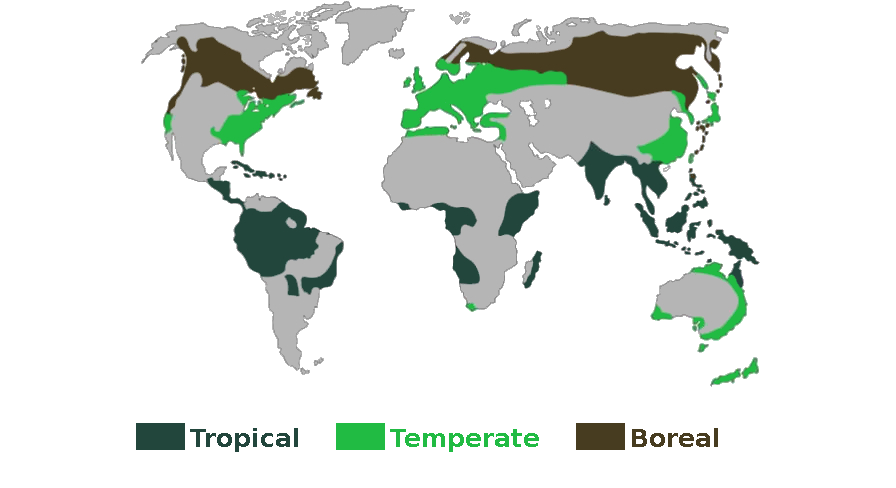
\includegraphics[width=\textwidth]{Figures/forest_in_world}
\caption{Forest repartition in the world.}
\label{fig:forest_in_world}
\end{center}
\end{figure}

Forests at different latitudes and elevations form distinctly different ecozones: boreal forests near the poles, tropical forests near the equator and temperate forests at mid-latitudes (see Figure~\ref{fig:forest_in_world}). Higher elevation areas tend to support forests similar to those at higher latitudes, and amount of precipitation also affects forest composition. Since these ecozones are very different, the study of forested areas must be restricted to a single ecozone at a time.

Forests are the dominant terrestrial ecosystem of Earth, and are distributed across the globe \citep{pan2013structure}. Forests account for 75\% of the gross primary productivity of the Earth's biosphere, and contain 80\% of the Earth's plant biomass \citep{pan2013structure}. They also hold about 90\% of terrestrial biodiversity.

Forests are also benefit for the environment; they capt and store the CO$_{2}$ \citep{fahey2010forest} (see Figure~\ref{fig:carbon_cycle}). About 45\% of the total global carbon is held by forests. They also filter dust and microbial pollution of the air \citep{smith2012air}. Finally, They also play an important role in hydrological regulation and water purification \citep{lempriere2008importance} (see Figure~\ref{fig:carbon_cycle}).

\begin{figure}[htbp]
\begin{center}
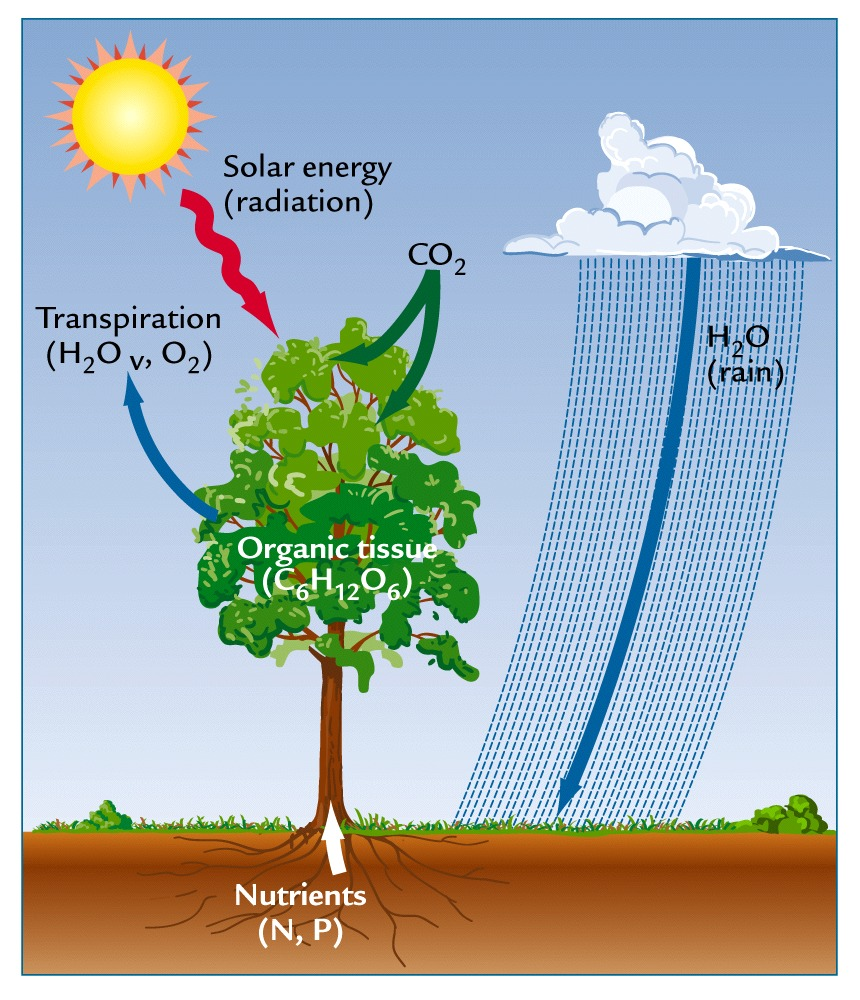
\includegraphics[width=0.5\textwidth]{Figures/carbon_cycle}
\caption{Carbon cycle: a process of CO$_{2}$ storage, water and air purification.}
\label{fig:carbon_cycle}
\end{center}
\end{figure}

Human society and forests influence each other in both positive and negative ways \citep{vogt2006global}. Forests provide ecosystem services to humans and serve as tourist attractions. Forests can also affect people's health. Human activities, including harvesting forest resources, can negatively affect forest ecosystems. Wood from forest has many uses. It has been widely used for fuel \citep{sterrett1994alternative}. In this case, hardwood is preferred over softwood because it creates less smoke and burns longer.  Wood is still an important construction material \citep{ramage2017wood}: Elm was used for the construction of wood boats. In Europe, oak is still the the wood of choice for all wood constructions, including beams, walls, doors, and floors. A wider variety of woods is also used such as poplar, small-knotted pine, and Douglas fir. Wood is also needed in the paper industry since wood fibers are an important component of most paper. Eventually, wood is also extensively used for furniture or for making tools or music instruments.

In order to exploit the forest resources, a precise mapping of forests is needed.
Forests are complex structures \citep{pommerening2002approaches}, for which informations are needed for management and exploitation. The information can be the tree species or the tree maturity of the forest. There are two ways to extract such information from forest; field inventory or remote sensing. The field inventories are very expensive to set up and are also not adapted for a national study. A more adapted to obtain such information is remote sensing since it allows to extract them at a large scale. \\

\section{Remote sensing for forested areas}

The analysis of forested areas from a remote sensing point of view can be performed at three different levels: pixel, object (mainly trees) or stand. In statistical national forest inventory (NFI), an automated and accurate tree segmentation is needed in order to extract tree level features (basal area, dominant tree height, etc., \citep{means2000predicting,Malatamo}). However, the tree level is not the only reliable level of analysis for forest studies. When a joint mapping and statistical reasoning is required (e.g., land-cover (LC) mapping and forest inventory), forest stands remain the prevailing scale of analysis \citep{means2000predicting,White2016CJRS}. A stand can be defined in many different ways in terms of homogeneity: tree specie, age, height, maturity, and its definition varies according to the countries. \\

From a remote sensing point of view, the delineation of the stands is a segmentation problem. Forest stands are interesting in order to extract reliable and statistically meaningful features and to provide an input for multi-source statistical inventory. For land-cover mapping, this is highly helpful for forest database updating \citep{Kim09}, whether the labels of interest are \textit{vegetated areas} {(e.g., \textit{deciduous/evergreen/mixed/non-forested)}}, or, even more precisely, the tree species. Most of the time in national forestry inventory institutes, for reliability purposes, each area is manually interpreted by human operators with very high resolution (VHR) geospatial images focusing on the infra-red channel \citep{Malatamo}. This work is extremely time consuming and subjective \citep{Wulder2008}. Furthermore, in many countries, the wide variety of tree species (e.g., $>$20) significantly complicates the problem. The design of an automatic procedure based on remote sensing data would fasten such process. Additionally, the standard manual delineation procedure only takes into account the species, and few characteristics (alternatively height, age, stem density or crown closure), while an automatic method could offer more flexibility and would allow to combine characteristics extracted from all complementary data sources. \\

The use of remote sensing data for the automatic analysis of forests has been growing in the last 15 years, especially with the synergistic use of airborne laser scanning (ALS) and optical VHR imagery (multispectral imagery and hyperspectral imagery) \citep{torabzadeh2014fusion,White2016CJRS}. They appear to be both well adapted and complementary inputs for stand segmentation \citep{dalponte2012tree,dalponte2015delineation,7500049}. ALS provides a direct access to the vertical distribution of the trees and to the ground underneath. Hyperspectral and multispectral images are particularly relevant for tree species classification: spectral and textural information from VHR  images can allow a fine discrimination of many species, respectively. Multispectral images are often preferred due to their higher availability, and higher spatial resolution. Multispectral images can be acquired from airplanes or satellites. Spaceborne sensors allows to capture large areas with a high repeatability but suffer from a low spatial resolution (see Table~\ref{table:spatial_satellites}). For a better spatial resolution, airborne multispectral images are preferred. The airborne linear lidar has been widely used for remote sensing tasks \citep{lim2003lidar, shan2008topographic, vosselman2010airborne}. The new geiger mode lidar is also very promising, allowing a hight point density with different angles at a higher altitude \citep{ullrich2016linear}. \\

\begin{sidewaystable}
\begin{center}
%\todo[inline]{http://fr.wikipedia.org/wiki/SPOT http://www.satimagingcorp.com/gallery.html}

\begin{small}
\begin{tabular}{l|c|c|c|c|c|c|c}

%Images
%& 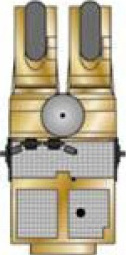
\includegraphics[height=2cm]{Figures/satellites/spot_123} & 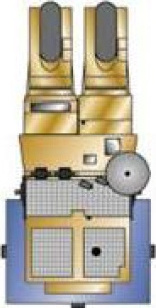
\includegraphics[height=2cm]{Figures/satellites/spot_4} & 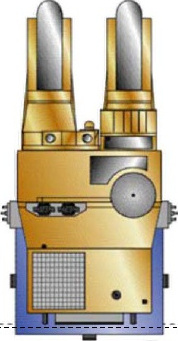
\includegraphics[height=2cm]{Figures/satellites/spot_5} & 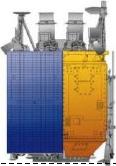
\includegraphics[height=2cm]{Figures/satellites/spot_67} & & & 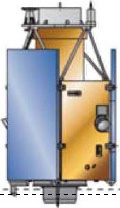
\includegraphics[height=2cm]{Figures/satellites/pleiades} \\

%Nom
& \textbf{SPOT 1,2,3} & \textbf{SPOT 4} & \textbf{SPOT 5} & \textbf{SPOT 6,7} & \textbf{Ikonos} & \textbf{Quickbird} &\textbf{Pléiades} \\
\hline
%
Swath & & 60 km & 60 km & 60 km & 11 km & 16.5 km & 20 km \\
%
Revisit time & 3 d & 2 d & 2 d & 2 d & 3 d & 1-3.5 d & 1 d \\
%
Resolution PAN & 10 m & 10 m & 2,5 m or 5 m & 1,5 m & 1 m & 0.61-0.72 m & 0,7 m \\
%
Resolution XS & 20 m & 20 m & 10 m & 6 m & 4 m & 2.44-2.88 m & 2,8 m \\
%
Spectral Bands (nm) & & & & & & \\
%
- PAN & 500-730 & 610-680 & 480-710 & 450-750 & 450-900 & 450-900 & 470-830 \\
%
- Blue & - & - & - & 455-520 & 450-530 & 450-520 & 430-550 \\
%
- Green & 500-590 & 500-590 & 500-590 & 530-600 & 520-610 & 520-600 & 500-620 \\
%
- Red & 610-680 & 610-680 & 610-680 & 620-690 & 640-720 & 630-690 & 590-710 \\
%
- NIR & 780-890 & 780-890 & 780-890 & 760-890 & 760-880 & 760-900 & 740-940 \\
\end{tabular}
\end{small}
\end{center}
\caption{Principal multispectral spatial optical sensors.}
\label{table:spatial_satellites}
\end{sidewaystable}

A prerequisite for data fusion is the most accurate alignment of the two data \citep{torabzadeh2014fusion}. A frequently used technique is to geo-rectify images using ground controls points (GCPS). A geometric transformation is established between the coordinates of GCPs and their corresponding pixels in the image. It is then applied for each pixel, so that coordinate differences on those checkpoints are reduced to the lowest possible level. This method can be easily applied and is relatively fast in terms of computation time. However the use of GCPs can still cause that the unknowns in the trajectory of the platforms produce some remarkable residual errors. Automatic methods for data registration have also been developed \citep{habib2005photogrammetric,mastin2009automatic}. \\

\section{Context of the thesis}
In France, the study of forests is two fold. They need to be mapped and inventoried. The forest inventory allows to obtain an estimation of the wood stock and the forestation rate at a national scale (see Figures~\ref{fig:wood_volume}~\&~\ref{fig:forestation}). Statistics such as volume per hectare, deciduous volume or conifer volume can then be derived. The inventory is performed through field inventory and extrapolated using the forest mapping. Thus, the mapping of forest is very important in order to derive accurate statistics.	
The forest mapping is given by a national forest LC database (see Figure~\ref{fig:FLC}). It is manually interpreted by human operators using VHR infra-red colored (IRC) ortho-images. It assigns a vegetation type to each mapped beach of more than 5000$\:$m$^{2}$. The nomenclature is composed of 32 classes based on hierarchical criteria such as pure stands of the main tree species of the French forest. The forest LC should be updated in a 10 years cycle.

\begin{figure}[htbp]
\begin{center}
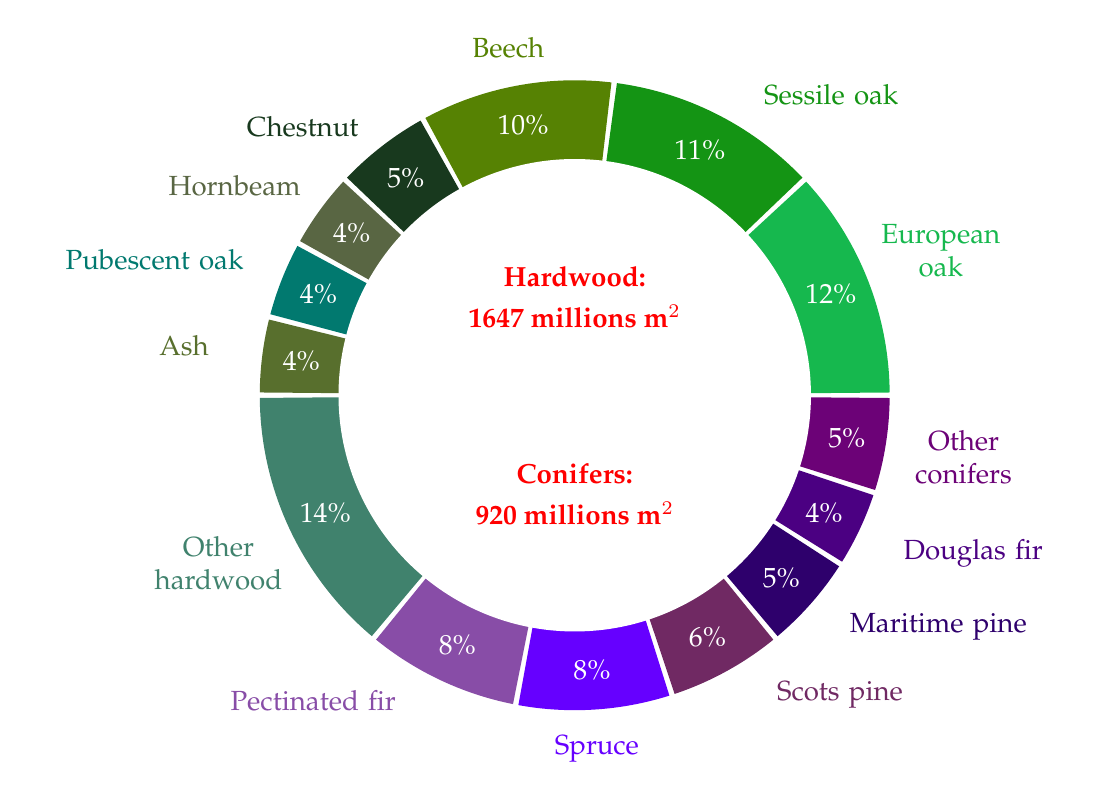
\begin{tikzpicture}
\def\rb{3}
\def\re{4}
\newcommand{\col}{red}

\newcommand{\arccam}[3]
{
\def\rb{3}
\def\re{4}
\def\ab{#1}
\def\ae{#2}
\def\co{#3}
\draw[fill=\co,draw=none] (0,0) -- (\ab:\re) arc (\ab:\ae:\re) -- (0,0);
}

\definecolor{perso}{RGB}{22, 184, 78}
\renewcommand{\col}{perso}


\pgfmathsetmacro\abb{0}
\pgfmathsetmacro\aee{0.12*360}
\arccam{\abb+0.5}{\aee-0.5}{\col}
\pgfmathsetmacro\amid{(\abb+\aee)/2}
\pgfmathsetmacro\px{3.5*cos(\amid)}
\pgfmathsetmacro\py{3.5*sin(\amid)}
\node[color=white] at (\px,\py) {12\%};
\pgfmathsetmacro\px{5*cos(\amid)}
\pgfmathsetmacro\py{5*sin(\amid)}
\node[color=\col,text width=50, text centered] at (\px,\py) {European oak};


\definecolor{perso}{RGB}{20, 148, 20}
\pgfmathsetmacro\abb{\aee}
\pgfmathsetmacro\aee{\abb+0.11*360}
\arccam{\abb+0.5}{\aee-0.5}{\col}
\pgfmathsetmacro\amid{(\abb+\aee)/2}
\pgfmathsetmacro\px{3.5*cos(\amid)}
\pgfmathsetmacro\py{3.5*sin(\amid)}
\node[color=white] at (\px,\py) {11\%};
\pgfmathsetmacro\px{4.0*cos(\amid)}
\pgfmathsetmacro\py{4.0*sin(\amid)}
\node[color=\col,text width=75, text centered, anchor=south west] at (\px,\py) {Sessile oak};


\definecolor{perso}{RGB}{86, 130, 3}
\pgfmathsetmacro\abb{\aee}
\pgfmathsetmacro\aee{\abb+0.10*360}
\arccam{\abb+0.5}{\aee-0.5}{\col}
\pgfmathsetmacro\amid{(\abb+\aee)/2}
\pgfmathsetmacro\px{3.5*cos(\amid)}
\pgfmathsetmacro\py{3.5*sin(\amid)}
\node[color=white] at (\px,\py) {10\%};
\pgfmathsetmacro\px{4.5*cos(\amid)}
\pgfmathsetmacro\py{4.5*sin(\amid)}
\node[color=\col,text width=50, text centered] at (\px,\py) {Beech};


\definecolor{perso}{RGB}{24, 57, 30}
\pgfmathsetmacro\abb{\aee}
\pgfmathsetmacro\aee{\abb+0.05*360}
\arccam{\abb+0.5}{\aee-0.5}{\col}
\pgfmathsetmacro\amid{(\abb+\aee)/2}
\pgfmathsetmacro\px{3.5*cos(\amid)}
\pgfmathsetmacro\py{3.5*sin(\amid)}
\node[color=white] at (\px,\py) {5\%};
\pgfmathsetmacro\px{4.0*cos(\amid)}
\pgfmathsetmacro\py{4.0*sin(\amid)}
\node[color=\col,text width=50, text centered, anchor=south east] at (\px,\py) {Chestnut};


\definecolor{perso}{RGB}{89, 102, 67}
\pgfmathsetmacro\abb{\aee}
\pgfmathsetmacro\aee{\abb+0.04*360}
\arccam{\abb+0.5}{\aee-0.5}{\col}
\pgfmathsetmacro\amid{(\abb+\aee)/2}
\pgfmathsetmacro\px{3.5*cos(\amid)}
\pgfmathsetmacro\py{3.5*sin(\amid)}
\node[color=white] at (\px,\py) {4\%};
\pgfmathsetmacro\px{4.1*cos(\amid)}
\pgfmathsetmacro\py{4.1*sin(\amid)}
\node[color=\col,text width=50, text centered,anchor=south east] at (\px,\py) {Hornbeam};


\definecolor{perso}{RGB}{1, 121, 111}
\pgfmathsetmacro\abb{\aee}
\pgfmathsetmacro\aee{\abb+0.04*360}
\arccam{\abb+0.5}{\aee-0.5}{\col}
\pgfmathsetmacro\amid{(\abb+\aee)/2}
\pgfmathsetmacro\px{3.5*cos(\amid)}
\pgfmathsetmacro\py{3.5*sin(\amid)}
\node[color=white] at (\px,\py) {4\%};
\pgfmathsetmacro\px{4.0*cos(\amid)}
\pgfmathsetmacro\py{4.0*sin(\amid)}
\node[color=\col,text width=85, text centered,anchor=south east] at (\px,\py) {Pubescent oak};


\definecolor{perso}{RGB}{88, 111, 45}
\pgfmathsetmacro\abb{\aee}
\pgfmathsetmacro\aee{\abb+0.04*360}
\arccam{\abb+0.5}{\aee-0.5}{\col}
\pgfmathsetmacro\amid{(\abb+\aee)/2}
\pgfmathsetmacro\px{3.5*cos(\amid)}
\pgfmathsetmacro\py{3.5*sin(\amid)}
\node[color=white] at (\px,\py) {4\%};
\pgfmathsetmacro\px{5*cos(\amid)}
\pgfmathsetmacro\py{5*sin(\amid)}
\node[color=\col,text width=50, text centered] at (\px,\py) {Ash};


\definecolor{perso}{RGB}{64, 130, 109}
\pgfmathsetmacro\abb{\aee}
\pgfmathsetmacro\aee{\abb+0.14*360}
\arccam{\abb+0.5}{\aee-0.5}{\col}
\pgfmathsetmacro\amid{(\abb+\aee)/2}
\pgfmathsetmacro\px{3.5*cos(\amid)}
\pgfmathsetmacro\py{3.5*sin(\amid)}
\node[color=white] at (\px,\py) {14\%};
\pgfmathsetmacro\px{5*cos(\amid)}
\pgfmathsetmacro\py{5*sin(\amid)}
\node[color=\col,text width=70, text centered] at (\px,\py) {Other hardwood};

%%%%%%%%%%%%%%%%%%%%%%%%%%%%%%%%%%%%%%%%%%%%%%%%%%

\definecolor{perso}{RGB}{136, 77, 167}
\pgfmathsetmacro\abb{\aee}
\pgfmathsetmacro\aee{\abb+0.08*360}
\arccam{\abb+0.5}{\aee-0.5}{\col}
\pgfmathsetmacro\amid{(\abb+\aee)/2}
\pgfmathsetmacro\px{3.5*cos(\amid)}
\pgfmathsetmacro\py{3.5*sin(\amid)}
\node[color=white] at (\px,\py) {8\%};
\pgfmathsetmacro\px{4.0*cos(\amid)}
\pgfmathsetmacro\py{4.0*sin(\amid)}
\node[color=\col,text width=85, text centered, anchor=north east] at (\px,\py) {Pectinated fir};


\definecolor{perso}{RGB}{102, 0, 255}
\pgfmathsetmacro\abb{\aee}
\pgfmathsetmacro\aee{\abb+0.08*360}
\arccam{\abb+0.5}{\aee-0.5}{\col}
\pgfmathsetmacro\amid{(\abb+\aee)/2}
\pgfmathsetmacro\px{3.5*cos(\amid)}
\pgfmathsetmacro\py{3.5*sin(\amid)}
\node[color=white] at (\px,\py) {8\%};
\pgfmathsetmacro\px{4.5*cos(\amid)}
\pgfmathsetmacro\py{4.5*sin(\amid)}
\node[color=\col,text width=50, text centered] at (\px,\py) {Spruce};


\definecolor{perso}{RGB}{112, 41, 99}
\pgfmathsetmacro\abb{\aee}
\pgfmathsetmacro\aee{\abb+0.06*360}
\arccam{\abb+0.5}{\aee-0.5}{\col}
\pgfmathsetmacro\amid{(\abb+\aee)/2}
\pgfmathsetmacro\px{3.5*cos(\amid)}
\pgfmathsetmacro\py{3.5*sin(\amid)}
\node[color=white] at (\px,\py) {6\%};
\pgfmathsetmacro\px{4.0*cos(\amid)}
\pgfmathsetmacro\py{4.0*sin(\amid)}
\node[color=\col,text width=75, text centered, anchor=north west] at (\px,\py) {Scots pine};


\definecolor{perso}{RGB}{46, 0, 108}
\pgfmathsetmacro\abb{\aee}
\pgfmathsetmacro\aee{\abb+0.05*360}
\arccam{\abb+0.5}{\aee-0.5}{\col}
\pgfmathsetmacro\amid{(\abb+\aee)/2}
\pgfmathsetmacro\px{3.5*cos(\amid)}
\pgfmathsetmacro\py{3.5*sin(\amid)}
\node[color=white] at (\px,\py) {5\%};
\pgfmathsetmacro\px{4.0*cos(\amid)}
\pgfmathsetmacro\py{4.0*sin(\amid)}
\node[color=\col,text width=85, text centered, anchor=north west] at (\px,\py) {Maritime pine};


\definecolor{perso}{RGB}{75, 0, 130}
\pgfmathsetmacro\abb{\aee}
\pgfmathsetmacro\aee{\abb+0.04*360}
\arccam{\abb+0.5}{\aee-0.5}{\col}
\pgfmathsetmacro\amid{(\abb+\aee)/2}
\pgfmathsetmacro\px{3.5*cos(\amid)}
\pgfmathsetmacro\py{3.5*sin(\amid)}
\node[color=white] at (\px,\py) {4\%};
\pgfmathsetmacro\px{4.0*cos(\amid)}
\pgfmathsetmacro\py{4.0*sin(\amid)}
\node[color=\col,text width=75, text centered, anchor=north west] at (\px,\py) {Douglas fir};


\definecolor{perso}{RGB}{108, 2, 119}
\pgfmathsetmacro\abb{\aee}
\pgfmathsetmacro\aee{\abb+0.05*360}
\arccam{\abb+0.5}{\aee-0.5}{\col}
\pgfmathsetmacro\amid{(\abb+\aee)/2}
\pgfmathsetmacro\px{3.5*cos(\amid)}
\pgfmathsetmacro\py{3.5*sin(\amid)}
\node[color=white] at (\px,\py) {5\%};
\pgfmathsetmacro\px{5*cos(\amid)}
\pgfmathsetmacro\py{5*sin(\amid)}
\node[color=\col,text width=50, text centered] at (\px,\py) {Other conifers};


\draw[fill=white,draw=none] (0,0) circle (\rb);

\definecolor{perso}{RGB}{255,0,0}
\node[color=\col] at (0,-1) {\textbf{Conifers: }};
\node[color=\col] at (0,-1.5) {\textbf{920 millions m$^{2}$}};
\node[color=\col] at (0,1.5) {\textbf{Hardwood: }};
\node[color=\col] at (0,1) {\textbf{1647 millions m$^{2}$}};

\end{tikzpicture}
\caption{Distribution wood volume per species.}
\label{fig:wood_volume}
\end{center}
\end{figure}

\begin{figure}
\begin{center}
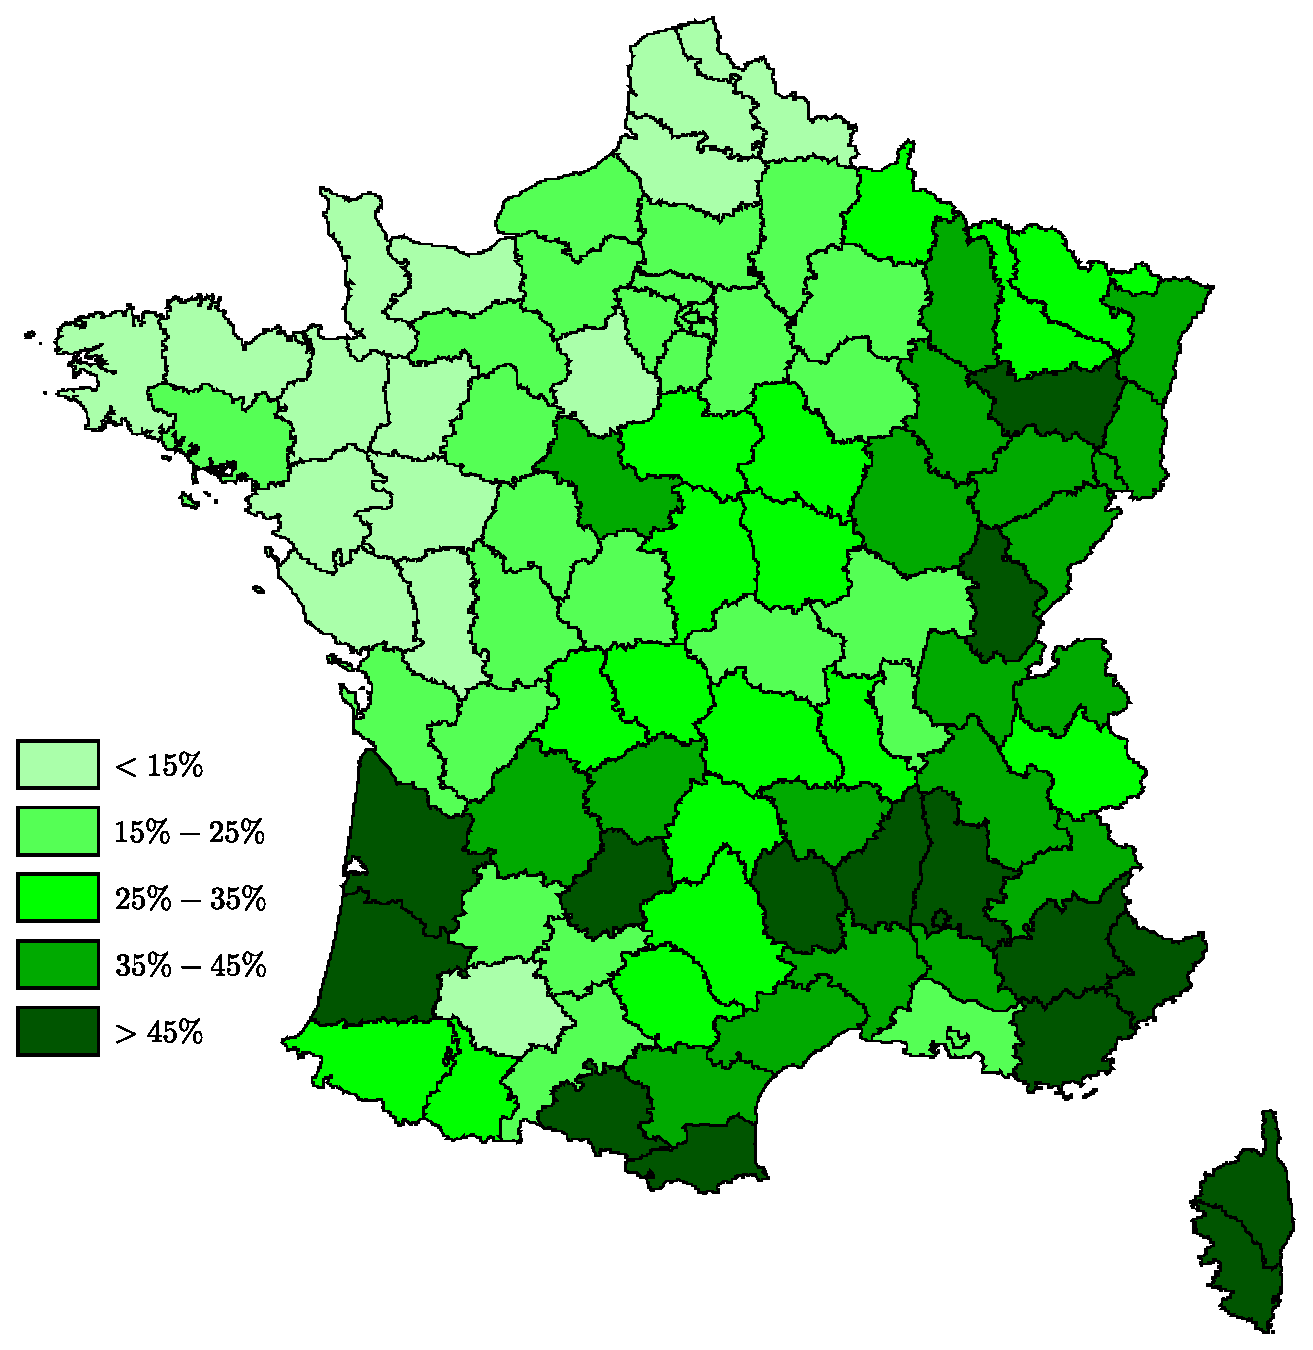
\includegraphics[width=0.8\textwidth]{Figures/boisement}
\end{center}
\caption{Forestation rate in France.}
\label{fig:forestation}
\end{figure}

\begin{figure}[htbp]
\begin{center}
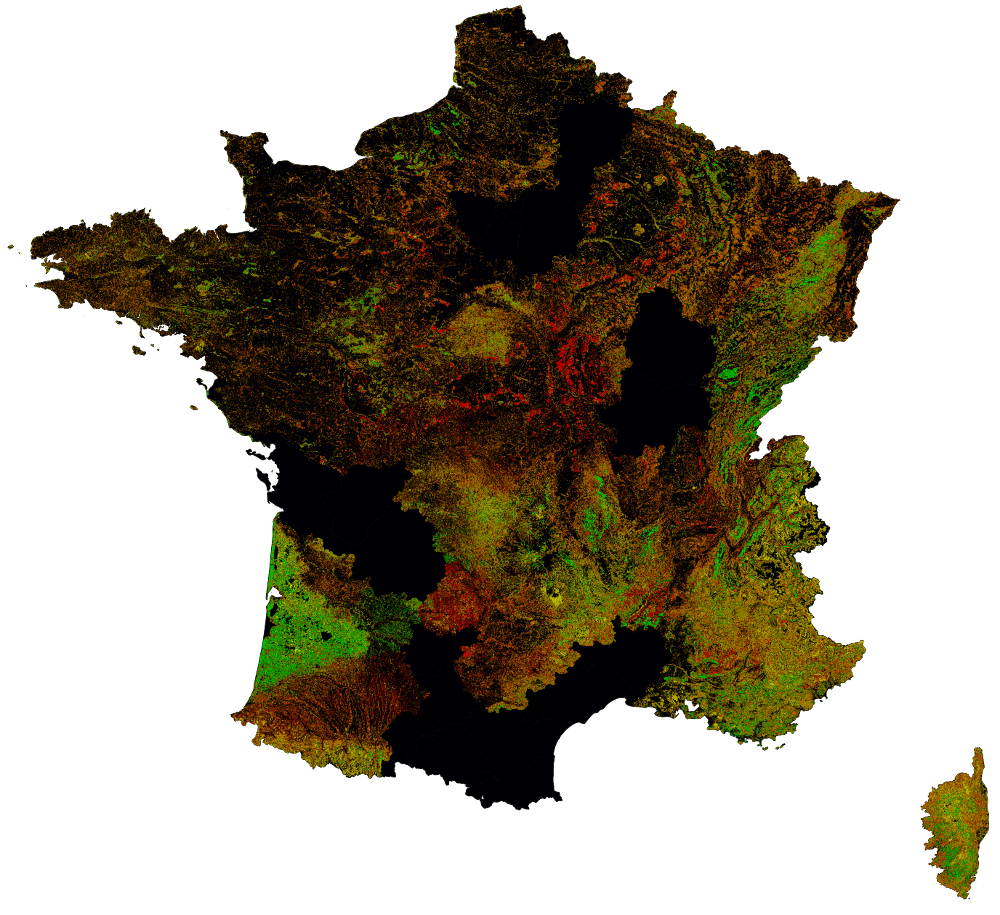
\includegraphics[width=\textwidth]{Figures/BD_foret_France_2}
\end{center}
\caption{The French forest LC. Each color is associated to a single specie ($\sim$20 species in total), black corresponds to non-labeled zones (not operated or non forested).}
\label{fig:FLC}
\end{figure}


\section{Objectives}
Currently, the forest LC is obtained through remote sensing (namely photo-inter\-pretation), an method could be developed to update it automatically. Since an old version of the forest LC is available, it can be used as a ground truth input for subsequent classification \citep{gressin2013updating}. However, the learning process should be carried out carefully \citep{gressin2014updating}. Indeed, some area might have change (e.g. forest cuts). Furthermore, the database is designed generalized \citep{smith1977database}. A simple classification would then not be sufficient in order to retrieve homogeneous patches similar to the forest LC. Indeed, forests are not perfectly homogeneous in term of species and there can be many holes in the canopy, leading to a noisy classification. In order to retrieve homogeneous patches, the classification could be regularized using smoothing methods \citep{schindler2012overview}. Furthermore, an automatic method would allow to enrich the LC, i.e. retrieve homogeneous tree species stands also homogeneous in terms of height \citep{gressin2014unified}.

\section{Strategy}
Two remote sensing modalities are available for the mapping of forested areas at IGN; VHR optical images and lidar cloud points. The VHR images are a part of a national database. In this thesis, the images used have a spatial resolution of 50$\:$cm. Two type of ortho-images are available, a color image (3 bands; red: 600-720$\:$nm, green: 490-610$\:$nm and blue: 430-550$\:$nm) and and IRC image (3 bands; near infra-red: 750-950$\:$nm, red and green) captured by the IGN digital cameras \citep{souchon2012large}. It is then possible to obtain four band ortho-images by the combination of the two ortho-images type. \\
IGN also process lots of test flight over forested areas with a laser scanning device. The airborne lidar data were collected using an Optech 3100EA device. The footprint was 0.8$\:$m in order to increase the probability to reach the ground. The point density {for all echoes} ranges from 2 to 4$\:$points/m$^{2}$. \\

The registration between airborne lidar point clouds and VHR multispectral images was performed by IGN itself using ground control points. This is a standard procedure in the French mapping agency since IGN operates both sensors and has also a strong expertise in data georeferencing (this is in fact the national institute responsible for that in France for both airborne and spaceborne sensors). \\
Data were acquired under leaf-on conditions and fit with the standards used in many countries for large-scale operational forest mapping purposes. \\

The combination of these two data is very relevant for the study of forest, indeed, optical images provide the major information about the tree species, while lidar give information about the vertical structure of the forest. Furthermore, the lidar allows to extract consistent object such as trees. \\

In order to extract more information from these two modalities, the fusion should be performed at different levels. 3 levels could be defined:
\begin{itemize}
%\addtolength{\itemindent}{3cm}
\item[$\bullet$] Low level: It corresponds to the fusion of the observations, in this case, only the reflectance from the optical images and the height of the lidar points.
\item[$\bullet$] Medium level: It corresponds to the fusion of the features, they are derived at the same level (e.g. the pixel) and merged together. It also corresponds to the cooperative understanding of the data; a feature is derived on a modality (e.g. trees from lidar) and use on the other.
\item[$\bullet$] High level: It corresponds to the fusion of decision. One or many classifications have been performed and the final decision is a smart combination of the classifications and the input data.
\end{itemize}

\section{Structure of the thesis}

\begin{itemize}
\item State of the art: Chapter \ref{Chapter1}
\item Method: Chapter \ref{Chapter2}
\item Results: Chapter \ref{Chapter3}
\item Conclusion and perspectives: Chapter \ref{Conclusion}
\end{itemize}

\stopcontents[chapters]

\openchapter
% Chapter 1
\chapter{State of the art} % Main chapter title
\label{Chapter1} % For referencing the chapter elsewhere, use \ref{Chapter1} 

\startcontents[chapters]
\Mprintcontents


%----------------------------------------------------------------------------------------

% Define some commands to keep the formatting separated from the content

%----------------------------------------------------------------------------------------

Forest are complex areas, the mapping of such environment needs the use of different image processing methods. The extraction of "homogeneous" forest stands is at the interplay between different kinds of image processing methods. Segmentation algorithms can be employed for a fine or coarse delineation of the principal components of the forests. Classification is also very useful to discriminate the different elements of the forest. Eventually, smoothing methods, such as graph cut, are used for a refinement of raw results.

\section{Stand segmentation}
A forest stand is defined as a contiguous group of trees that are uniform in specie composition, structure, age and/or height, spatial arrangement, site quality or condition to distinguish it from adjacent other groups of trees.

One should note that the literature remains mostly focused on individual tree extraction and tree species classification \citep{dalponte2014tree, vega2014ptrees, kandare2014new, }, developing site-specific workflows with similar advantages, drawbacks and classification performance. More authors have focused on forest delineation \citep{eysn2012forest}, that do not convey information about the tree species and their spatial distribution. Even if some methods have proposed forest stand delineation, they remain very specific to the study area. Consequently, no operational framework embedding the automatic analysis of remote sensing data has been yet proposed in the literature for forest stand segmentation at large scale \citep{clement_IJPRS}. \\

Hence, in the large amount of literature in the field, only few papers focus on the issue of stand segmentation or delineation. They can be categorized with regard to the type of data processed. \\
\subsection{Stand segmentation using VHR optical images}
A stand delineation technique using VHR airborne hyperspectral imagery is proposed in \citep{leckie2003stand}. The trees are extracted using a valley following approach and classified into 7 tree species (5 coniferous, 1 deciduous, and 1 non-specified) with a maximum likelihood classifier. A semi-automatic iterative clustering procedure is then introduced to generate the forest polygons.\\
A hierarchical and multi-scale approach for the identification of stands is adopted in \citep{hernando2012spatial}. The data inputs were the 4 bands of an airborne 0.5$\:$m orthoimage (Red, Green, Blue, and Near Infra-Red) allowing to derive the Normalized Difference Vegetation Index (NDVI). The stand mapping solution is based on the Object-Based Image Analysis concept. It is composed of two main phases in a cyclic process: first, segmentation, then classification. The first level consists in over-segmenting the area of interest and performing fine-grained land cover classification. The second level aims to transfer the vegetation type provided by a land cover geodatabase in the stand polygons, already retrieved from another segmentation procedure. The multi-scale analysis appears to have a significant benefit on the stand labeling but it is highly heuristic and requires a correct definition of the stand while we consider it is an interleaved problem. \\
Following the work of \citep{Wulder2008} with IKONOS images, Quickbird-2 panchromatic images are used in \citep{Mora20102474} to automatically delineate forest stands. A standard image segmentation technique is used and the novelty mainly lies on the fact that its initial parameters are optimized with respect to NFI protocols. They show that meaningful stand heights can be derived, which are a critical input for various modeled inventory attributes.\\

\subsection{Stand segmentation using lidar}
A seminal stand mapping method using low density airborne lidar data is proposed in \citep{koch2009airborne}. It is composed of several steps of feature extraction, creation and raster-based classification. Forest stands are created by grouping neighboring cells within each class. Then, only the stands with a pre-defined minimum size are accepted. Neighboring small areas of different forest types that do not reach the minimum size are merged together to an existing forest stand. The approach offers the advantage of detecting 15 forest types that match very well with the ground truth but to the detriment of simplicity: the flowchart has to be highly reconsidered to fit to other stand specifications. Additionally, the tree species discrimination is not addressed.\\
The forest stand delineation proposed in \citep{sullivan2009object} also uses low density airborne lidar still coupling an object-oriented image segmentation and a supervised classification procedure. Three features are computed and rasterized. The segmentation is performed using a region growing approach. Spatially adjacent pixels are grouped into homogeneous discrete image objects or regions. Then, a supervised discrimination of the segmented image is performed using a Battacharya classifier, in order to determine the maturity of the stands. The tree species are ignored and the procedure requires a careful inspection of the raw data both for feature generation and model training. \\
The method proposed in \citep{eysn2012forest} aims to generate a forest mask (\textit{forested area} label only) using low density airborne lidar. A Canopy Height Model (CHM) with a spatial resolution of 1$\:$m is derived. The positions and heights of single trees are determined from the CHM using a local maximum filter, based on a moving window approach. Only detected positions with a CHM height superior to 3$\:$m are considered. The crown radii are estimated using an empirical function. The three neighboring trees are connected using a Delaunay triangulation applied to the previously-detected tree position. The crown cover is then calculated using the crown areas of three neighboring trees and the area of their convex hull for each tree triple. The forest mask is derived from the canopy cover values. While this is not a genuine stand delineation method, this approach could be easily extended to a multi-class problem and enlightens the necessity of individual tree extraction even with limited point densities as a basis for the stand-level analysis.\\
A forest stand delineation also based on airborne lidar data is proposed in \citep{wu2014data}. Three features are first directly extracted from the point cloud. A coarse forest stand delineation is then performed on the feature image using the unsupervised Mean-Shift algorithm, in order to obtain under-segmented raw forest stands. A forest mask is then applied to the segmented image in order to retrieve forest and non-forest raw stands. It may create some small isolated areas, iteratively merged to their most similar neighbor until their size is larger than a user-defined threshold in order to product big raw forest stands. They are then refined into finer level using a seeded region growing based on superpixels. The idea is to select several different superpixels in a raw forest stand and merge them. This method provides a coarse-to-fine segmentation with relatively large stands. The process was only applied on a small area of a forest in Finland, thus, general conclusions can not be drawn. \\

\subsection{Stand segmentation using VHR optical images and lidar}
The analysis of the lidar and multispectral data is performed at three levels in \citep{tiede2004object}, following a given hierarchical nomenclature of classes in forested environments. The first level represents small objects (single tree scale, individual trees or small groups of trees) that can be differentiated by spectral and structural characteristics using a rule-based classification. The second level corresponds to the stand level. It is built using the same classification process which summarizes forest development phases by referencing to small scale sub-objects at level 1. The third level is generated by merging objects of the same classified forest-development into larger spatial units. The multi-scale analysis offers the advantage of alleviating the standard issue of individual tree crown detection and proposing development stage labels. Nevertheless, the pipeline is highly heuristic, under-exploits lidar data and significant confusions between classes are reported.\\
The automatic segmentation process of forests in \citep{diedershagen2004automatic} is also supplied with Lidar and VHR multispectral images. The idea is to divide the forests into higher and lower sections with lidar. An unsupervised classification process is applied to the two images. The final stand delineation is achieved by segmenting the classification results with pre-defined thresholds. The segmentation results are improved using morphological operators such as opening and closing, which fill the gaps and holes at a specified extent. This method is efficient if the canopy structure is homogeneous and requires a strong knowledge on the area of interest. Since it is based on height information only, it cannot differentiate two stands of similar height but different species.\\
In \citep{leppanen2008automatic} a stand segmentation technique for a forest composed of \textit{Scots Pine}, \textit{Norway Spruce} and \textit{Hardwood} is defined. A hierarchical segmentation on the Crown Height Model followed by a restricted iterative region growing approach is performed on images composed of rasterized lidar data and Colored Infra-Red images. The process was only applied on a limited area of Finland and prevents from drawing strong conclusions. However, the quantitative analysis carried out by the authors shows that lidar data can help to define statistically meaningful stands (here the criterion was the timber volume) and that multispectral images are inevitable inputs for tree species discrimination. \\

\subsection{Challenges of stand segmentation}
The Table~\ref{table:methods} summarize the presented methods of forest stands segmentation. 
\begin{sidewaystable}[htbp]
\begin{center}
\begin{tabular}{|l|c|c|c|}
\hline
Reference & Data processed & Country & Segmentation criteria \\
\hline
\cite{leckie2003stand} & Hyperspectral images & Canada & 7 tree species \\
\hline
\cite{hernando2012spatial} & Multispectral images & Spain & Vegetation type \\
\hline
\cite{Mora20102474} & Panchromatic images & Canada & Height \\
\hline
\cite{koch2009airborne} & Lidar & Germany & 15 forest types \\
\hline
\cite{sullivan2009object} & Lidar & USA & Tree maturity \\
\hline
\cite{eysn2012forest} & Lidar &  Austria & Forest mask \\
\hline
\cite{wu2014data} & Lidar & Finland & Tree size, tree density \\
\hline
\cite{tiede2004object} & Lidar and multispectral images & Germany & Development phase \\
\hline
\cite{diedershagen2004automatic} & Lidar and multispectral images & Germany & Canopy structure, height \\
\hline
\cite{leppanen2008automatic} & Lidar and multispectral images & Finland & 3 tree species \\
\hline
\end{tabular}
\caption{Existing methods for forest stand segmentation.}
\label{table:methods}
\end{center}
\end{sidewaystable}

Regarding the existing state of the art on the forest stand segmentation, it appears that such task is very complex to implement. Indeed, a simple segmentation is not sufficient since it does not allows to retrieve consistent stands. A classification is mandatory in order to obtain the tree species. However, it is very difficult to discriminate species, since some have a very close looking (e.g. deciduous oak and beech). Eventually, the stands are not totally pure, a certain level of generalization is desired in order to have a consistent mapping at large scale. Thus, a regularization process can be employed for such purpose.
It also appears that the type of data employed has an impact on the results.
\begin{itemize}
\item The VHR optical images permits to obtain information about the tree species, especially when using texture features.
\item The lidar data provide information about the vertical structure of the forest that can also be useful for the discrimination of tree species \citep{brandtberg2007classifying}. It also brings information about the height that allows to separate forest stands of different ages. Most of the time, lidar is deeply under exploited since it is used only as a simple DSM.
\end{itemize}

\section{Segmentation}
\label{sec:C1_seg}
The direct segmentation of the optical image and/or the lidar point clouds is not sufficient in order to retrieve forest stands. Indeed, such segmentation methods can not take into account the information needed to define the stand.  However, with adapted parameters, segmentations algorithms might be useful to obtain relevant segmentation of the data \citep{clement_IJPRS}. They can be divide in two categories:
\begin{itemize}
\item The pure segmentation methods, in these methods, a specific attention must be paid to the choice of the parameters in order to obtain a relevant over-segmentation. Such segmentation can be applied on an image or a point cloud. Specific methods have also been developed for the segmentation of lidar point cloud \citep{nguyen20133d}.
\item The superpixels segmentation methods, they natively produce an over-segmentation of the image. The parameters control the size and the shape of the resulting segments.
\end{itemize}

\subsection{Traditional segmentation methods}
The segmentation of an image can be performed using number of techniques \citep{pal1993review}. \\

The easiest way to segment an image is the thresholding of a gray level histogram of the image \citep{taxt1989segmentation}. When the image is noisy or the background is uneven and illumination is poor, such thresholding is not sufficient. Thus, adaptive thresholding methods have been developed \citep{yanowitz1989new}. \\

The segmentation can be considered as an unsupervised classification problem. Algorithms dealing with such problems use iterative process. The most popular algorithm is the k-means algorithm. Segmentation methods using the spatial interaction models like Markov Random Field (CRF) \citep{hansen1982image} or Gibbs Random Field (GRF) \citep{derin1987modeling}. Neural networks are also interesting for  image segmentation \citep{ghosh1991image} as they take into account the contextual information. \\

The segmentation of an image can also be obtained by the detection of the edges of the image \citep{peli1982study}. The idea is to extract points of significant changes in depth values. Edges are local features and are determined based on local information. \\

Eventually, hierarchical segmentation algorithms can be employed. They analyze simultaneously the image at several different scales of analysis. Their output is not a single partition, but a hierarchy of regions or data structure that captures different partitions for different scales of analysis \citep{trias2006semi, guigues2006scale, baatz2004method}. The algorithm starts with an initial over-segmentation (e.g. segmenting almost each pixel on a different own region) and uses this level as a base for the construction of subsequent significant levels. The segmentation process is guided by an energy $E$ of the form:
\begin{equation}
E = D + \mu C
\end{equation}
where, $D$ is a measure of goodness-of-fit (how well the segmentation fits to the original image, better fits give lower values of $D$); $C$ is a measure of segmentation complexity (less complex solutions give lower values of $C$); and $\mu$ is a dimensional parameter, the scale parameter. The parameter balances between a perfect $\mu$ fit to the original data, consisting of one segmentation region for each pixel in the original image, and the simplest segmentation, consisting of a single region containing the whole image \citep{guigues2006scale} (see Figure~\ref{fig:seg_hierar}). The level of segmentation can be adjusted gradually from the finest to the coarsest depending of the image complexity.

%\begin{figurethesis}{Graphical depiction of concepts related to hierarchical segmentation. The diagram on the left shows partitions of an image at four different scales $\mu$. The partition at the top has the highest $\mu$ and is therefore the coarsest, the partition at the bottom is the finest.}
%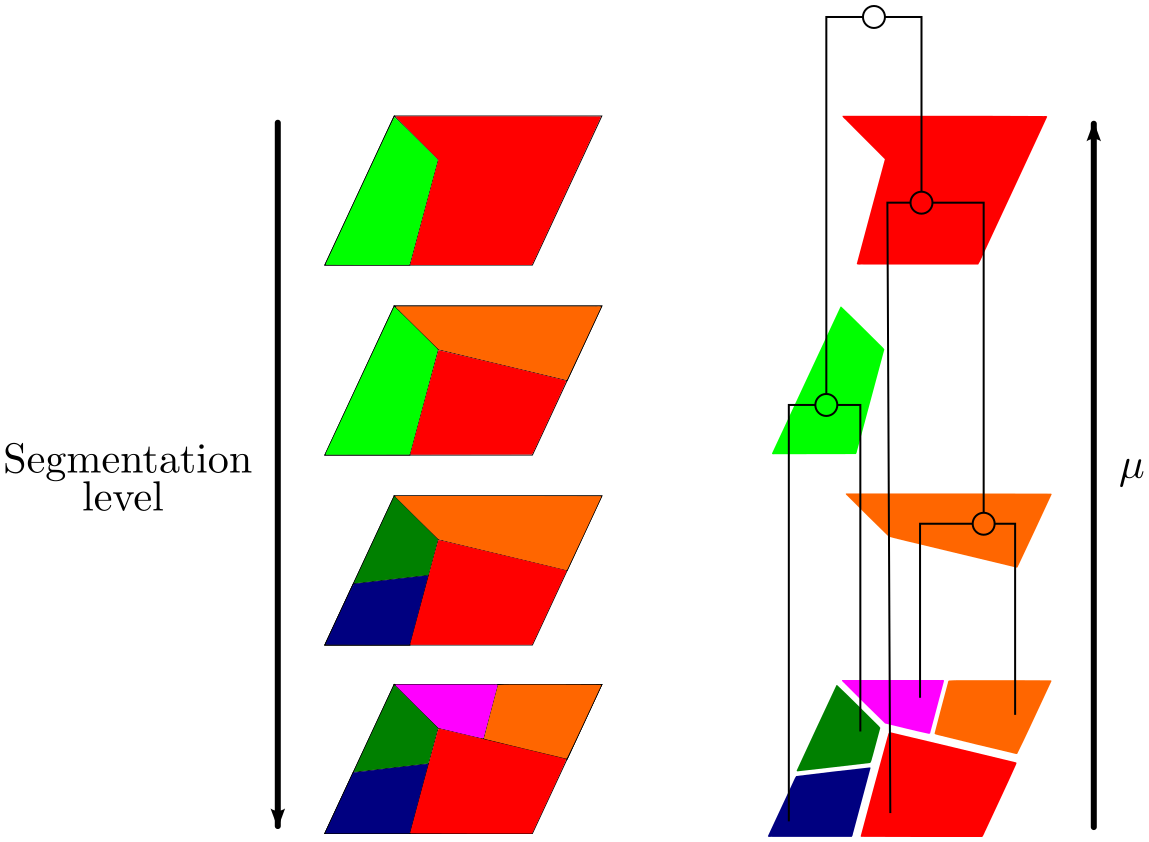
\includegraphics[width=0.5\textwidht]{Figures/seg_hierar}
%\end{figurethesis}

\begin{figurethesis}{test}
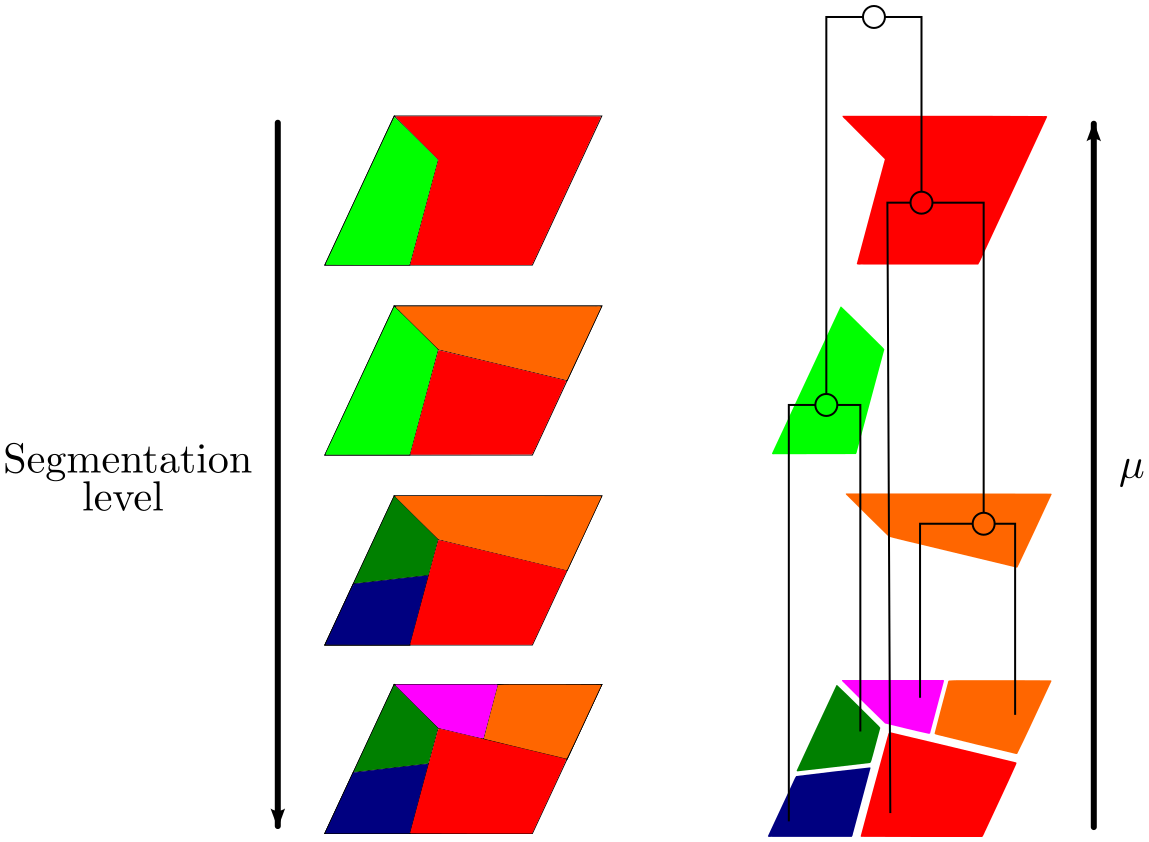
\includegraphics[width=0.75\textwidth]{Figures/seg_hierar}
\caption{Graphical depiction of concepts related to hierarchical segmentation. The diagram on the left shows partitions of an image at four different scales $\mu$. The partition at the top has the highest $\mu$ and is therefore the coarsest, the partition at the bottom is the finest.}
\label{fig:seg_hierar}
\end{figurethesis}


\subsection{Superpixels methods}
Several superpixels algorithms have been developed \citep{achanta2012slic}. They group pixels into perceptually meaningful atomic regions. Many traditional segmentation algorithms have been employed with more or less success to generate superpixels \citep{shi2000normalized, felzenszwalb2004efficient, comaniciu2002mean, vedaldi2008quick, vincent1991watersheds}. These algorithms produce satisfactory results, however, they may be relatively slow and the number, size and shape of the superpixels might not be specified. \\

Superpixels algorithms have then been developed. One can control the number of superpixel, their size and their shape. \cite{moore2008superpixel} creates superpixels based on a grid. Optimal path are found using graph cut methods. \cite{veksler2010superpixels} proposes a generation of superpixels based on a global optimization. They are obtained by stitching together overlapping image patches such that each pixel belongs to only one of the overlapping regions. \cite{levinshtein2009turbopixels} generate superpixels by a dilatation of a set of seed locations using level-set geometric flow. Resulting superpixels are constrained to have uniform size, compactness, and boundary adherence. Finally, \cite{achanta2012slic} proposes a generation of superpixels based on the k-means algorithms. A weighted distance that combines color and spatial proximity is introduced in order to control the size and the compactness of the superpixels.


\subsection{Segmentation of point cloud}
The segmentation of point cloud has been highly assessed \citep{nguyen20133d}. The aim is to extract meaningful objects. Such extraction has two principal objectives:
\begin{itemize}
\item Objects are detected so as to ease or strengthen subsequent classification task. A precise extraction is not mandatory since the labels would be refined after.
\item Objects are precisely delineated in order to derive features from these objects. A high spatial resolution is therefore expected.
\end{itemize}

In forested areas, the only reliable objects to extract are trees. The first way to extract trees from lidar data is to rasterize the point cloud and use image-based segmentation techniques to obtain trees. Several methods have been developed for single tree delineation \citep{dalponte2014tree, vega2014ptrees, kandare2014new}. 

\section{Classification}
A classification is a process that aims to categorize observation. The idea is to assign an observation to one or more classes. This can be done manually or automatically. The classification can be unsupervised, the classes need to be learned and the observation assigned. Such classification is similar to segmentation (see section \ref{sec:C1_seg}). The classification can be supervised, the target classes are known and observations with labels are available.

\subsection{Supervised classification}
A great number of supervised classification algorithms have been developed and used for remote sensing issues \citep{landgrebe2005signal, lu2007survey, mather2016classification}. There are two kind of algorithms: the parametric (or generative) and the non-parametric (or discriminative) methods.

The parametric method assume that each class follow a specific distribution (mainly gaussian). The parameters of the distribution are estimated using the learning set. This is the case for the maximum likelihood \citep{strahler1980use}, maximum a posteriori \citep{fauvel2015fast} or in \cite{trias2005high}.

The non parametric methods do not make any assumption on the classes distribution. In this category of algorithms, the most popular are the Support Vector Machines (SVM) \citep{boser1992training, scholkopf2001learning} and the Random Forest (RF) \citep{breiman2001random}. The artificial neural networks are also efficient algorithms \citep{hepner1990artificial, atkinson1997mapping}. However, despite their great performance in terms of accuracy, they have several drawbacks: firstly, the training process is time consuming and good GPU cards or specific architectures are required in order to reach decent training times \citep{dean2012large, moritz2015sparknet}. Secondly, it requires an important amount of training data in order to correctly optimize the large number of parameters (e.g., hundred of millions). Simpler methods exist, such as the k-nearest neighbor \citep{indyk1998approximate} or the decision trees \citep{breiman1984classification}. The non parametric methods are more efficient  for the discrimination of complex classes \citep{paola1995review, foody2002status}, and are considered as a basis for land cover classification \citep{camps2009kernel}.

We chose to use the RF, which besides their widespread use, since they also offer the possibility of obtaining the probability of belonging of a pixel to a class. This posterior probabilities can be then integrated into a smoothing process. They also report good results, similar to SVM (see Chapter~\ref{Chapter3}). The RF are described in section~\ref{sec:RF}.

\subsection{Random Forest}
\label{sec:RF}
The RF have been introduced by \cite{breiman2001random} and are defined by the aggregation of predictors (decision trees). Here, we refer to the RF with random inputs proposed in \cite{breiman2001random}.

The idea is to create an ensemble of samples $\mathcal{S}_{n}^{\Theta_{1}}$, ..., $\mathcal{S}_{n}^{\Theta_{k}}$ from an initial training set. A Classification and Regression Tree (CART) \citep{breiman1984classification} is built on each sample $\mathcal{S}_{n}^{\Theta_{i}}$. Each tree is built using a a random pool of $m$ features among the $M$ available features. The final classification is obtained by majority vote; each tree votes for a class and the class reaching the most votes wins (see Figure \ref{fig:RF_method}). This algorithm has two parameters: the number of trees $k$ and the number of features $m$ used to build a tree. The first parameter is arbitrary fixed to a high value. The second is generally fixed to the square root of the total number of feature \citep{gislason2006random}.

\begin{figure}[htbp]
\begin{center}
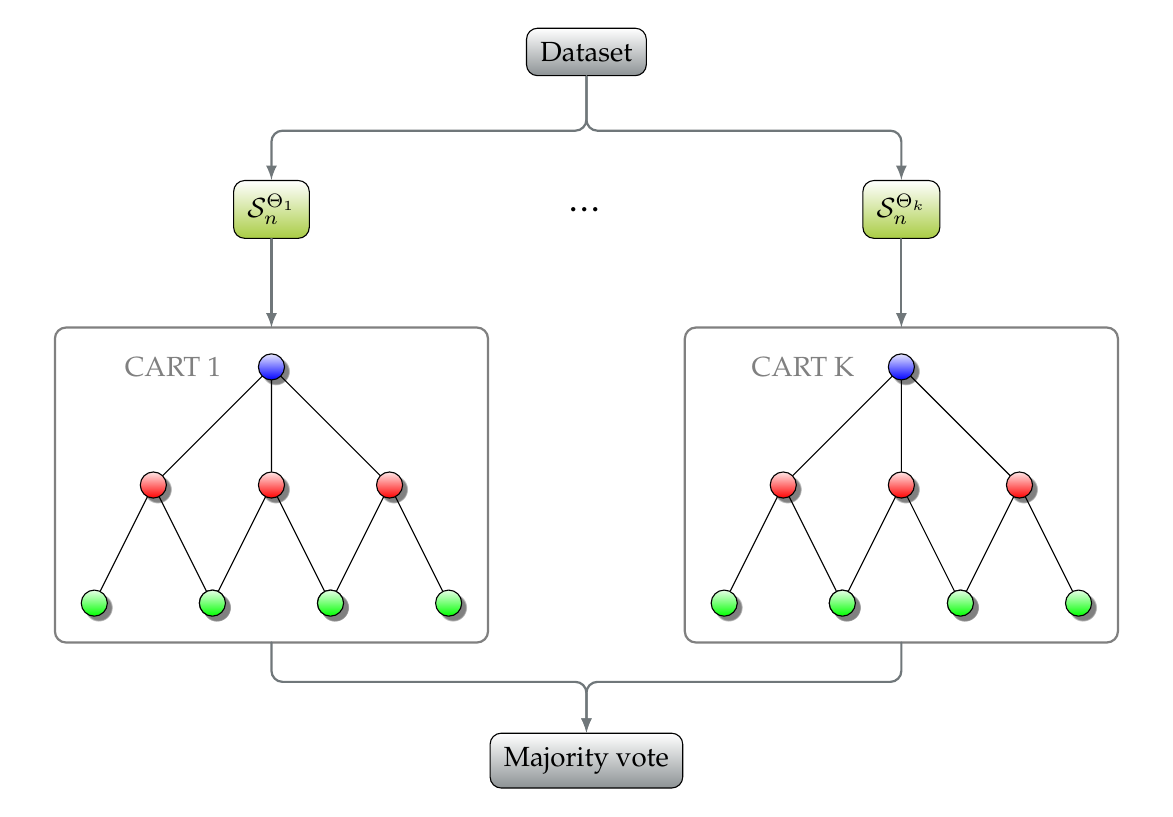
\begin{tikzpicture}
	[shape=circle,cap=round,scale=1]
	%
	\draw (0,2.5)  node[myNodeIGNGris] (data) {Dataset};
	\draw (-4,0.5)  node[myNodeIGNVert] (bootstrap1) {$\mathcal{S}_n^{\Theta_1}$};
	\node (ldots) at (0,0.5) {\textbf{\ldots}};
	\draw (4,0.5) node[myNodeIGNVert] (bootstrapN) {$\mathcal{S}_n^{\Theta_k}$};	
	
	\draw[thick,color=gray,rounded corners](-6.75,-5)--(-6.75,-1)--(-1.25,-1)--(-1.25,-5)--cycle;
	\node[color=gray] at (-5.25,-1.5) {CART 1};
	\node (first tree) at (-4,-3) {\tikz{%
	\node[draw,top color=blue!10,bottom color=blue,minimum size=6pt,circular drop shadow] {} 
	 child  foreach \A in {red,red,red}{  
	   node[draw,top color=\A!10,bottom color=\A,minimum size=4pt,circular drop shadow] {} 
	     child foreach \B in {green,green}{
	       node[draw,top color=\B!10,bottom color=\B,minimum size=3pt,circular drop shadow] {} 
	    }%
	 };%
	}};%
	
	\draw[thick,color=gray,rounded corners](1.25,-5)--(1.25,-1)--(6.75,-1)--(6.75,-5)--cycle;
	\node[color=gray] (cartk) at (2.75,-1.5) {CART K};
	\node (second tree) at (4,-3) {\tikz{%
	\node[draw,top color=blue!10,bottom color=blue,minimum size=6pt,circular drop shadow] {} 
	 child  foreach \A in {red,red,red}{  
	   node[draw,top color=\A!10,bottom color=\A,minimum size=4pt,circular drop shadow] {} 
	     child foreach \B in {green,green}{
	       node[draw,top color=\B!10,bottom color=\B,minimum size=3pt,circular drop shadow] {} 
	    }
	 };
	}};
	
	\draw (0,-6.5)  node[myNodeIGNGris] (vote) {Majority vote};
	
	\draw[myArrowIGNGris] (data.south) -- (0,1.5) -- (-4,1.5)  -- (bootstrap1.north);
	\draw[myArrowIGNGris] (data.south) -- (0,1.5) -- (4,1.5)  -- (bootstrapN.north);
	
	\draw[myArrowIGNGris] (bootstrap1.south) -- (-4,-1);
	\draw[myArrowIGNGris] (bootstrapN.south) -- (4,-1);
	
	\draw[myArrowIGNGris] (-4,-5) -- (-4,-5.5) -- (0,-5.5)  -- (vote.north);
	\draw[myArrowIGNGris] (4,-5) -- (4,-5.5) -- (0,-5.5)  -- (vote.north);

\end{tikzpicture}
\end{center}
\caption{General diagram of the operation of the Random Forest}
\label{fig:RF_method}
\end{figure}


RF have shown better classification performances than traditional Boosting methods \citep{breiman2001random} or SVM \citep{pal2005random}. They are also able to handle big dataset with large number of feature. Furthermore, a measure of feature importance have been introduced in \cite{breiman2001random}. It allows to qualify the relevance of the feature in the classification process \citep{strobl2007bias}.

The importance of a feature $\mathbf{X}_{j}$, $j\in\{1,...,q\}$ (with $q$ the number of feature) is defined as follow. Let $\mathcal{S}_{n}^{\Theta_{i}}$ be a ensemble of sample and $OOB_{i}$ all the observations that does not belong to $\mathcal{S}_{n}^{\Theta_{i}}$. $errOOB_{i}$, the error on $OOB_{i}$ using $\mathcal{S}_{n}^{\Theta_{i}}$, is then computed. A random permutation on the value of the $j^{\text{th}}$ feature of $OOB_{i}$ is performed in order to obtain $\widetilde{OOB_{i}}^j$. $err\widetilde{OOB_{i}^{j}}$ is then computed. The importance of the feature $j$, $FI(\mathbf{X_{j}})$ is the mean of the difference of the errors (see Equation \ref{eq:FI}).

\begin{equation}
\label{eq:FI}
FI(\mathbf{X_{j}})=\frac{1}{k}\sum_{i=1}^{k}(err\widetilde{OOB_{i}^{j}}-errOOB_{i})
\end{equation}
where $k$ is the number of CART.


\section{Dimension reduction and feature selection}
It is possible to derive a lot a features from the original data. All the features are used for the classification. The feature selection methods try to overcome the curse of high dimensionality \citep{bellman2015adaptive, hughes1968mean}. Indeed, the increasing number of features available tends to decrease the accuracy of the classifiers. Furthermore, the computation times increase with the number of features. Thus, reducing the feature dimension is beneficial for the classification task.

Two kind of approaches exist: first the ones based on the extraction of new features summarizing the information by the transformation of the data, generally using a projection in a space of lower dimensionality. Secondly, feature selection approaches that aim to search for an optimal subset of the features.

\subsection{Dimension reduction: feature extraction}
The most popular dimension reduction method is the Principal Component Analysis (PCA). It is an unsupervised method that aim to maximize the variance between data \citep{jolliffe2011principal}. However, it has been demonstrated that PCA is not optimal for the purpose of classification \citep{cheriyadat2003principal}. Other methods have been developed based on the PCA: the Independent Component Analysis (ICA) \citep{jutten1991blind} maximizes the statistical independence between data, and the Maximum Autocorrelation Factor (MAF) \citep{larsen2002decomposition} maximizes the spatial auto-correlation. When training samples are available, supervised methods exist, such as the linear discriminant analysis (LDA) that tries to maximize both the intra-class homogeneity and the inter-class variance \citep{fisher1936use, lebart1997multidimensional}.

\subsection{Feature selection}
Feature selection aims to search for an optimal subset of features without modifying them. To obtain such subset, one can explore the subsets of features or define a criteria to evaluate the subsets. Furthermore, the selection can be supervised or unsupervised. The first aims to discriminate the better the classes while the second are looking for an optimal subset that contains the most informative and less redundant features.
Many exploration methods for feature selection have been proposed in the literature. The naive exhaustive exploration of all the subsets can be envisaged when the number of features is not important. 

\subsubsection{Existing methods}
The feature selection methods can be separated into 3 categories: filters, wrapper and embedded. Within the filter methods, one can distinguish the supervised and unsupervised case depending on whether the notion of classes is taken into account or not.

\paragraph{\underline{$\bullet$ Filters} \\}
The filters methods use a feature selection criteria independent from the classifier. They consider the features according to their capacity to bring together elements of the same class and separate the different elements \citep{john1997enhancements} Thus, these methods compute an individual importance score for each feature, classify the features according to this score and keep only the best. Such scores can be computed using training sample or not. Such methods are independent from a classifier and are used as preliminary step to classification. When training samples are available, separability measures (e.g., Fisher \citep{fisher1936use}, Bhattacharrya or Jeffires-Matusia) allow to determine whether a feature or a subset of feature is well adapted to discriminate the classes \citep{bruzzone2000technique, herold2003spectral, de2005band, serpico2007extraction}. Statistical measures derived from information theory such as the divergence, the entropy or the mutual information have been proposed in the unsupervised case \citep{martinez2007clustering, le2011constrained} or supervised case \citep{battiti1994using, guo2008fast, estevez2009normalized, sotoca2010supervised, cang2012mutual}.
To summarize, criteria for filter selection methods are numerous and cover different approaches. The supervised ones, which sort features according to an individual importance score and retain only the $n$ best remain limited since they do not take into account the dependencies between the selected features. Approaches that directly associate relevance scores with feature sets are more interesting. A distinction is made between supervised and unsupervised approaches. The unsupervised criteria are interesting, but present a risk of selecting attributes that would not all also be useful for classification.

\paragraph{\underline{$\bullet$ Wrapper} \\}
The wrapper methods weight the features according to their pertinence for the prediction \citep{kohavi1997wrappers}. This weighting is related to the performance of a classifier.  \cite{estevez2009normalized, li2011effective, yang2007research, zhuo2008genetic} propose approaches with SVM classifiers. \cite{zhang2007dimensionality, fauvel2015fast} use maximum likelihood classifiers. The RF is also employed in \cite{diaz2006gene}. Data are separated into two subset. The first is used for the training, while the second for the evaluation. The use of a classifier is a big advantage as it fits more to the envisaged problem but can lead to overfitting. However, the use of a classifier significantly increases the computation times. Furthermore, worse results could be obtained when using a feature subset with an other classifier.

\paragraph{\underline{$\bullet$ Embedded} \\}
Eventually, the embedded methods also involve a classifier and select the features during the training process \citep{tang2014feature}. They have two advantages: since they use the data as training, they are robust. Furthermore, the feature selection and the classification are performed together, thus, they are faster than the wrapper methods. Many methods have been proposed. The RF allow to assess the feature importance \citep{breiman2001random} an is also natively embedded since the irrelevant features will not be used in the classification process. Other methods are based on the SVM classifiers, the SVM-RFE (Recursive Feature Elimination) \citep{tuia2009classification} recursively removes the less pertinent features according to a weight estimated with a SVM.

\subsubsection{Optimize the selection}
The set of possible solutions is generally too large to be visited entirely. Thus, using heuristic rules allows to find a solution close enough to the optimal solution while visiting only a reasonable number of configurations. These optimization methods can generally be distinguished in sequential or incremental methods and stochastic methods.

\paragraph{\underline{$\bullet$ Sequential approaches} \\}
The first idea is to add features step by step (forward approaches), also called Sequential Forward Selection (SFS) \citep{marill1963effectiveness}. It could also be methods that start from the entire feature set and remove feature step by step (backward approaches), also called Sequential Backward Selection (SBS) \citep{whitney1971direct}. A generalization of these methods have been proposed in \cite{kittler1978feature}. Finally, the forward and backward methods could be combined in order to improve the process. The Sequential Floating Forward Selection (SFFS) and the Sequential Floating Backward Selection (SFBS) \citep{pudil1994floating} propose such improvement. \\

\paragraph{\underline{$\bullet$ Stochastic approaches} \\}
Stochastic algorithms will involve hazard in their exploration of the space of solutions. The random initialization and search for a solution can therefore propose different solutions of equivalent quality from a single dataset.
The generation of the subset can be totally random \citep{liu1997feature}. Genetic algorithms propose a ponderation of the subsets according to their importance \citep{goldberg1989genetic}. They allow a faster convergence to a more stable solution. The Particle Swarm Optimization (PSO) algorithm \citep{yang2007research}  is also a fast and select relevant features. For finding an approximate optimal subset of features,  simulated annealing \citep{de2005band, chang2011parallel}. \\

\section{Smoothing methods}
Pixel-wise classification is not sufficient for both accurate and smooth land-cover mapping with VHR remote sensing data. This is particularly true in forested areas: the large intra-class and low inter-class variabilities of classes result in noisy label maps at pixel or tree levels. This is why various regularization solutions can be adopted from the literature (from simple smoothing to probabilistic graphical models).\\
According to \cite{schindler2012overview}, both local and global methods can provide a regularization framework, with their own advantages and drawbacks.

\subsection{Local methods}
In local methods, the neighborhood of each element is analyzed by a filtering technique. The labels of the neighboring pixels (or the posterior class probabilities) are combined so as to derive a new label for the central pixel. Majority voting, Gaussian and bilateral filtering can be employed if it is not targeted to smooth class edges. The majority vote can also be used when a segmentation is available: the majority class is assigned to the segment.\\
The probabilistic relaxation is an other local smoothing method that aims at homogenizing probabilities of a pixel according to its neighboring pixels. The relaxation is an iterative algorithm in which the probability at each pixel is updated at each iteration in order to have it closer to the probabilities of its neighbors \citep{Gong198933}. It reports good accuracies with decent computing time and offers an alternative to edge aware/gradient-based techniques that may not be adapted in semantically unstructured environments.

\subsection{Global methods}
Global methods consider the full area of interest at the same time. They are based on Markov Random Fields (MRF, see Figure~\ref{fig:graph_cut}), the labels at different locations are not considered to be independent. The optimal configuration of labels is retrieved when finding the Maximum A Posteriori over the entire field \cite{Gab_MRF}. The problem is therefore considered as the minimization procedure of an energy $E$ over the full image $I$. Despite a simple neighborhood encoding (pairwise relations are often preferred), the optimization procedure propagates over large distances. Depending on the formulation of the energy, the global minimum may be reachable. However, a large range of optimization techniques allow to reach local minima close to the real solution, in particular for random fields with pairwise terms \cite{kolmogorov2004energy}. For genuine structured predictions, in the family of graphical probabilistic models, Conditional Random Fields (CRF, see Figure~\ref{fig:graph_cut}) have been massively adopted during the last decade. Interactions between neighboring objects, and subsequently the local context can be modeled and learned. In particular, Discriminative Random Fields (DRF, \cite{DRF}) are CRF defined over 2D regular grids, and both unary/association and binary/interaction potentials are based on labeling procedure outputs. Many techniques extending this concept or focusing on the learning or inference steps have been proposed in the literature \cite{ijcv_kohli09,Ladicky2012}. A very recent trend even consists in jointly considering CRF and deep-learning techniques for the labeling task \cite{CNN_CRF}.\\

\begin{figure}[htbp]
\begin{center}
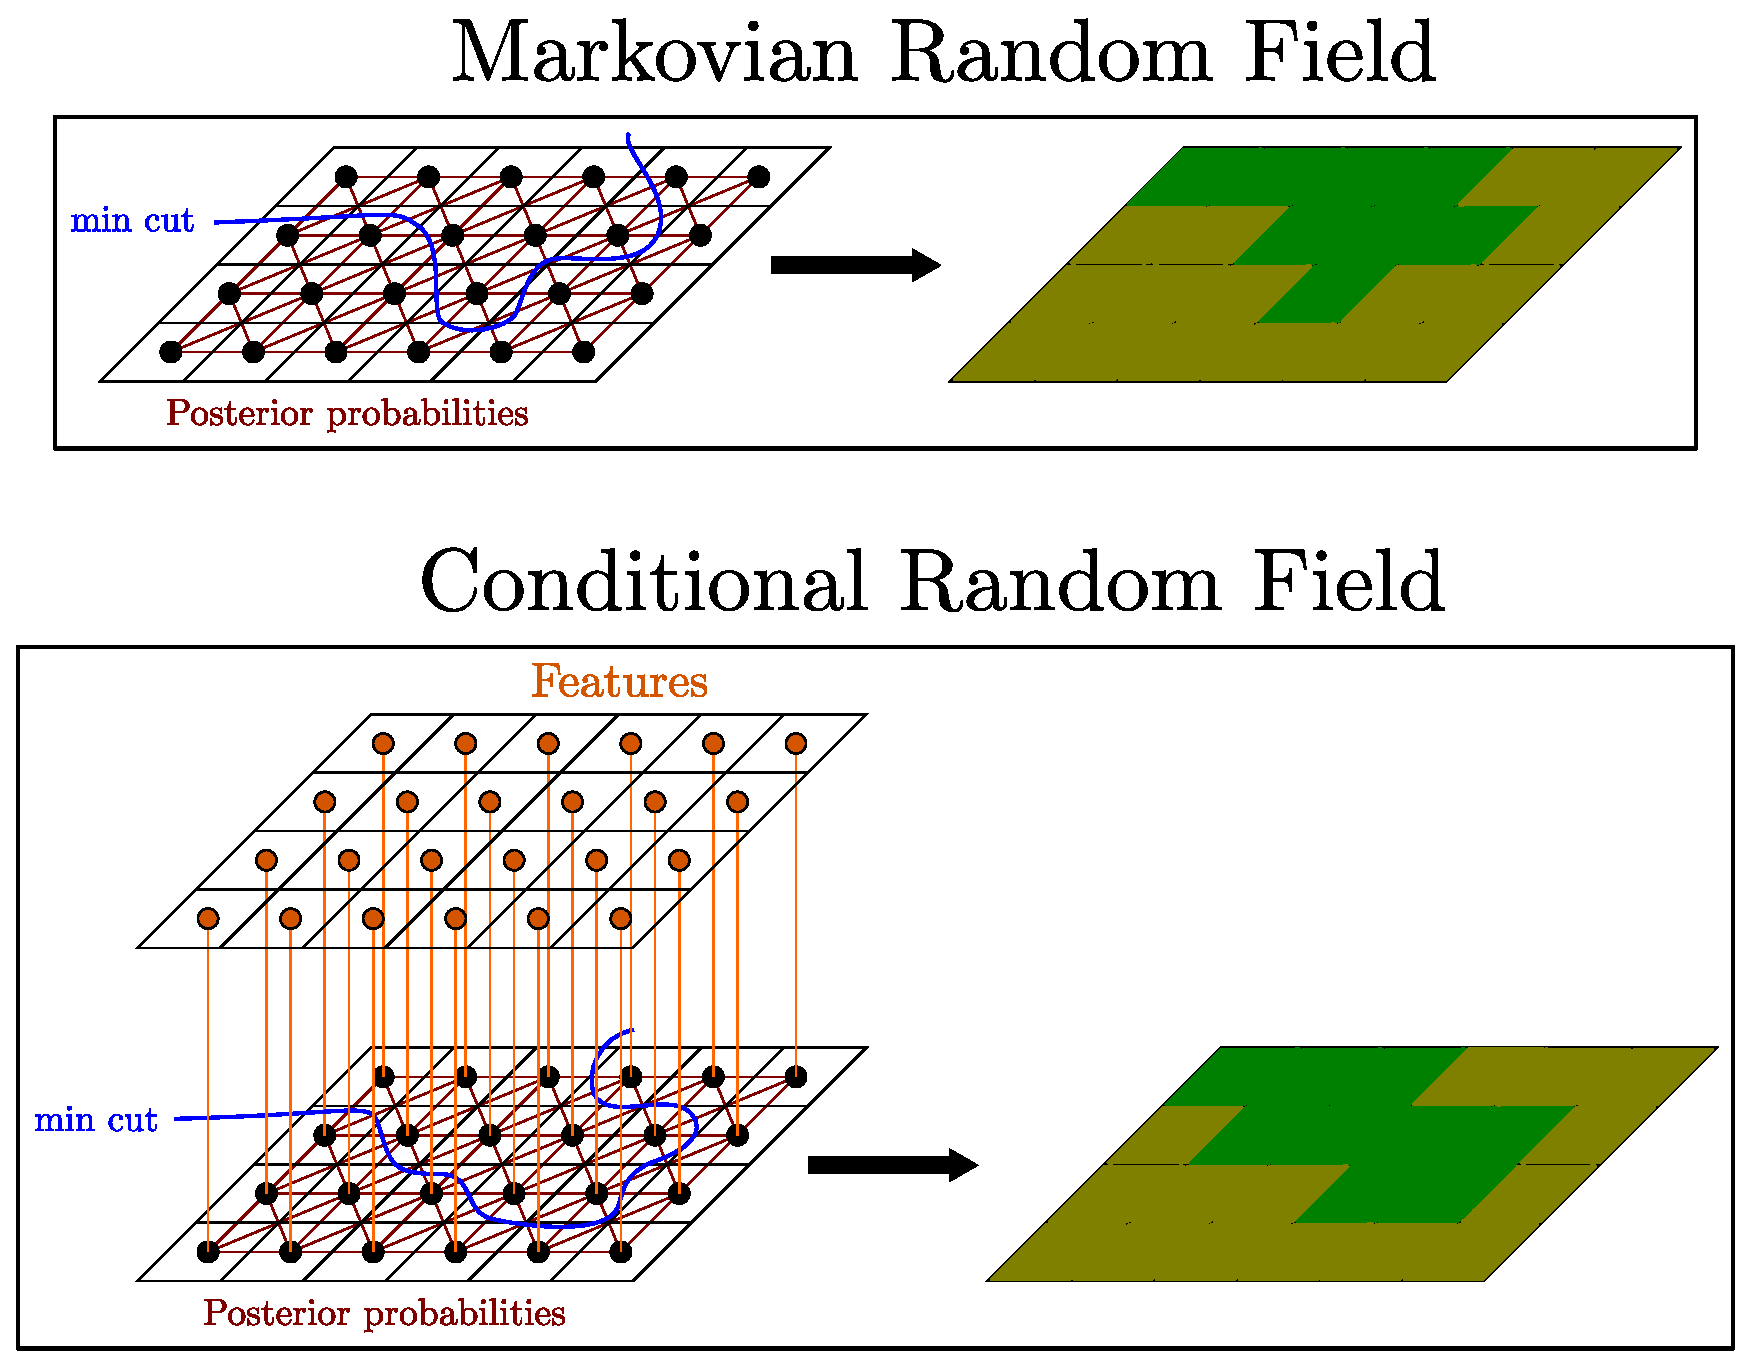
\includegraphics[width=\textwidth]{Figures/graph_cut}
\caption{8-connected MRF and CRF. The MRF only take into account the posterior probabilities to compute the graph, while CRF also include contextual information (the features).}
\label{fig:graph_cut}
\end{center}
\end{figure}

In standard LC classification tasks, global methods are known to provide significantly more accurate results \cite{schindler2012overview} since contextual knowledge is integrated. This is all the more true for VHR remote sensing data, especially in case of a large number of classes (e.g., 10, \cite{isprs-archives-XLI-B4-11-2016}), but presents two disadvantages. For large datasets, their learning and inference steps are expensive to compute. Furthermore, parameters should often be carefully chosen for optimal performance, and authors that managed to alleviate the latter problem still report a significant computation cost \cite{Lucchi_ICCV2011}.

\stopcontents[chapters]


\openchapter
% Chapter 2

\chapter{Method} % Main chapter title
\label{Chapter2} % For referencing the chapter elsewhere, use \ref{Chapter1} 

\startcontents[chapters]
\Mprintcontents


%----------------------------------------------------------------------------------------

% Define some commands to keep the formatting separated from the content 
%\newcommand{\keyword}[1]{\textbf{#1}}
%\newcommand{\tabhead}[1]{\textbf{#1}}
%\newcommand{\code}[1]{\texttt{#1}}
%\newcommand{\file}[1]{\texttt{\bfseries#1}}
%\newcommand{\option}[1]{\texttt{\itshape#1}}

%----------------------------------------------------------------------------------------

\section{General flowchart}

With respect to the methods mentioned above, it appears that there are no forest stand segmentation method, based on tree species, that can satisfactorily handle a large number of classes ($>$5). The proposed framework is a fully automatic and modular method for species-based forest stand segmentation. The method is composed of four main steps; over-segmentation feature computation, vegetation type (mainly tree species) classification and regularization (see Figure \ref{fig:flowchart}).

\begin{figure}
\includegraphics[width=\textwidth]{Figures/method.eps}
\caption{Flowchart of the proposed method.}
\label{fig:flowchart}
\end{figure}

Features are first derived at the pixel and at the object level. The most relevant ones are subsequently selected in a supervised way. The objects are extracted using various segmentation methods, since they appear to be sufficient for subsequent steps. A classification is performed at the object level as it significantly improves the discrimination results (about $10\%$ better than the pixel-based approach). This classification is then smoothed. The smoothing may produce homogeneous vegetation type (mainly tree species) areas with smooth borders. The contributions of this method are two-fold:
\begin{itemize}
\item Such framework can be fed with specific constraints allowing to tailor the results to specific criteria (height, age, specie, maturity, density,~\ldots).
\item Here, the training set is automatically derived from an existing forest land-cover geodatabase. Specific attention is paid to the extraction of the most relevant training pixels, which is highly challenging with outdated and generalized vector databases.
\end{itemize}

\section{Over-segmentation}
The over-segmentation aims to extract small object that are consistent according to the input data. They are detected so as to ease or strengthen subsequent classification task. A precise extraction is not mandatory since the labels would be refined after.

\subsection{Segmentation of lidar data}
Two approaches could be envisaged: the direct segmentation of the point cloud or the segmentation of a rasterized lidar feature using image-based segmentation algorithms. \\

The tree extraction from the point cloud is a complex task that has been widely discussed \citep{dalponte2014tree, vega2014ptrees, kandare2014new}. However, a precise tree extraction is not needed here, since the extracted trees are only needed to improve the classification task. A coarse method is therefore adopted: the tree tops are first extracted from the lidar point clouds using a local maximum filter. A point is considered as a tree top when it has the highest height value within a 5 meter radius. Only the points above 3$\:$meters are retained as it is a common threshold of the literature \citep{eysn2012forest}, and appears to be highly discriminative in non-urban areas. Points belonging to a tree are obtained through two criteria. (i) If the height of a point within a 5$\:$m radius is greater or equal than 80\% the height of the closest tree top, it is aggregated to the tree top. (ii) If the distance in the  $(x,y)$ plane between an unlabeled point and the closest tree point is smaller than 3$\:$m  they are also aggregated. This delineation method allows to discard low vegetation, but buildings might be extracted and considered as trees. \\

The image-based segmentation are also very efficient for the over-segmentation of lidar data. They are mainly applied on the normalized digital surface model (height). Thus a method using a single band is needed. The watershed algorithm \citep{vincent1991watersheds} with specific parameters allow to obtain quickly a consistent over-segmentation of the image. A hierarchical segmentation \citep{guigues2006scale} is more adapted since only one parameter that control the segmentation level needs to be provided.

\subsection{Segmentation of optical images}
Several algorithms have been developed for the over-segmentation of optical RGB (Red-Green-Blue) images. The most common are the superpixels methods \citep{achanta2012slic}.

\section{Feature extraction}
\subsection{Point-based lidar features.}
Lidar-derived features require a consistent neighborhood for their computation. For each lidar point, 3 cylindrical neighborhoods, aligned with the vertical axis, are used (1$\:$m, 3$\:$m and 5$\:$m radii, infinite height). A cylinder appears to be the most relevant environment in forested areas so as to take into account the variance of altitudes of the lidar points. Three radius values are considered so as to handle the various sizes of the trees and assuming a feature selection step will prune the initial set of attributes. {Two vegetation density features, $\mathcal{D}_{1}$ and $\mathcal{D}_{2}$, are computed: the first one based on the number of local maxima within the neighborhoods, and the second one related to the number of non-ground points within the neighborhoods (ground points were previously determined by a filtering step). $\mathcal{D}_{1}$ and $\mathcal{D}_{2}$ are calculated as follows:
\begin{eqnarray}
\mathcal{D}_{1} & = & \sum_{r_{1} \in \{1,3,5\}}\sum_{r_{2} \in \{1,3,5\}}Nt_{r_{1},r_{2}}, \\
\mathcal{D}_{2} & = & \frac{1}{3}\sum_{r \in \{1,3,5\}}\frac{Ns_{r}}{Ntot_{r}},
\end{eqnarray}
where $Nt_{r_{1},r_{2}}$ is the number of local maxima retrieved from a $r_{1}$ maximum filter within the cylindrical neighborhood of radius $r_{2}$. $Ns_{r}$ is the number of points classified as ground points within the cylindrical neighborhood of radius $r$ and $Ntot_{r}$ is the total number of points within the cylindrical neighborhood of radius $r$.} Additionally, the scatter $\mathcal{S}$ and the planarity $\mathcal{P}$ features are computed following \citet{Weinmann2015286}:
\begin{eqnarray}
\mathcal{S} & = & \frac{1}{3}\sum_{r \in \{1,3,5\}}\frac{\lambda_{3,r}}{\lambda_{1,r}}, \\
\mathcal{P} & = & \frac{1}{3}\sum_{r \in \{1,3,5\}}2\times(\lambda_{2,r}-\lambda_{3,r}),
\end{eqnarray}
where $\lambda_{1,r}\geq\lambda_{2,r}\geq\lambda_{3,r}$ are the eigenvalues of the covariance matrix within the cylindrical neighborhood of radius $r$. They are retrieved with a standard Principal Component Analysis. \\
Statistical features, known to be relevant for vegetation type (mainly tree species) classification \citep{dalponte2014tree,torabzadeh2015optimal}, are also derived. For each lidar point, the same 3 cylindrical neighborhoods are used. Two basic information from the lidar data, namely height and intensity, are used to derive statistical features. A statistical feature $f_{d}$, derived from an original feature $f_{o}$, (height or intensity) is computed as follows: \\
\begin{equation}
f_{d} = \frac{1}{3}\sum_{r \in \{1,3,5\}}f_{s}(\mathbf{p_{r,f_{o}}}), 
\label{eq:derive_features}
\end{equation}
where $f_{s}$ is a statistical function (minimum; maximum; mean; median; standard deviation; median absolute deviation from median (medADmed); mean absolute deviation from median (meanADmed); skewness; kurtosis; 10$^{\text{th}}$, 20$^{\text{th}}$, 30$^{\text{th}}$, 40$^{\text{th}}$, 50$^{\text{th}}$, 60$^{\text{th}}$, 70$^{\text{th}}$, 80$^{\text{th}}$, 90$^{\text{th}}$ and 95$^{\text{th}}$ percentiles), and $\mathbf{p_{r,f_{o}}}$ a vector containing the sorted values of the original feature $f_{o}$ within the cylindrical neighborhoods of radius~$r$. All the statistical functions are used for the height. Only the mean is used for the intensity: it is hard to know how well the sensor is calibrated and a suitable correction of intensity values within tree canopies has not yet been proposed. \\
24 features are extracted during this step; 2 related to vegetation density, 2 related to the 3D local distribution of the point cloud (planarity and scatter), and 20 statistical features.

\subsection{Pixel-based multispectral features.}
The original 4 spectral bands of the image are kept and considered as multispectral features. The Normalized Difference Vegetation Index (NDVI), \citep{tucker1979red},
the Difference Vegetation Index (DVI), \citep{bacour2006normalization}
and the Ratio Vegetation Index (RVI) \citep{jordan1969derivation}
are computed as they are relevant vegetation indices. Indeed, they can provide more information about the species than the original bands alone \citep{zargar2011review}. As the point-based lidar features, statistical features are also derived from each band and each vegetation index according to Equation~\ref{eq:derive_features} (3 circular neighborhoods of 1$\:$m, 3$\:$m and 5$\:$m radii). Other statistical functions are used (minimum; maximum; mean; median; standard deviation; mean absolute deviation from median (meanADmed); mean absolute deviation from mean (meanADmean); median absolute deviation from median (medADmed); median absolute deviation from mean (medADmean). Finally, the pixel-based multispectral feature set is composed of 70 attributes.

\subsection{Pixel-based lidar features.}
The lidar features are rasterized at the same resolution of the multispectral image using a pit-free method proposed in \citep{khosravipour2014generating}. This rasterization method is interesting because it produces smooth images that will lead to better results for classification and regularization \citep{Li2013104}. Such data fusion process at the feature level is valid since both datasets have approximately the same spatial resolution. The Canopy Height Model (CHM) is also computed using this method, at the same spatial resolution using an existing 1$\:$m Digital Terrain Model provided with the filtered point cloud \citep{Ferraz201623}. The CHM is very important as it allows to derive the height above the ground and is known as a very discriminative feature for classification \citep{Mallet2011S71,Martin}.

\subsection{Object-based feature map.}
The pixel-based multispectral and lidar maps are merged so as to obtain a pixel-based feature map. Then, an object-based feature map is created using the over-segmentation and the pixel-based feature map. The value $v_{t}$ of a pixel belonging to an object $t$ in the object-based feature map is computed as follows:
\begin{equation}
v_{t}=\frac{1}{N_{t}}\sum_{p \in t} v_{p},
\end{equation}
where $N_{t}$ is the number of pixels in object $t$ ,and $v_{p}$ is the value of the pixel $p$.
If a pixel does not belong to a tree, it keeps the value of the pixel-based feature map. Here, only the mean value of the pixels within the tree is envisaged but one can also consider other statistical values (minimum, maximum, percentiles etc.). \\
Other morphological features could also be directly derived from the lidar cloud point at the object-level. For instance, an alpha-shape can be performed on the individual trees \citep{vauhkonen2010imputation} and a penetration feature can be derived as it can help to classify vegetation type (mainly tree species). However, low point densities (1-5 points/m$^{2}$) compatible with large-scale lidar surveys are not sufficient in order to derive a significant penetration indicator.

\section{Classification}
The classification is performed using a supervised classifier, in order to discriminate the vegetation type (mainly tree species) provided by an existing forest land-cover database. The classifier used in this study is the Random Forest (RF), implemented in OpenCV \citep{opencv}, as it has been shown relevant in the literature \citep{belgiu2016random} and in a previous study compared to SVM \citep{dechesne2016forest}, since it provide similar results while being faster. The outputs of the classification are (i) label map and (ii) probability map (posterior class probabilities for each pixel/object). This probability map is the main input for the subsequent regularization step. \\
In order to reduce the computation times, a feature selection is carried out to identify an "optimal" feature subset. Additionally, a strategy is proposed in order to select the most suitable training pixels for an existing land-cover forest maps, subsequently improving the classification accuracy.

\subsection{Training set design}
Using an existing forest land-cover (LC) database for training a model is not straightforward \citep{isprsannals-II-3-W2-13-2013,rs6053965,isprs-annals-III-7-133-2016}. First, locally it can suffer from a lack of information (not all the classes of interest are present). Secondly, this database may also be semantically and, more frequently, geometrically incorrect (see Figure~\ref{fig:delineation_errors}): changes may have happened (forest cut or grow) and the geodatabase may have been generalized, resulting in sharp polygon vertices that do not exactly correspond to the class borders. Thirdly, in many forest LC databases, polygons of a given vegetation type (mainly tree species) may contain other vegetation type (mainly tree species) in a small proportion. Two strategies are employed to overcome these problems: 

Firstly, in order to increase the knowledge on existing class labels, the model could be trained on a larger area. The size of the training area has been chosen arbitrarily. However, when it is too large, we observe that the quality of the classification decreases. The optimal choice of the training area has not been investigated yet. {The model has therefore been trained on a larger area than the ones of interest}. The areas selected for the training are the ones maximizing the number of classes within a 5$\:$km search zone.

Secondly, in order to correct the potential errors of the LC database, a k-means clustering has been therefore performed on each of the labels in the training area. We assume that erroneous pixels are present in a small proportion and that therefore the main cluster corresponds to the class of interest. Let $p_{i-c,t}$ be the $i^{\text{th}}$ pixel of the vegetation type (mainly tree species) $t$ in the cluster $c$ of the k-means. The pixels $P_{t}$ used to train the model for the vegetation type (mainly tree species) $t$ correspond to the set:
\begin{equation}
P_{t} = \{{p_{i-c,t} \quad | \quad \underset{c \in [1,k]}{c=\text{argmax }}\text{Card} ( \cup_{i} p_{i-c,t} ) } \}.
\end{equation}
That is to say, only samples belonging to the main k-mean cluster among training pixels for one class are kept in the training dataset. \\
In practice, $k=3$: the main cluster corresponds to the label of interest whereas the two other ones correspond to the ground and minority vegetation type (mainly tree species) within the polygons. 1000 samples per class are then randomly selected in order to design the final training set.

\subsubsection{Feature selection}
Due to the high number of features involved, an automatic Feature Selection (FS) has been integrated. This selection is composed of two steps: the choice of the number of features to select and the feature selection itself. Indeed, the choice of the number of features is very important because it enables to greatly decrease the computation times. \\
The Sequential Forward Floating Search (SFFS) \citep{pudil1994floating} algorithm is used for both steps. The SFFS algorithm has two main advantages: (i) it can be used with many classification score (in this study, the Kappa coefficient), (ii) it enables to access to the evolution of the classification score/accuracy according to the number of selected features. The accuracy of the classification is assessed through the Kappa coefficient of the RF classifier. The SFFS algorithm selects $p$ features by maximizing FS score criterion (the Kappa coefficient). In order to retrieve the optimal number of features, the SFFS algorithm is performed $n$ times on different training sets with $p$ equal to the total number of features (95). The classification accuracy is conserved for each selection of $s$ features ($s \in [1, p]$) and averaged over the $n$ iterations. The number of optimal features $n_{\text{opt}}$ corresponds to the size of the selection of $s$ features having the maximal mean accuracy. In order to reduce the computation times, the optimal number of features was computed for a single 1$\:$km$^{2}$ area and used for all the areas of interest. \\
The feature selection is then carried out for each area of interest (one selection for each area) with $p=n_{\text{opt}}$. The selected features are used for both the classification and the energy minimization framework. The feature selection could be carried out only once on a single area or on multiple areas in order to reduce the computation times.

\section{Smoothing}
The proposed method assumes that a label map is provided for the areas of interest, and is accompanied with a class membership probability map, which provides, for each pixel of the image, the posterior class membership for all classes of interest. These are the necessary inputs for all methods described below. In practice, the strategy proposed in \cite{clement_IJPRS} is as followed: a supervised classification is performed on a selection of features extracted both from 3D lidar point clouds and aerial multispectral images. The training pixels are selected according to an existing forest LC geodatabase. The used classifier is the Random Forest (RF) classifier. This is an efficient classifier, that directly handles multiple classes, and provides posterior probabilities for each class.\\
Here, both local and global methods are tested. For local techniques, majority voting and probabilistic relaxation are selected. For global methods, various energy formulations based on a feature-sensitive Potts model are proposed.

\subsection{Local methods}
\subsubsection{Filtering}
An easy way to smooth a probability map is to filter it. All the pixels in a $r \times r$ pixels moving window $\mathcal{W}$ are combined in order to generate an output label of the central pixel. The most popular filter is the majority filter. Firstly, the class probabilities are converted into labels, assuming that the label of pixel $\mathbf{x}$ is the label of the most probable class.\\
\begin{equation}
C(\mathbf{x})=[c_{i}|P(\mathbf{x},c_{i}) \geq P(\mathbf{x},c_{j}) \forall j],
\end{equation}
with $i,j \in [1,n_{c}]$, where $n_{c}$ is the number of classes. From this label image, the final smoothed result is obtained by taking the majority vote in a local neighborhood.
\begin{equation}
C_{smooth}(\mathbf{x})=\underset{i}{\text{arg max}}\left[ \sum_{\mathbf{u}\in\mathcal{W}}\left[C(\mathbf{u})=c_{i}\right] \right].
\end{equation}
Many other filters have been developed.

\subsubsection{Probabilistic relaxation}
The probabilistic relaxation aims at homogenizing probabilities of a pixel according to its neighboring pixels. The relaxation is an iterative algorithm in which the probability at each pixel is updated at each iteration in order to have it closer to the probabilities of its neighbors \cite{Gong198933}. It was adopted for simplicity reasons. First, good accuracies are reported with decent computing time, which is beneficial over large scales. Secondly, it offers an alternative to edge aware/gradient-based techniques that may not be adapted in semantically unstructured environments like forests. The probability $P_{k}^{t}(\mathbf{u})$ of class $k$ at a pixel $\mathbf{u}$ at the iteration $t$ is defined by  $\delta P_{k}^{t}(\mathbf{u})$ which depends on:
\begin{itemize}
\item The distance $d_{\mathbf{u},\mathbf{v}}$ between the pixel $\mathbf{u}$ and its neighbors $\mathbf{v}$ (the pixels that are distant of less than $r$ pixels from $\mathbf{u}$).
\item A co-occurrence matrix $T_{k,l}$ defining a priori correlation between the probabilities of neighboring pixels. The local co-occurrence matrix has been tuned arbitrarily, but can also be estimated using training pixels \cite{VolpiCVPR2015}. The matrix is expressed as follow: \\
$T_{k,l}=\begin{bmatrix}
0.8 & p & \cdots & p \\
p & \ddots & \ddots & \vdots \\
\vdots & \ddots & \ddots & p \\
p & \cdots & p & 0.8
\end{bmatrix}$, with $p=\frac{0.2}{n_{c}-1}$.
\end{itemize}
The update factor is then defined as:
\begin{equation}
\delta P_{k}^{t}(\mathbf{u})=\sum_{\mathbf{v} \in \mathcal{N_{\mathbf{u}}}} d_{\mathbf{u},\mathbf{v}} \sum_{l=1}^{n_{c}} T_{k,l}(\mathbf{u},\mathbf{v}) \times P_{l}^{t}(\mathbf{v}).
\end{equation}
In order to keep the probabilities normalized, the update is performed in two steps using the unnormalized probability $Q_{k}^{t+1}(\mathbf{u})$ of class $k$ at a pixel $\mathbf{u}$ at the iteration $t+1$:
\begin{equation}
Q_{k}^{t+1}(\mathbf{u})=P_{k}^{t}(\mathbf{u}) \times \big(1 + \delta P_{k}^{t}(\mathbf{u})\big),
\end{equation}
\begin{equation}
P_{k}^{t+1}(\mathbf{u})=\frac{Q_{k}^{t+1}(\mathbf{u})}{\sum_{l=1}^{n_{c}}Q_{l}^{t+1}(\mathbf{u})}.
\end{equation}

\subsection{Global smoothing}
The global smoothing method uses only a small number of pairwise cliques between neighboring pixels (4-neighbors or 8-neighbors) to describe the smoothness. Over the entire resulting first order random fields, the maximization of the posterior probability leads to a smoothed results. This can be done by finding the minimum of the negative log-likelihood, $\underset{C}{\text{arg min}}E(I,C,A)$ with
\begin{equation}
\begin{aligned}
& E(I,C,A)=\sum_{\mathbf{u}\in I}E_{\text{data}}(\mathbf{u},P(\mathbf{u})) + \\
& \gamma\sum_{\mathbf{u} \in I, \mathbf{v} \in \mathcal{N}_{\mathbf{u}}} E_{\text{pairwise}}(\mathbf{u}, \mathbf{v}, C(\mathbf{u}), C(\mathbf{v}), A(\mathbf{u}), A(\mathbf{v})),
\end{aligned}
\end{equation}
where $P(\mathbf{u})=[P(\mathbf{u},c_{i})|P(\mathbf{u},c_{i}) \geq P(\mathbf{u},c_{j}) \forall j]$, $A(\mathbf{u})$ are the values of the features at pixel $\mathbf{u}$ (such as height, reflectance...) and $\mathcal{N}_{\mathbf{u}}$ is the 8-connected neighborhood of the pixel $\mathbf{u}$ (only the 8-connected neighborhood is investigated in this paper). When $\gamma=0$, the pairwise term has no effect in the energy formulation; the most probable class is attributed to the pixel, leading to the same result as the classification output. When $\gamma \neq 0$, the resulting label map becomes more homogeneous, and the borders of the segments/stands are smoother. However, if $\gamma$ is too high, the small areas are bound to be merged into larger areas, removing a part of the useful information provided by the classification step. The automatic tuning of the parameter $\gamma$ has been addressed in \cite{Gab_MRF} but is not used here.\\
In this paper, two formulations of $E_{\text{data}}$ (unary term) and four formulations of $E_{\text{pariwise}}$ (prior) are investigated. \\
\subsubsection{Unary term}
A widely used formulation for the unary term is the log-inverse formulation using the natural logarithm. It corresponds to the information content in information theory and is formulated as follow:
\begin{equation}
E_{\text{data}}=-\text{log}(P(\mathbf{u})).
\label{eq:data1}
\end{equation}
It highly penalizes the low-probability classes but increase the complexity with potential infinite values.\\
An other simple formulation for the unary term is the linear formulation,
\begin{equation}
E_{\text{data}}=1-P(\mathbf{u}).
\label{eq:data2}
\end{equation}
It penalizes less than the log-inverse formulation but has the advantage of having values lying in $[0,1]$. \\
\subsubsection{Prior}
In this work, the prior has a value depending on the class of neighboring pixels. In the four formulations, two neighboring pixels pay no penalty if they are assigned to the same class. Two basic and popular priors, the \textit{Potts model} and the \textit{contrast-sensitive Potts model} (called here \textit{z-Potts model}), are investigated. In the \textit{Potts model}, two neighboring pixels pay the same penalty if they are assigned to different labels, the prior for the \textit{Potts model} is:
\begin{equation}
\begin{aligned}
& E_{\text{pairwise}}(C(\mathbf{u}) = C(\mathbf{v}))=0, \\
& E_{\text{pairwise}}(C(\mathbf{u}) \neq C(\mathbf{v}))=1.
\end{aligned}
\label{eq:prior1}
\end{equation}\\
In the \textit{z-Potts model}, the penalty for a change of label depends on the gradient of height between two neighboring pixels. The \textit{z-Potts model} is a standard \textit{contrast-sensitive Potts model} applied to the height obtained from the point clouds. Here, since we are dealing with forest stands that are likely to exhibit distinct heights, the gradient of the height map (given with the 3D lidar point cloud) is computed for each of the four directions separately. The maximum $M_{g}$ over the whole image in the four directions is used to compute the final pairwise energy. A linear function has been used: the penalty is highest when the gradient is 0, and decreases until the gradient reaches its maximum value. The prior of the \textit{z-Potts model} is therefore:
\begin{equation}
\begin{aligned}
& E_{\text{pairwise}}(C(\mathbf{u}) = C(\mathbf{v}))=0, \\
& E_{\text{pairwise}}(C(\mathbf{u}) \neq C(\mathbf{v}))=1-\frac{g_{\mathbf{u} \rightarrow \mathbf{v}}}{M_{g}},
\end{aligned}
\label{eq:prior2}
\end{equation}
where $g_{\mathbf{u} \rightarrow \mathbf{v}}$ is the gradient between pixel $\mathbf{u}$ and pixel $\mathbf{v}$, i.e., the absolute value of the height difference of the two pixels.\\
An other pairwise energy investigated is a global feature sensitive energy (called here \textit{Exponential-features model}). The pairwise energy is computed with respect to a pool of $n$ features. When the features have close values, the penalty is high and decreases when the features tends to be very different. The pairwise energy in this case is expressed as follows:
\begin{equation}
\begin{aligned}
& E_{\text{pairwise}}(C(\mathbf{u}) = C(\mathbf{v}))=0, \\
& E_{\text{pairwise}}(C(\mathbf{u}) \neq C(\mathbf{v}))=\frac{1}{n}\sum_{i=1}^{n}\exp({-|A_{i}(\mathbf{u})-A_{i}(\mathbf{v})|}),
\end{aligned}
\label{eq:prior3}
\end{equation}
where $A_{i}(\mathbf{u})$ is the value of the $i^{\text{th}}$ feature of the pixel $\mathbf{u}$. To compute such energy, the features need to be first normalized (i.e., zero mean, unit standard deviation) in order ensure that they all have the same dynamic.\\
The last formulation investigated is also a global feature sensitive energy (called here \textit{Distance-features model}). The pairwise energy is still computed with respect to a pool of $n$ features. In this case, the energy is computed according to the distance between the two neighboring pixels in the feature space, the penalty is high when the pixels are close in the feature space and decrease when they get distant. The pairwise energy in this case is expressed as follow:
\begin{equation}
\begin{aligned}
& E_{\text{pairwise}}(C(\mathbf{u}) = C(\mathbf{v}))=0, \\
& E_{\text{pairwise}}(C(\mathbf{u}) \neq C(\mathbf{v}))=1-||A(\mathbf{u});A(\mathbf{v})||_{n,2},
\end{aligned}
\label{eq:prior4}
\end{equation}
with
\begin{equation}
||A(\mathbf{u});A(\mathbf{v})||_{n,2}=\frac{1}{\sqrt{n}}\sqrt{\sum_{i=1}^{n}\big(A_{i}(\mathbf{u})-A_{i}(\mathbf{v})\big)^{2}}.
\end{equation}
To compute such energy, the features need to be first normalized (i.e., zero mean, unit standard deviation) in order ensure that they all have the same dynamic. They are then rescaled between $0$ and $1$ to ensure that $||A(\mathbf{u});A(\mathbf{v})||_{n,2}$ lies in $[0;1]$ $\forall (\mathbf{u},\mathbf{v})$.

In \cite{clement_IJPRS}, a high number of features was extracted from available lidar and optical images ($\sim$ 100) but can be selected. They can also be weighted according to their importance, computed through the Random Forest classification process. Since the most important features (20) are almost all equally weighted, it does not bring additional discriminative information for the global feature sensitive energy.

\subsubsection{Energy minimization}
The energy minimization is performed using graph-cut methods. The graph-cut algorithm employed is the quadratic pseudo-boolean optimization (QPBO). The QPBO is a popular and efficient graph-cut method as it efficiently solves energy minimization problems (such as the proposed ones) by constructing a graph and computing the min-cut \cite{kolmogorov2007minimizing}. $\alpha$-expansion moves are used, as they are an efficient way to deal with the multi-class problems \cite{kolmogorov2004energy}. \\

\stopcontents[chapters]
\openchapter
% Chapter 3

\chapter{Results} % Main chapter title
\label{Chapter3} % For referencing the chapter elsewhere, use \ref{Chapter1} 

\startcontents[chapters]
\Mprintcontents

\section{Data}

\paragraph{VHR optical images \\}
The VHR images are a part of a national database. In this thesis, the images used have a spatial resolution of 50$\:$cm. Two type of ortho-images are available, a color image (3 bands; red: 600-720$\:$nm, green: 490-610$\:$nm and blue: 430-550$\:$nm) and and IRC image (3 bands; near infra-red: 750-950$\:$nm, red and green) captured by the IGN digital cameras \citep{souchon2012large}. It is then possible to obtain four band ortho-images by the combination of the two ortho-images type. \\
\paragraph{Airborne Laser Scanning \\}
IGN also process lots of flights over forested areas with a laser scanning device. The airborne lidar data were collected using an Optech 3100EA device. The footprint was 0.8$\:$m in order to increase the probability to reach the ground. The point density {for all echoes} ranges from 2 to 4$\:$points/m$^{2}$. \\
Data were acquired under leaf-on conditions and fit with the standards used in many countries for large-scale operational forest mapping purposes. \\

A prerequisite for data fusion is the most accurate alignment of the two data \citep{torabzadeh2014fusion}. A frequently used technique is to geo-rectify images using ground controls points (GCPs). A geometric transformation is established between the coordinates of GCPs and their corresponding pixels in the image. It is then applied to each pixel, so that coordinate differences on those points are reduced to the lowest possible level. This method can be easily applied and is relatively fast in terms of computation time. However the use of GCPs can still cause that the unknowns in the trajectory of the platforms produce some remarkable residual errors. Automatic methods for data registration have also been developed \citep{habib2005photogrammetric,mastin2009automatic}. \\

The registration between airborne lidar point clouds and VHR multispectral images was performed by IGN itself using ground control points. This is a standard procedure in the French mapping agency since IGN operates both sensors and has also a strong expertise in data georeferencing (this is in fact the national institute responsible for that in France for both airborne and spaceborne sensors). \\

\paragraph{National Forest Land Cover database \\}
The IGN's forestry reference database is a reference tool for professionals in the wood industry and for environmental and spatial planning stakeholders.

The forest LC database is a reference vector database for forest and semi-natural environments. Developed by photo-interpretation of VHR IRC optical images, The forest LC database is realized by departmental authorities in the metropolitan territory.

\paragraph{$\bullet$ Forest LC database, version 1 \\}
The version 1 of the forest LC database, was developed by photo-interpretation of aerial images in infrared colors.
Its minimum mapped surface area is 2.25 ha.
The version 1 of the forest LC database presents the soil cover (by description of the structure and the dominant composition of wooded or natural formations), based on a departmental nomenclature ranging from fifteen to sixty positions according to diversity Forestry of the mapped department.
Constituted, until 2006, at the departmental level, it is available throughout the metropolitan territory.
For more than half of the departments, several versions of the version 1 of the forest LC database are available.

\paragraph{$\bullet$ Forest LC database, version 2 \\}
The forest LC database version 2 has been developed since 2007 by photo-interpretation of VHR IRC optical images.
It assigns to each mapped range of more than 5000m$^{2}$ a type of vegetation formation.
Its main characteristics are the following:
\begin{itemize}
\item A national nomenclature of 32 posts based on a hierarchical breakdown of the criteria, distinguishing, for example, pure stands from the main forest tree species in the French forest (see Figure~\ref{fig:organigram_BD}).
\item A type of vegetation formation assigned to each mapped range greater than or equal to 50 ares (5000 m$^{2}$).
\item A layer geometrically compatible with the other vegetation layers produced by the IGN.
\end{itemize}

Produced by department in metropolitan France, the version 2 of the forest LC database in 75 (out of 95) departments.

\begin{figure}[htbp]
\begin{center}
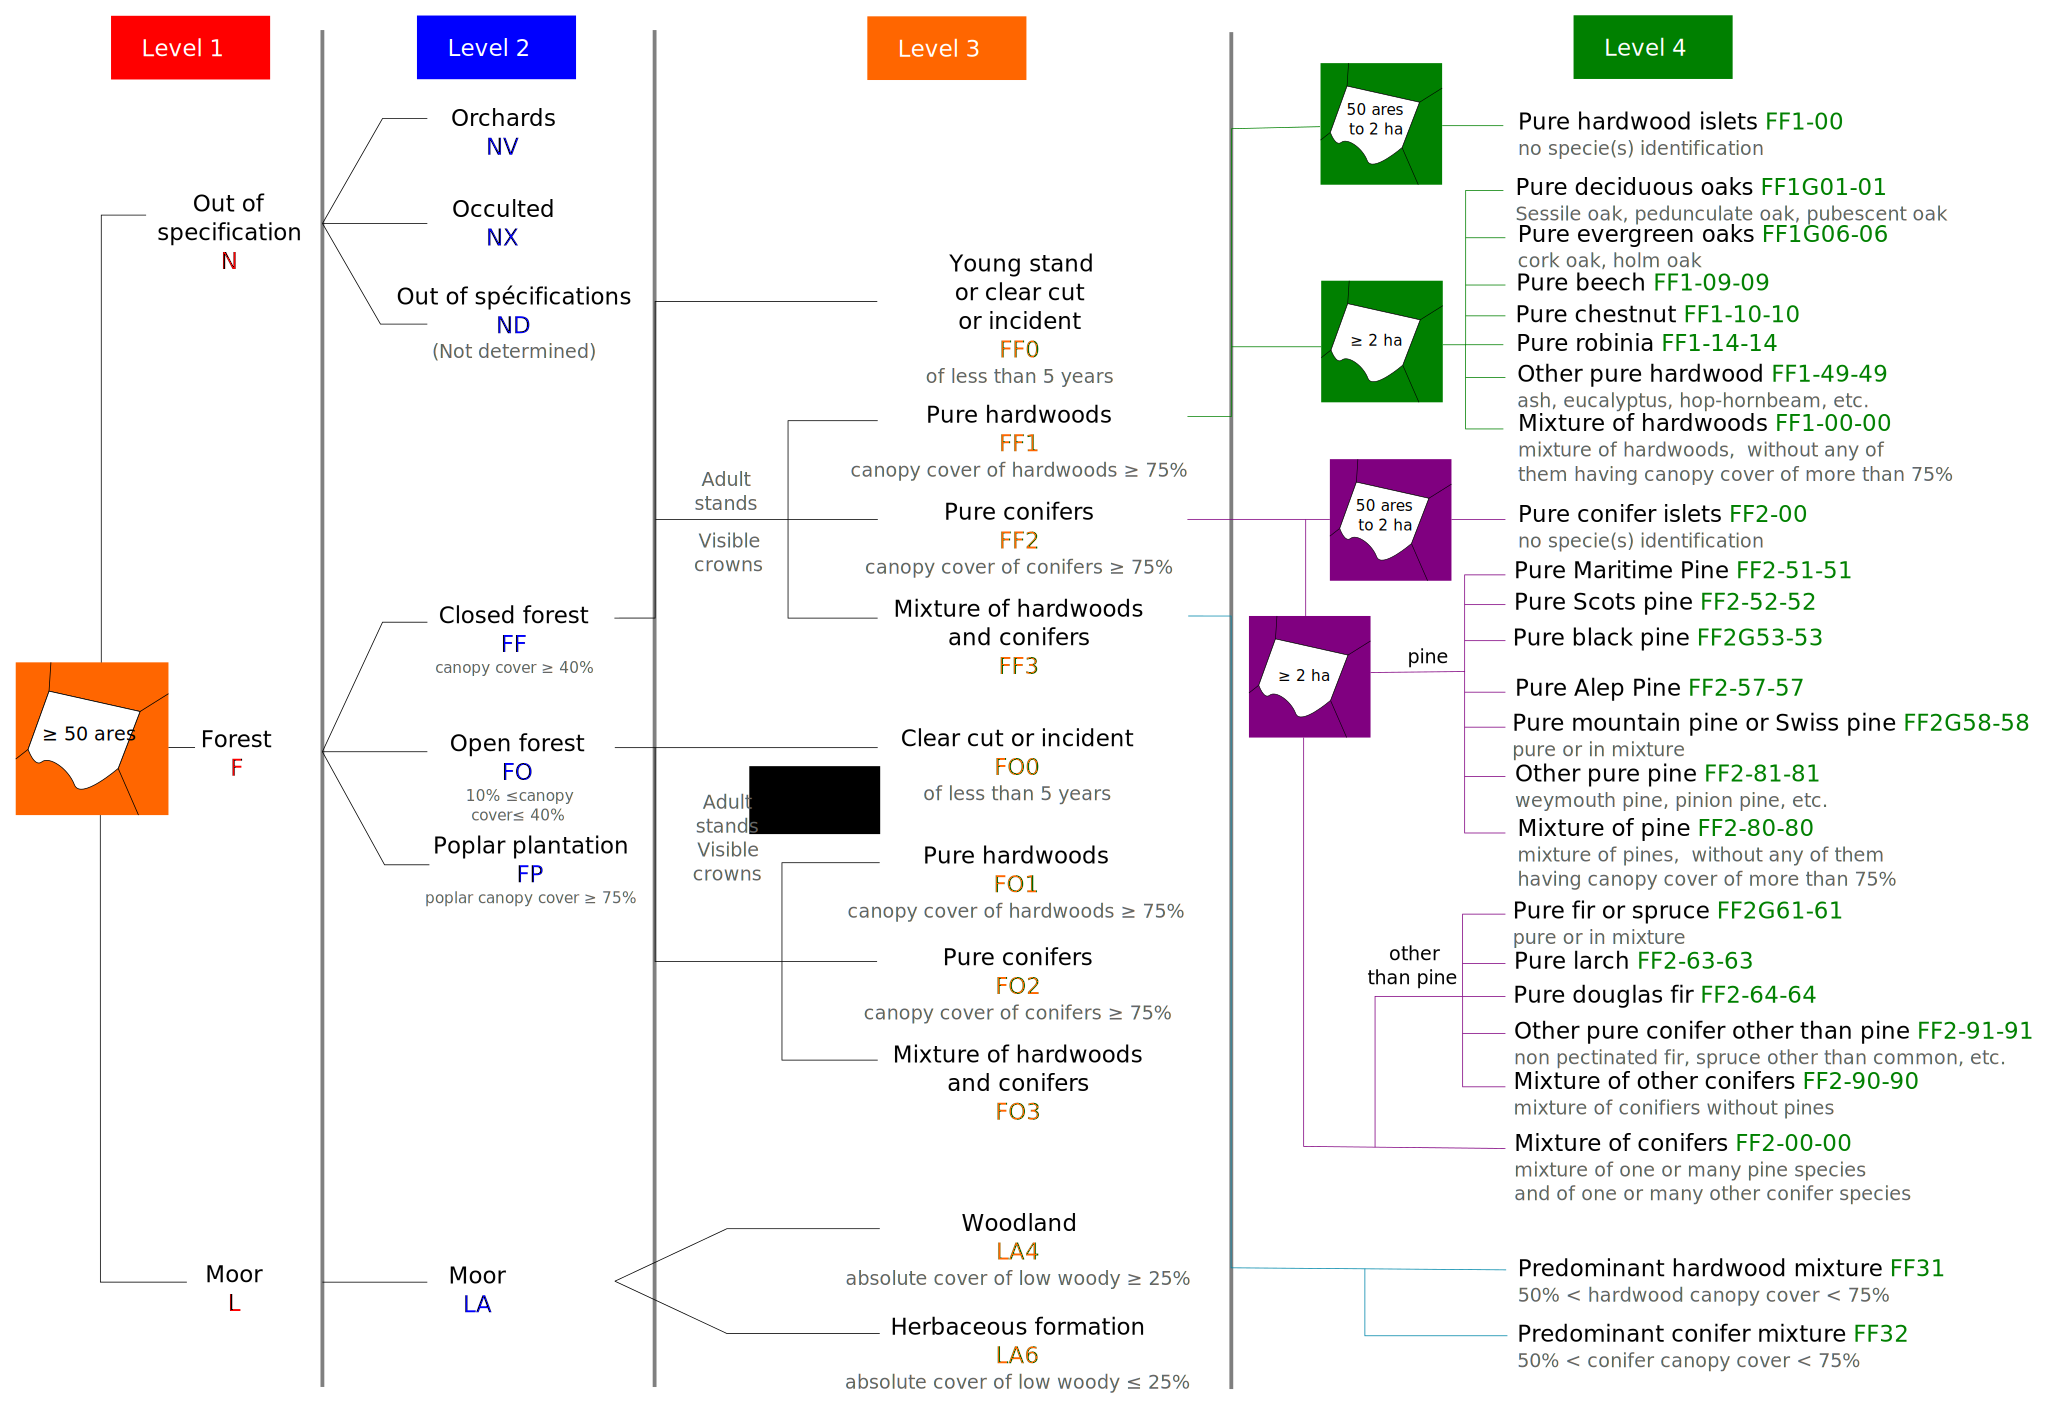
\includegraphics[width=\textwidth]{Figures/v2_organigram}
\caption{Organizational chart of the version 2 of the forest LC database.}
\label{fig:organigram_BD}
\end{center}
\end{figure}


\section{Segmentation methods}
A naive method to retrieve forest stands is to segment the input data. Such segmentation algorithms do not take into account the species information. Two algorithms were employed in order to obtain relevant stands only through the segmentation of the data.
The first segmentation algorithm is the one proposed in \cite{guigues2006scale}. It is a hierarchical segmentation algorithm that allows to control the level of segmentation through a unique scale parameter $\mu$.

The second segmentation algorithm (called here PFF) employed is presented in \cite{felzenszwalb2004efficient}. It is a method for image segmentation based on pairwise region comparison considering the minimum weight edge between two regions in measuring the difference between them. 3 simples parameters need to be tuned in order to obtain relevant segmentation. $\sigma$ is the standard deviation of the gaussian filter employed to smooth the image as a pre-processing (the authors recommend $\sigma=0.8$). $k$ is a second parameter that set a scale of observation (a larger $k$ will lead to larger segments). Finally, the parameter $m$ permits to define the minimum size of a segment.

Such segmentation could allow to retrieve the stands borders easily. Furthermore, one the segmentation is performed, one can add semantic information using classification results.

These experiments have been performed only on one area presented in Figure~\ref{fig:data_direct_seg}. It is a 1$\:$km$^{2}$ area, the spatial resolution of the VHR optical image is 0.5$\:$m, and the nDSM has been rasterized at the same resolution. From these data one can see that a stand is composed of zones that are not homogeneous in term of reflectance and/or height. Furthermore, one can also note that the variability between two stands in terms of reflectance and/or height might not be important.

\begin{figure}[htbp]
\begin{center}
\begingroup
\captionsetup[subfigure]{width=0.16\textwidth}
\subfloat[VHR IRC optical image.]{
\includegraphics[width=0.3\textwidth]{Figures/C3/S2/IRC}
\label{subfig:data_direct_sega}
}
\subfloat[nDSM.]{
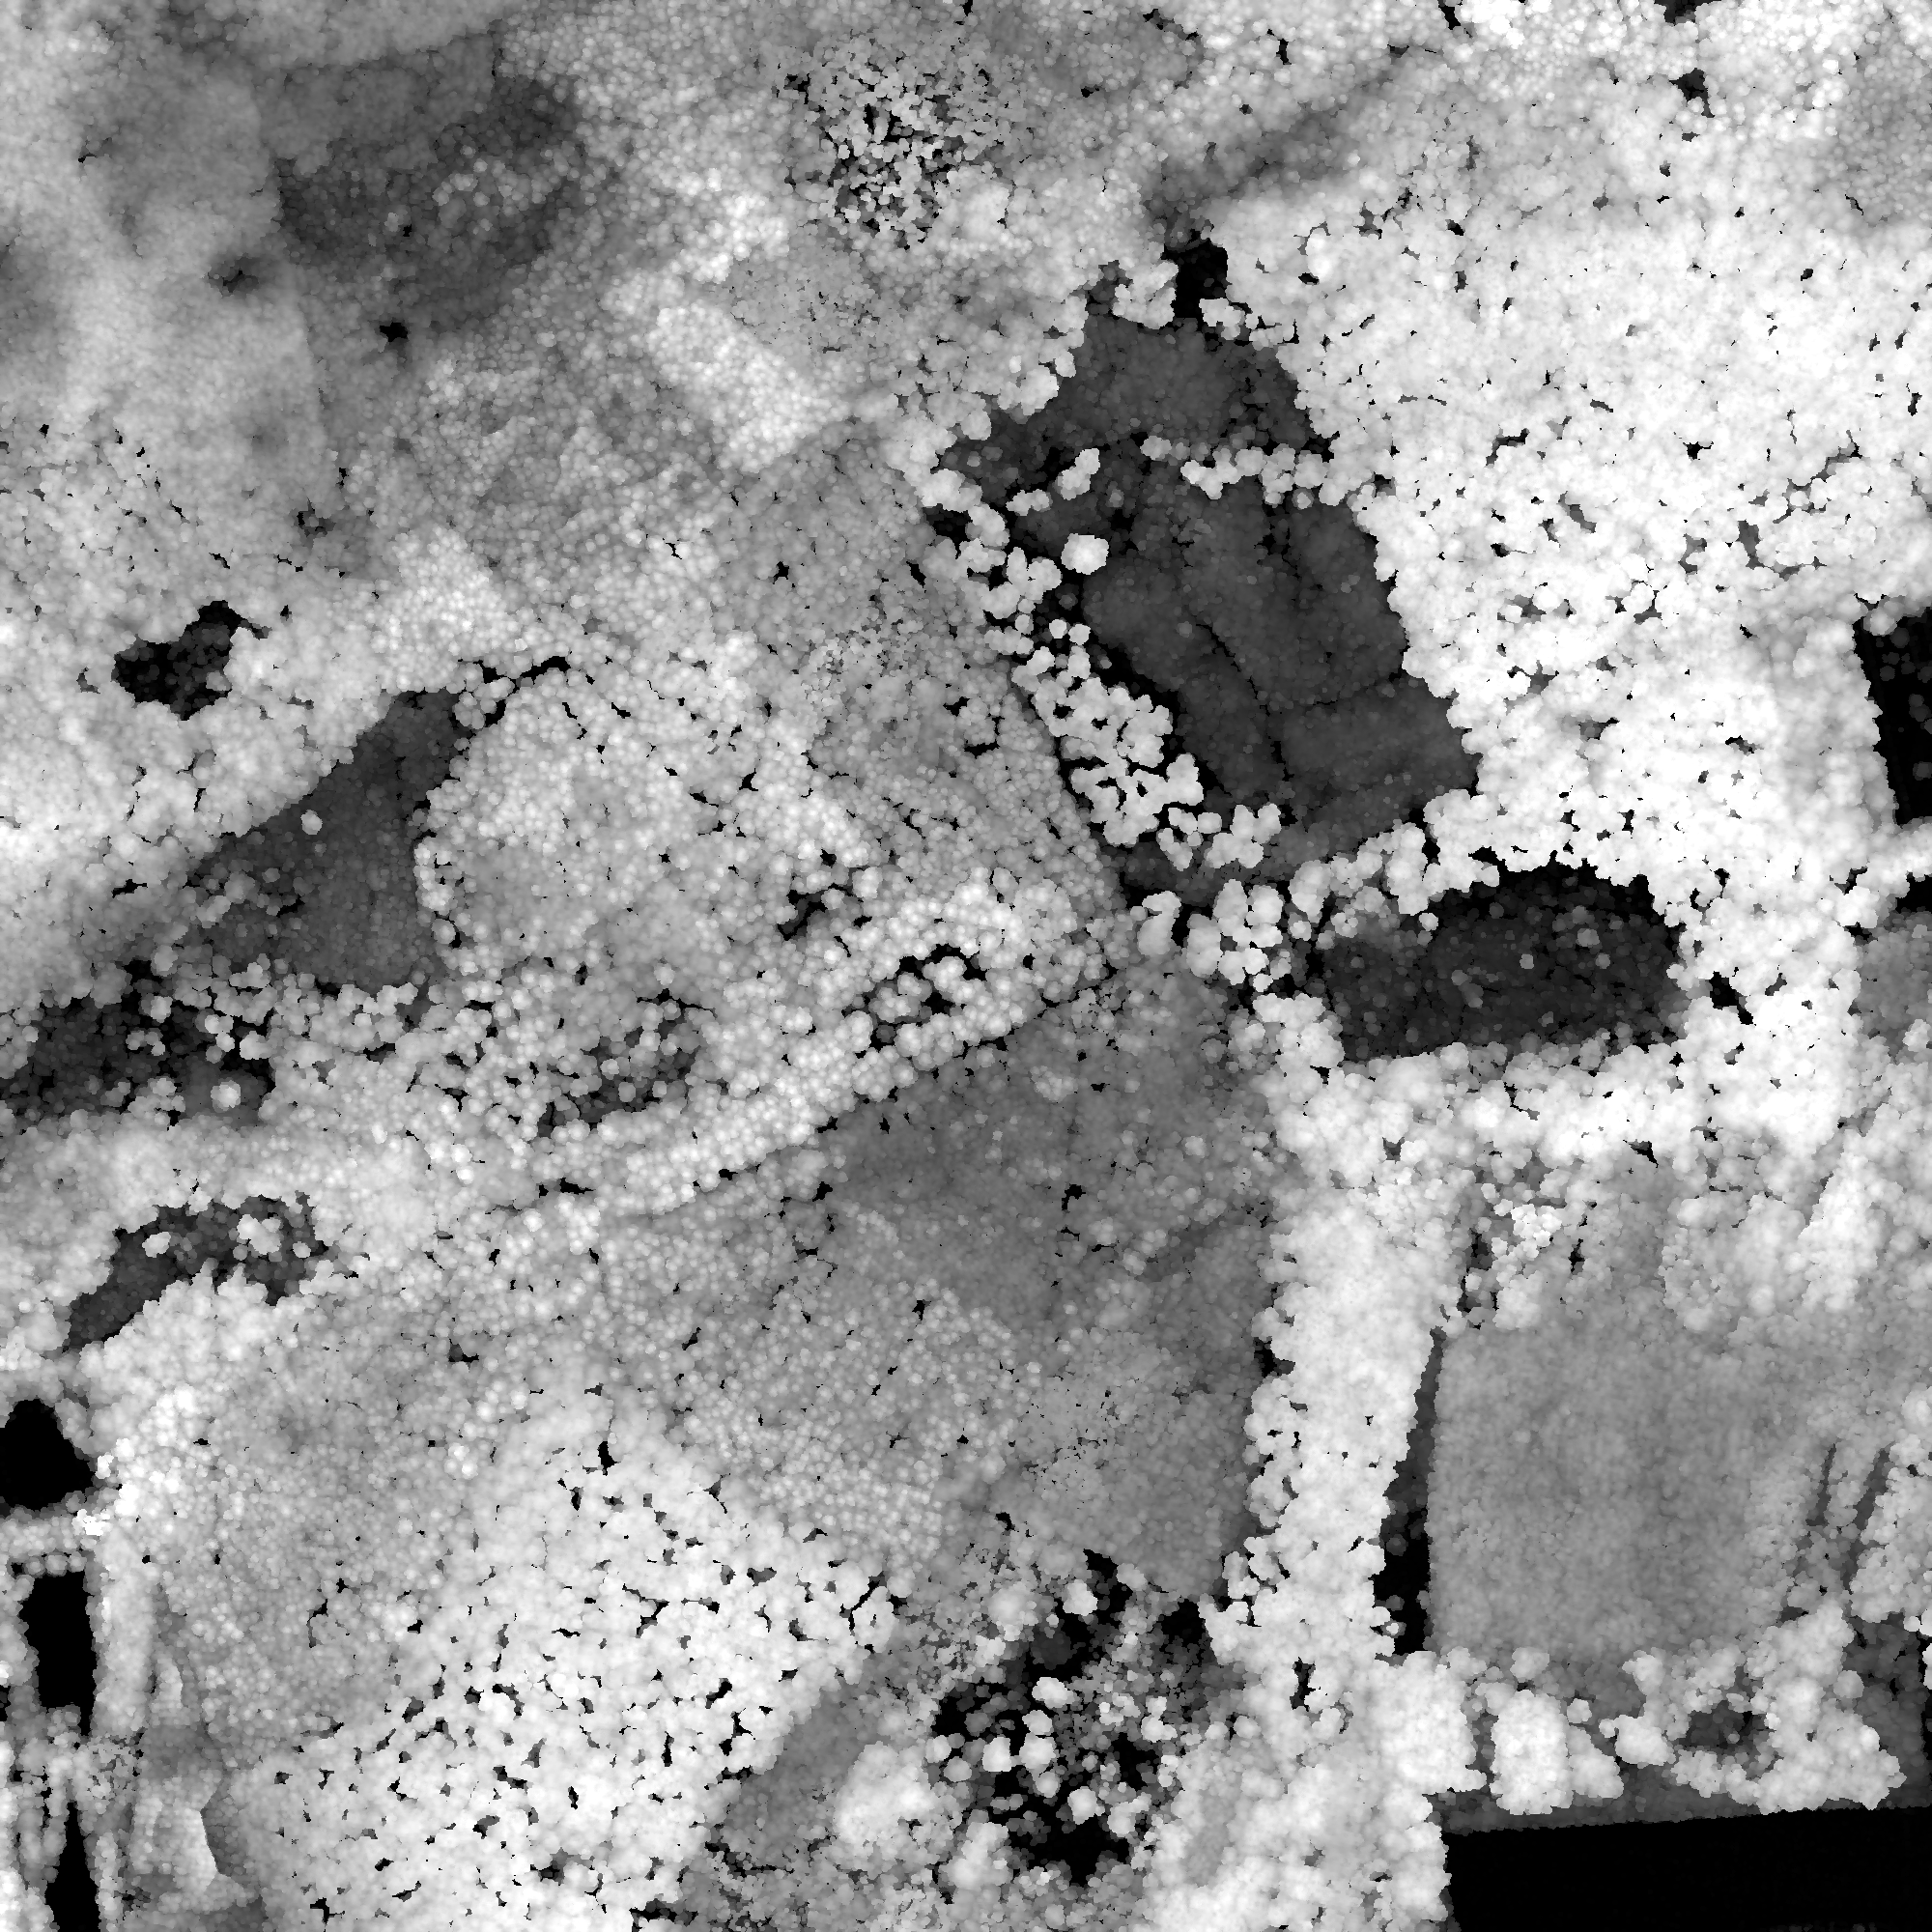
\includegraphics[width=0.3\textwidth]{Figures/C3/S2/nDSM}
\label{subfig:data_direct_segb}
}
\subfloat[Forest LC database.]{
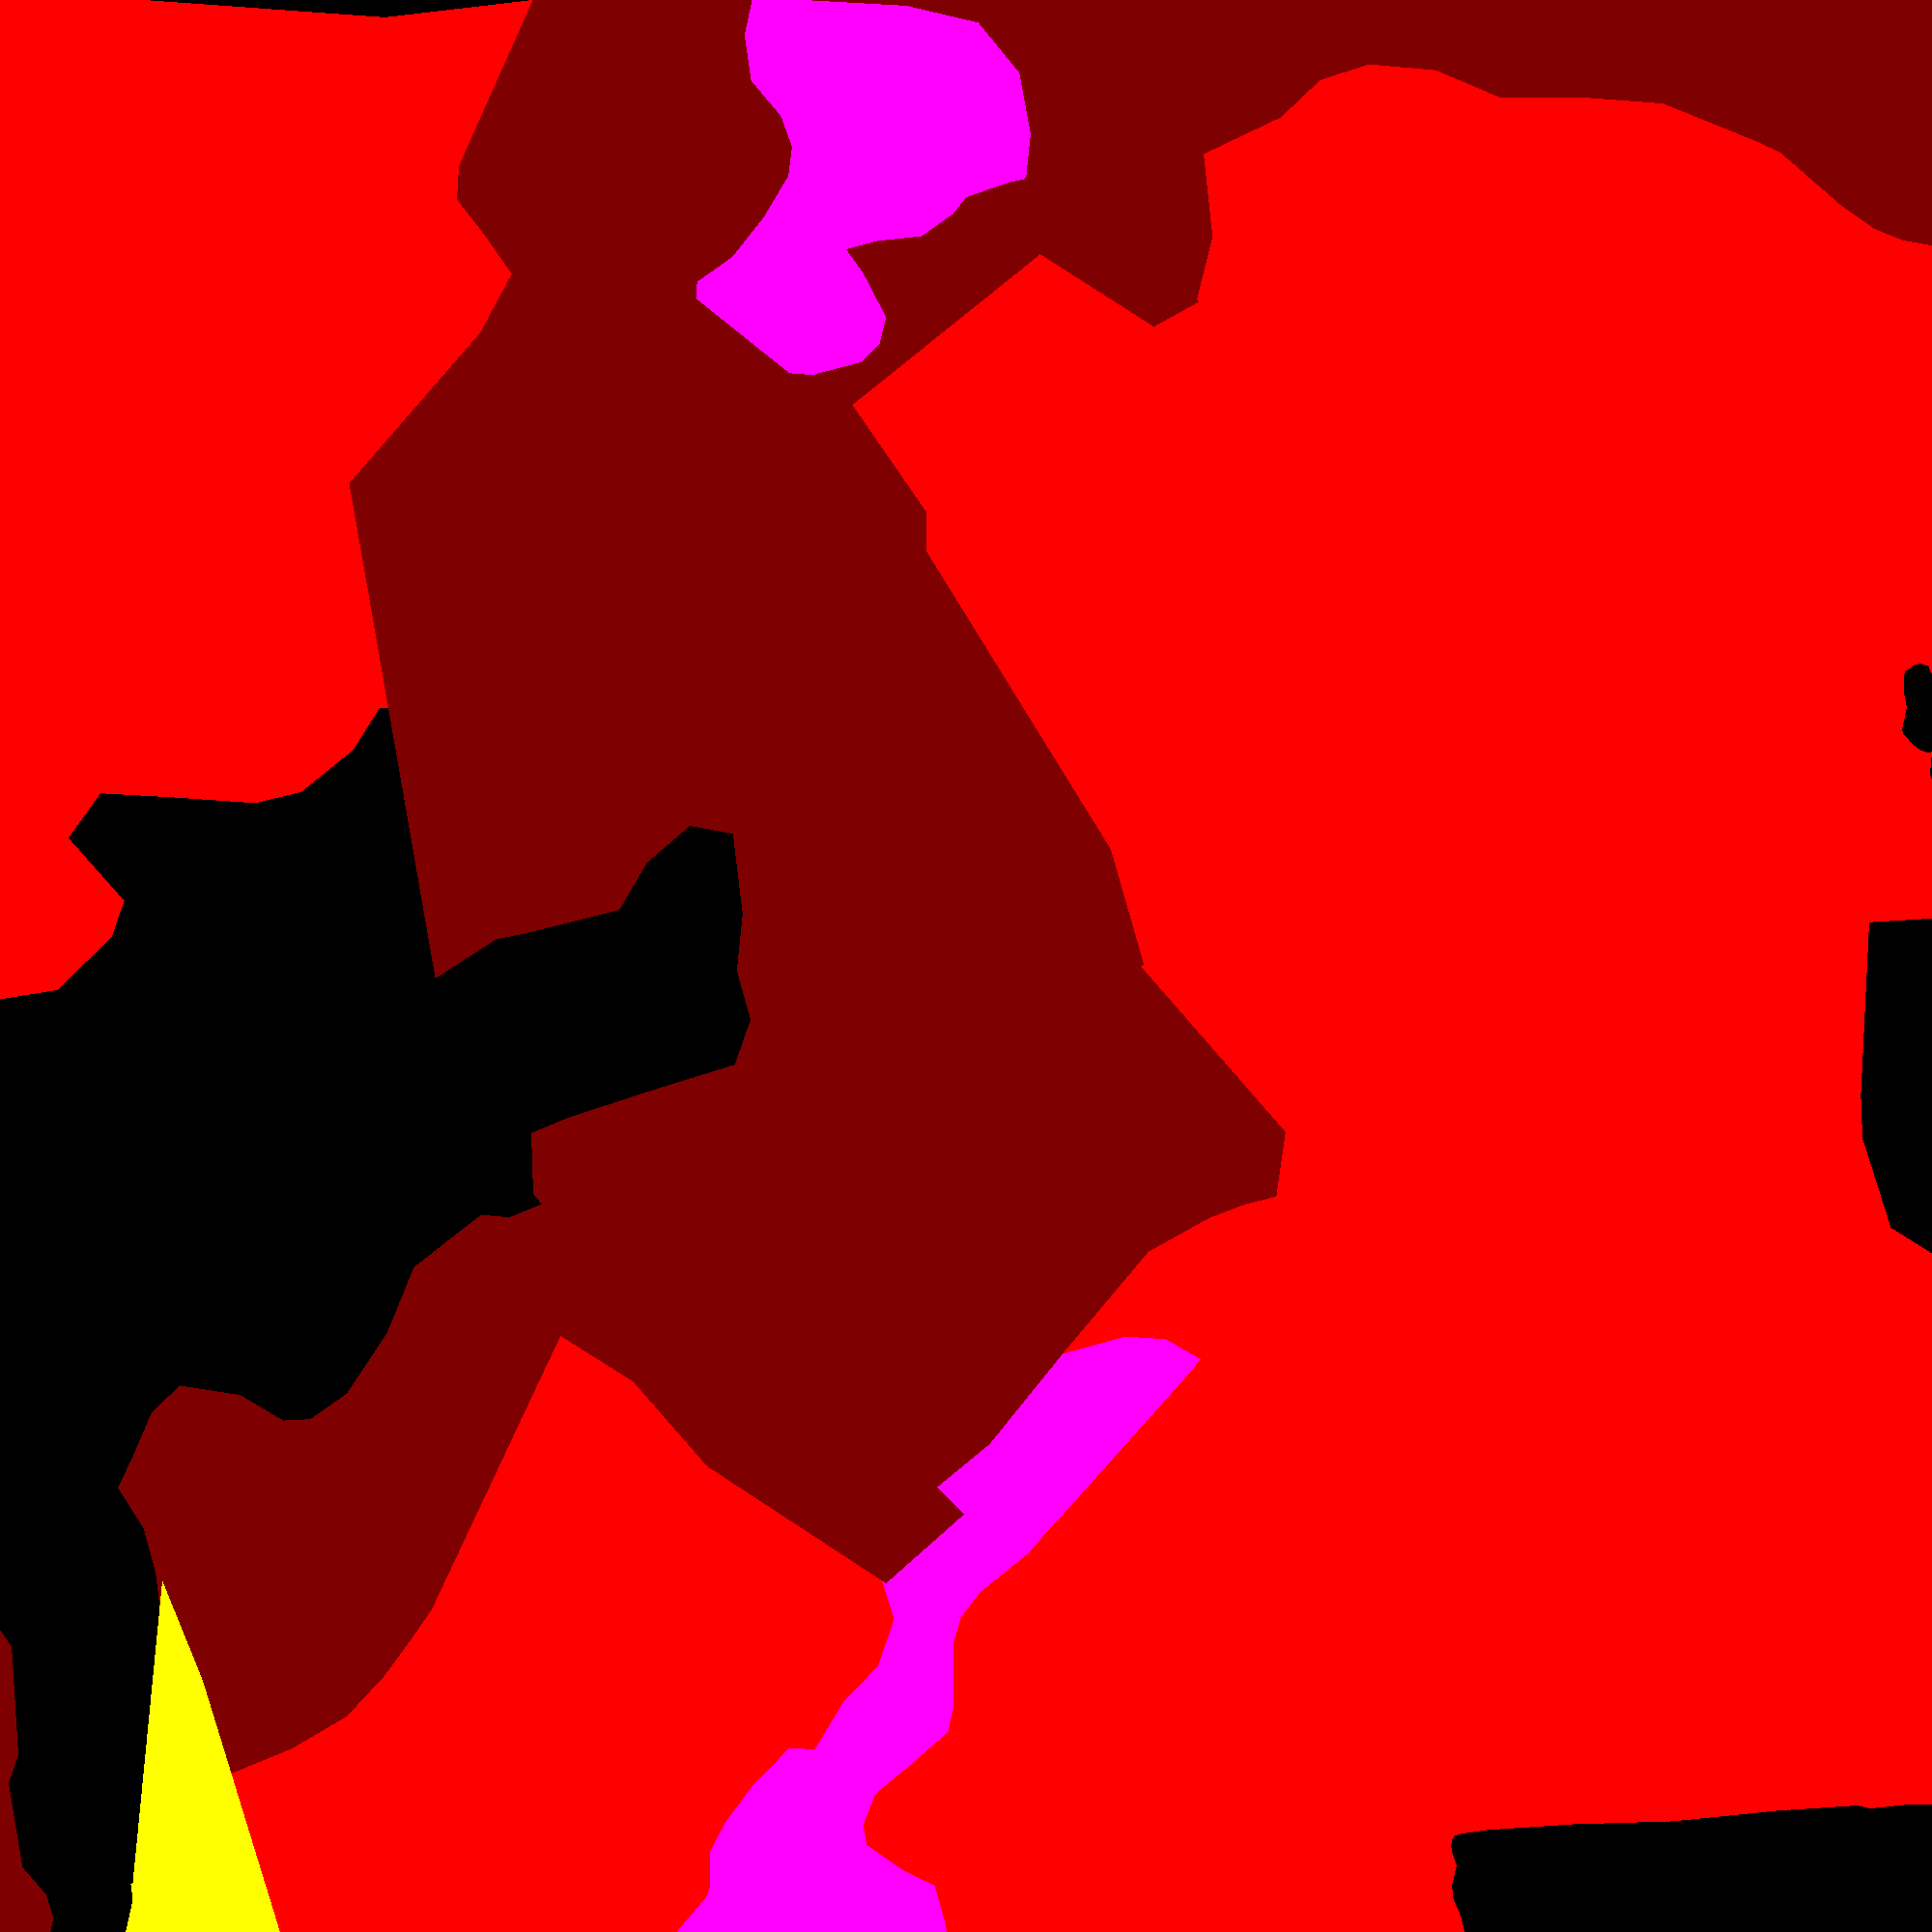
\includegraphics[width=0.3\textwidth]{Figures/C3/S2/BD}
\label{subfig:data_direct_segc}
}
\endgroup
\caption{VHR IRC optical image, rasterized nDSM and forest LC of the proposed area for the direct segmentation tests.}
\label{fig:data_direct_seg}
\end{center}
\end{figure}

\subsection{Retrieve stands borders}
\label{sec:C3_S2_ss1}
Two strategies are employed to apply the segmentation in order to retrieve the forest stands borders from the forest LC database:
\begin{itemize}
\item The segmentation is applied to the VHR optical images, thus the resulting segment will correspond to "stands" that are homogeneous in terms of spectral reflectance. Since the optical images are employed by photo-interpreters in order to derive the forest LC, such segmentation should produce results similar to the forest LC.
\item The segmentation is also applied to the rasterized normalized digital surface model (nDSM) (canopy height without ground relief). Such segmentation would produce "stands" that are homogeneous in term of height.
\end{itemize}

The results of the segmentation of the VHR optical image using the two segmentation algorithm is presented in Figure~\ref{fig:seg_im}. In both cases, most of the borders found are not consistent with the forest LC database. Visually, the hierarchical segmentation seems to be more relevant than the PFF segmentation. However, the hierarchical segmentation produces small segments due to high variation of illumination in the image, while the PFF segments are all relatively large. 

\begin{figure}[htbp]
\begin{center}
\begingroup
\captionsetup[subfigure]{width=0.4\textwidth}
\subfloat[Hierarchical segmentation with $\mu=15$.]{
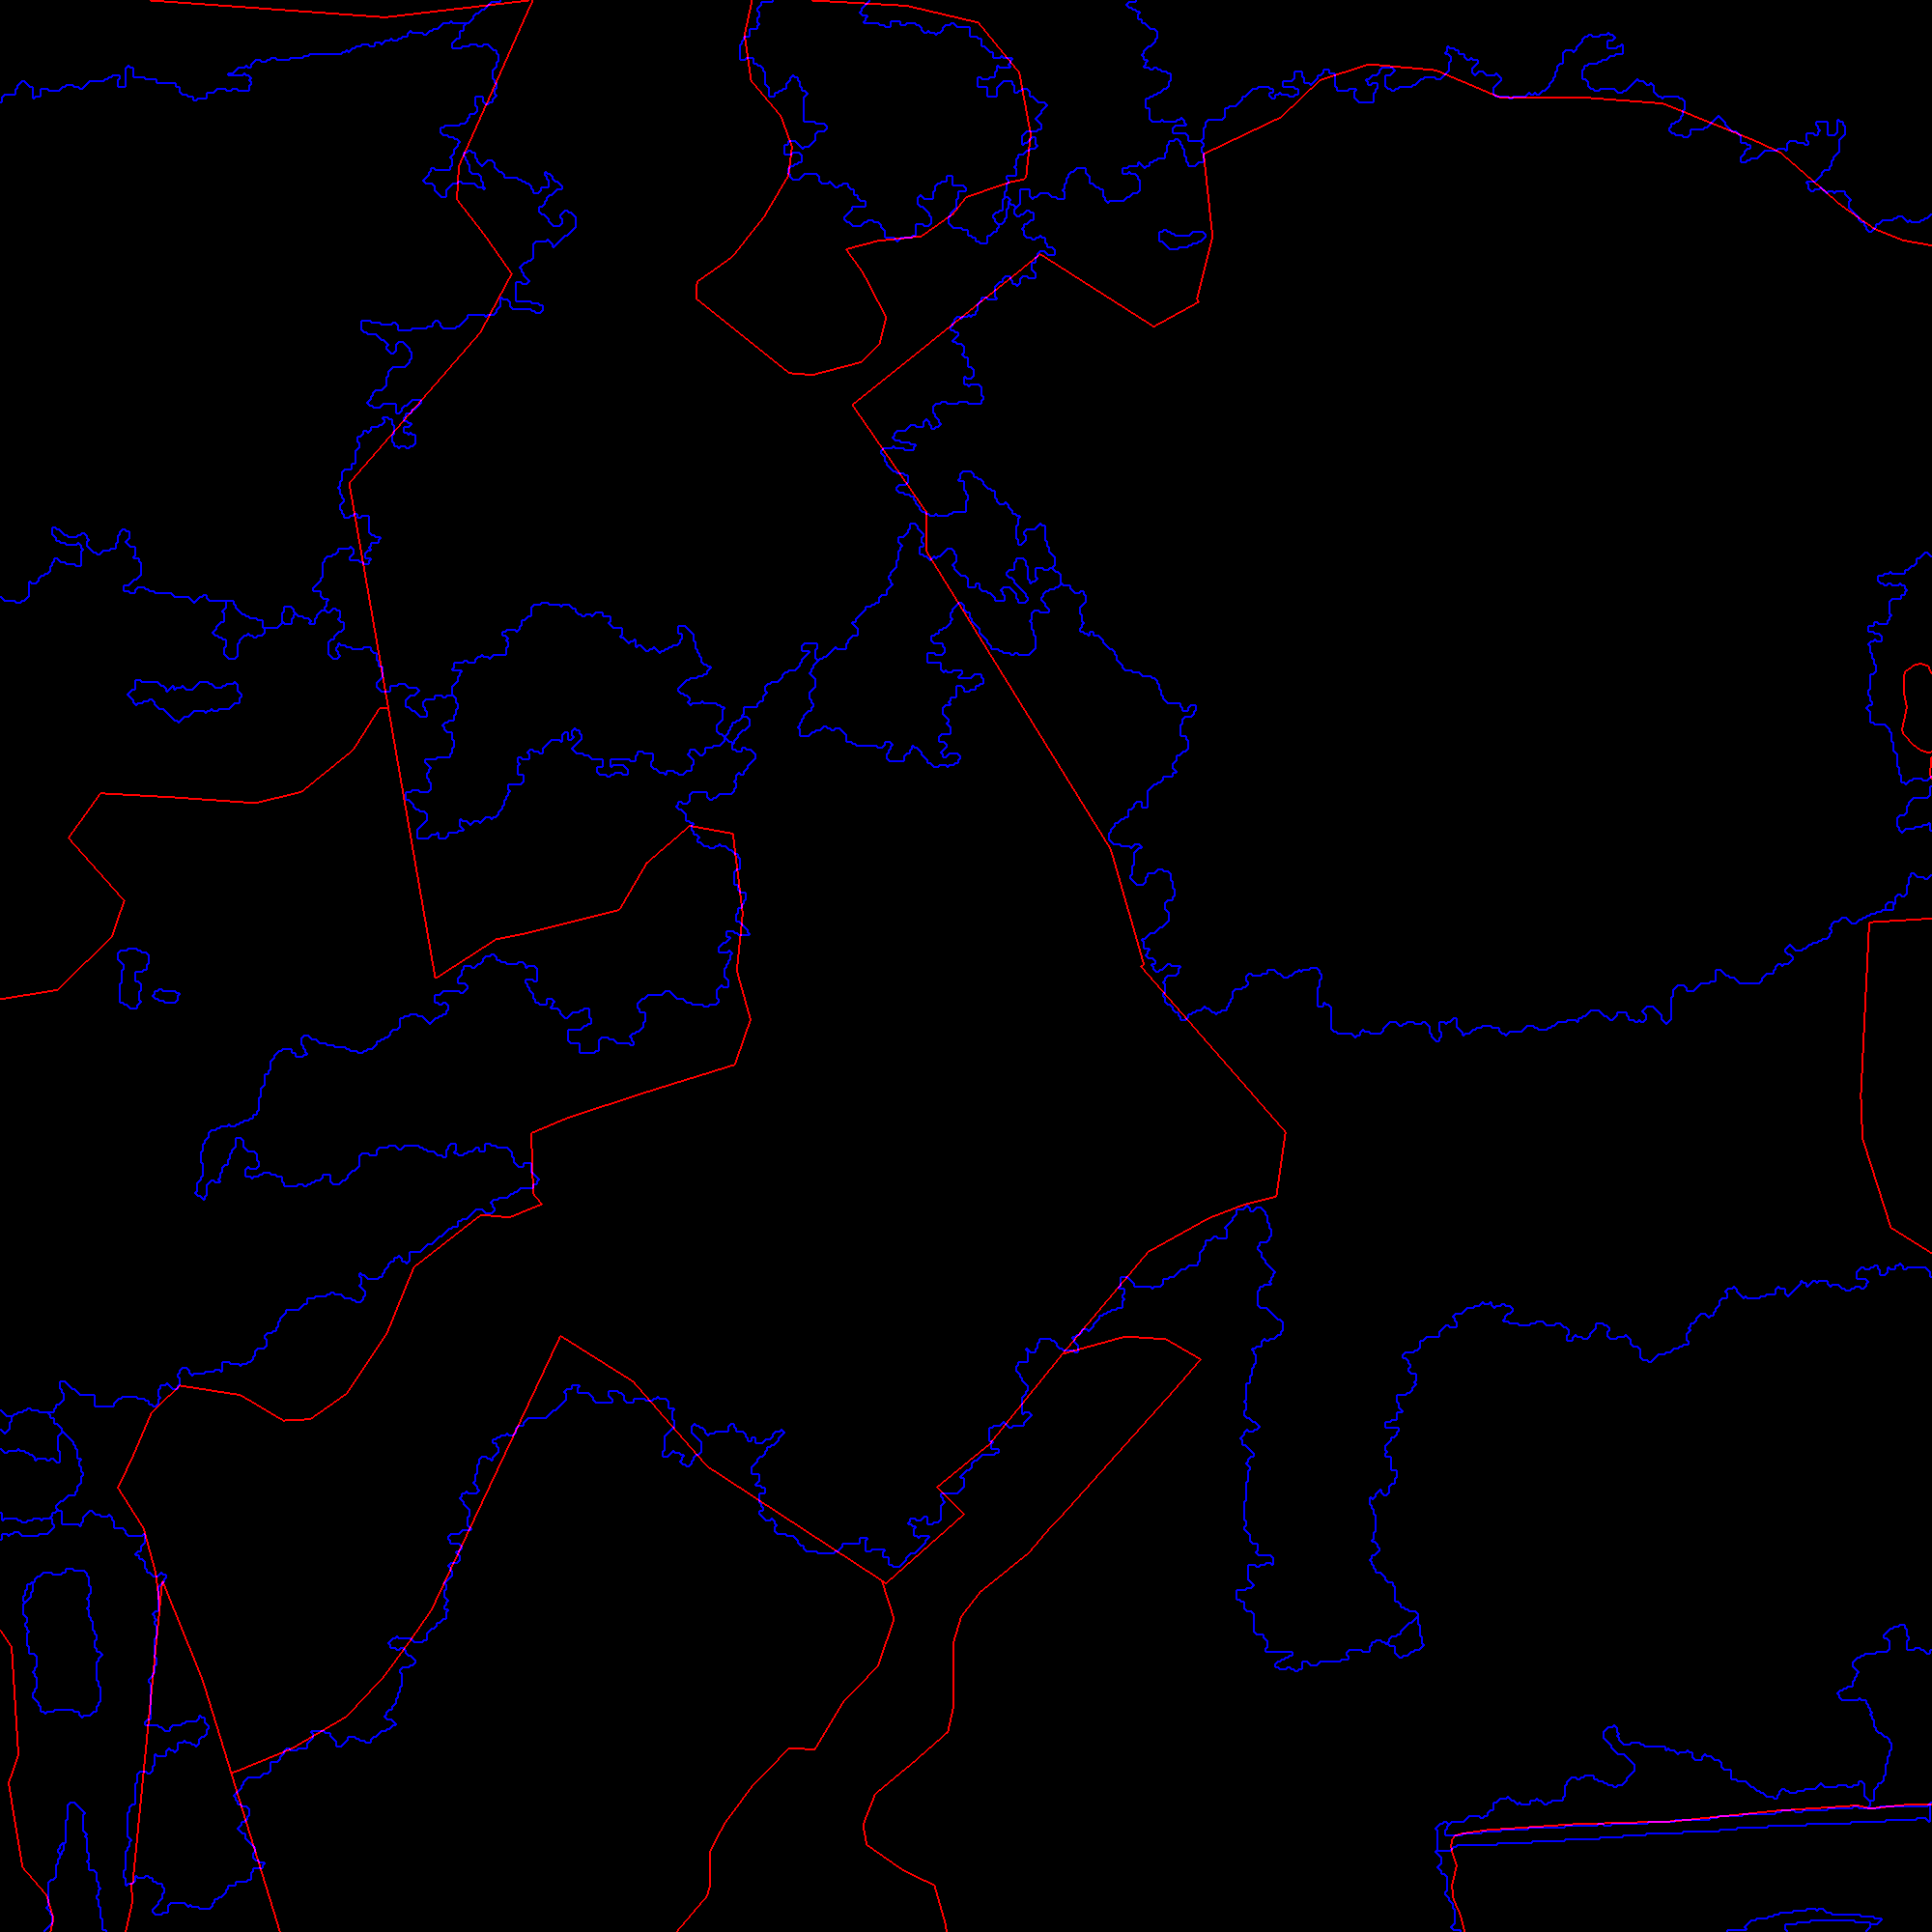
\includegraphics[width=0.45\textwidth]{Figures/C3/S2/border_hierar}
\label{subfig:seg_ima}
}
\hspace*{0.05\textwidth}
\subfloat[PFF segmentation with $\sigma=0.8$, $k=500$ and $m=40000$.]{
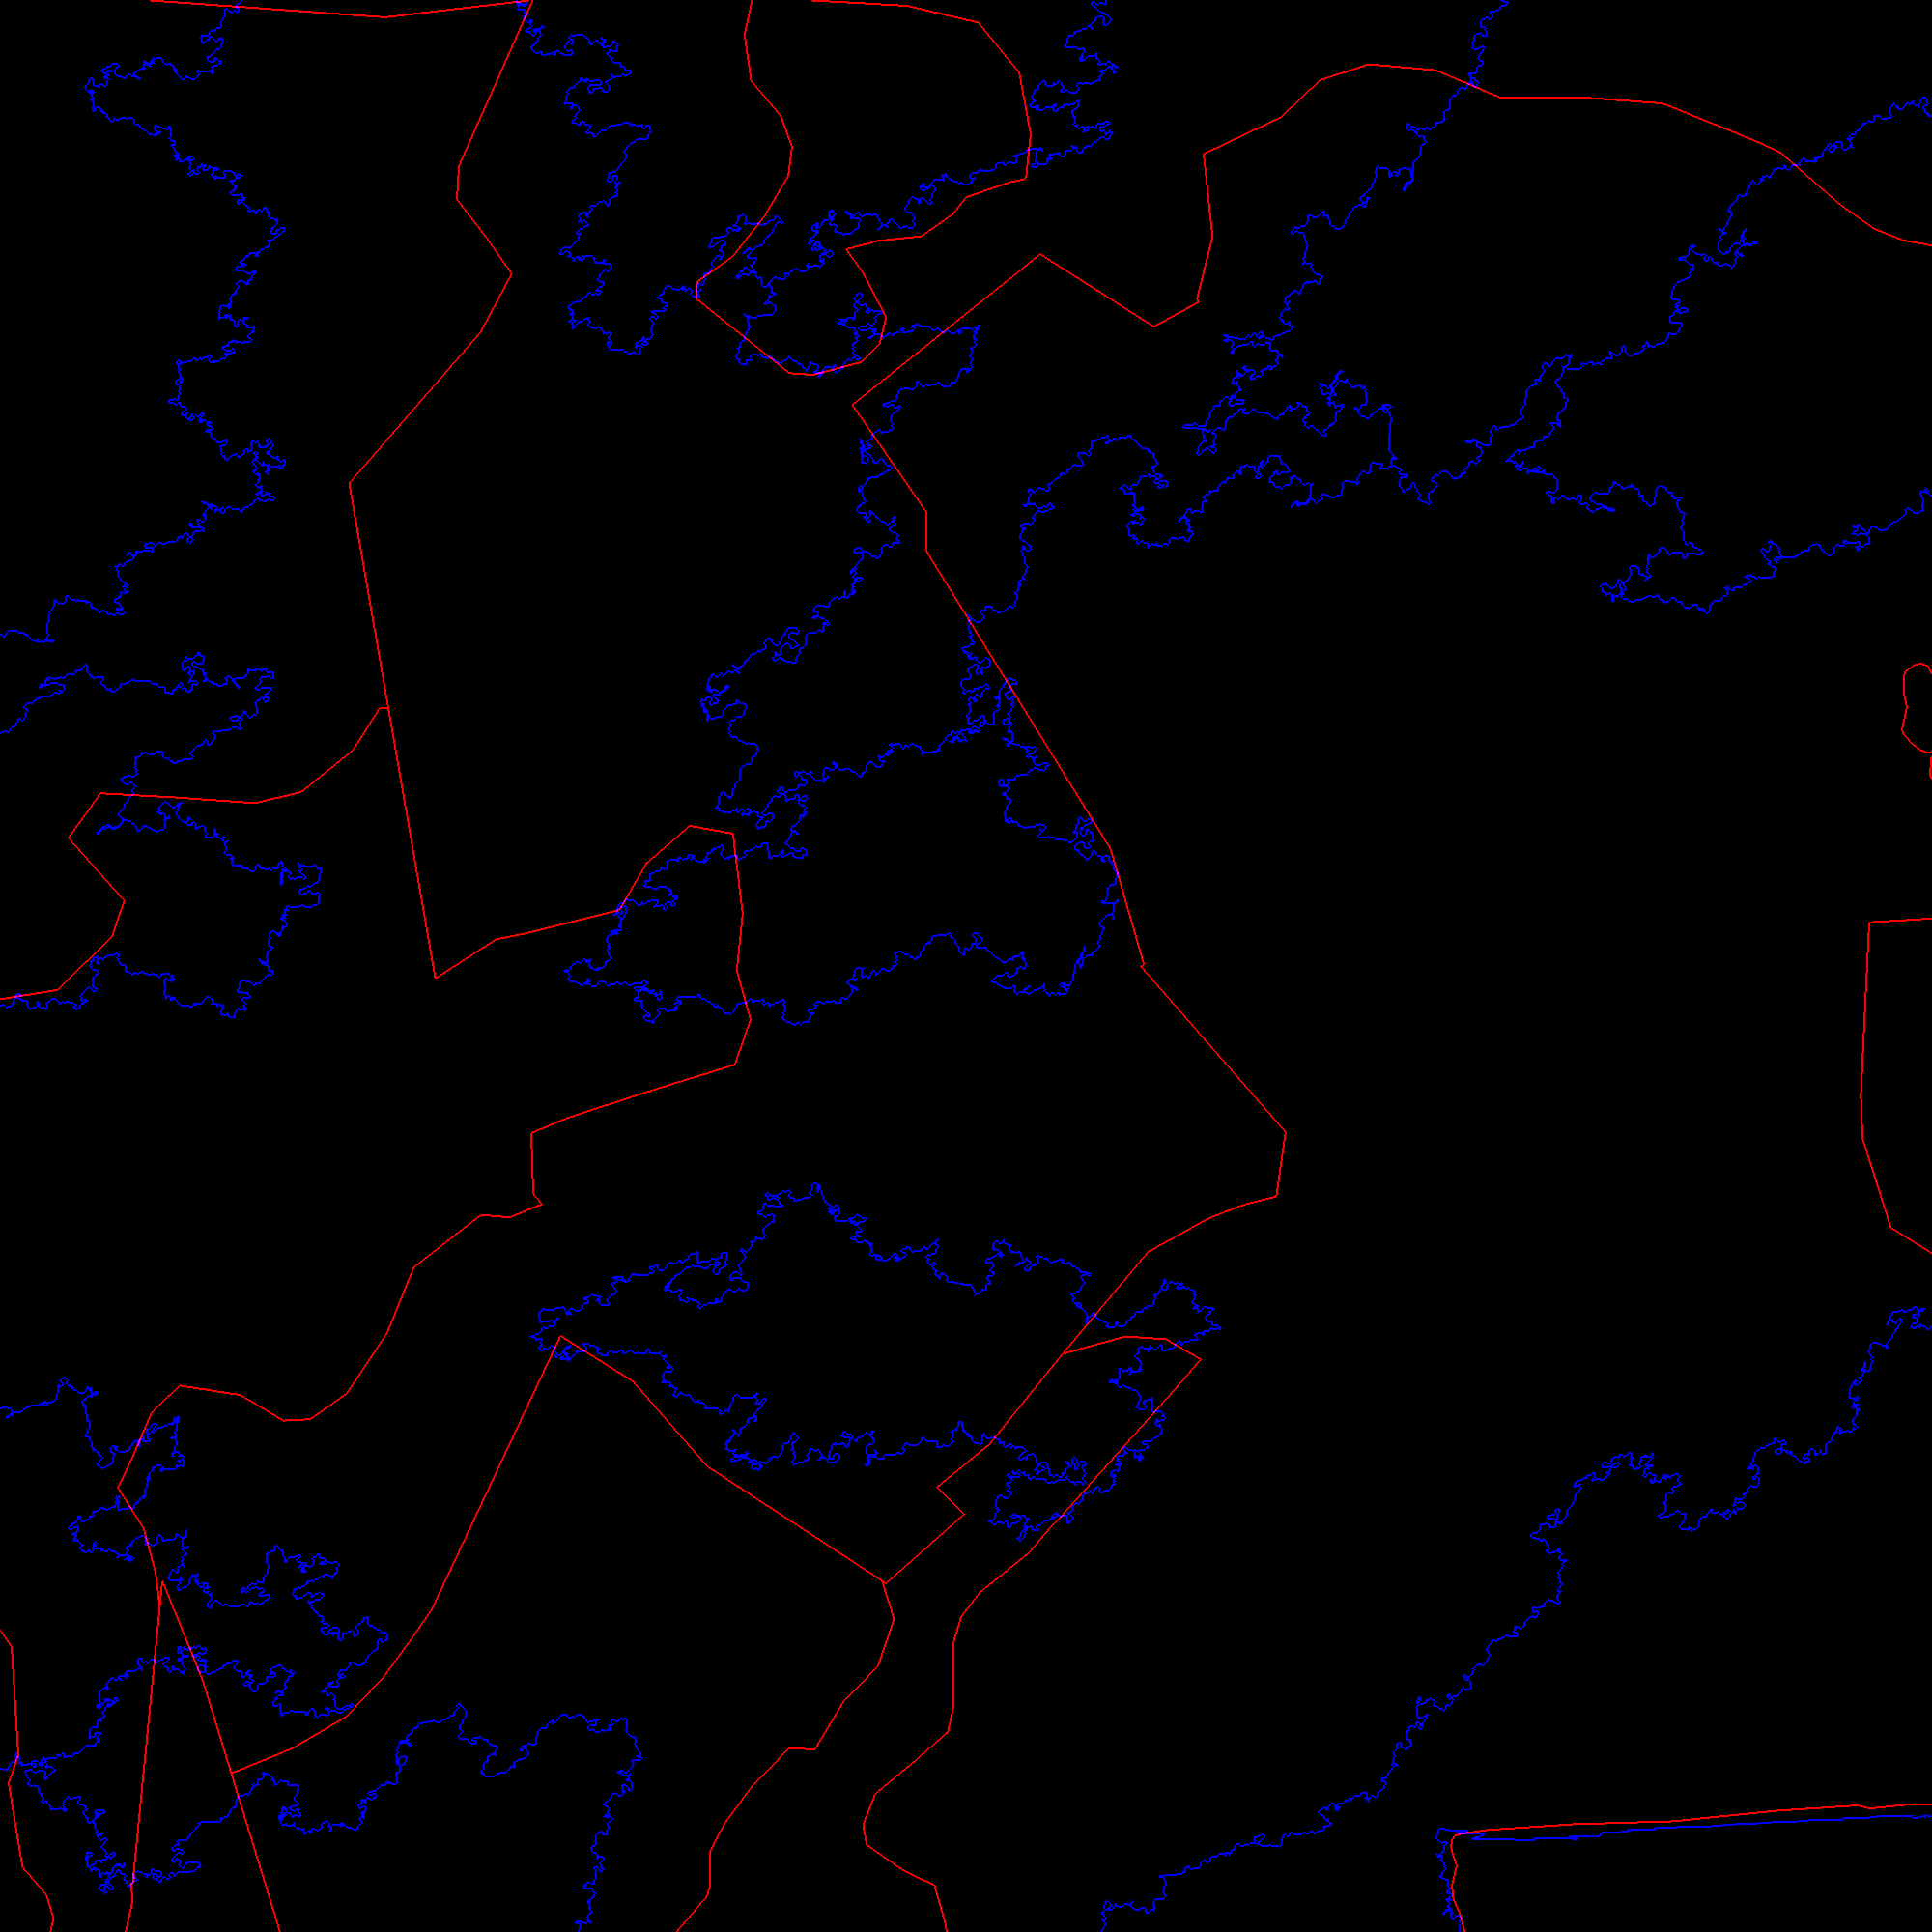
\includegraphics[width=0.45\textwidth]{Figures/C3/S2/border_PFF_IRC}
\label{subfig:seg_imb}
}
\endgroup
\caption{Result of the segmentation of the VHR optical image for the two segmentation algorithms. Blue lines correspond to the borders of the segments, red lines correspond to the borders of the forest LC.}
\label{fig:seg_im}
\end{center}
\end{figure}

The results of the segmentation of rasterized nDSM using the two segmentation algorithm is presented in Figure~\ref{fig:seg_nDSM}. Just like the segmentation of the VHR optical image, most of the borders found are not consistent with the forest LC database. Here, the PFF segmentation seems to perform better than the hierarchical segmentation visually.


\begin{figure}[htbp]
\begin{center}
\begingroup
\captionsetup[subfigure]{width=0.4\textwidth}
\subfloat[Hierarchical segmentation with $\mu=15$.]{
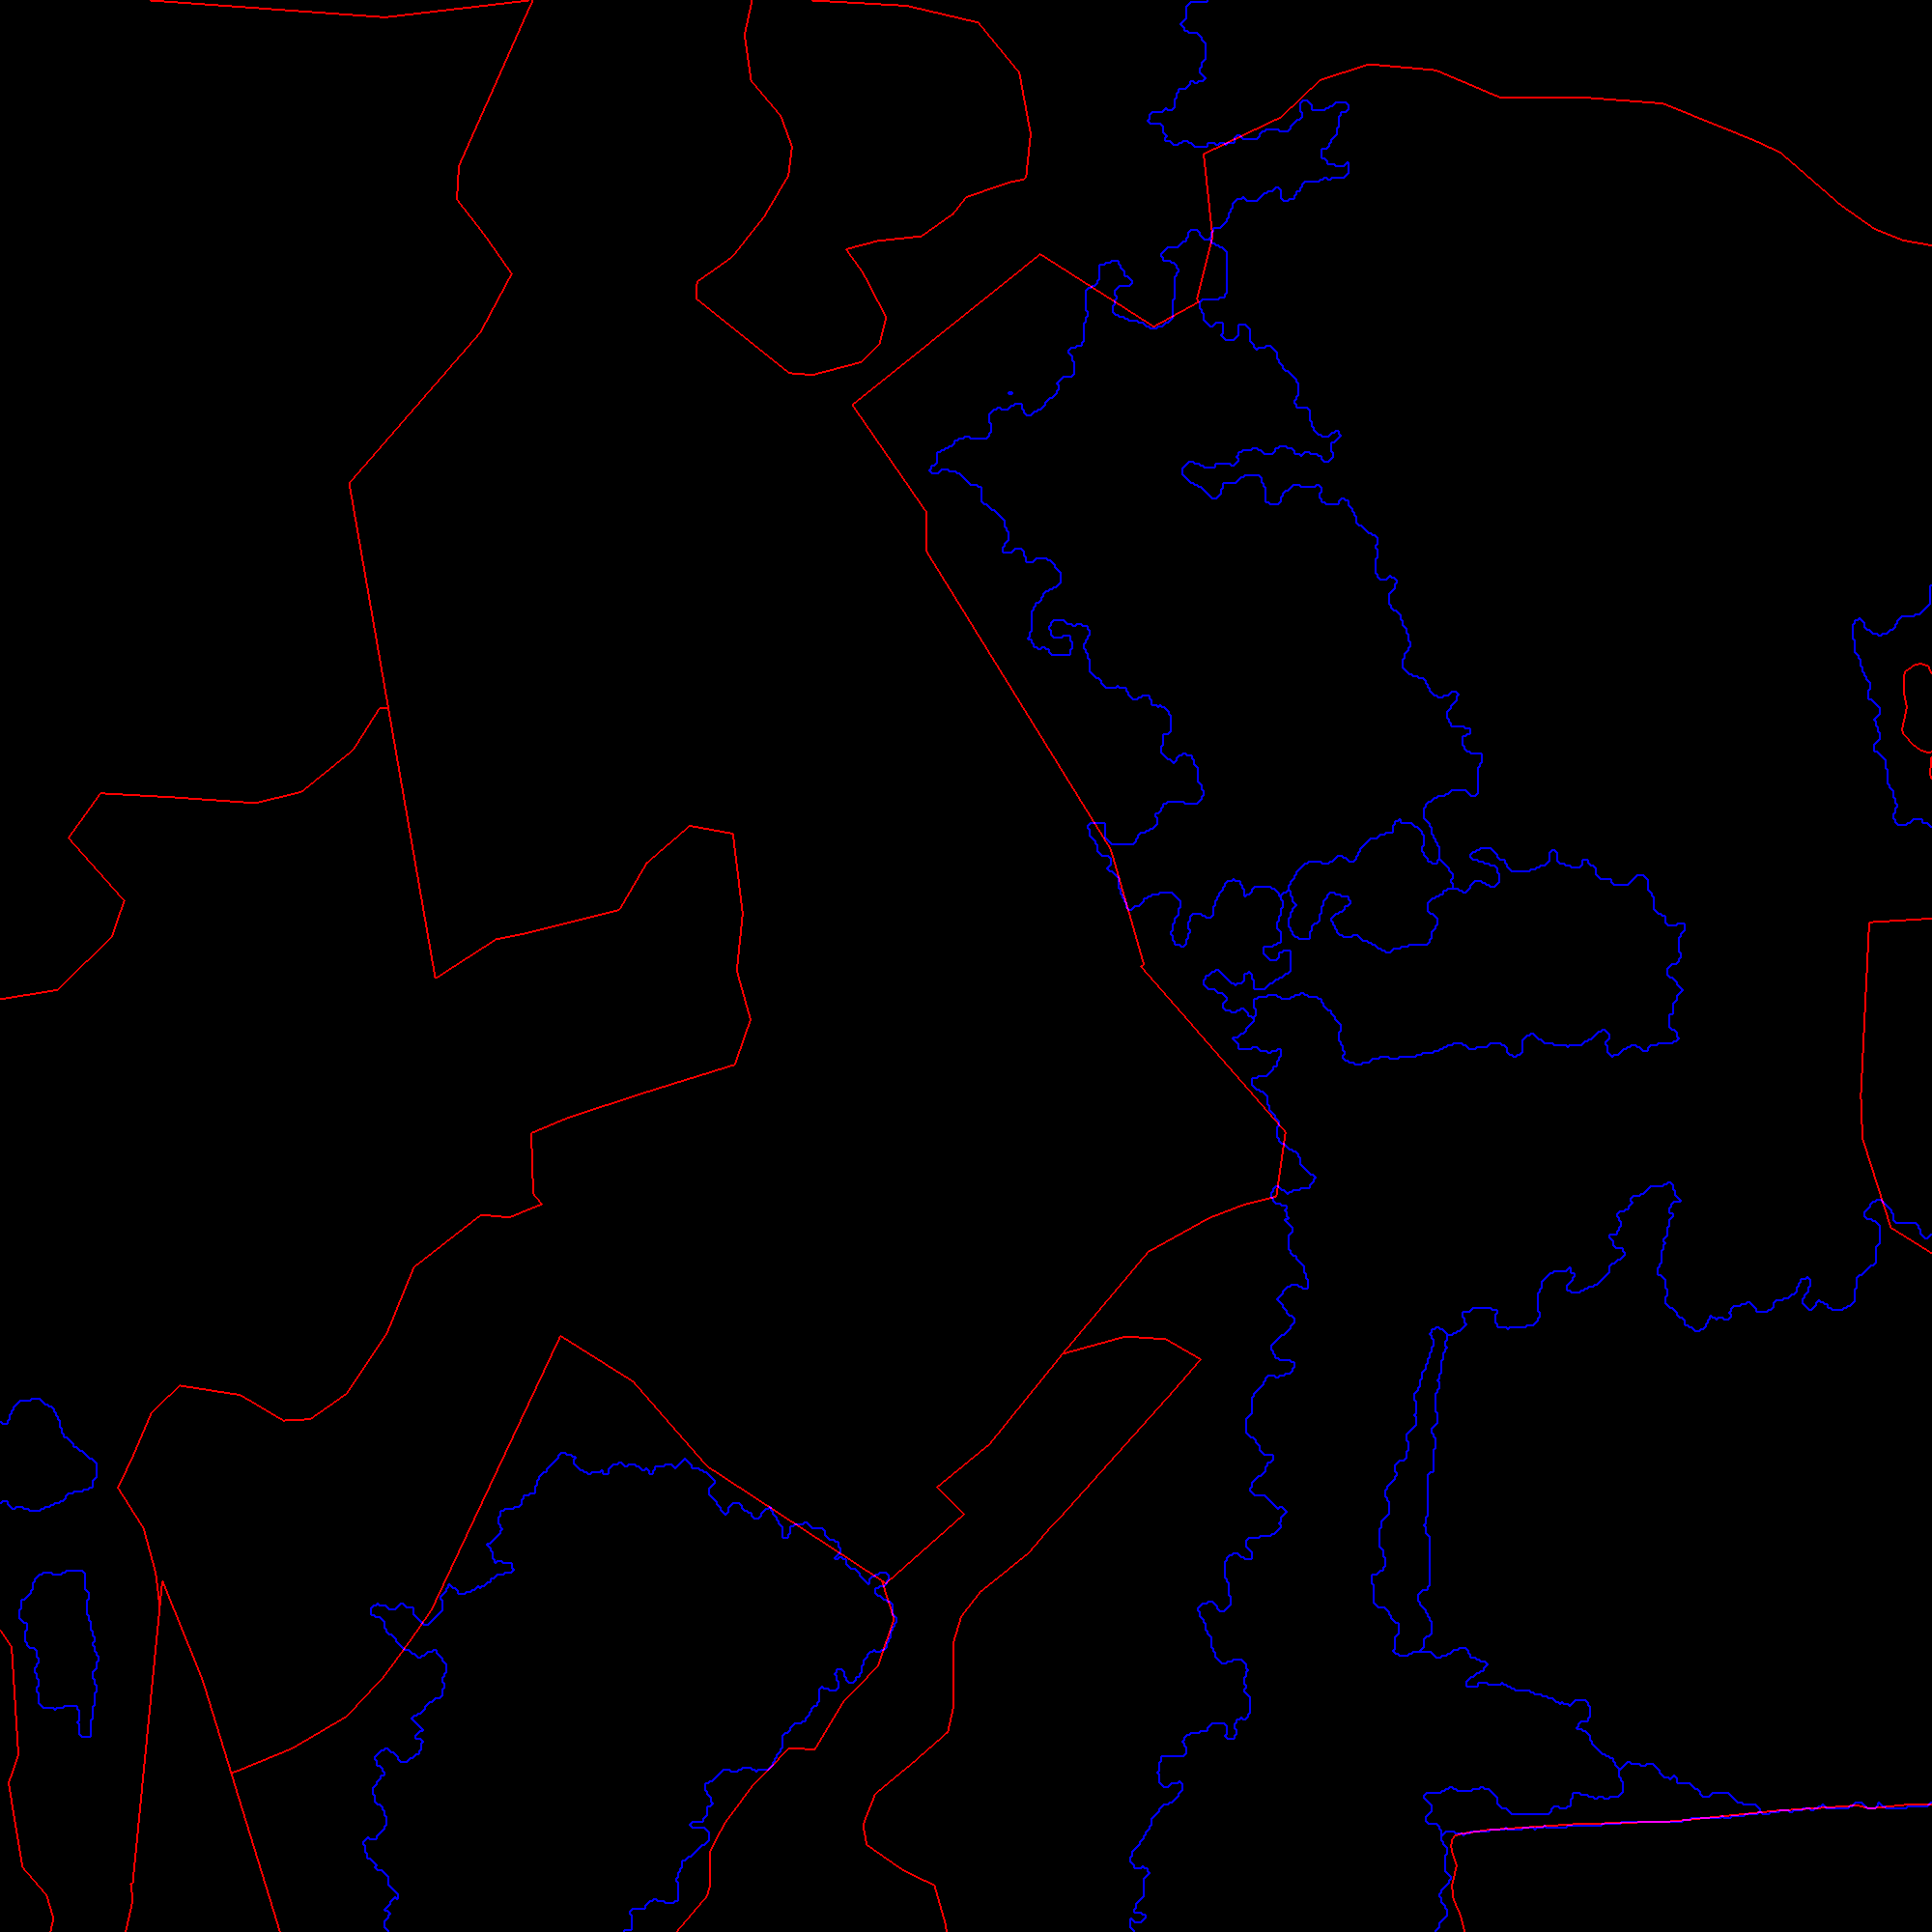
\includegraphics[width=0.45\textwidth]{Figures/C3/S2/border_hierar_z}
\label{subfig:seg_nDSMa}
}
\hspace*{0.05\textwidth}
\subfloat[PFF segmentation with $\sigma=0.8$, $k=500$ and $m=40000$.]{
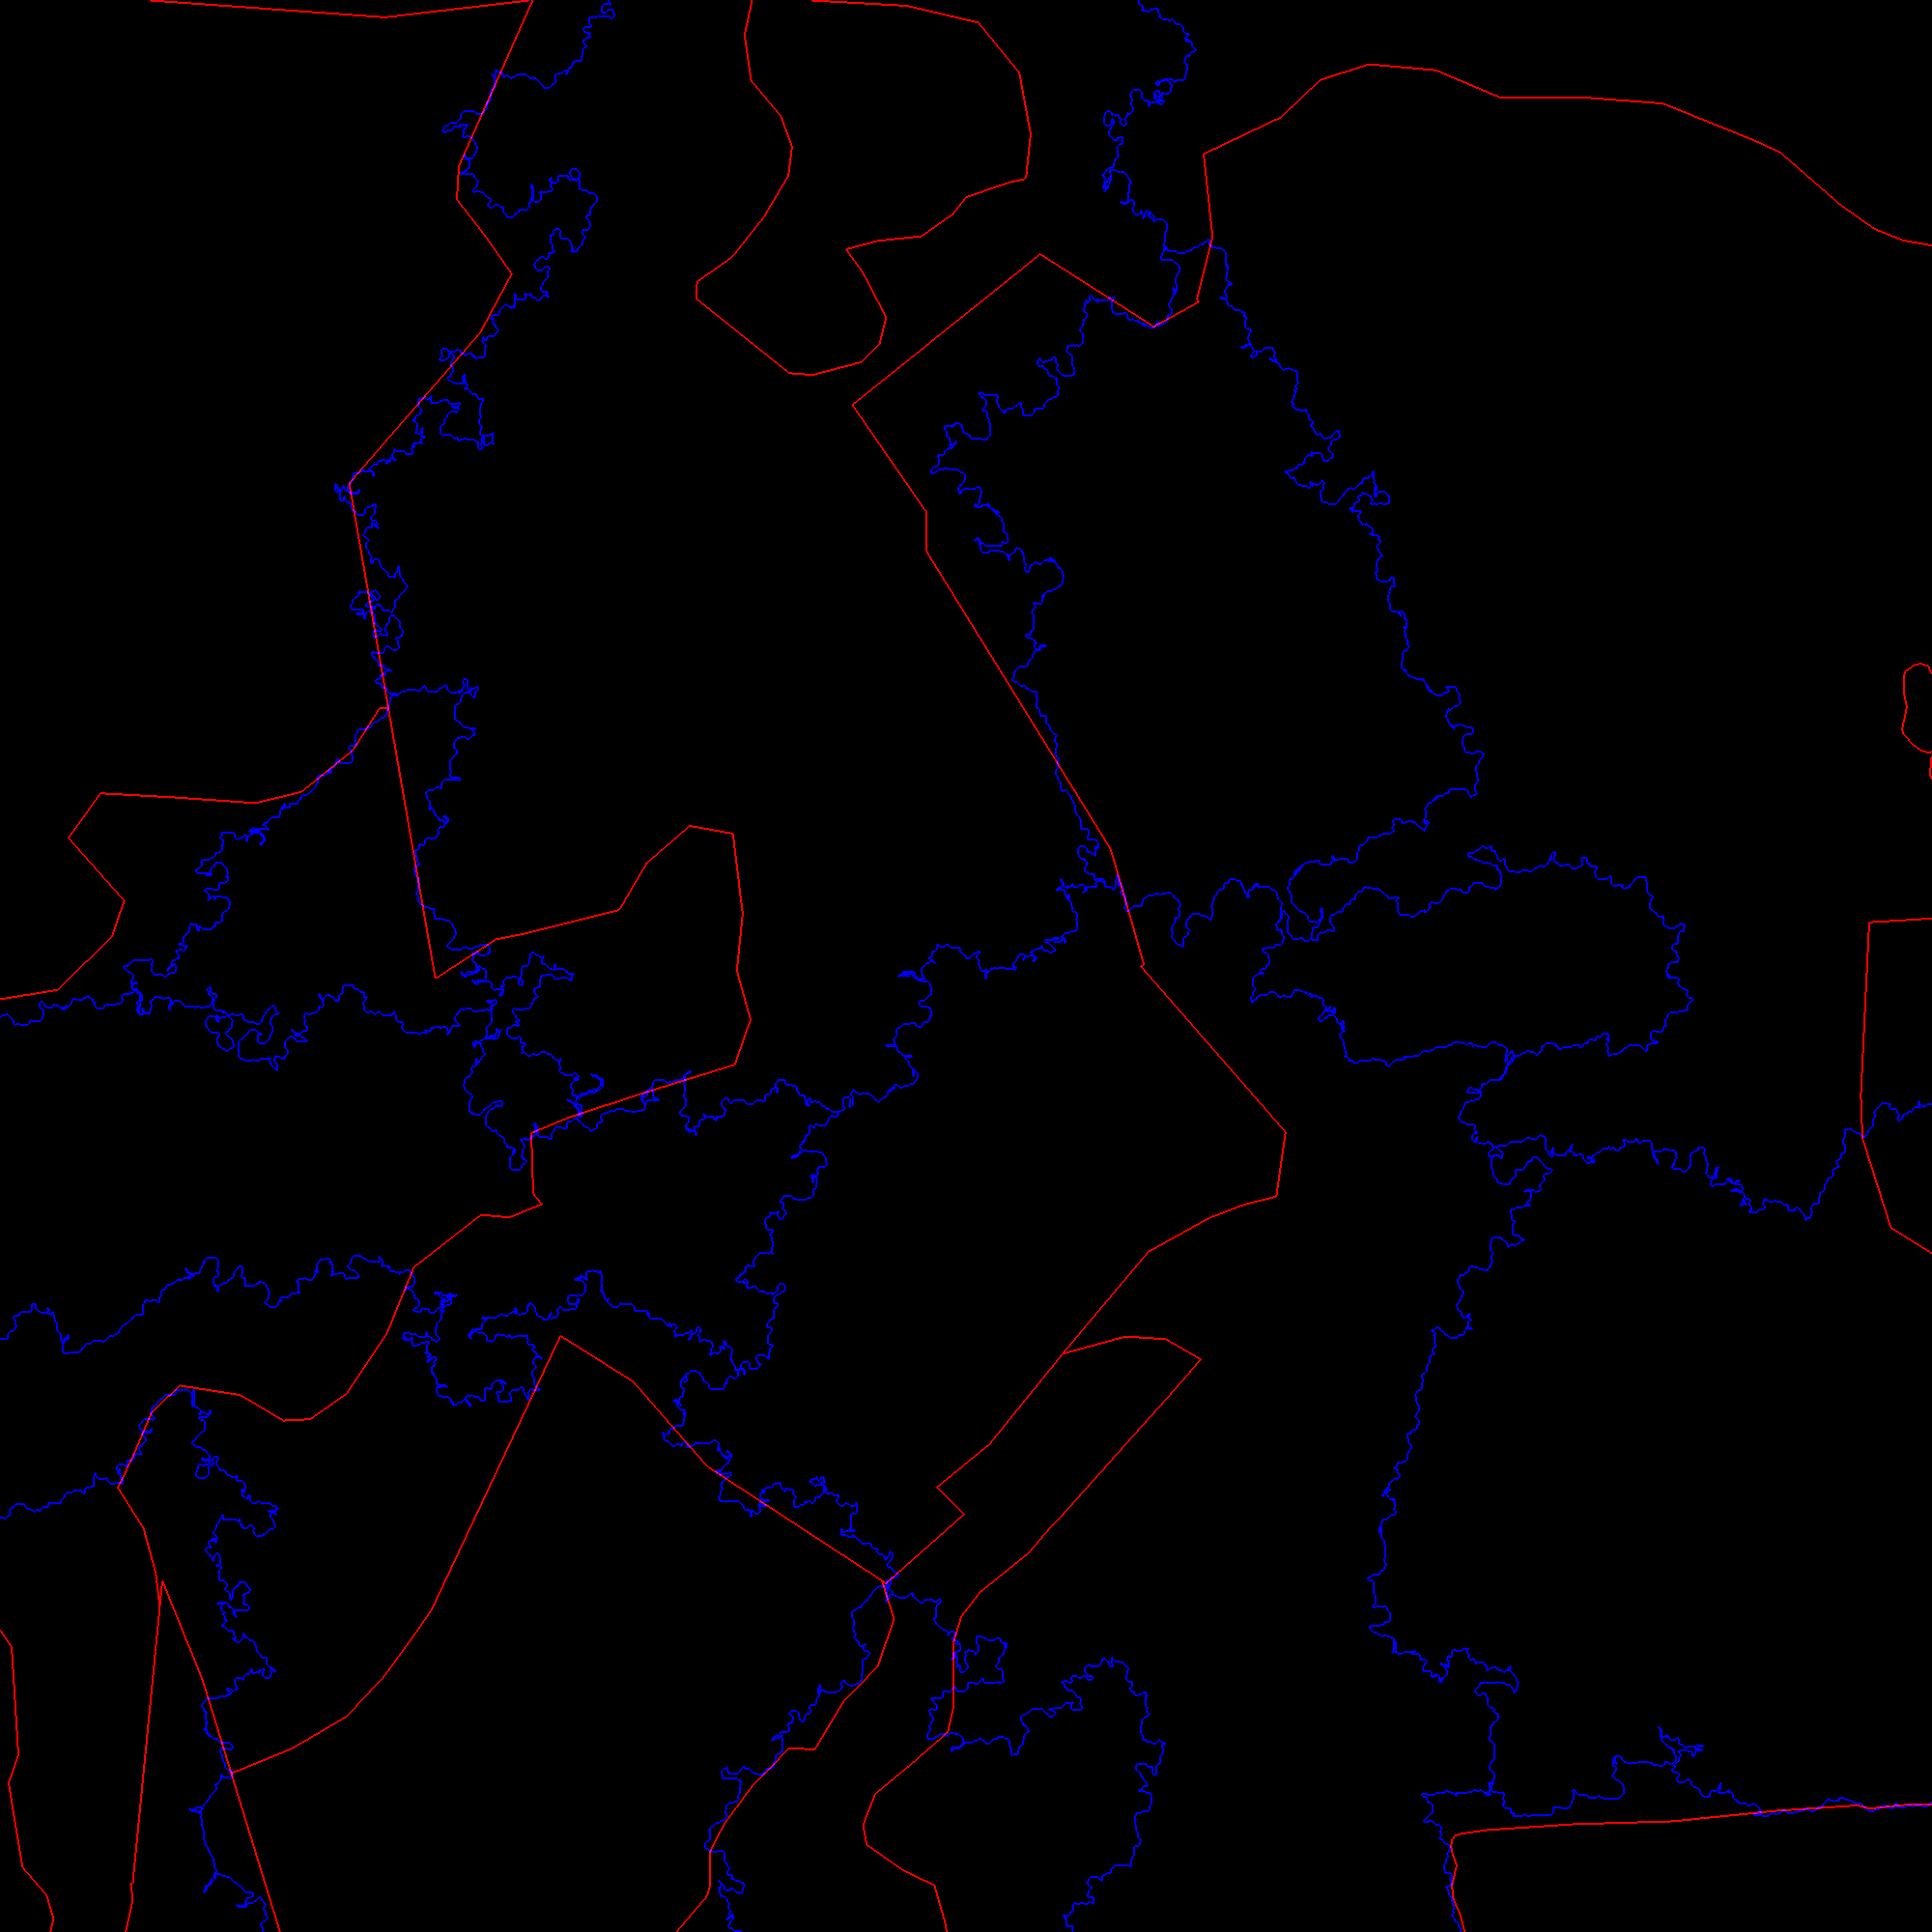
\includegraphics[width=0.45\textwidth]{Figures/C3/S2/border_PFF_z}
\label{subfig:seg_nDSMb}
}
\endgroup
\caption{Result of the segmentation of the nDSM for the two segmentation algorithms. Blue lines correspond to the borders of the segments, red lines correspond to the borders of the forest LC.}
\label{fig:seg_nDSM}
\end{center}
\end{figure}

Since the segmentation on the VHR optical image and the nDSM does not allow to retrieve the borders from the forest LC database, different values of the parameter $\mu$ for the hierarchical segmentation on the VHR optical images (see Figure~\ref{fig:hierar}). It appears that decreasing $\mu$ does not allow to obtain the borders of the forest LC. It only leads to and over-segmentation of the image. Such over-segmentation is employed in the proposed method but is not employed as a relevant segmentation for stand delineation but as an input for object based classification.

\begin{figure}[htbp]
\begin{center}
\begingroup
\captionsetup[subfigure]{width=0.5\textwidth}
\subfloat[Hierarchical segmentation with $\mu=3$.]{
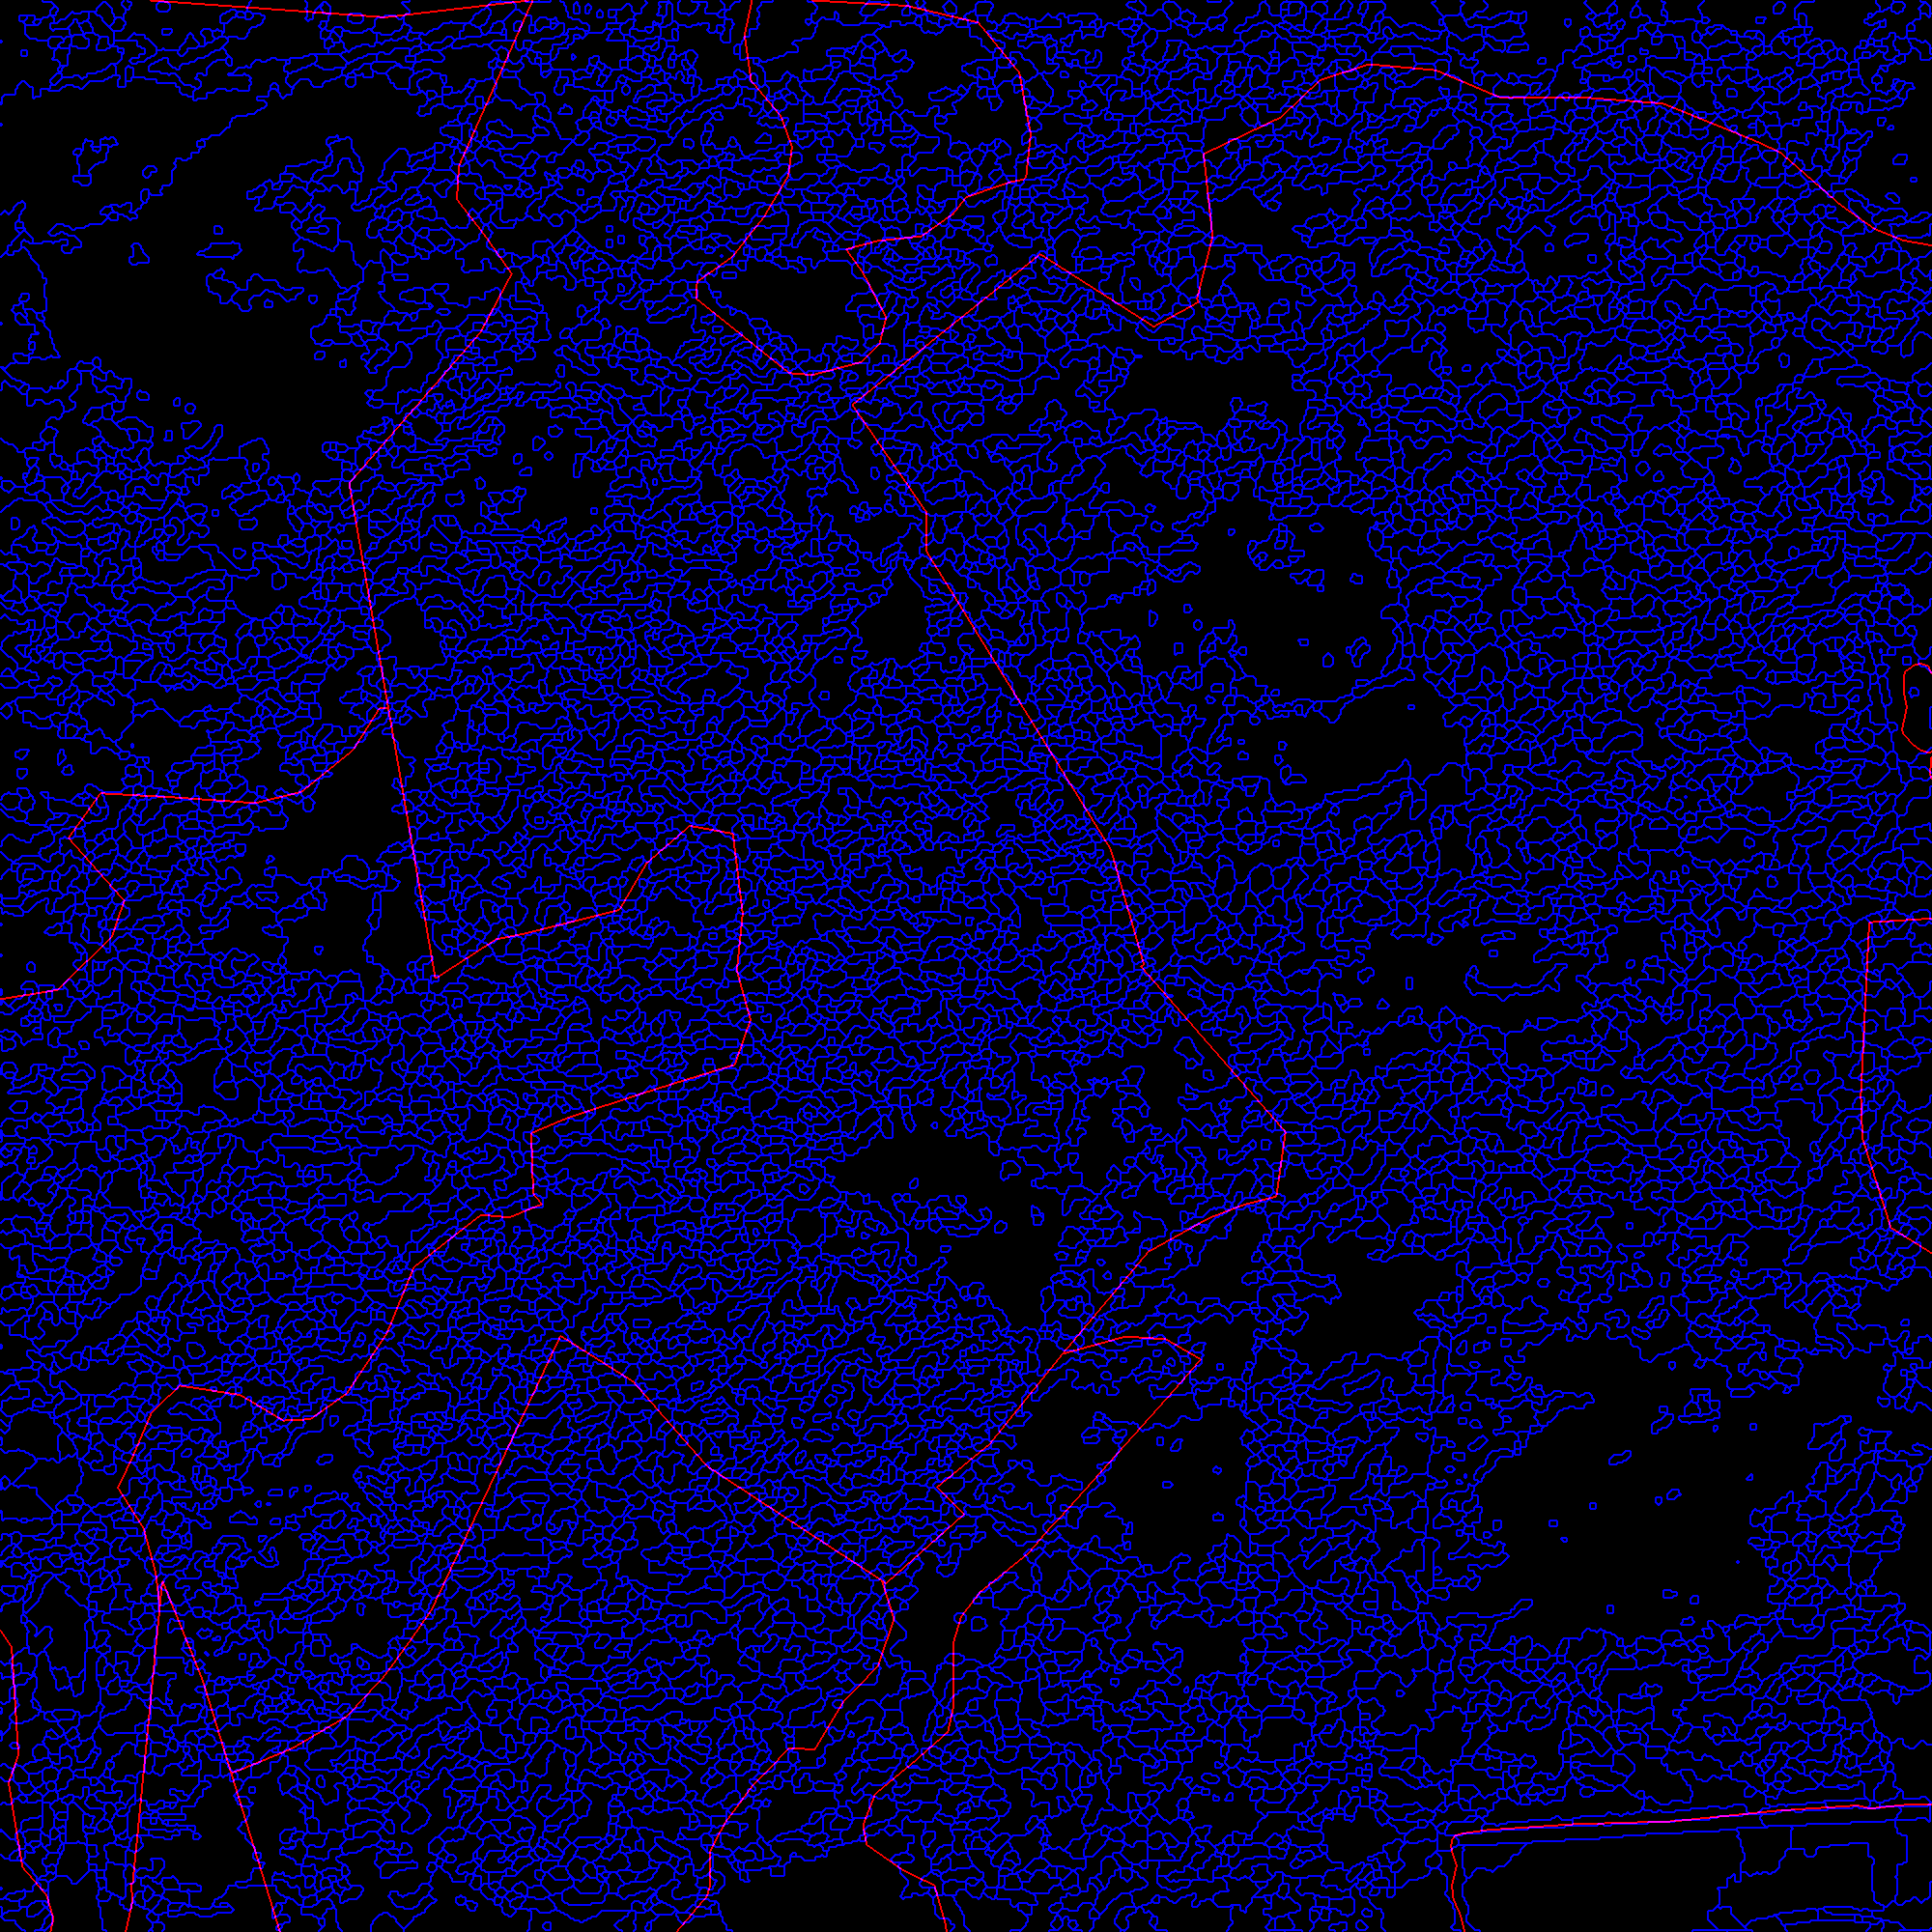
\includegraphics[width=0.45\textwidth]{Figures/C3/S2/seg_herarchical_3border_hierarchical}
\label{subfig:hierar3}
}
\hspace*{0.05\textwidth}
\subfloat[Hierarchical segmentation with $\mu=6$.]{
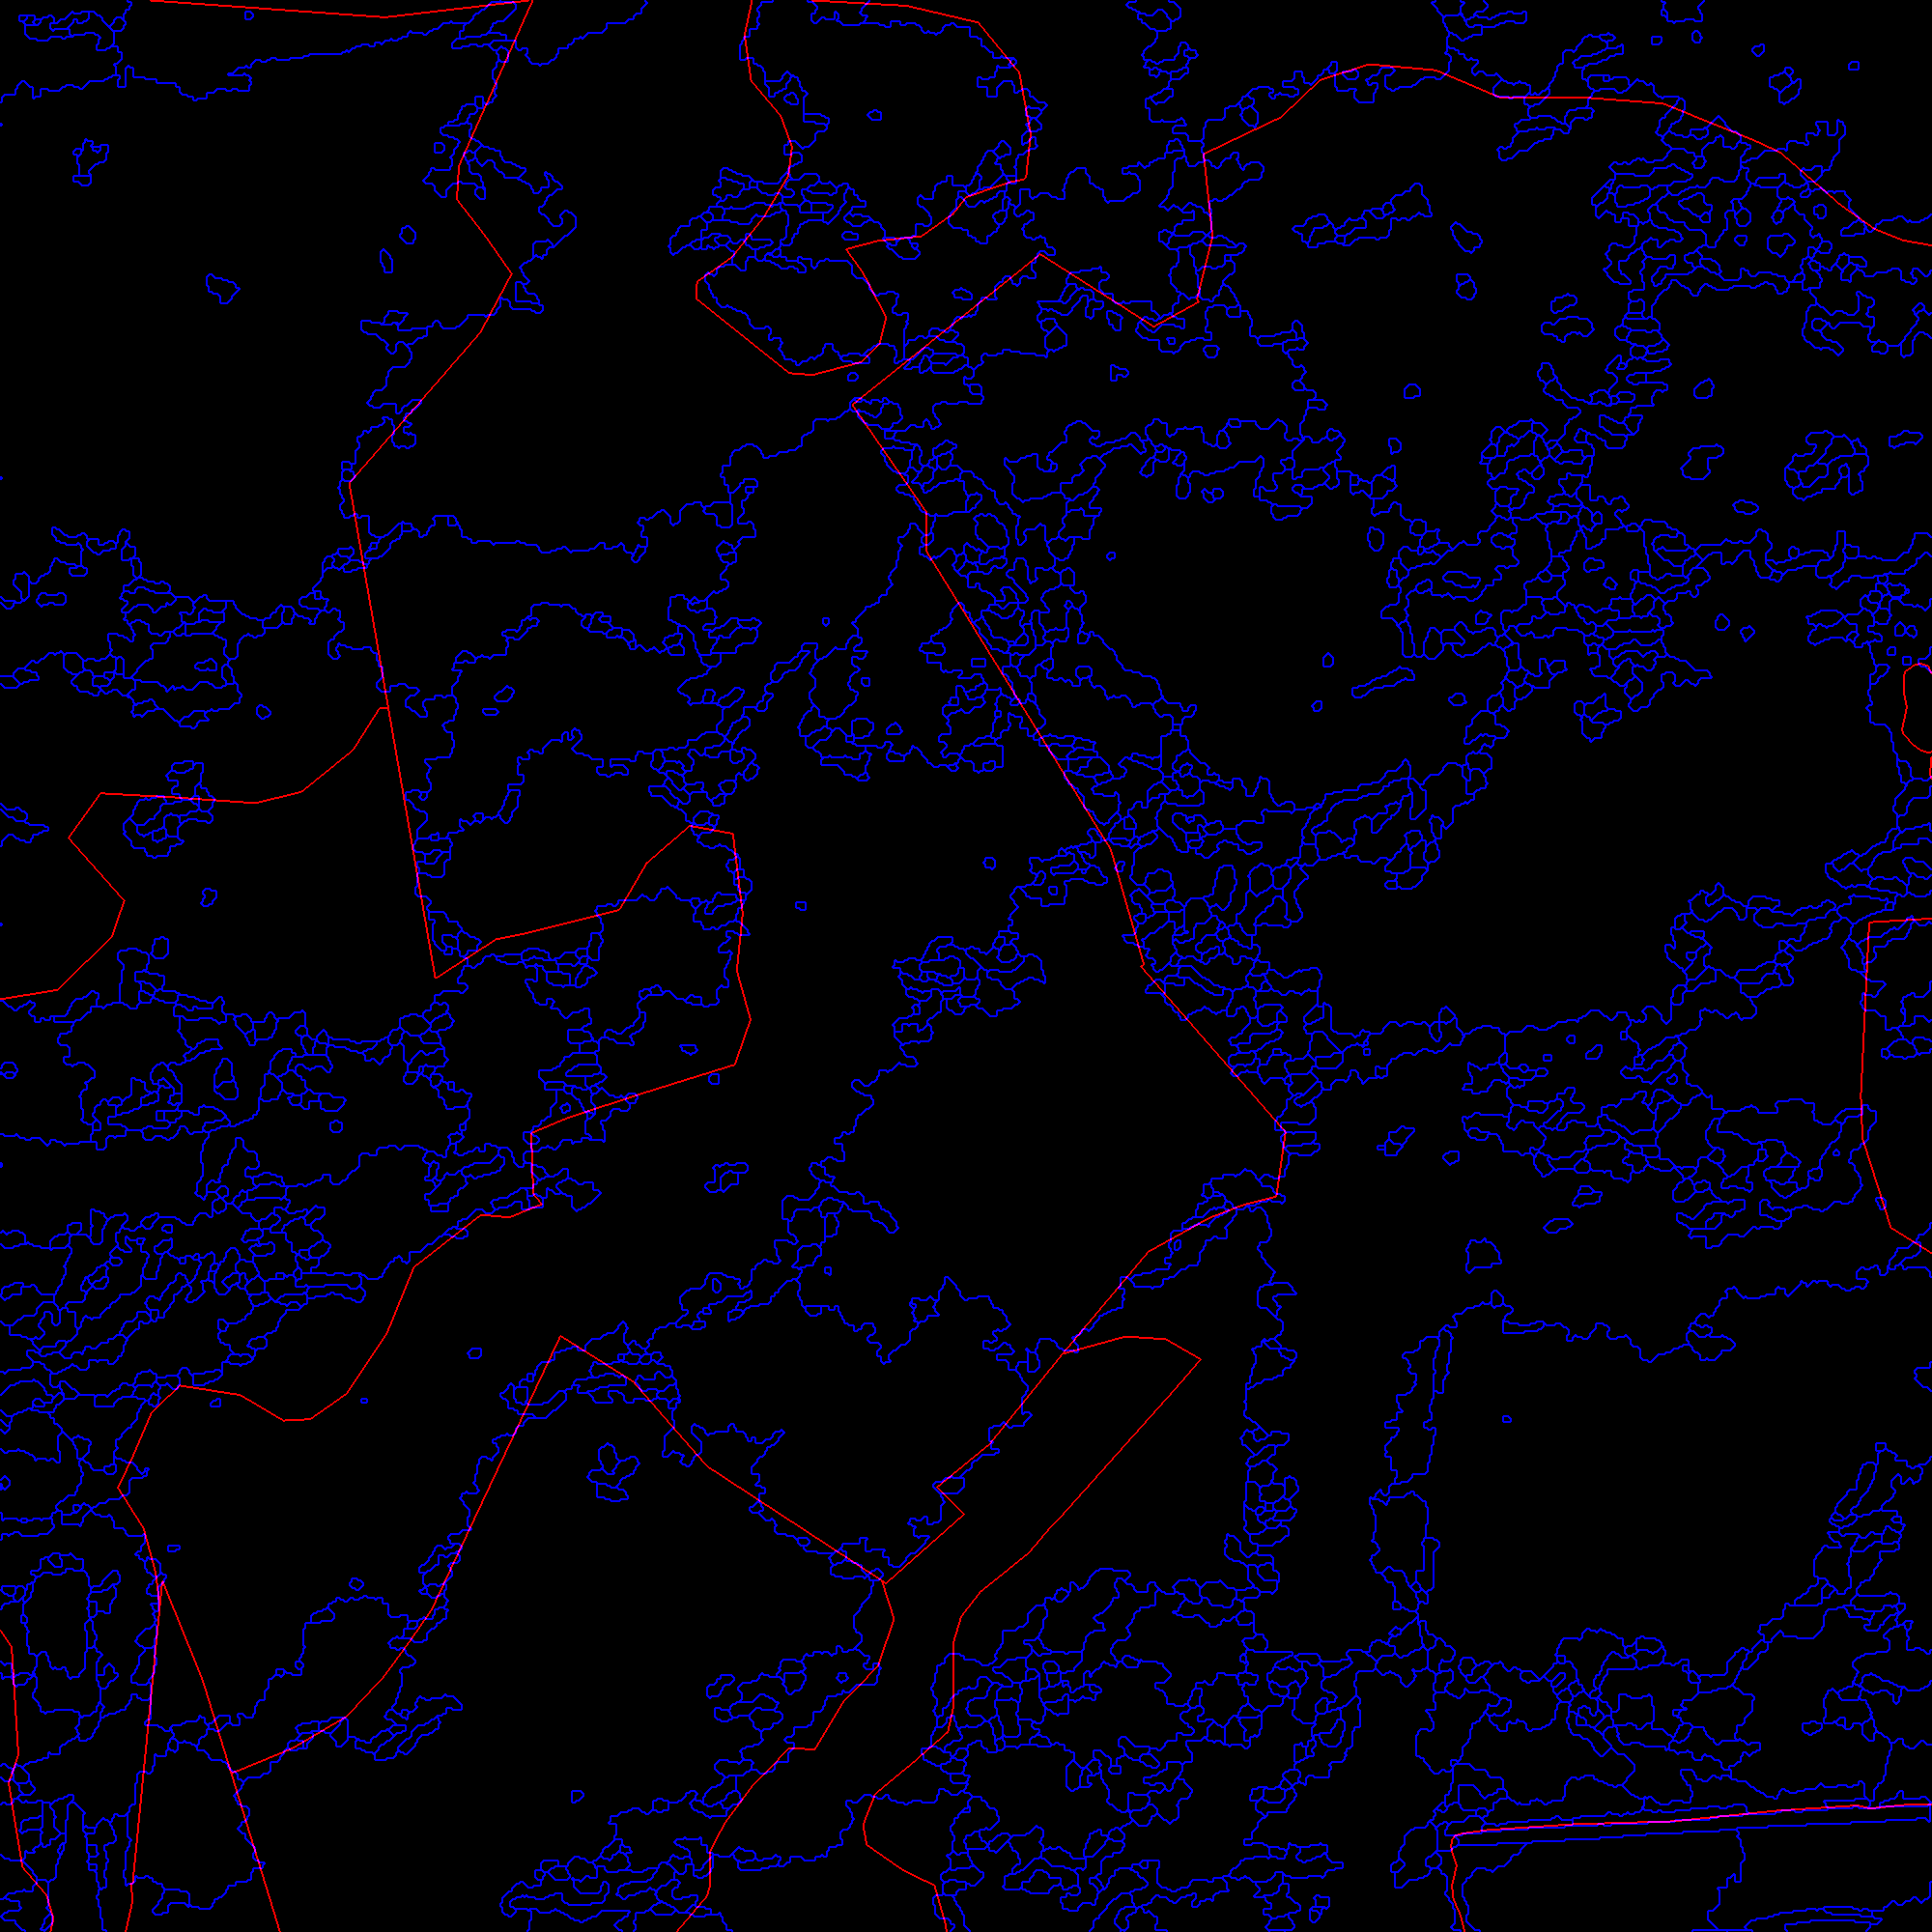
\includegraphics[width=0.45\textwidth]{Figures/C3/S2/seg_herarchical_6border_hierarchical}
\label{subfig:hierar6}
}
\\
\subfloat[Hierarchical segmentation with $\mu=8$.]{
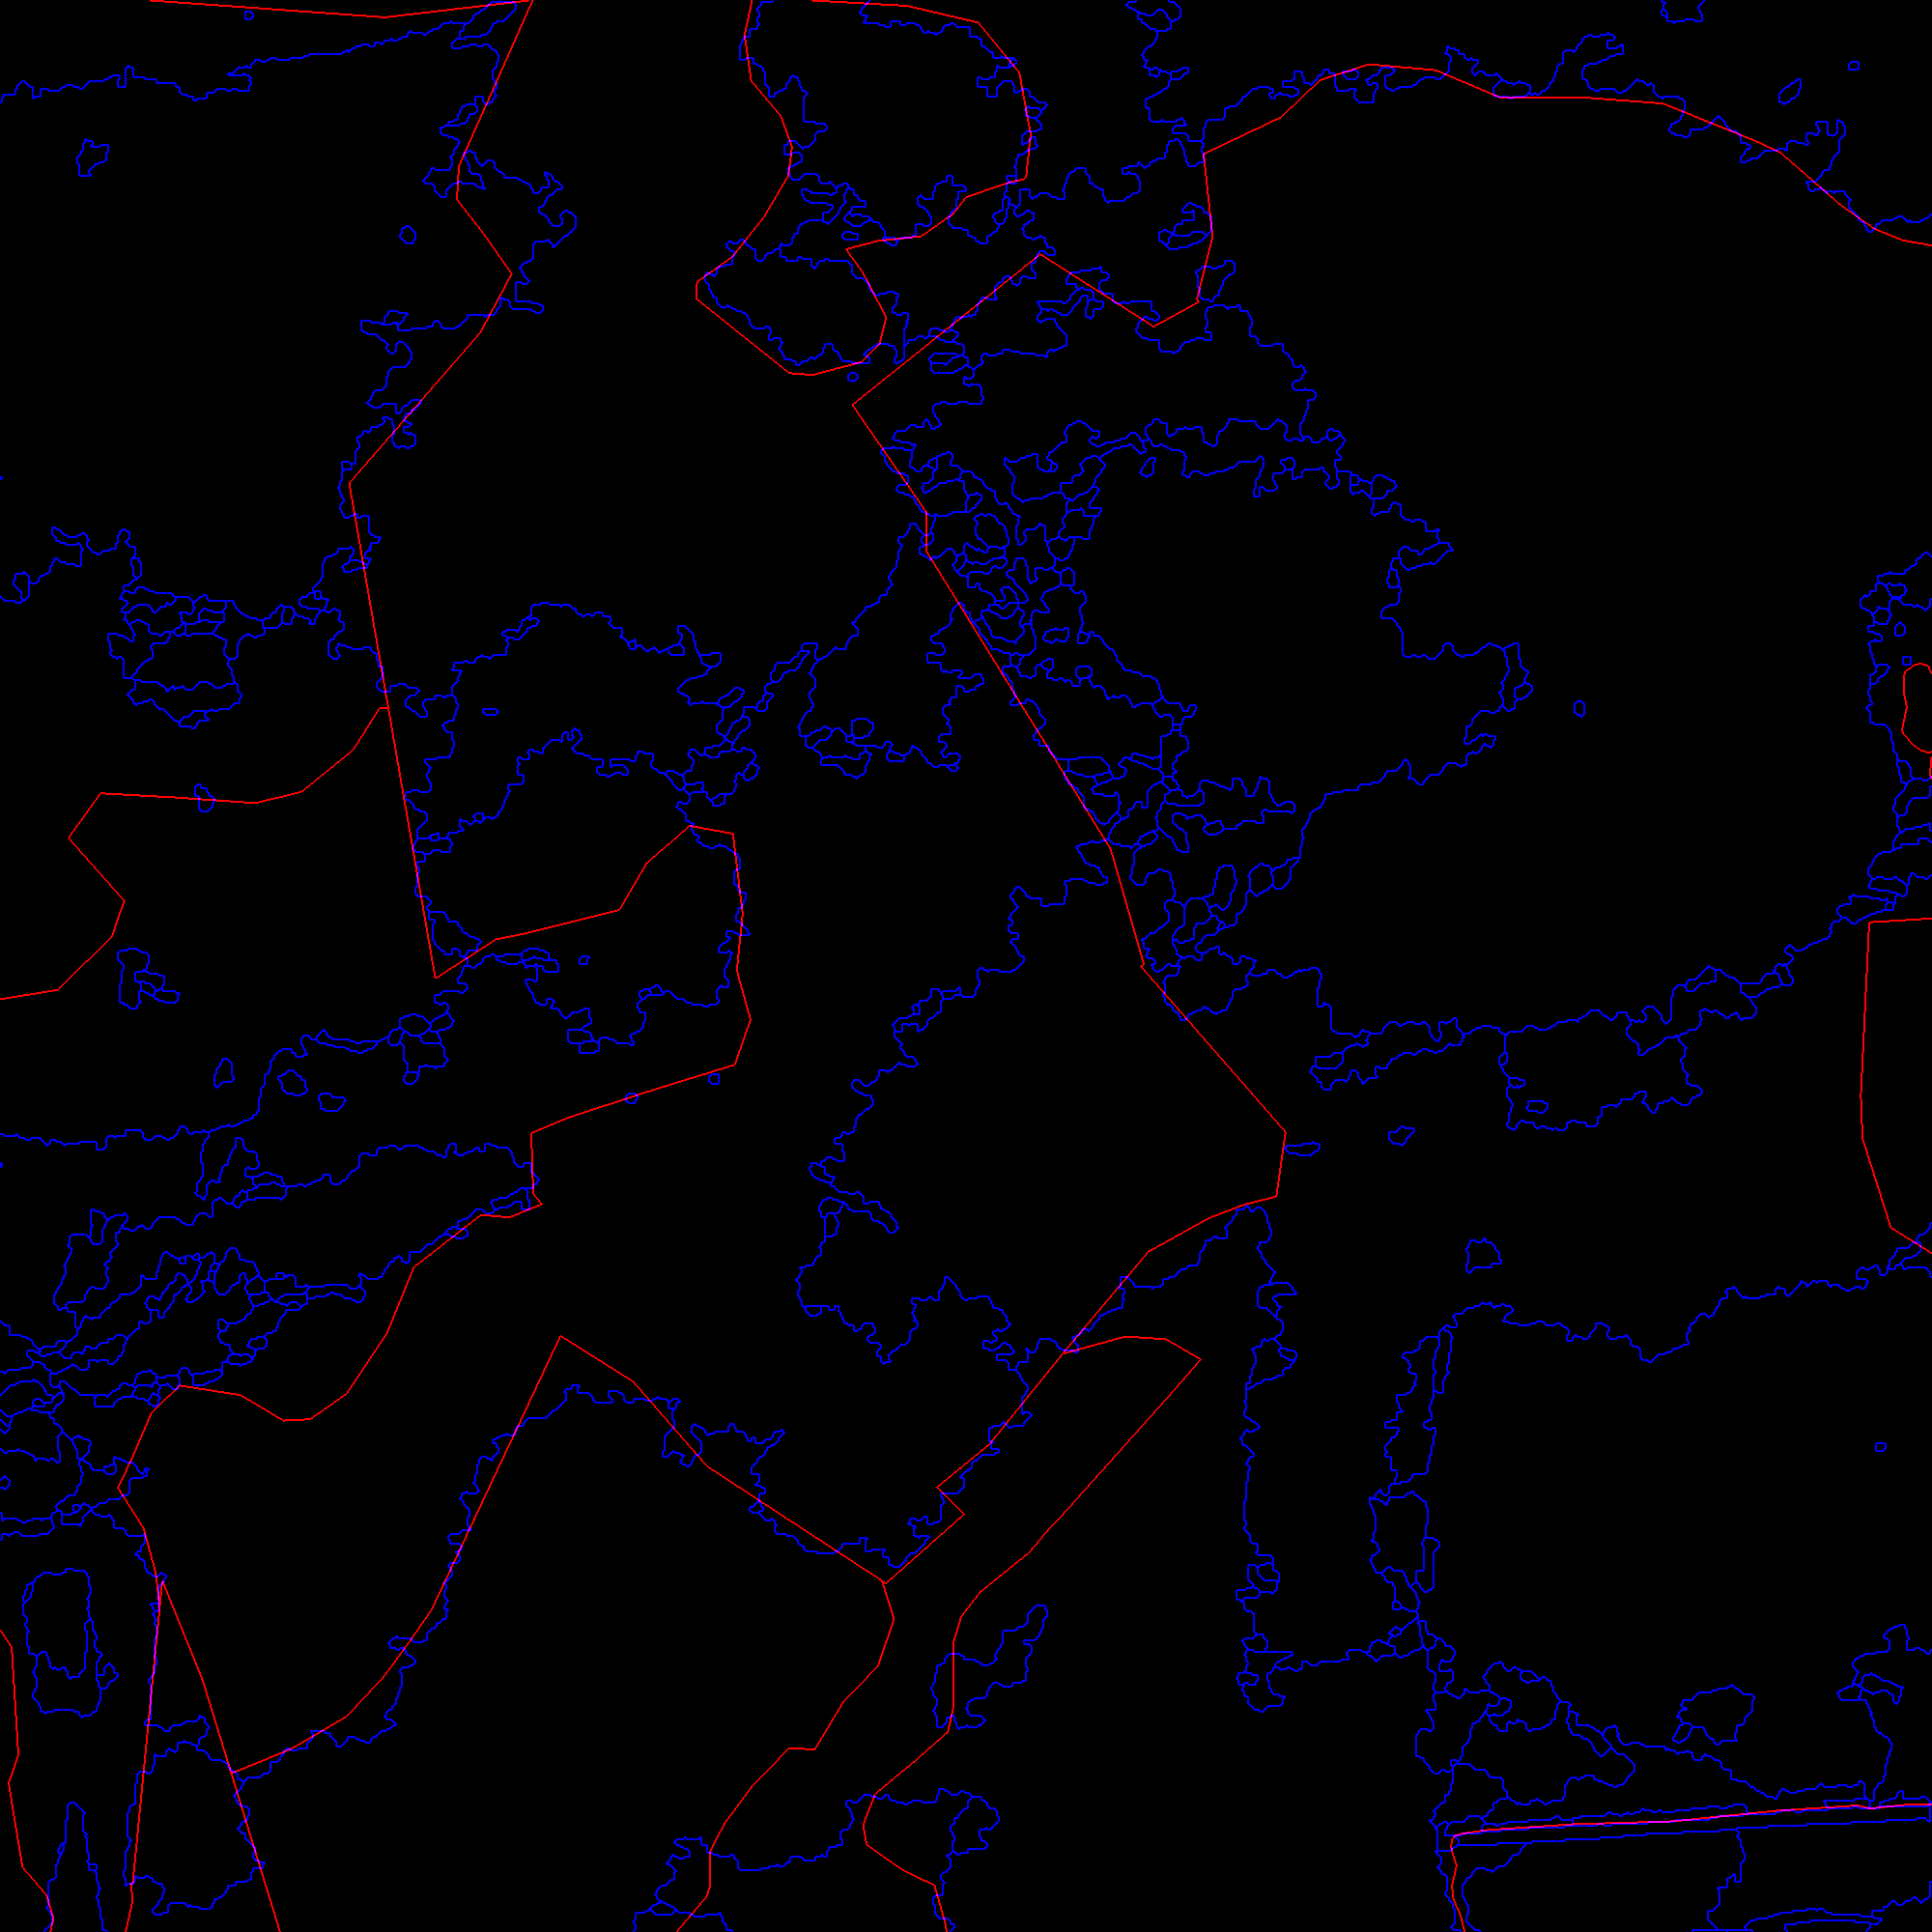
\includegraphics[width=0.45\textwidth]{Figures/C3/S2/seg_herarchical_8border_hierarchical}
\label{subfig:hierar8}
}
\hspace*{0.05\textwidth}
\subfloat[Hierarchical segmentation with $\mu=10$.]{
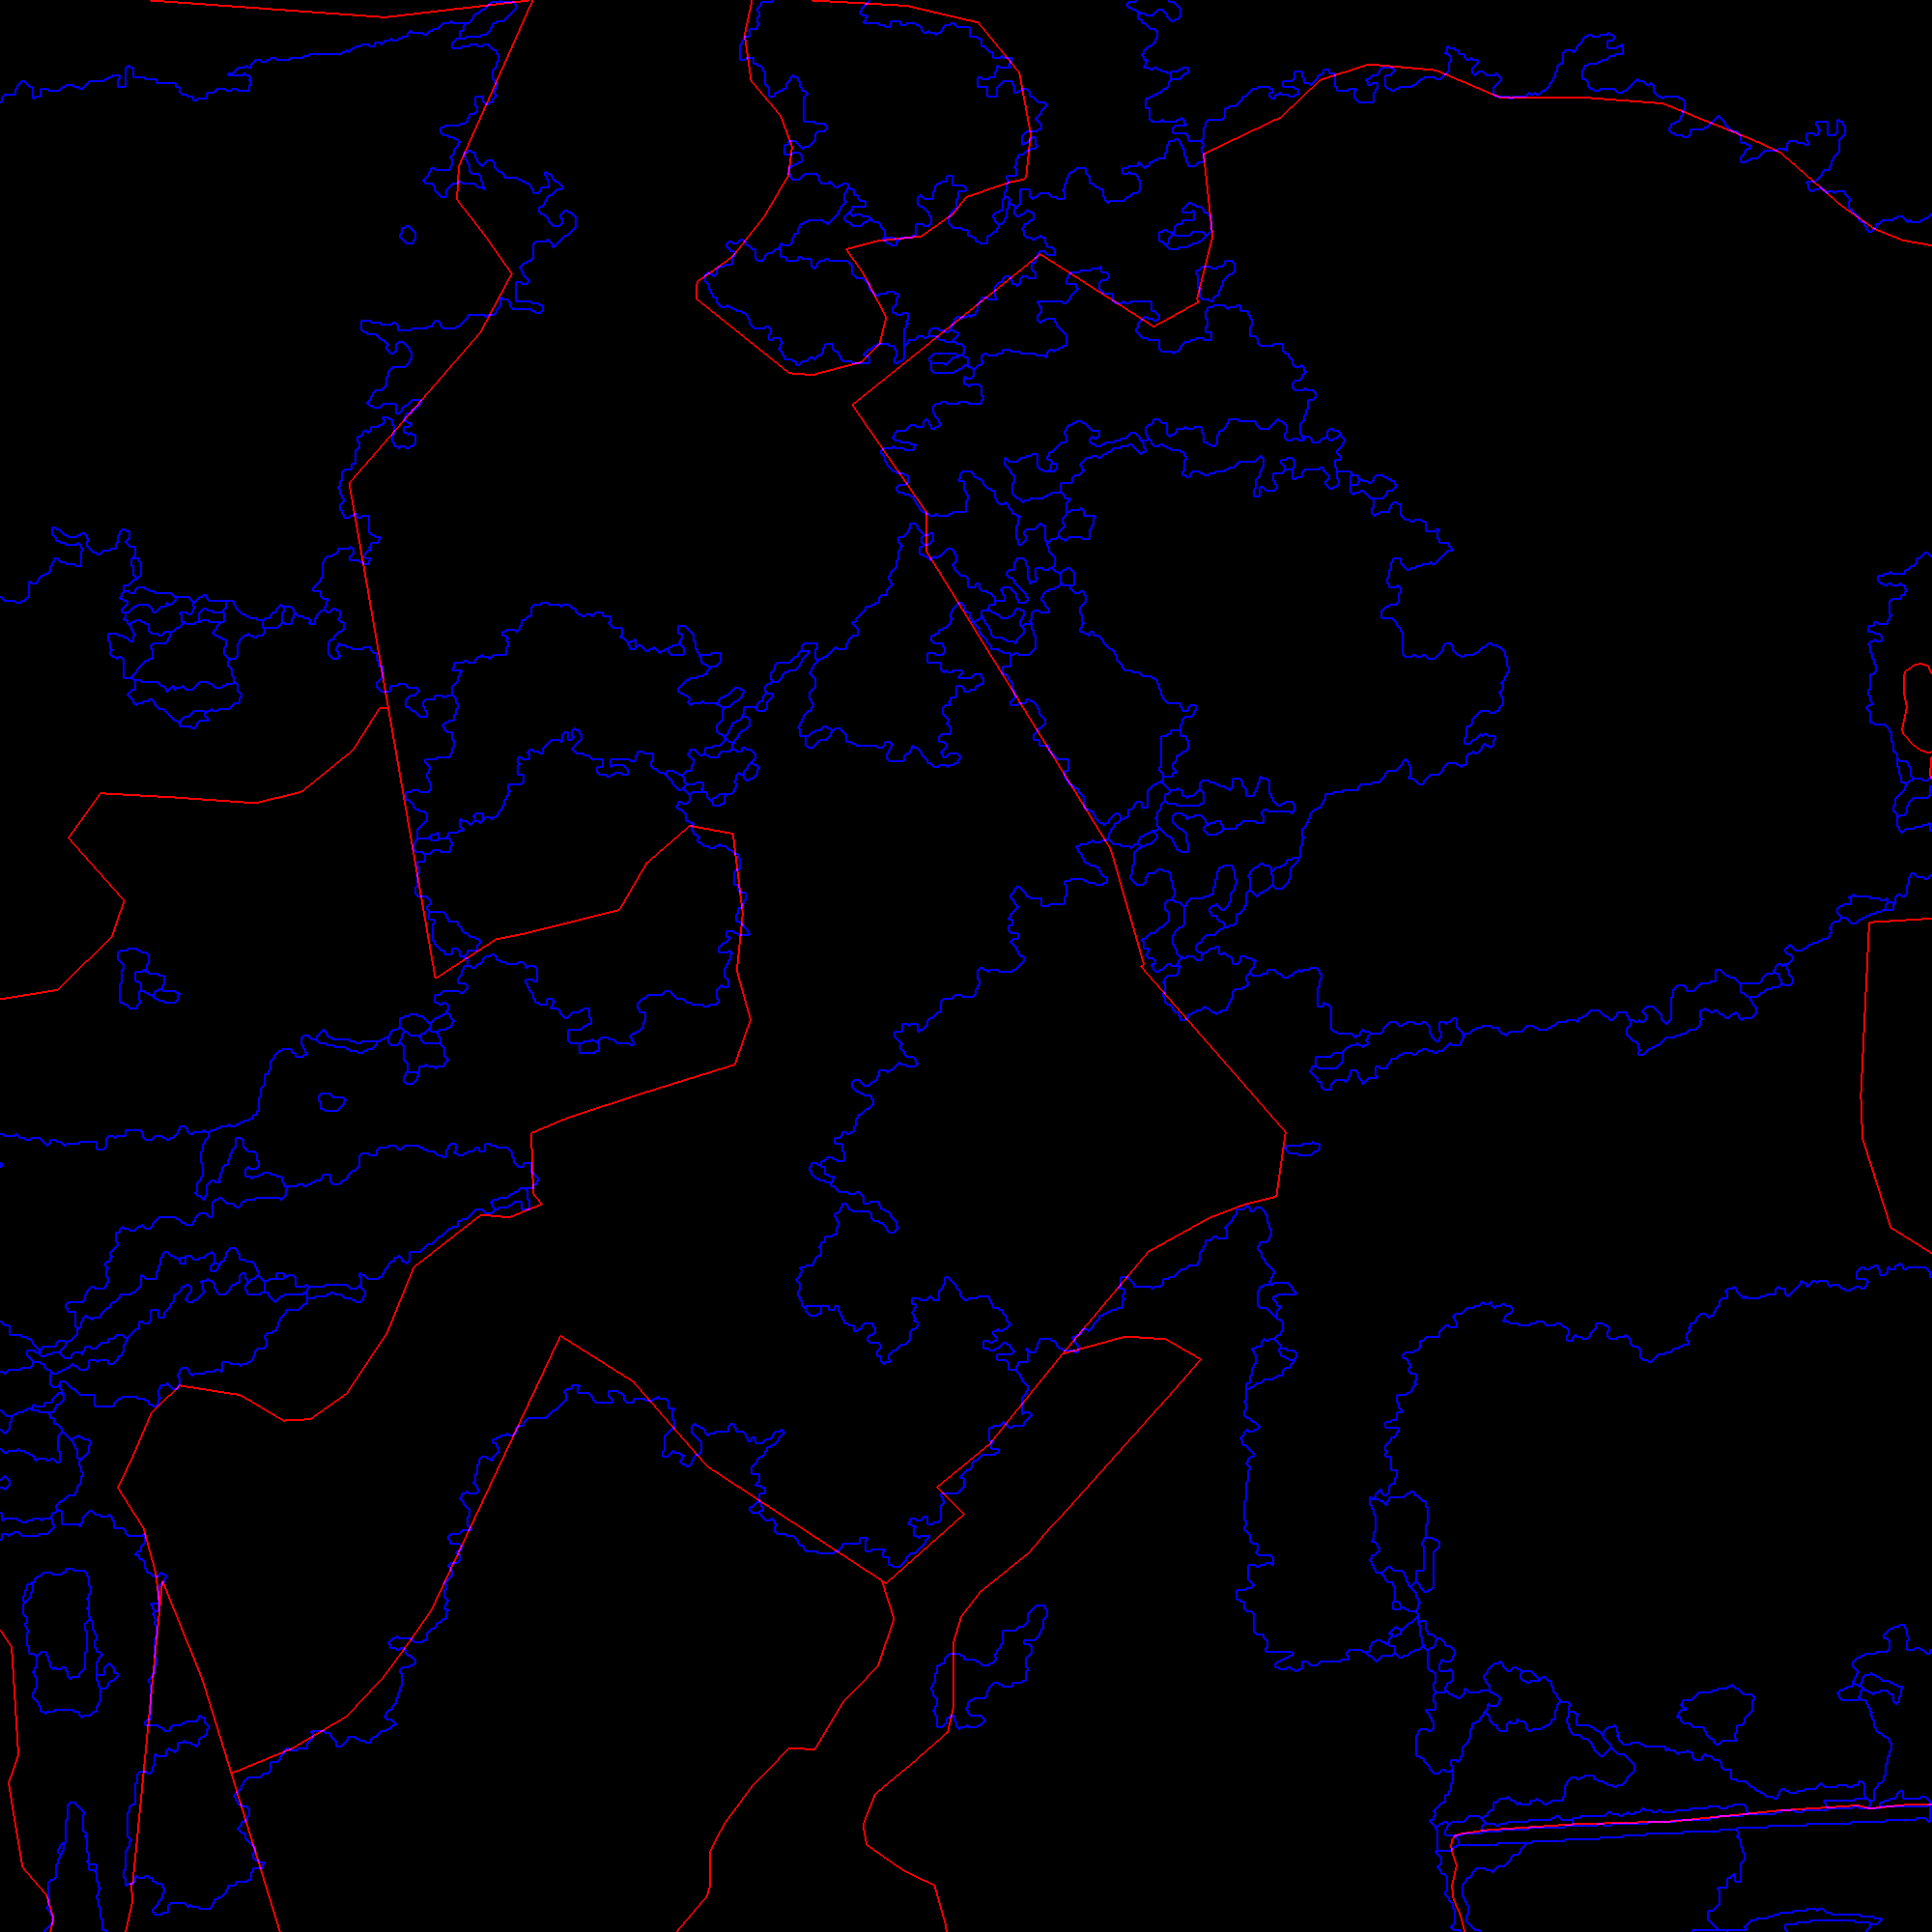
\includegraphics[width=0.45\textwidth]{Figures/C3/S2/seg_herarchical_10border_hierarchical}
\label{subfig:hierar10}
}
\\
\subfloat[Hierarchical segmentation with $\mu=12$.]{
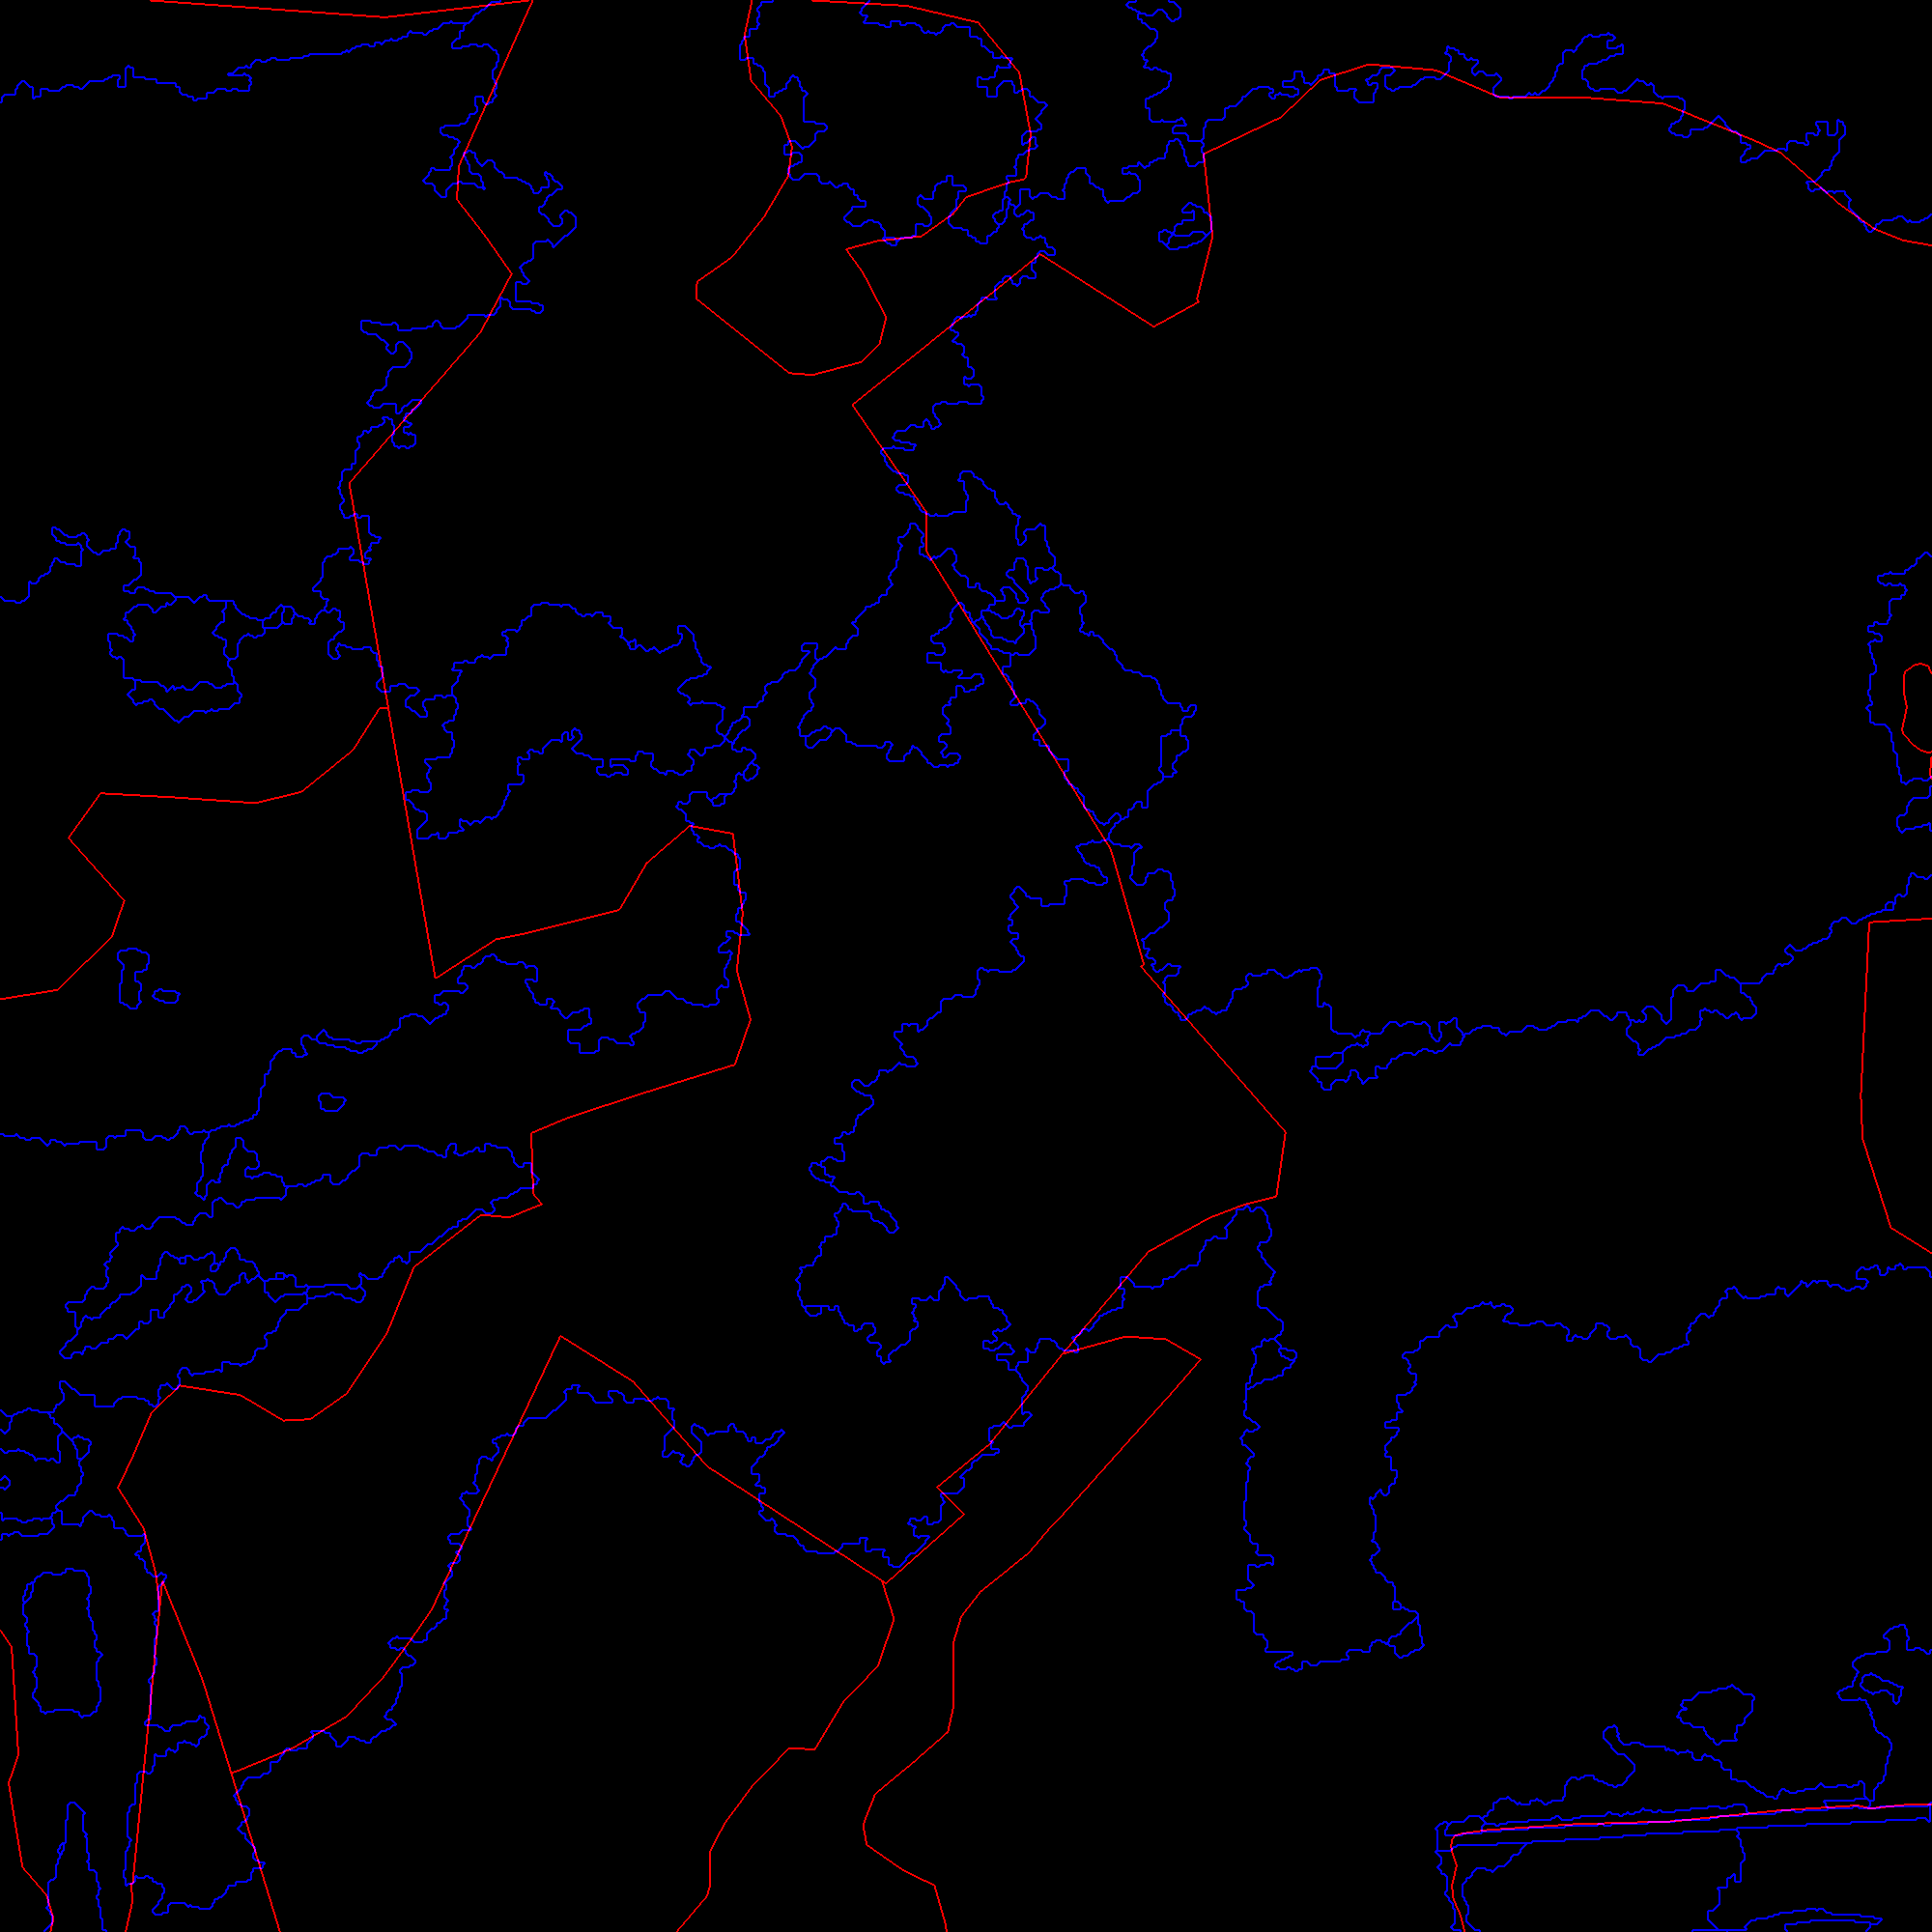
\includegraphics[width=0.45\textwidth]{Figures/C3/S2/seg_herarchical_12border_hierarchical}
\label{subfig:hierar12}
}
\hspace*{0.05\textwidth}
\subfloat[Hierarchical segmentation with $\mu=15$.]{
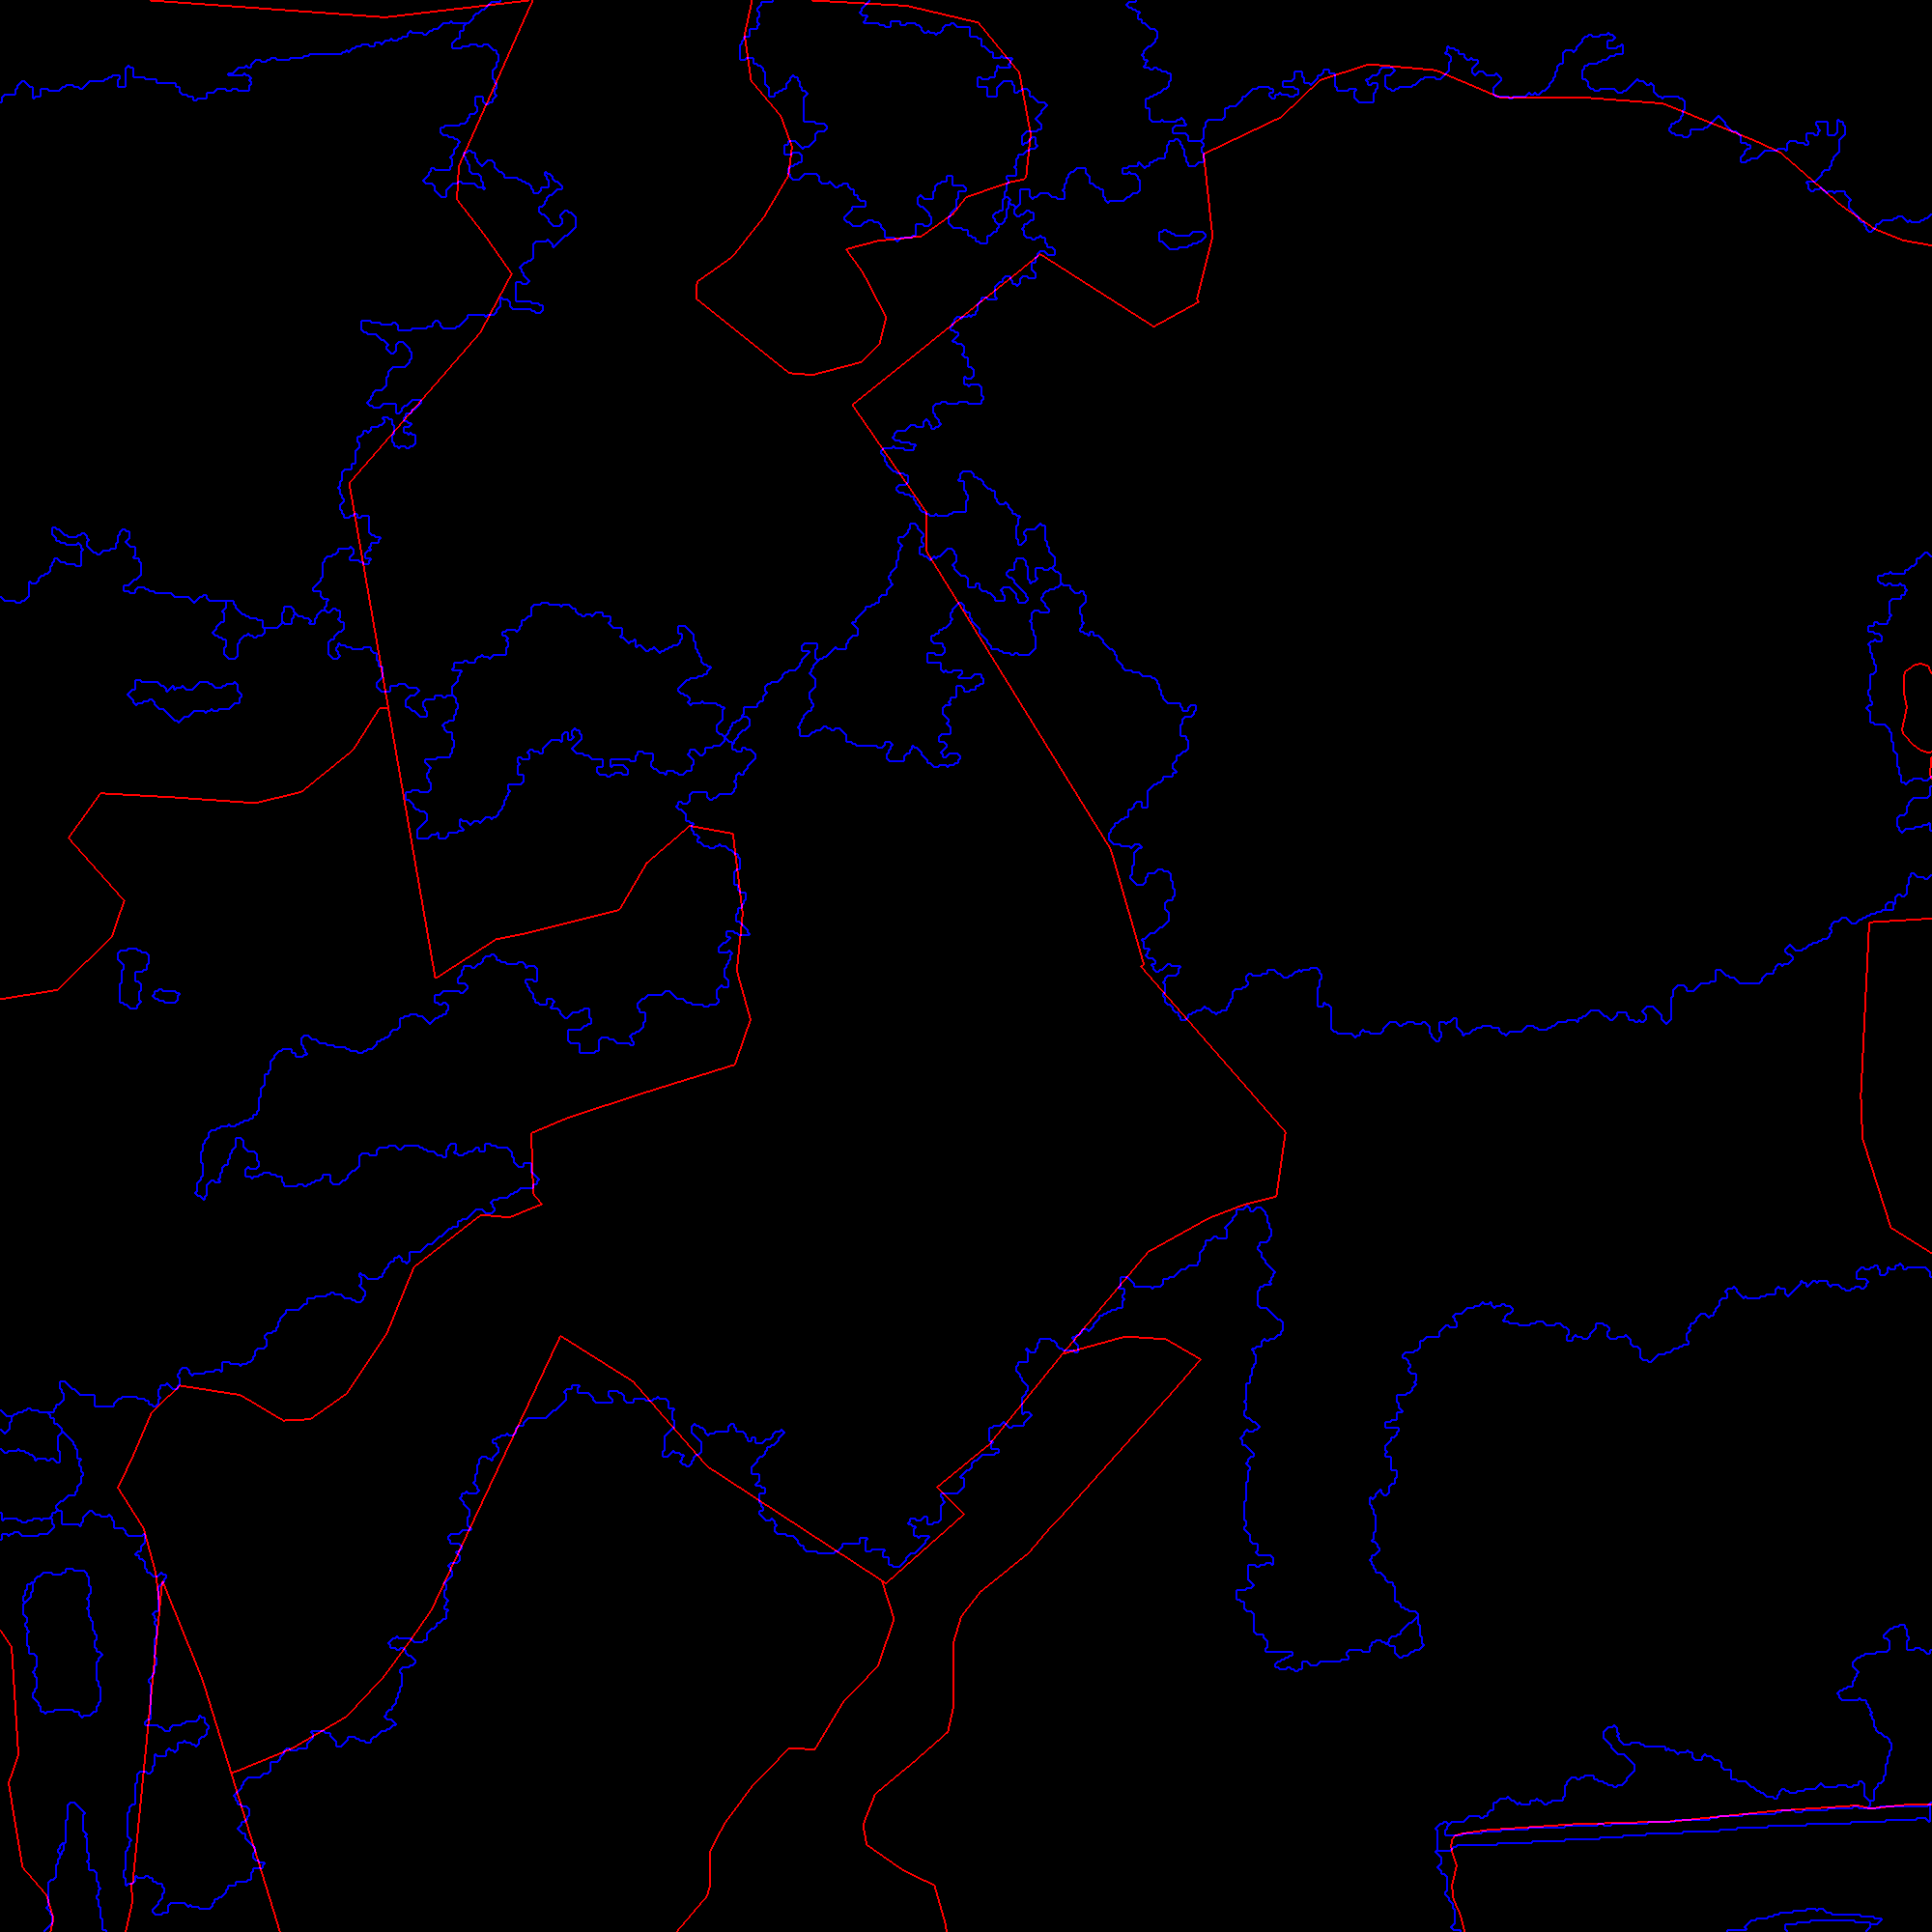
\includegraphics[width=0.45\textwidth]{Figures/C3/S2/seg_herarchical_15border_hierarchical}
\label{subfig:hierar15}
}
\endgroup
\caption{Result of the segmentation of the VHR optical image using different values of $\mu$ for the hierarchical segmentation. Blue lines correspond to the borders of the segments, red lines correspond to the borders of the forest LC.}
\label{fig:hierar}
\end{center}
\end{figure}

The two proposed segmentation algorithms are very efficient for image segmentation tasks \citep{guigues2006scale, felzenszwalb2004efficient} but are not adapted to retrieve forest stands borders. However, they can produce interesting over-segmentation since they are able to retrieve some relevant borders.

\subsection{Add semantic information}
The classification proposed in the method give information about the species at the object level. Since the segments extracted below are large than the small objects, a majority vote can be applied for each segment. The obtained label map could be compared with the forest LC.
The result of the classification for the area of interest is presented in Figure~\ref{fig:C3_S2_classif}, the confusion matrix and other accuracy metrics for this classification are presented in Table~\ref{table:C3_S2_classif}.

\begin{figure}[htbp]
\begin{center}
\begingroup
\captionsetup[subfigure]{width=0.375\textwidth}
\subfloat[Forest LC.]{
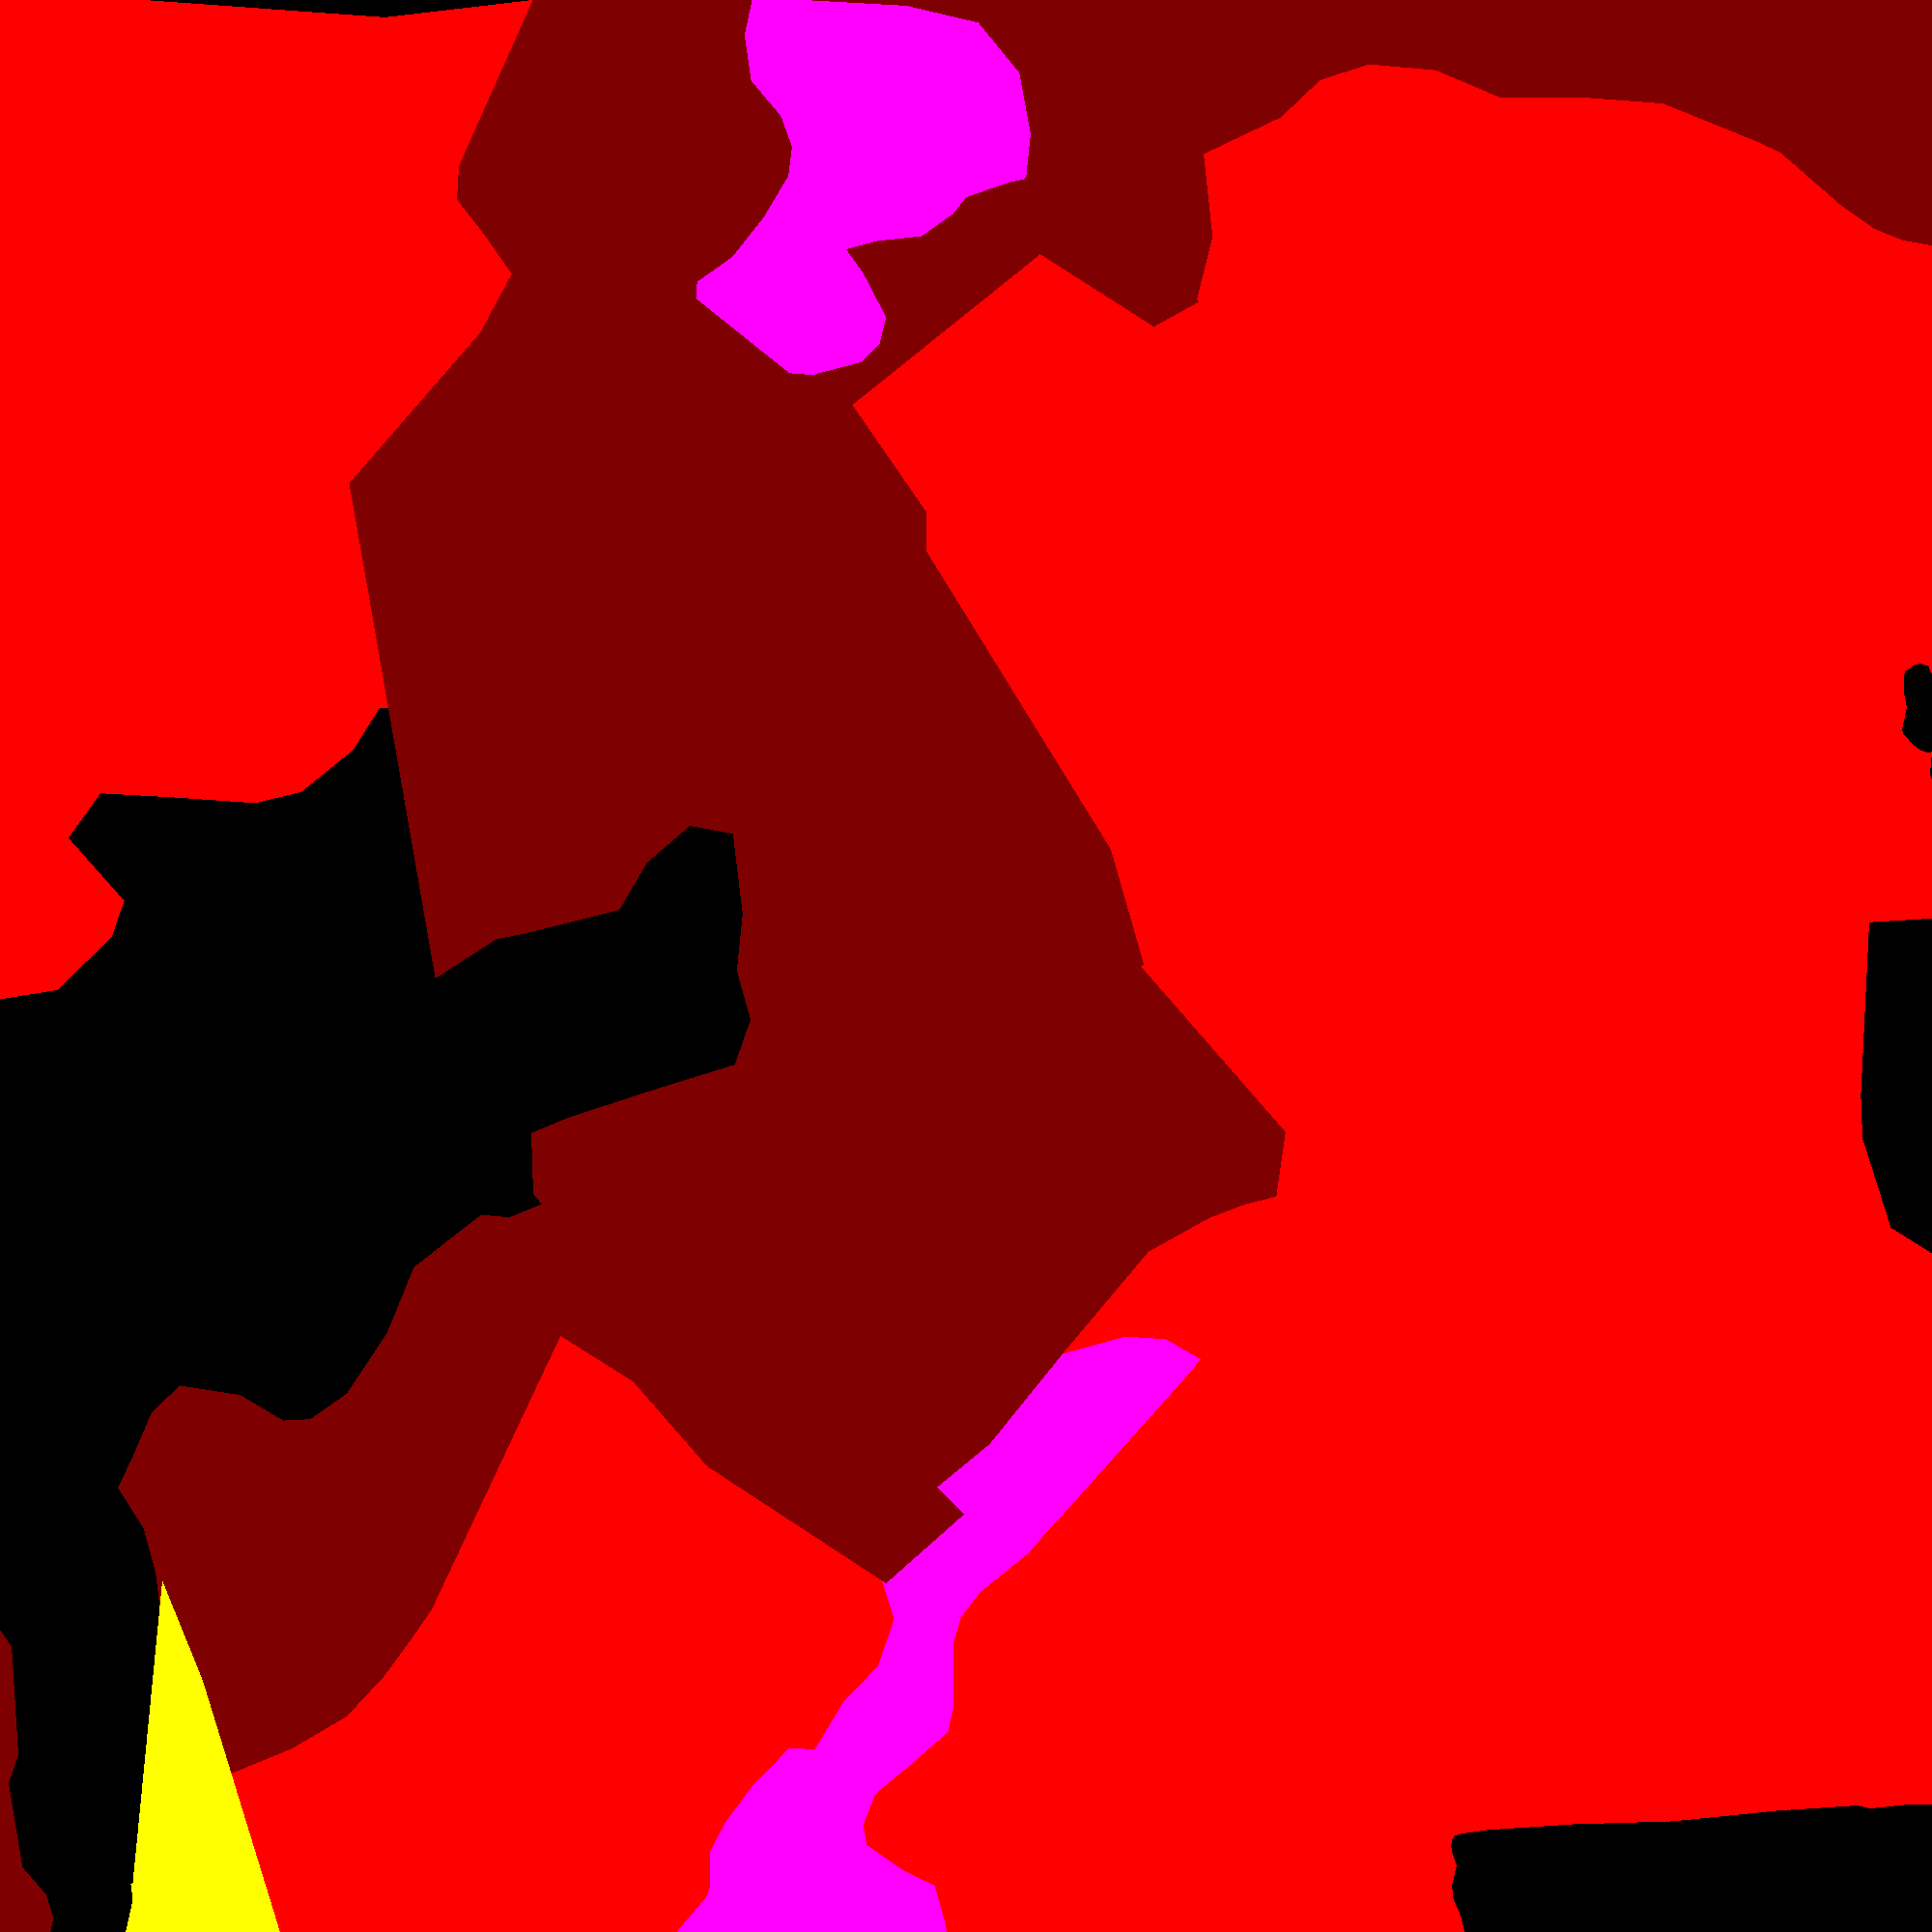
\includegraphics[width=0.45\textwidth]{Figures/C3/S2/BD}
\label{subfig:C3_S2_classifa}
}
\hspace*{0.05\textwidth}
\subfloat[Classification results (overall accuracy: 81.75\%, $\kappa$: 0.67).]{
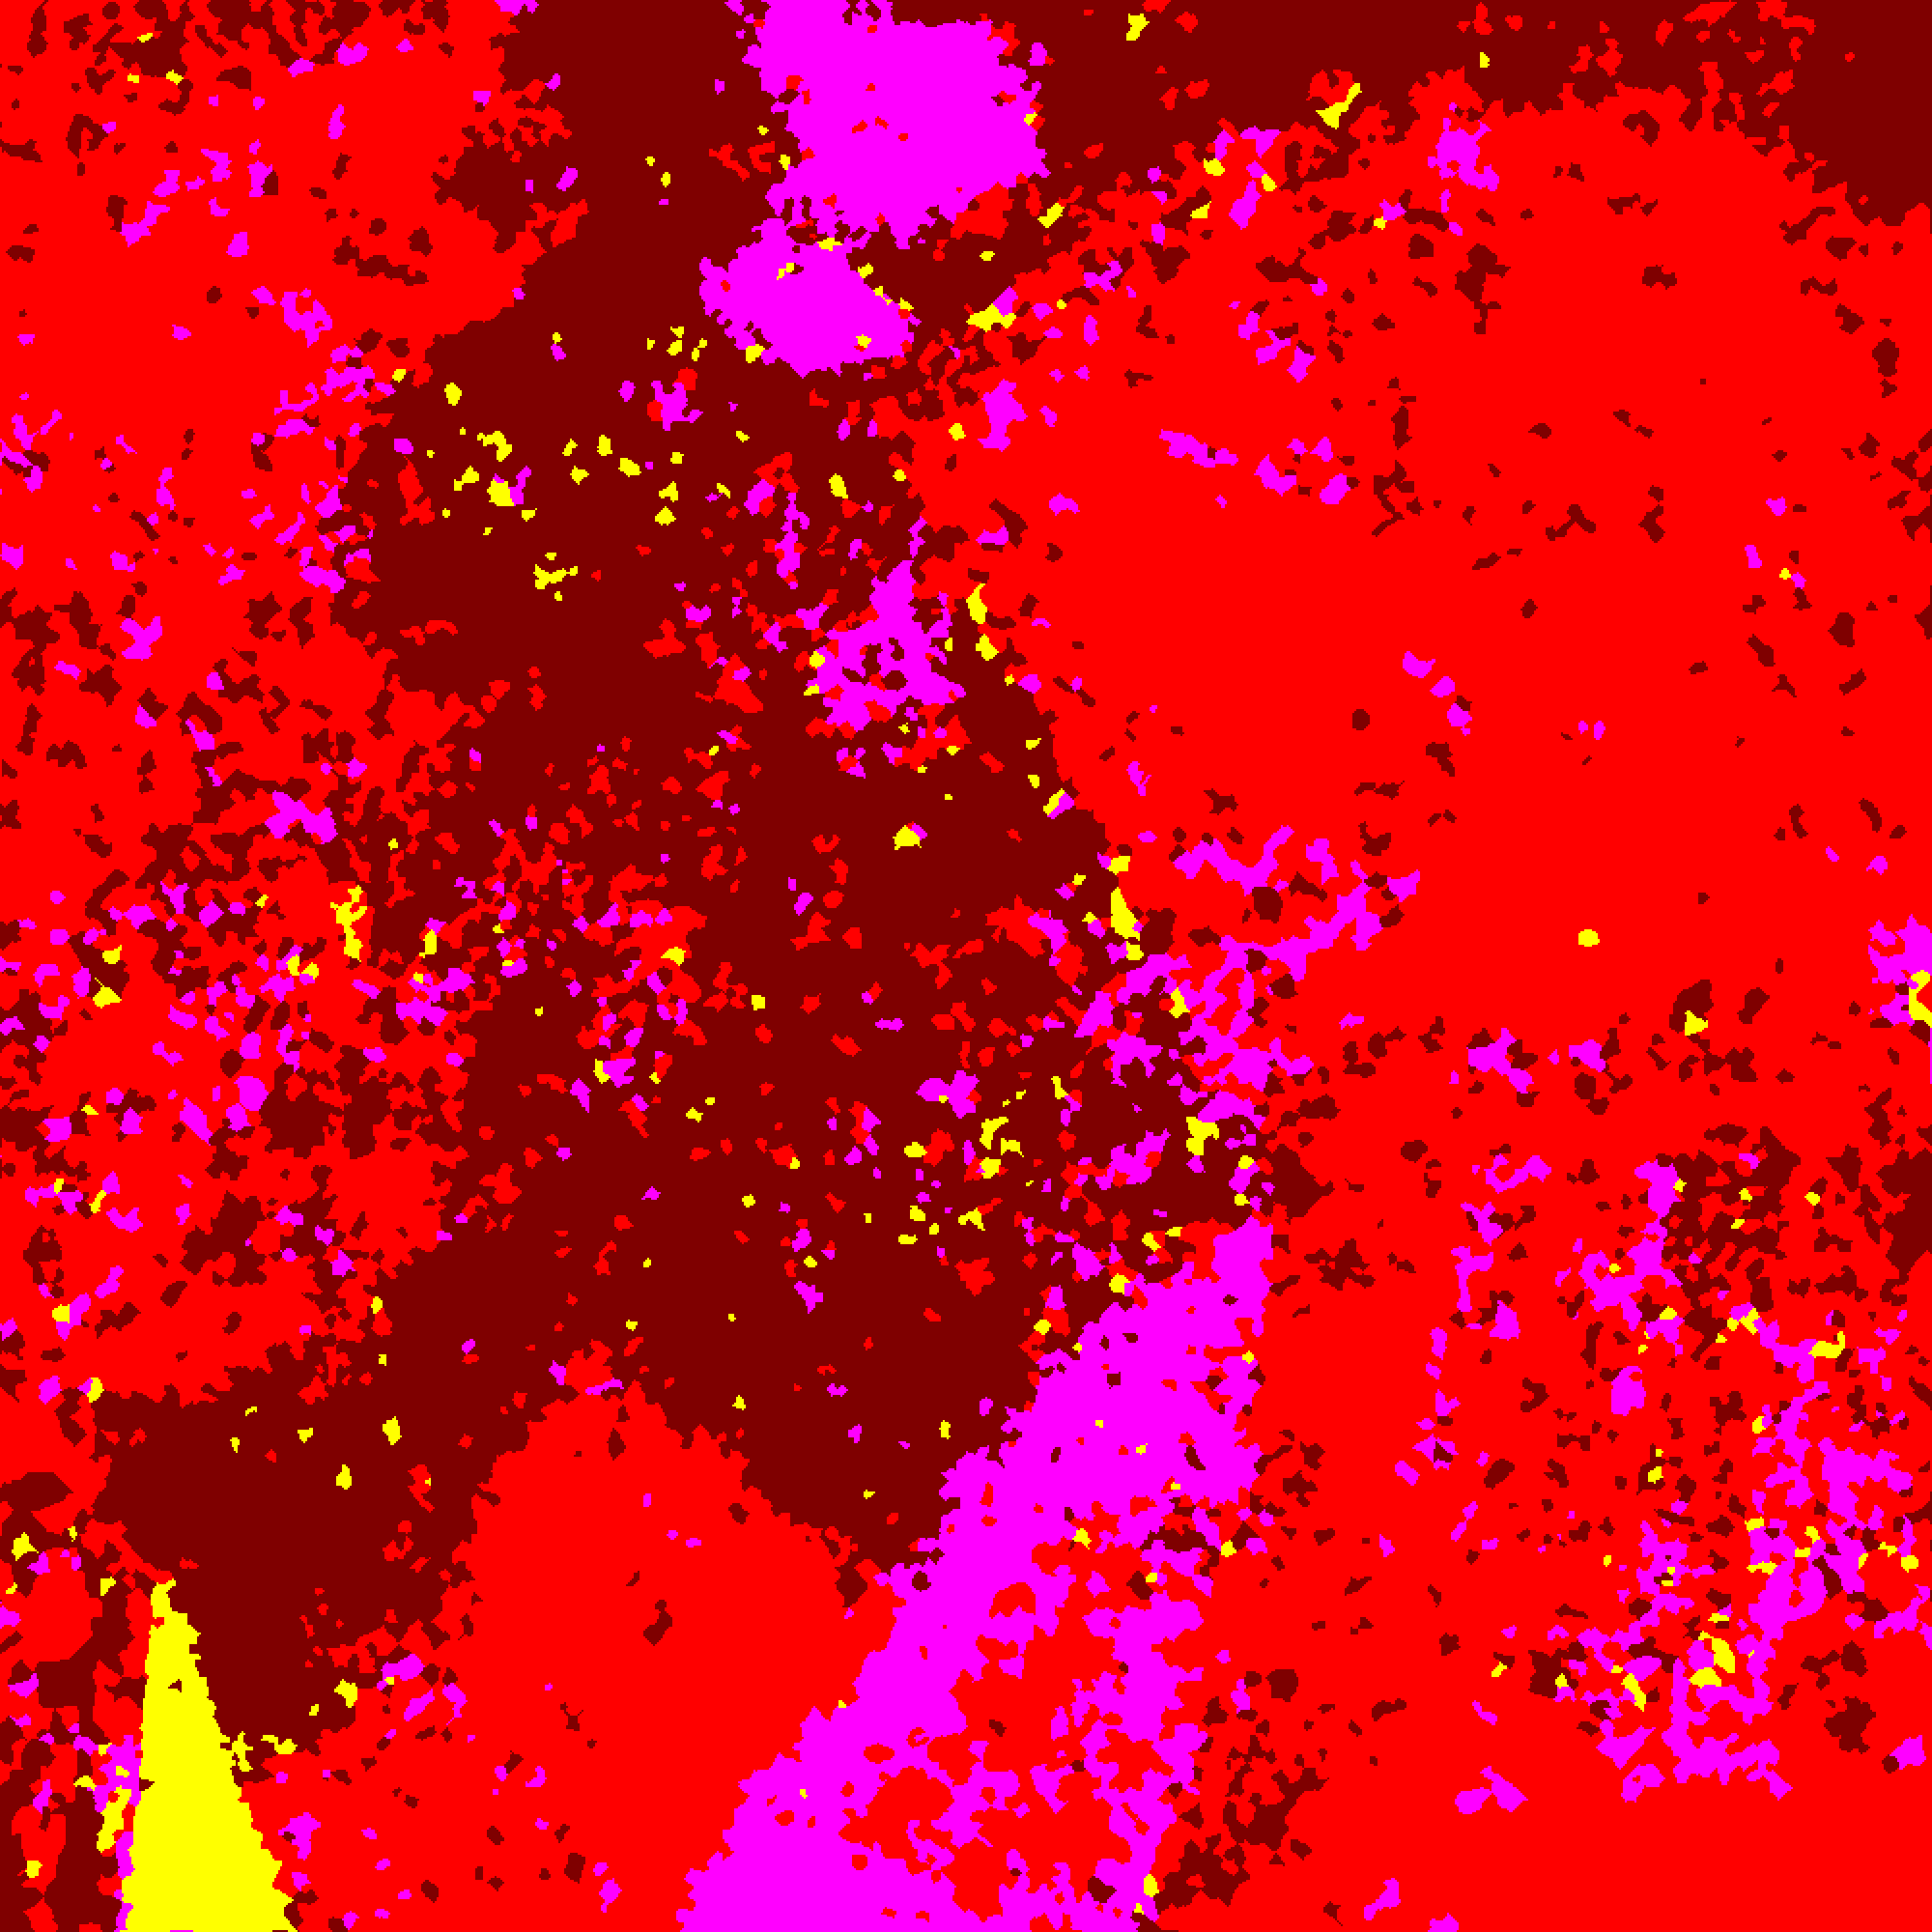
\includegraphics[width=0.45\textwidth]{Figures/C3/S2/classif}
\label{subfig:C3_S2_classifb}
}
\endgroup
\caption{Forest LC and classification results.}
\label{fig:C3_S2_classif}
\end{center}
\end{figure}

The results of the majority vote for the segmentation of the VHR optical images is presented in Figure~\ref{fig:seg_im_sem}, the confusion matrices and other metrics are presented in Tables~\ref{table:C3_S2_seg_hierar} \& \ref{table:C3_S2_seg_PFF}.

\begin{figure}[htbp]
\begin{center}
\begingroup
\captionsetup[subfigure]{width=0.3\textwidth}
\subfloat[Forest LC database.]{
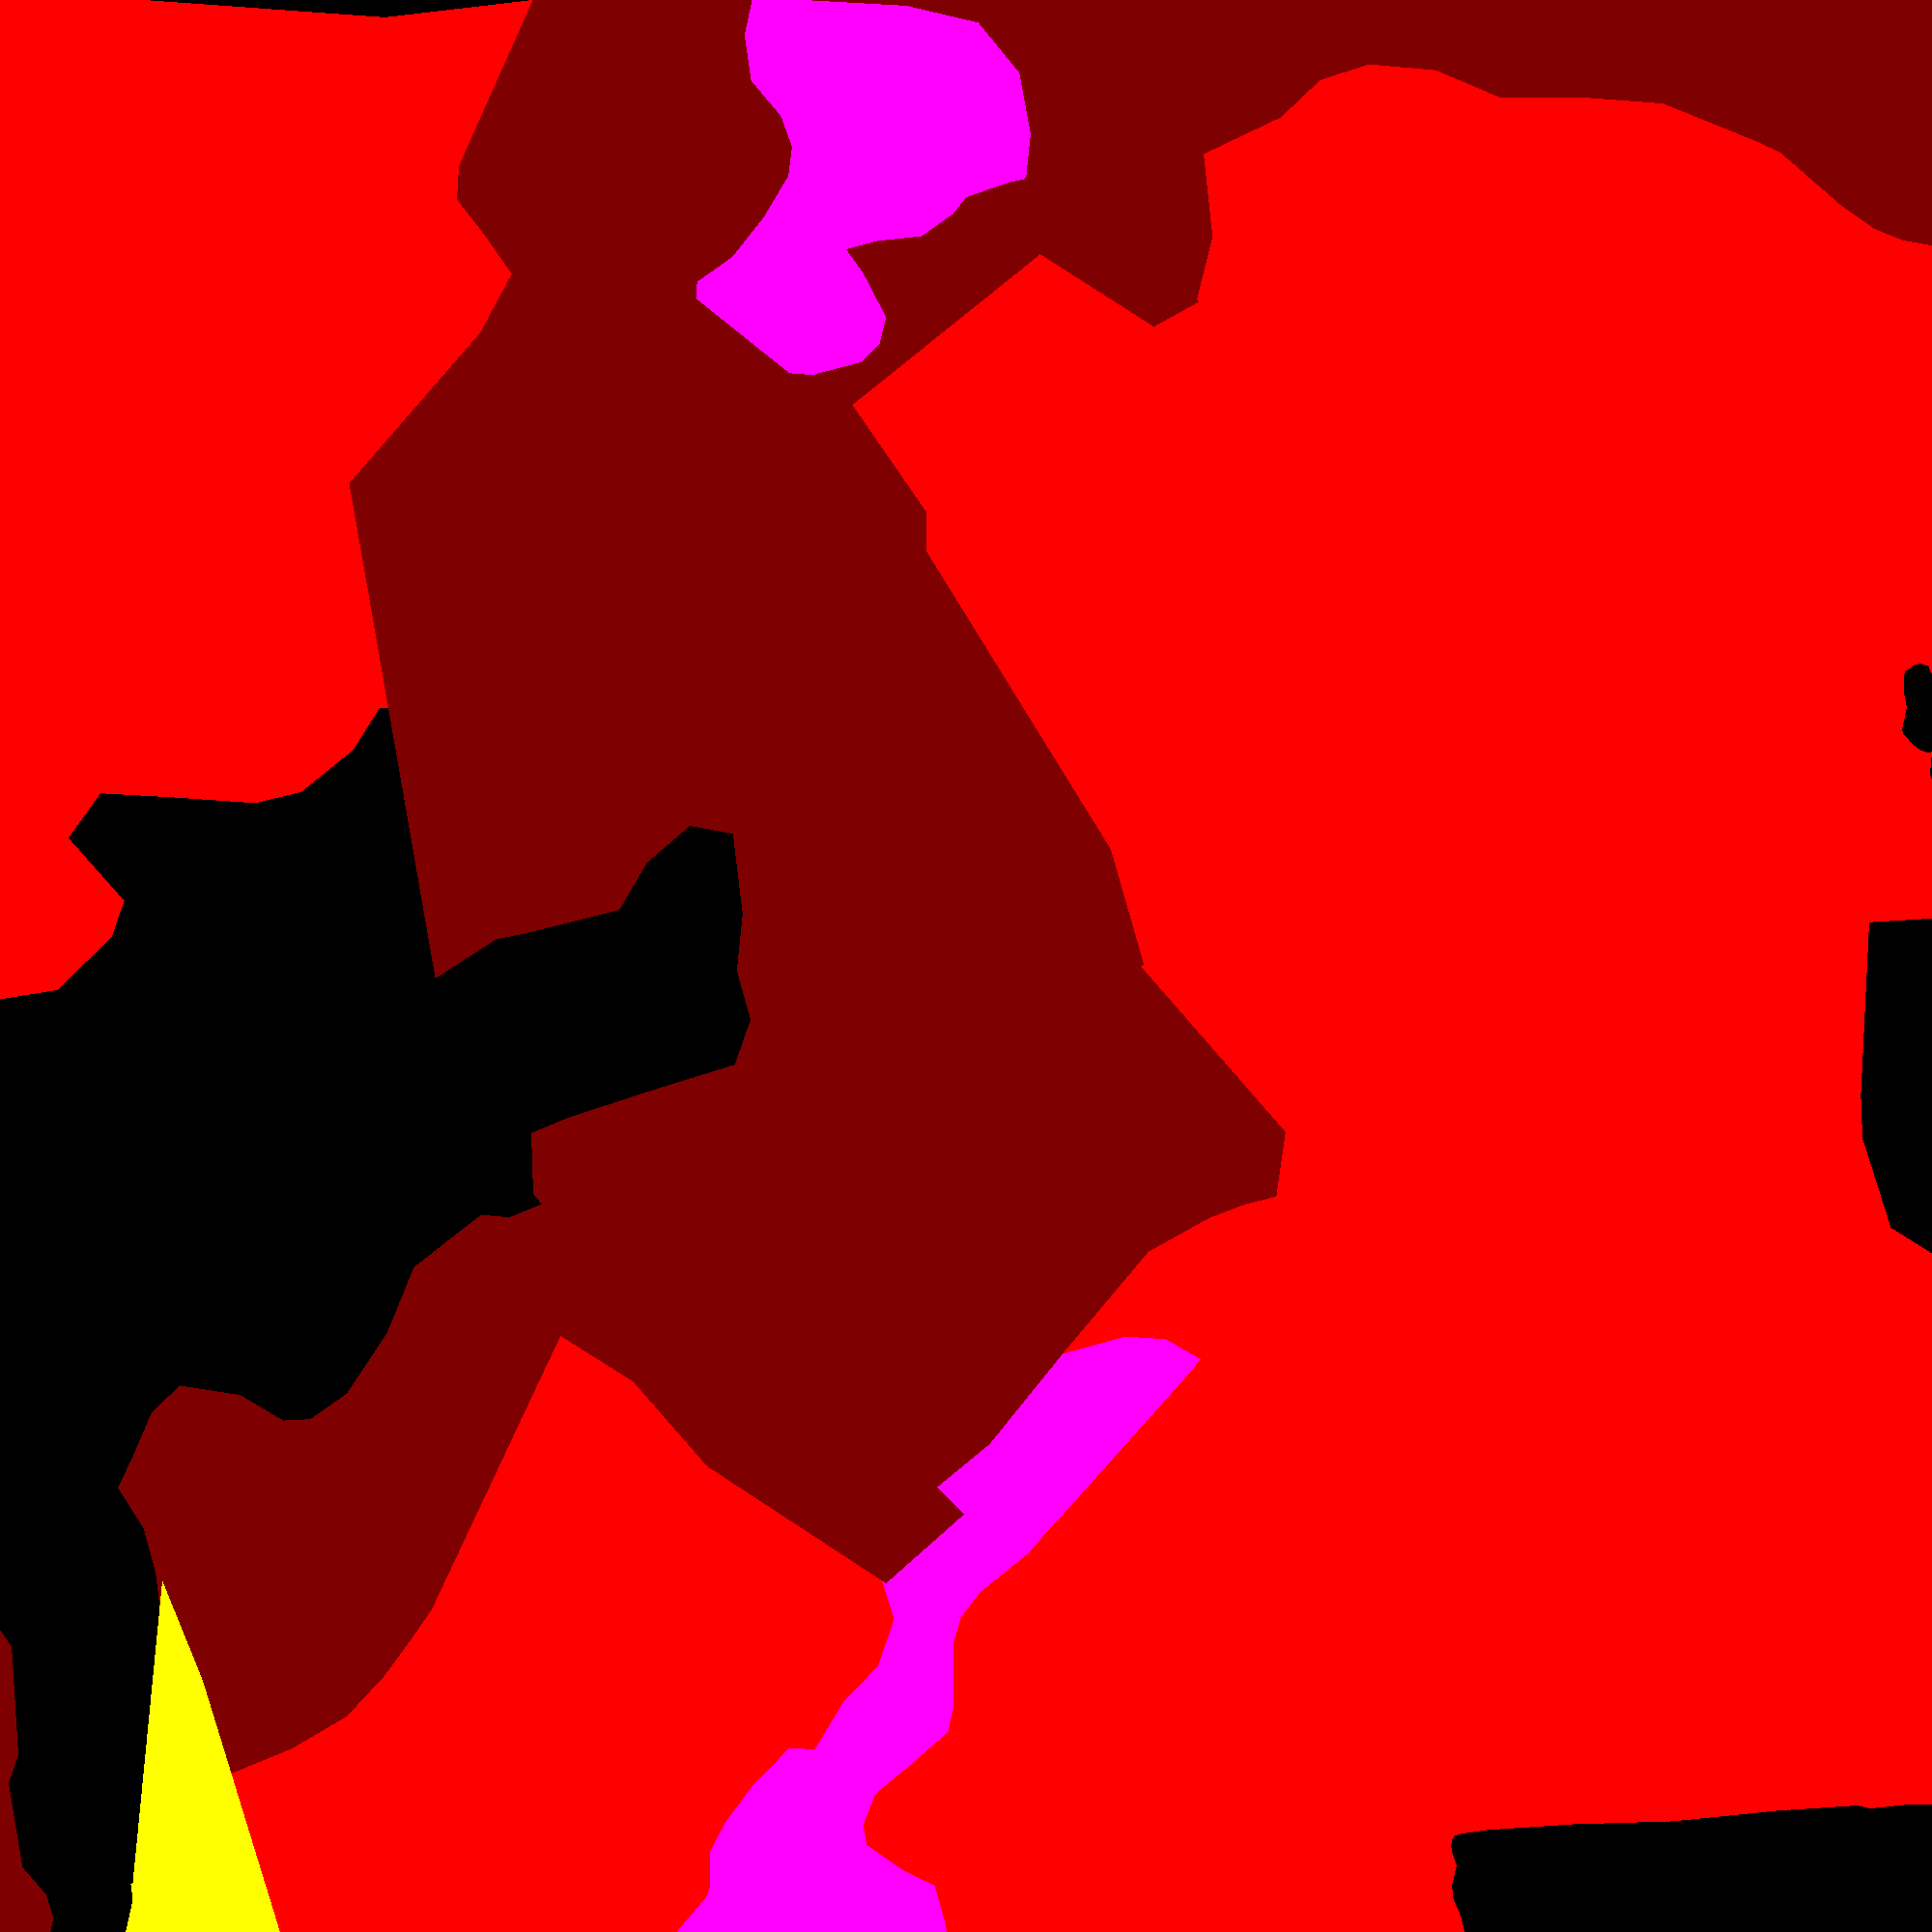
\includegraphics[width=0.3\textwidth]{Figures/C3/S2/BD}
\label{subfig:seg_im_sema}
}
\hspace*{0.025\textwidth}
\subfloat[Semantic information for the hierarchical segmentation with $\mu=15$.]{
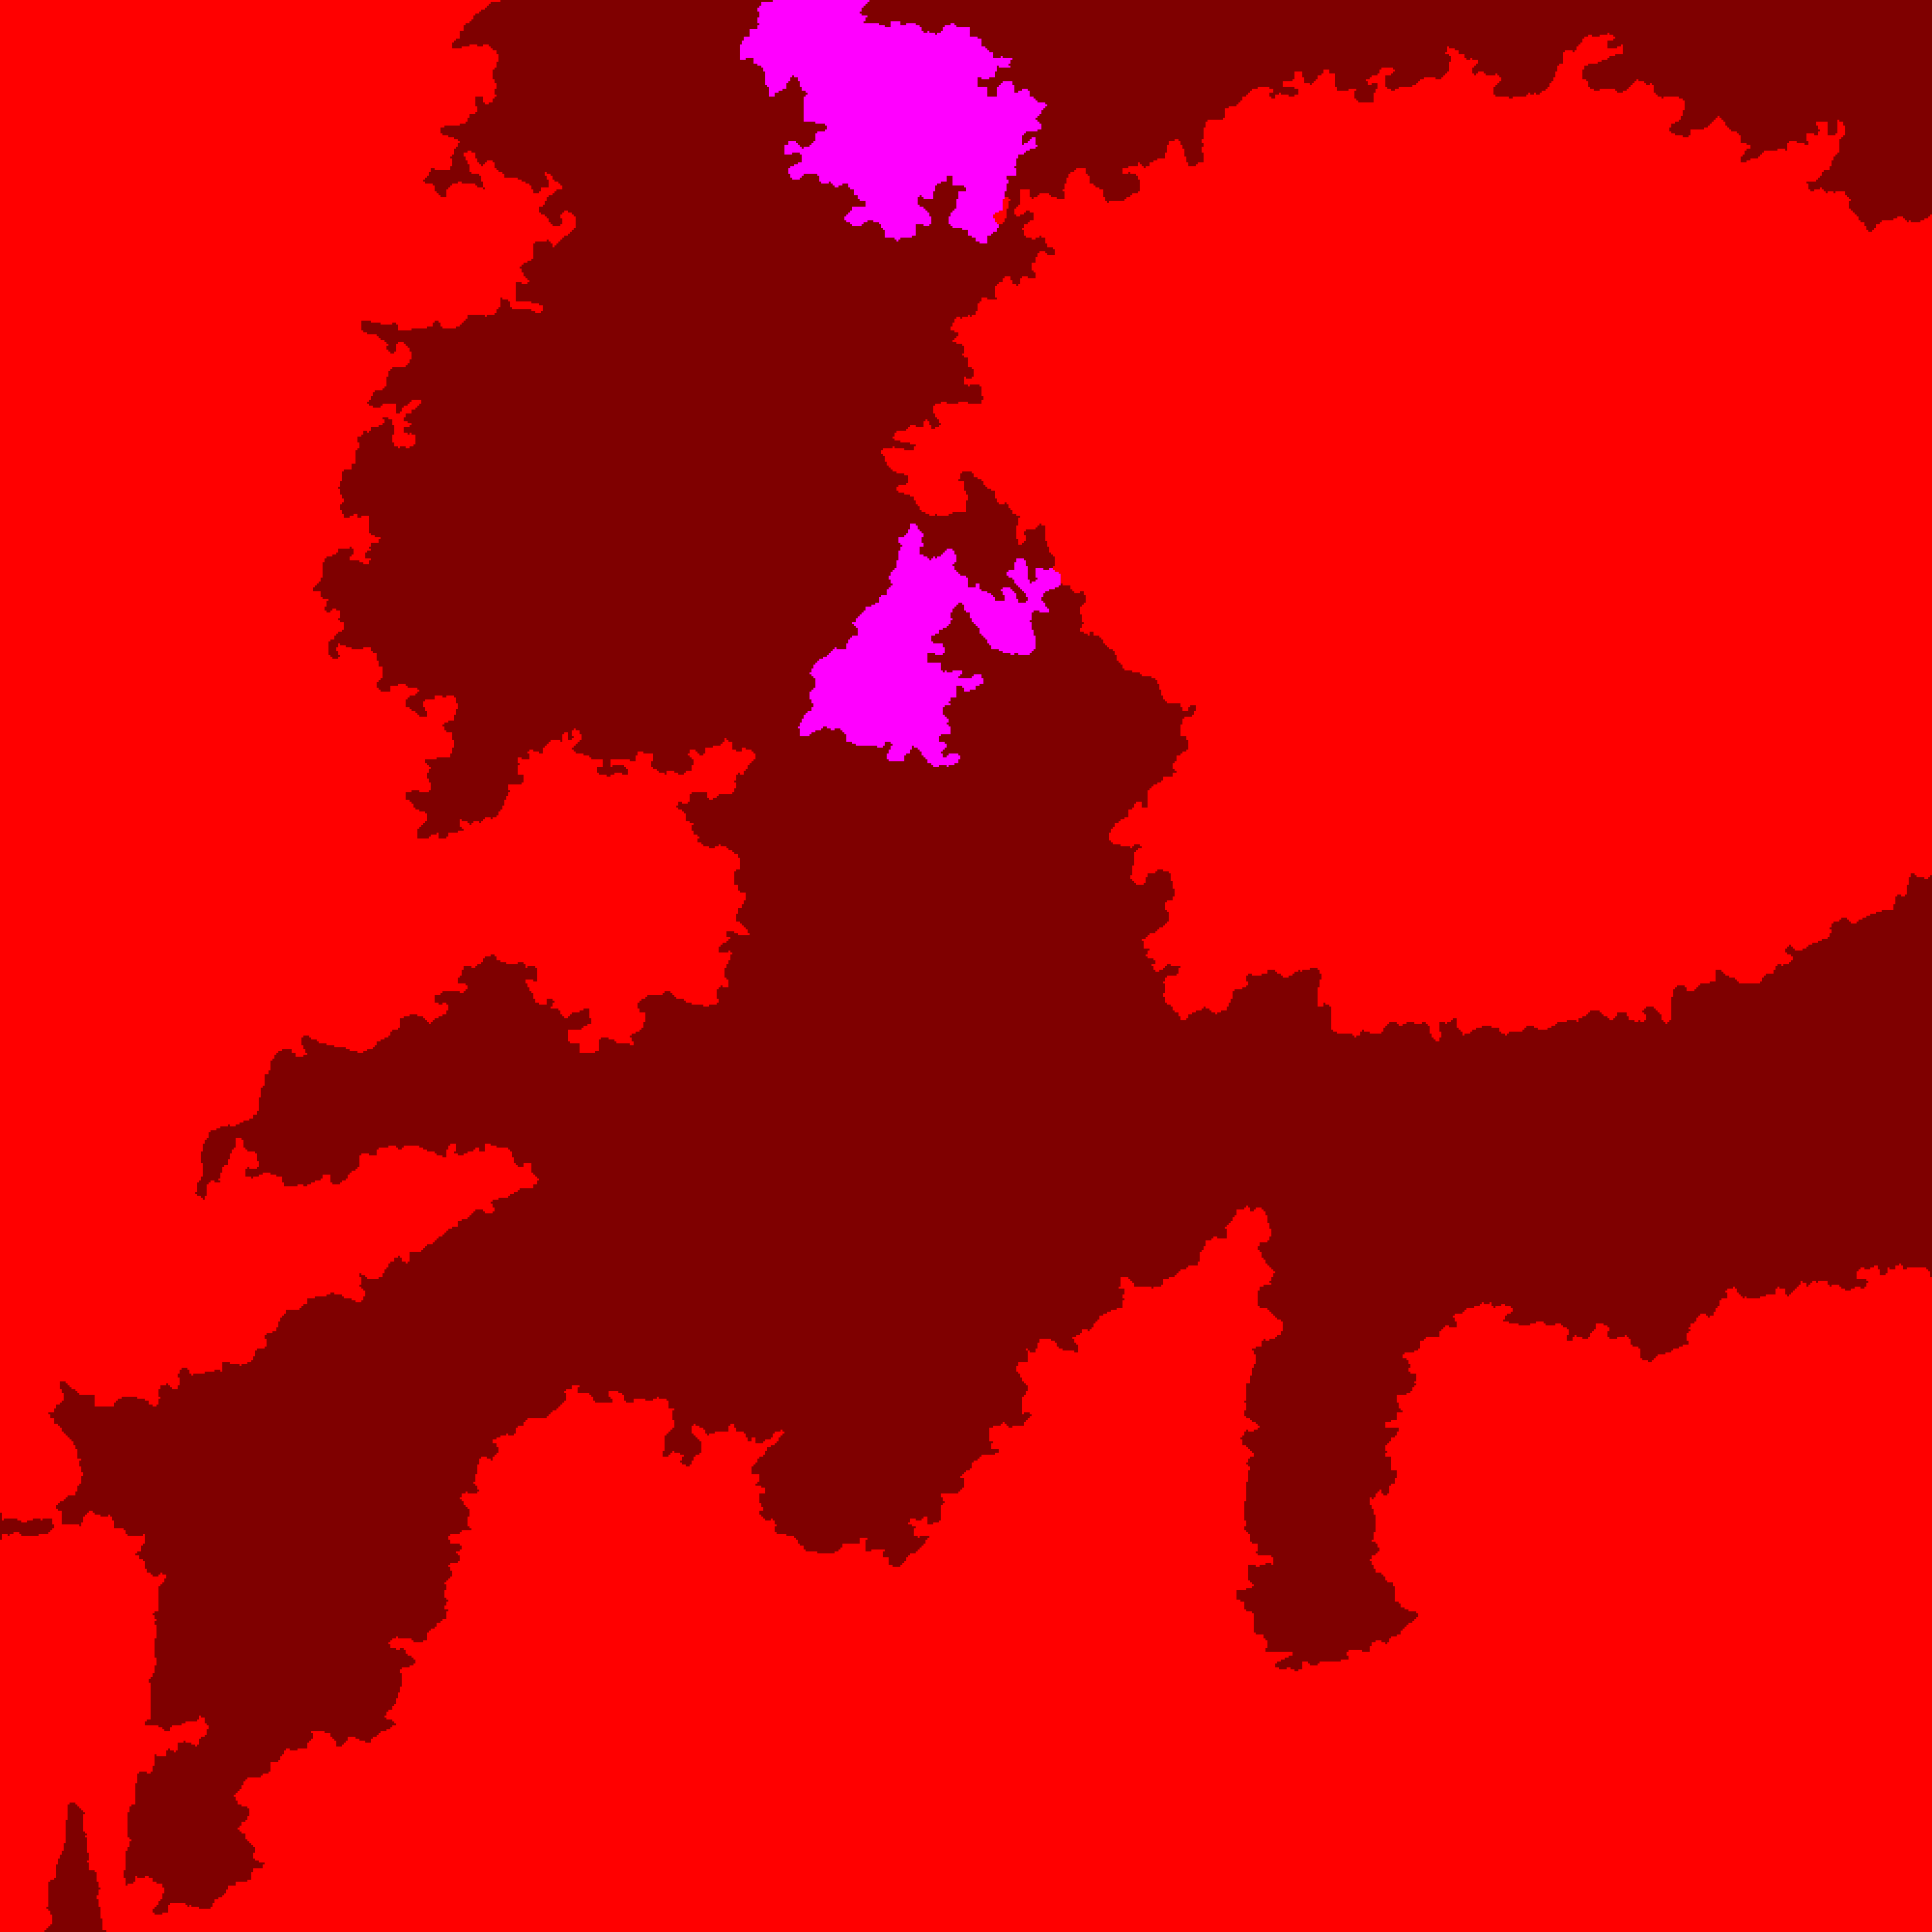
\includegraphics[width=0.3\textwidth]{Figures/C3/S2/seg_hierar_colored}
\label{subfig:seg_im_semb}
}
\hspace*{0.025\textwidth}
\subfloat[Semantic information for the PFF segmentation with $\sigma=0.8$, $k=500$ and $m=40000$.]{
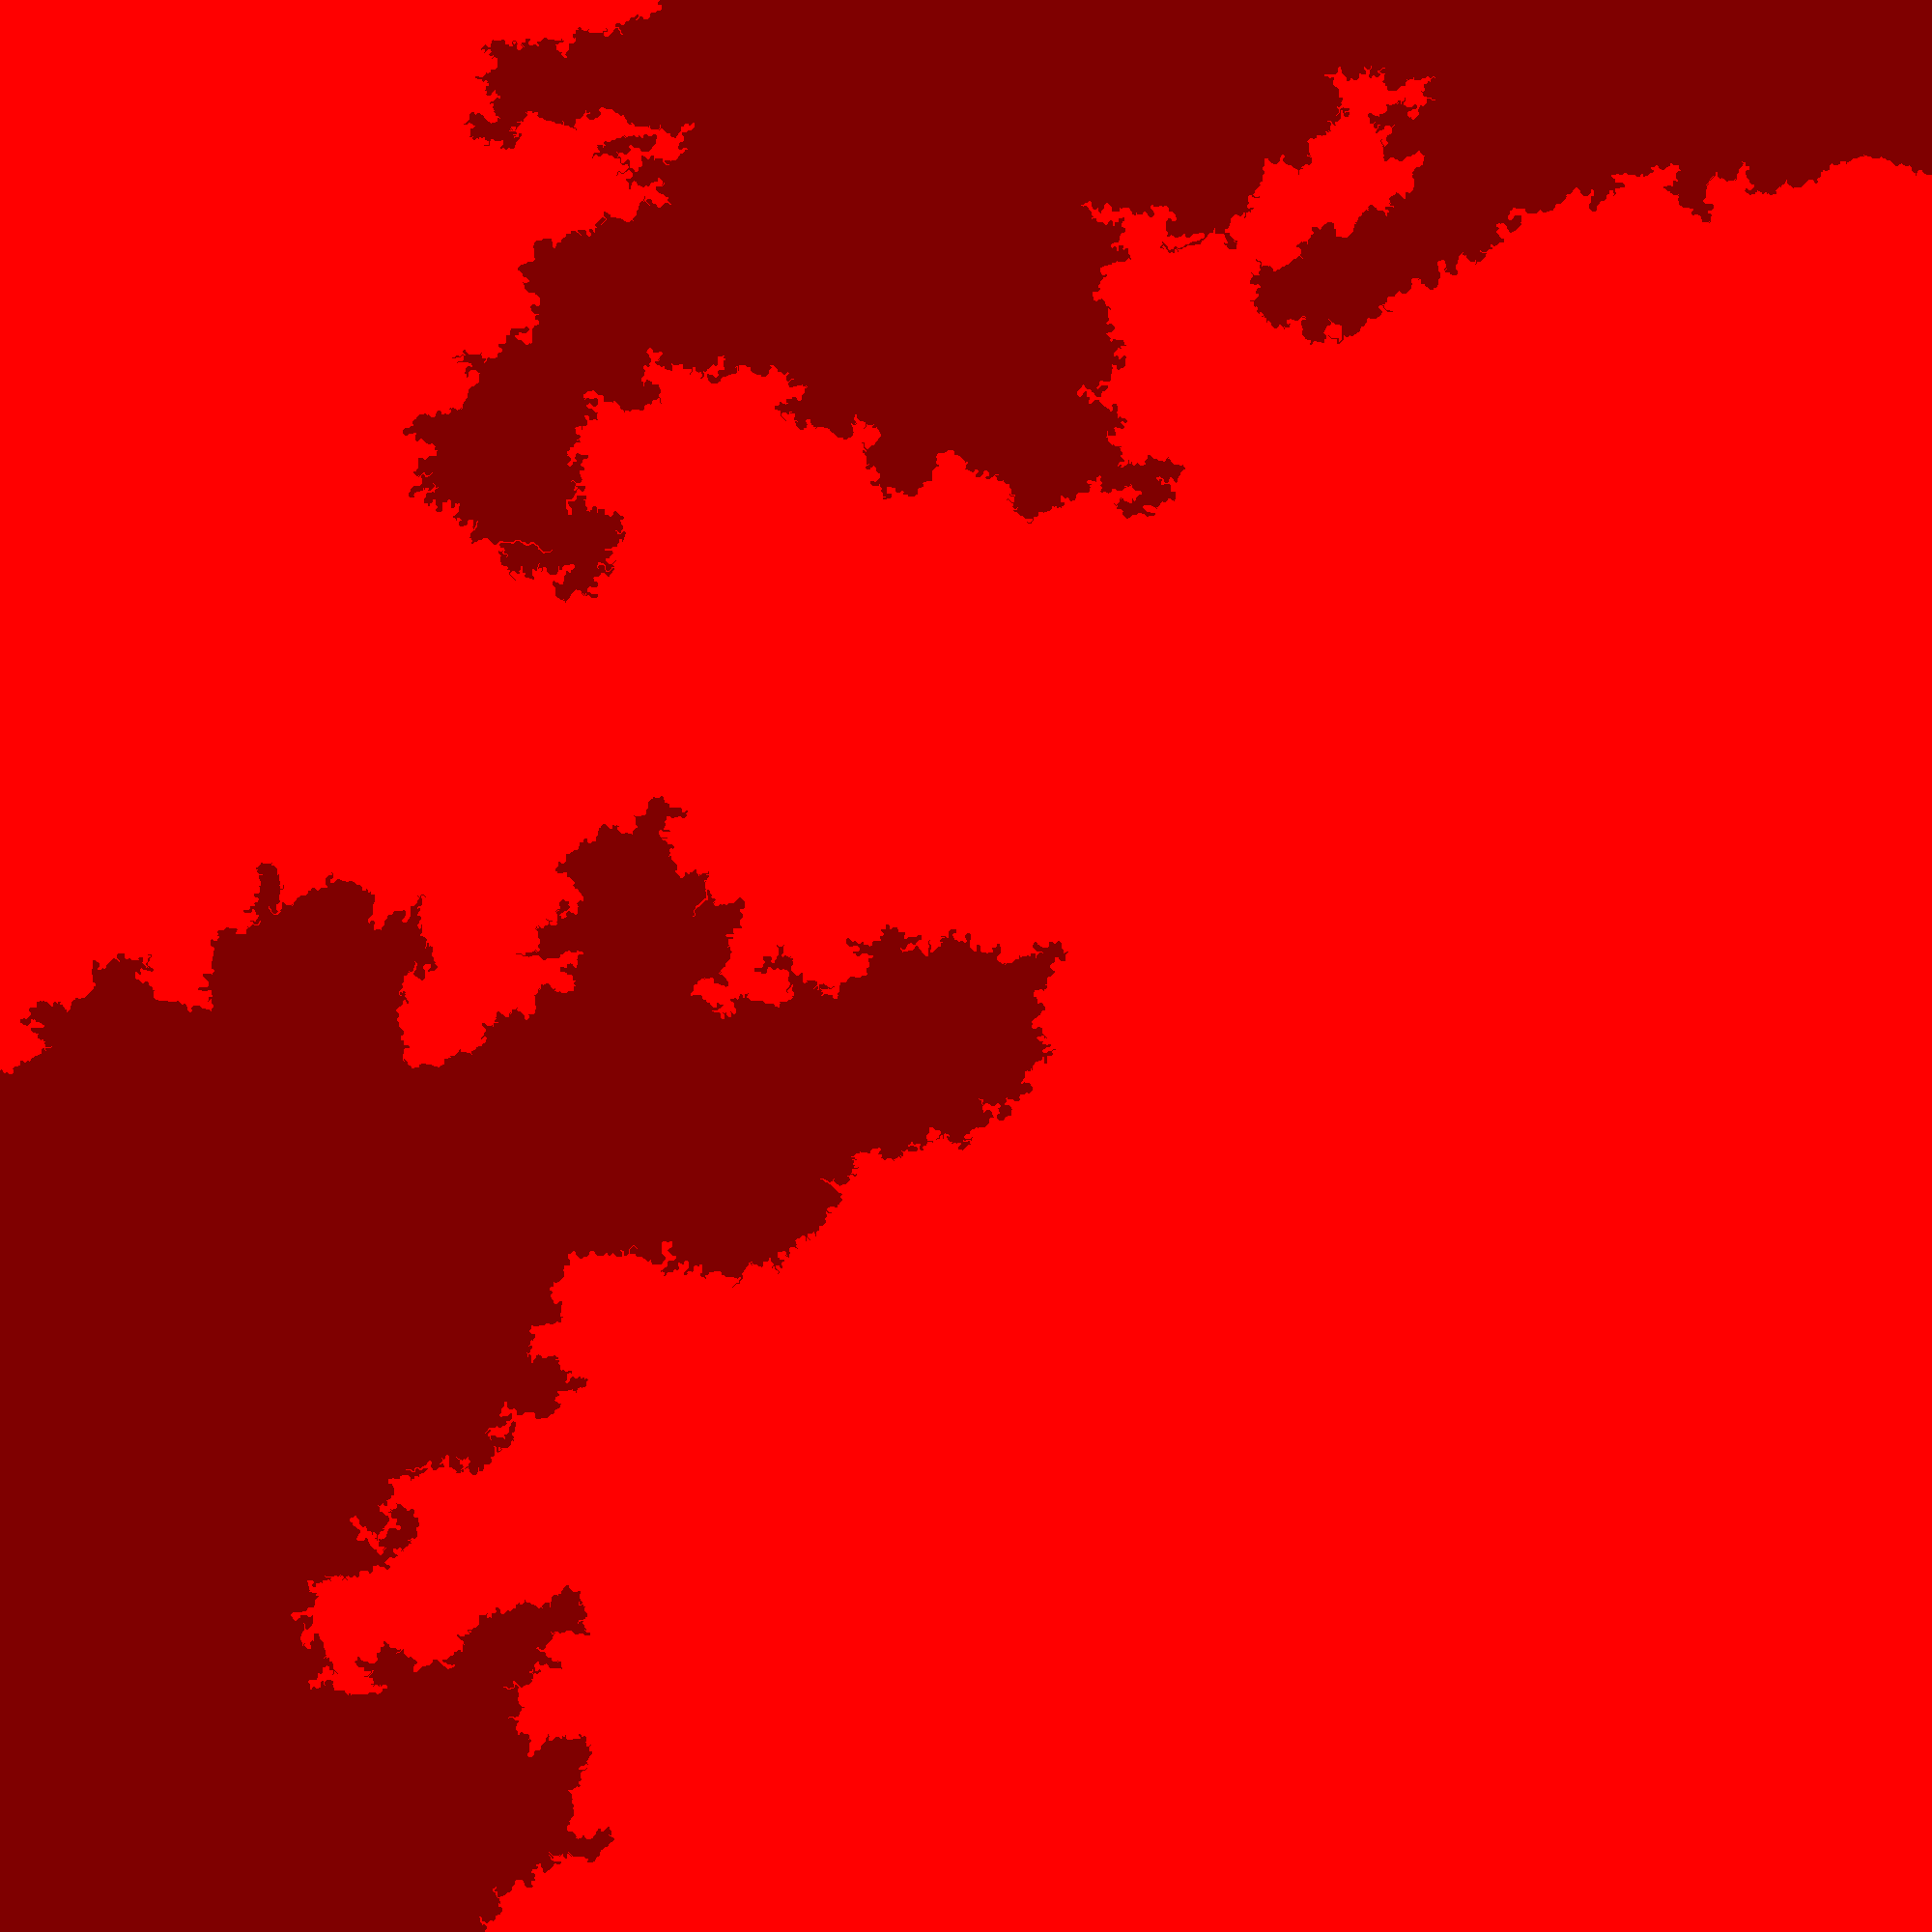
\includegraphics[width=0.3\textwidth]{Figures/C3/S2/seg_PFF_colored}
\label{subfig:seg_im_semc}
}
\endgroup
\caption{Results of the majority vote on the segmentation of the VHR optical images.}
\label{fig:seg_im_sem}
\end{center}
\end{figure}

From a visual inspection, it appears that adding semantic information to the obtained segments does not allow to retrieve a relevant mapping. Indeed, some classes are not represented. For the hierarchical segmentation, the overall accuracy increases when adding semantic information through majority vote (81.94\%, versus 81.75\% for the classification). The $\kappa$ (0.64) is also revealing a good agreement. This shows the limitation of the two metrics: the result appears to be good when inspecting them, while it is not. The Intersection over Union is more relevant in order to underline the irrelevance of the majority vote on a segmentation (41.1\%). The F-score (50.68\%) also concurs to this conclusion.

The results of the majority vote for the segmentation of the nDSM is presented in Figure~\ref{fig:seg_z_sem}, the confusion matrices and other metrics are presented in Tables~\ref{table:C3_S2_seg_hierar_z} \& \ref{table:C3_S2_seg_PFF_z}.

\begin{figure}[htbp]
\begin{center}
\begingroup
\captionsetup[subfigure]{width=0.3\textwidth}
\subfloat[Forest LC database.]{
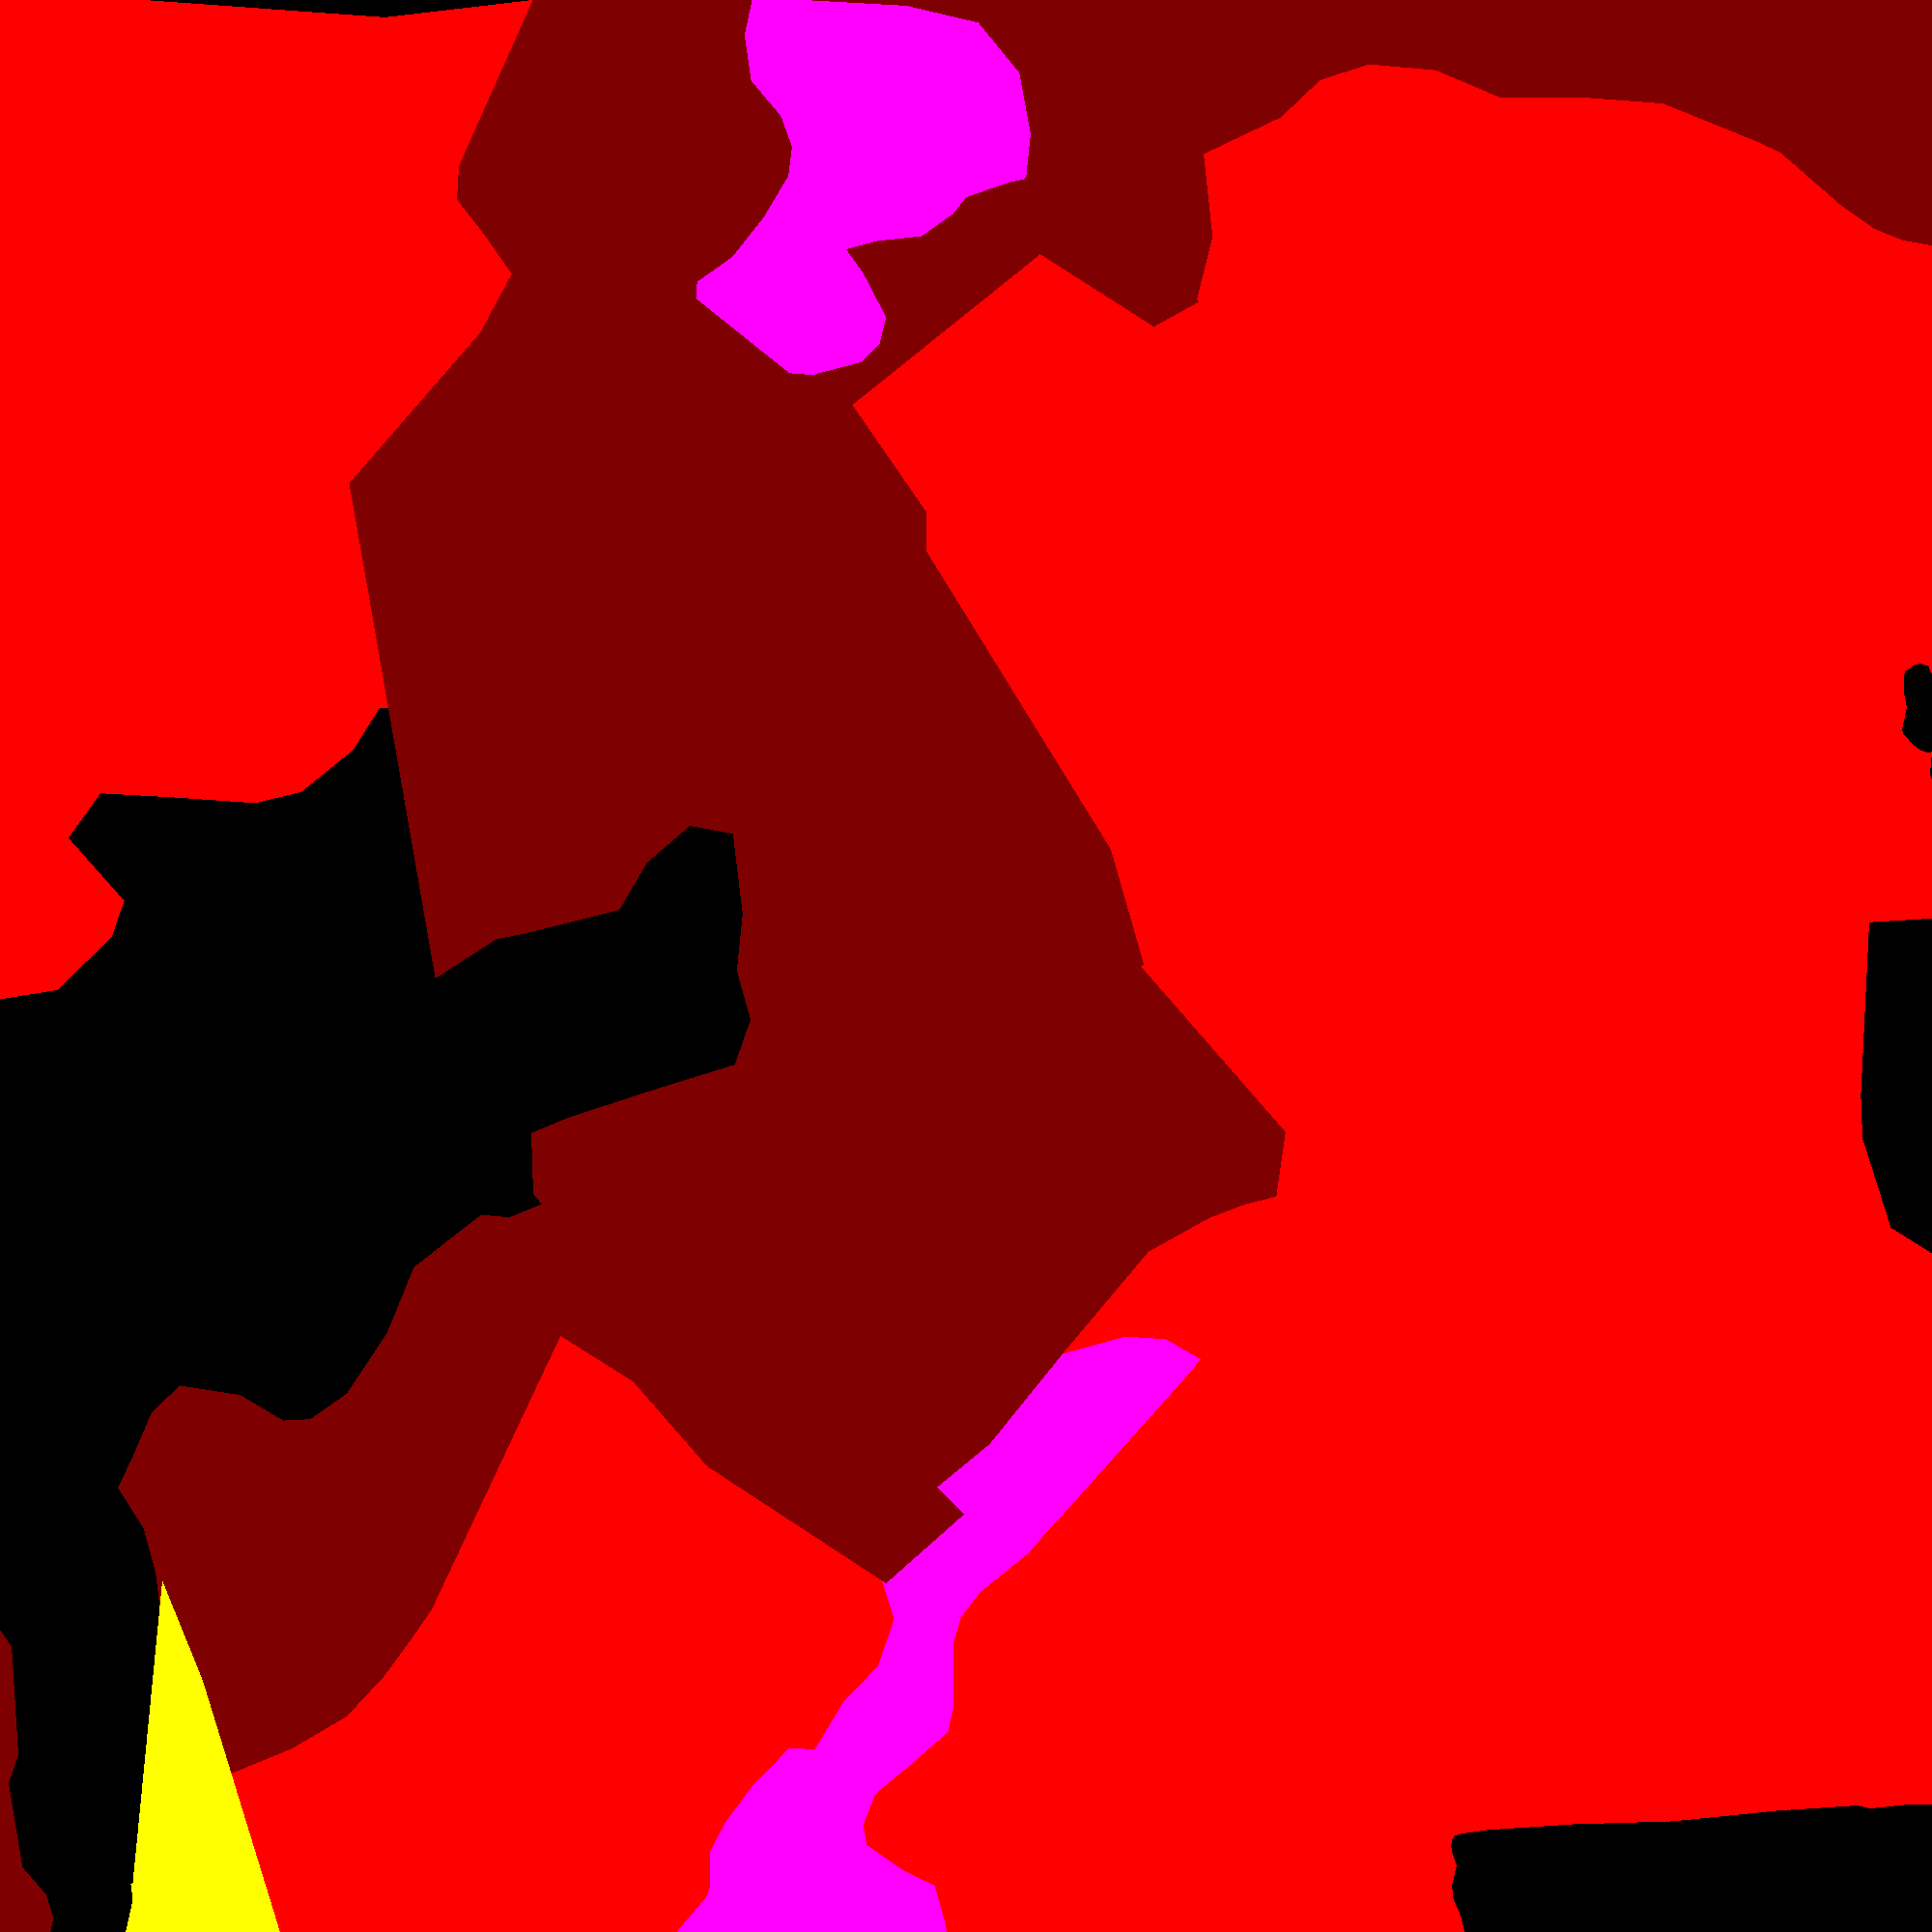
\includegraphics[width=0.3\textwidth]{Figures/C3/S2/BD}
\label{subfig:seg_z_sema}
}
\hspace*{0.025\textwidth}
\subfloat[Semantic information for the hierarchical segmentation with $\mu=15$.]{
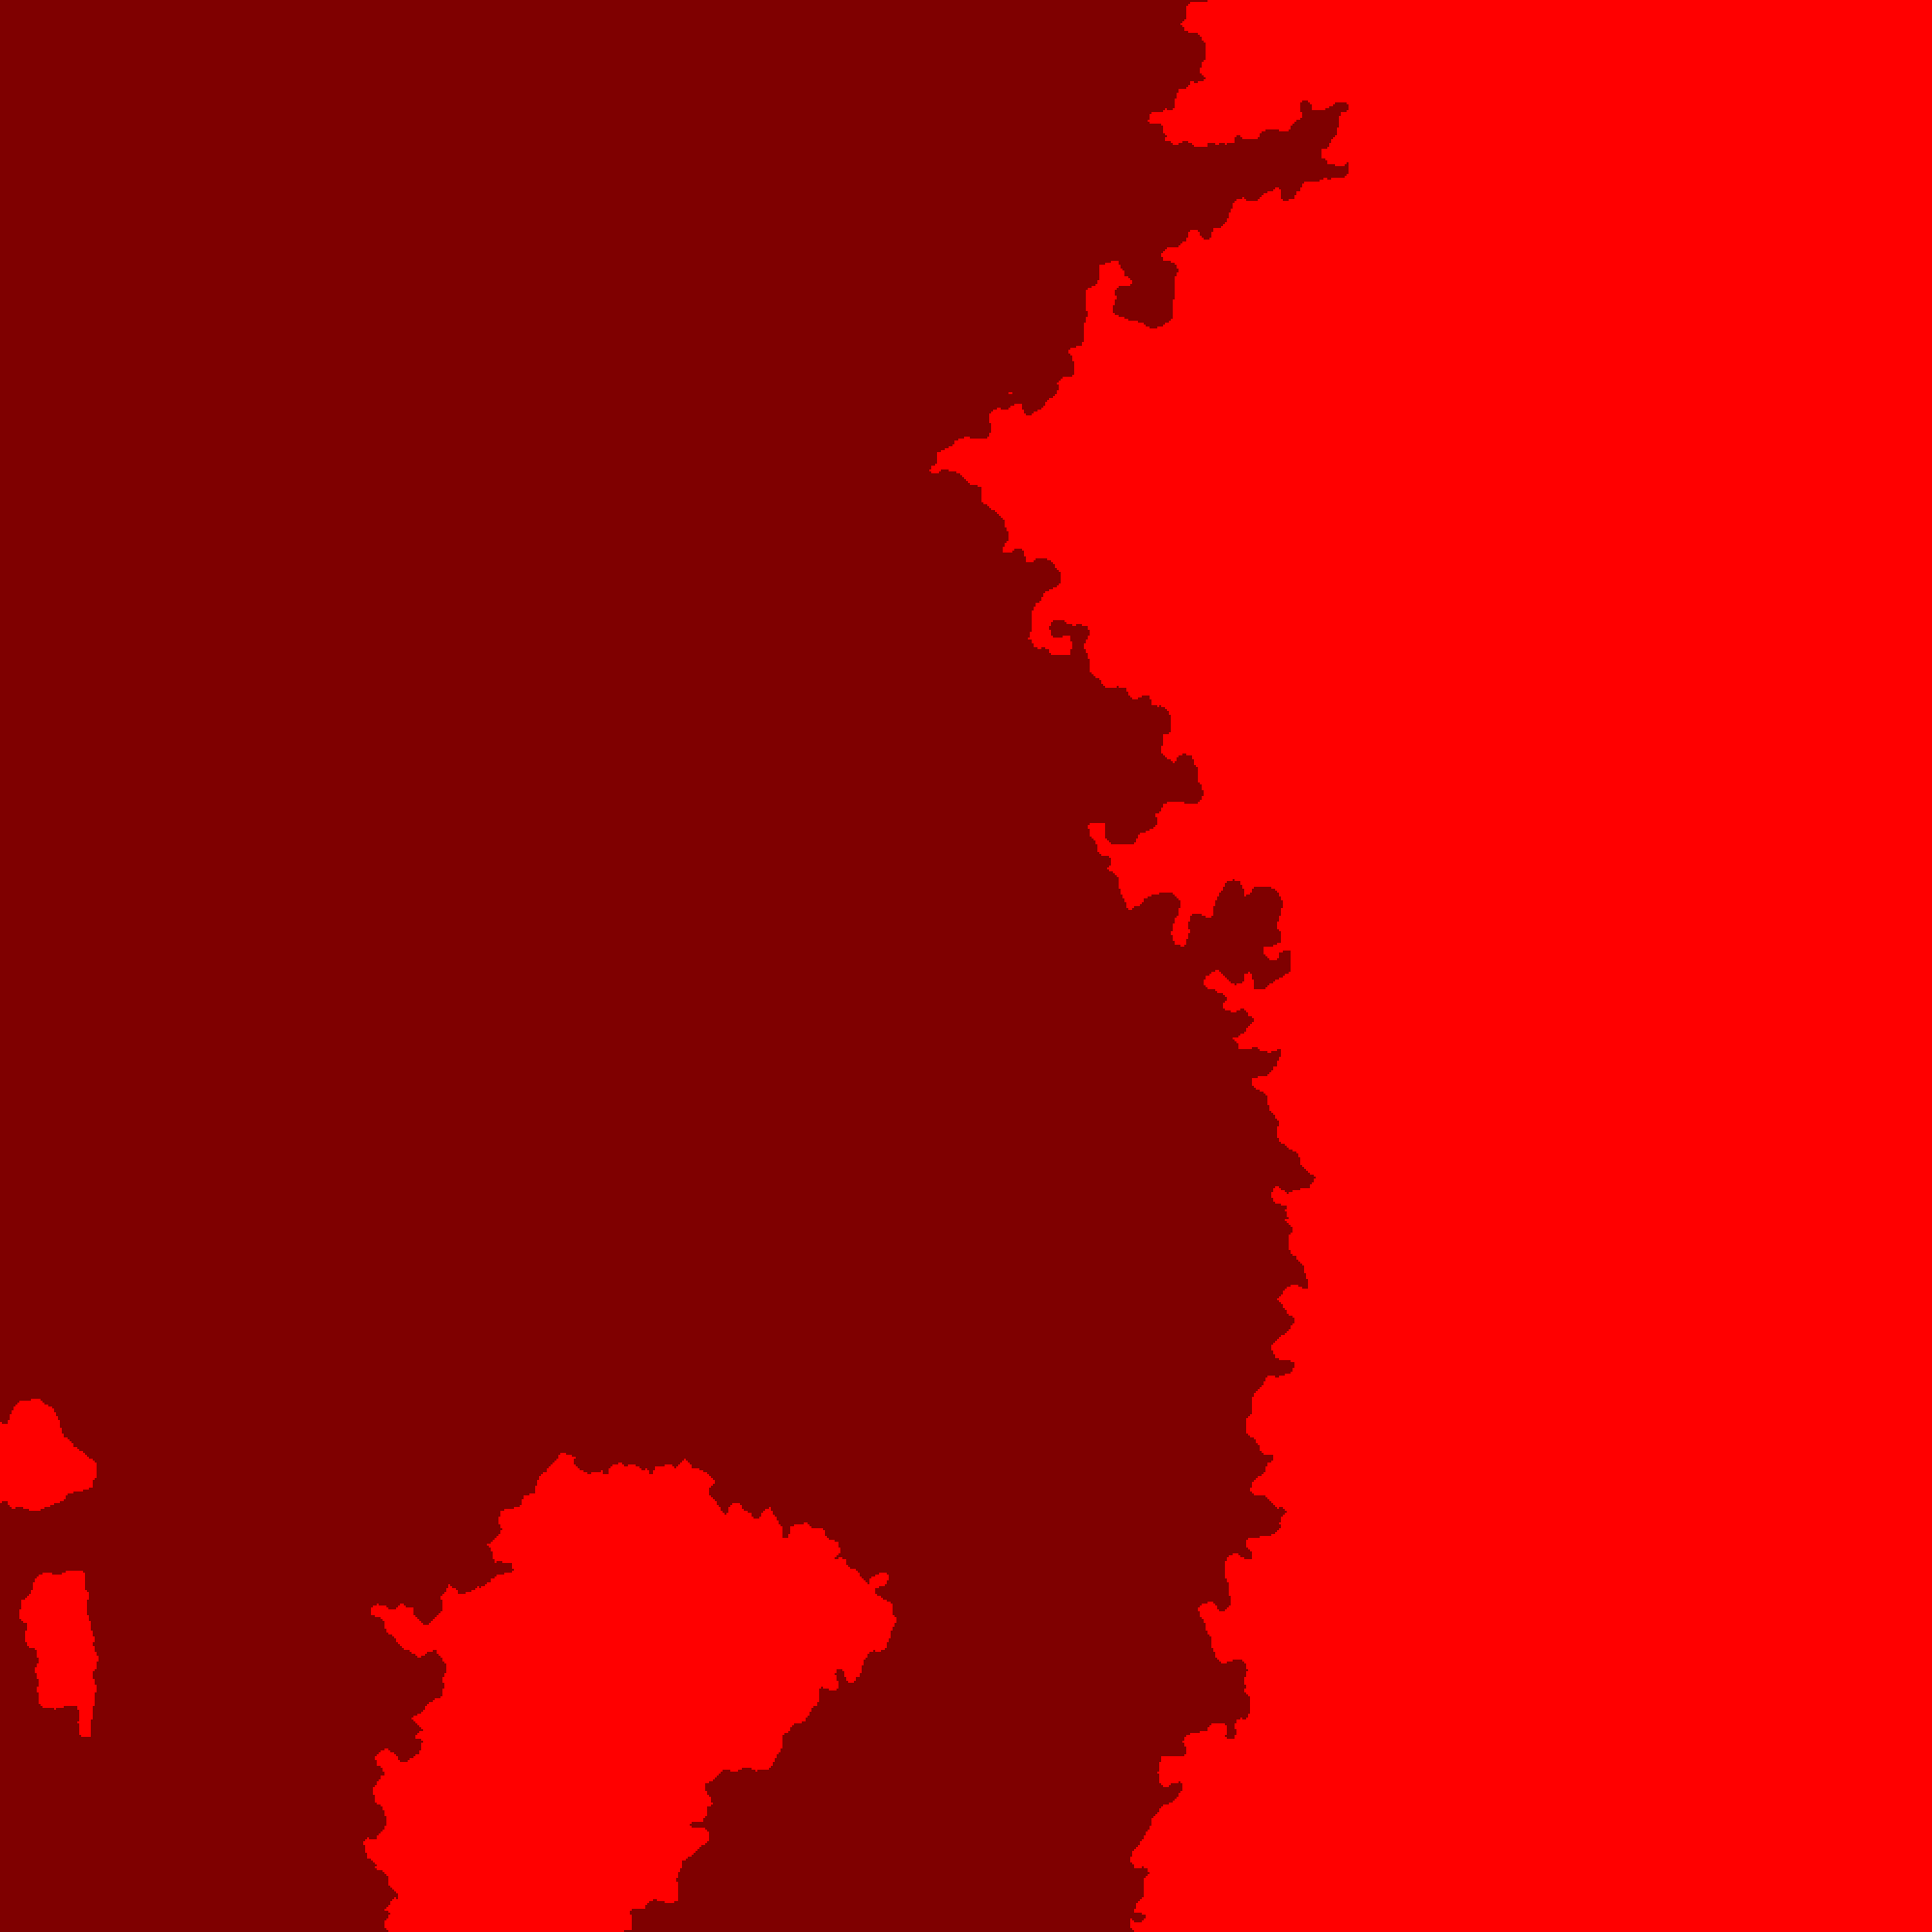
\includegraphics[width=0.3\textwidth]{Figures/C3/S2/seg_hierar_z_colored}
\label{subfig:seg_z_semb}
}
\hspace*{0.025\textwidth}
\subfloat[Semantic information for the PFF segmentation with $\sigma=0.8$, $k=500$ and $m=40000$.]{
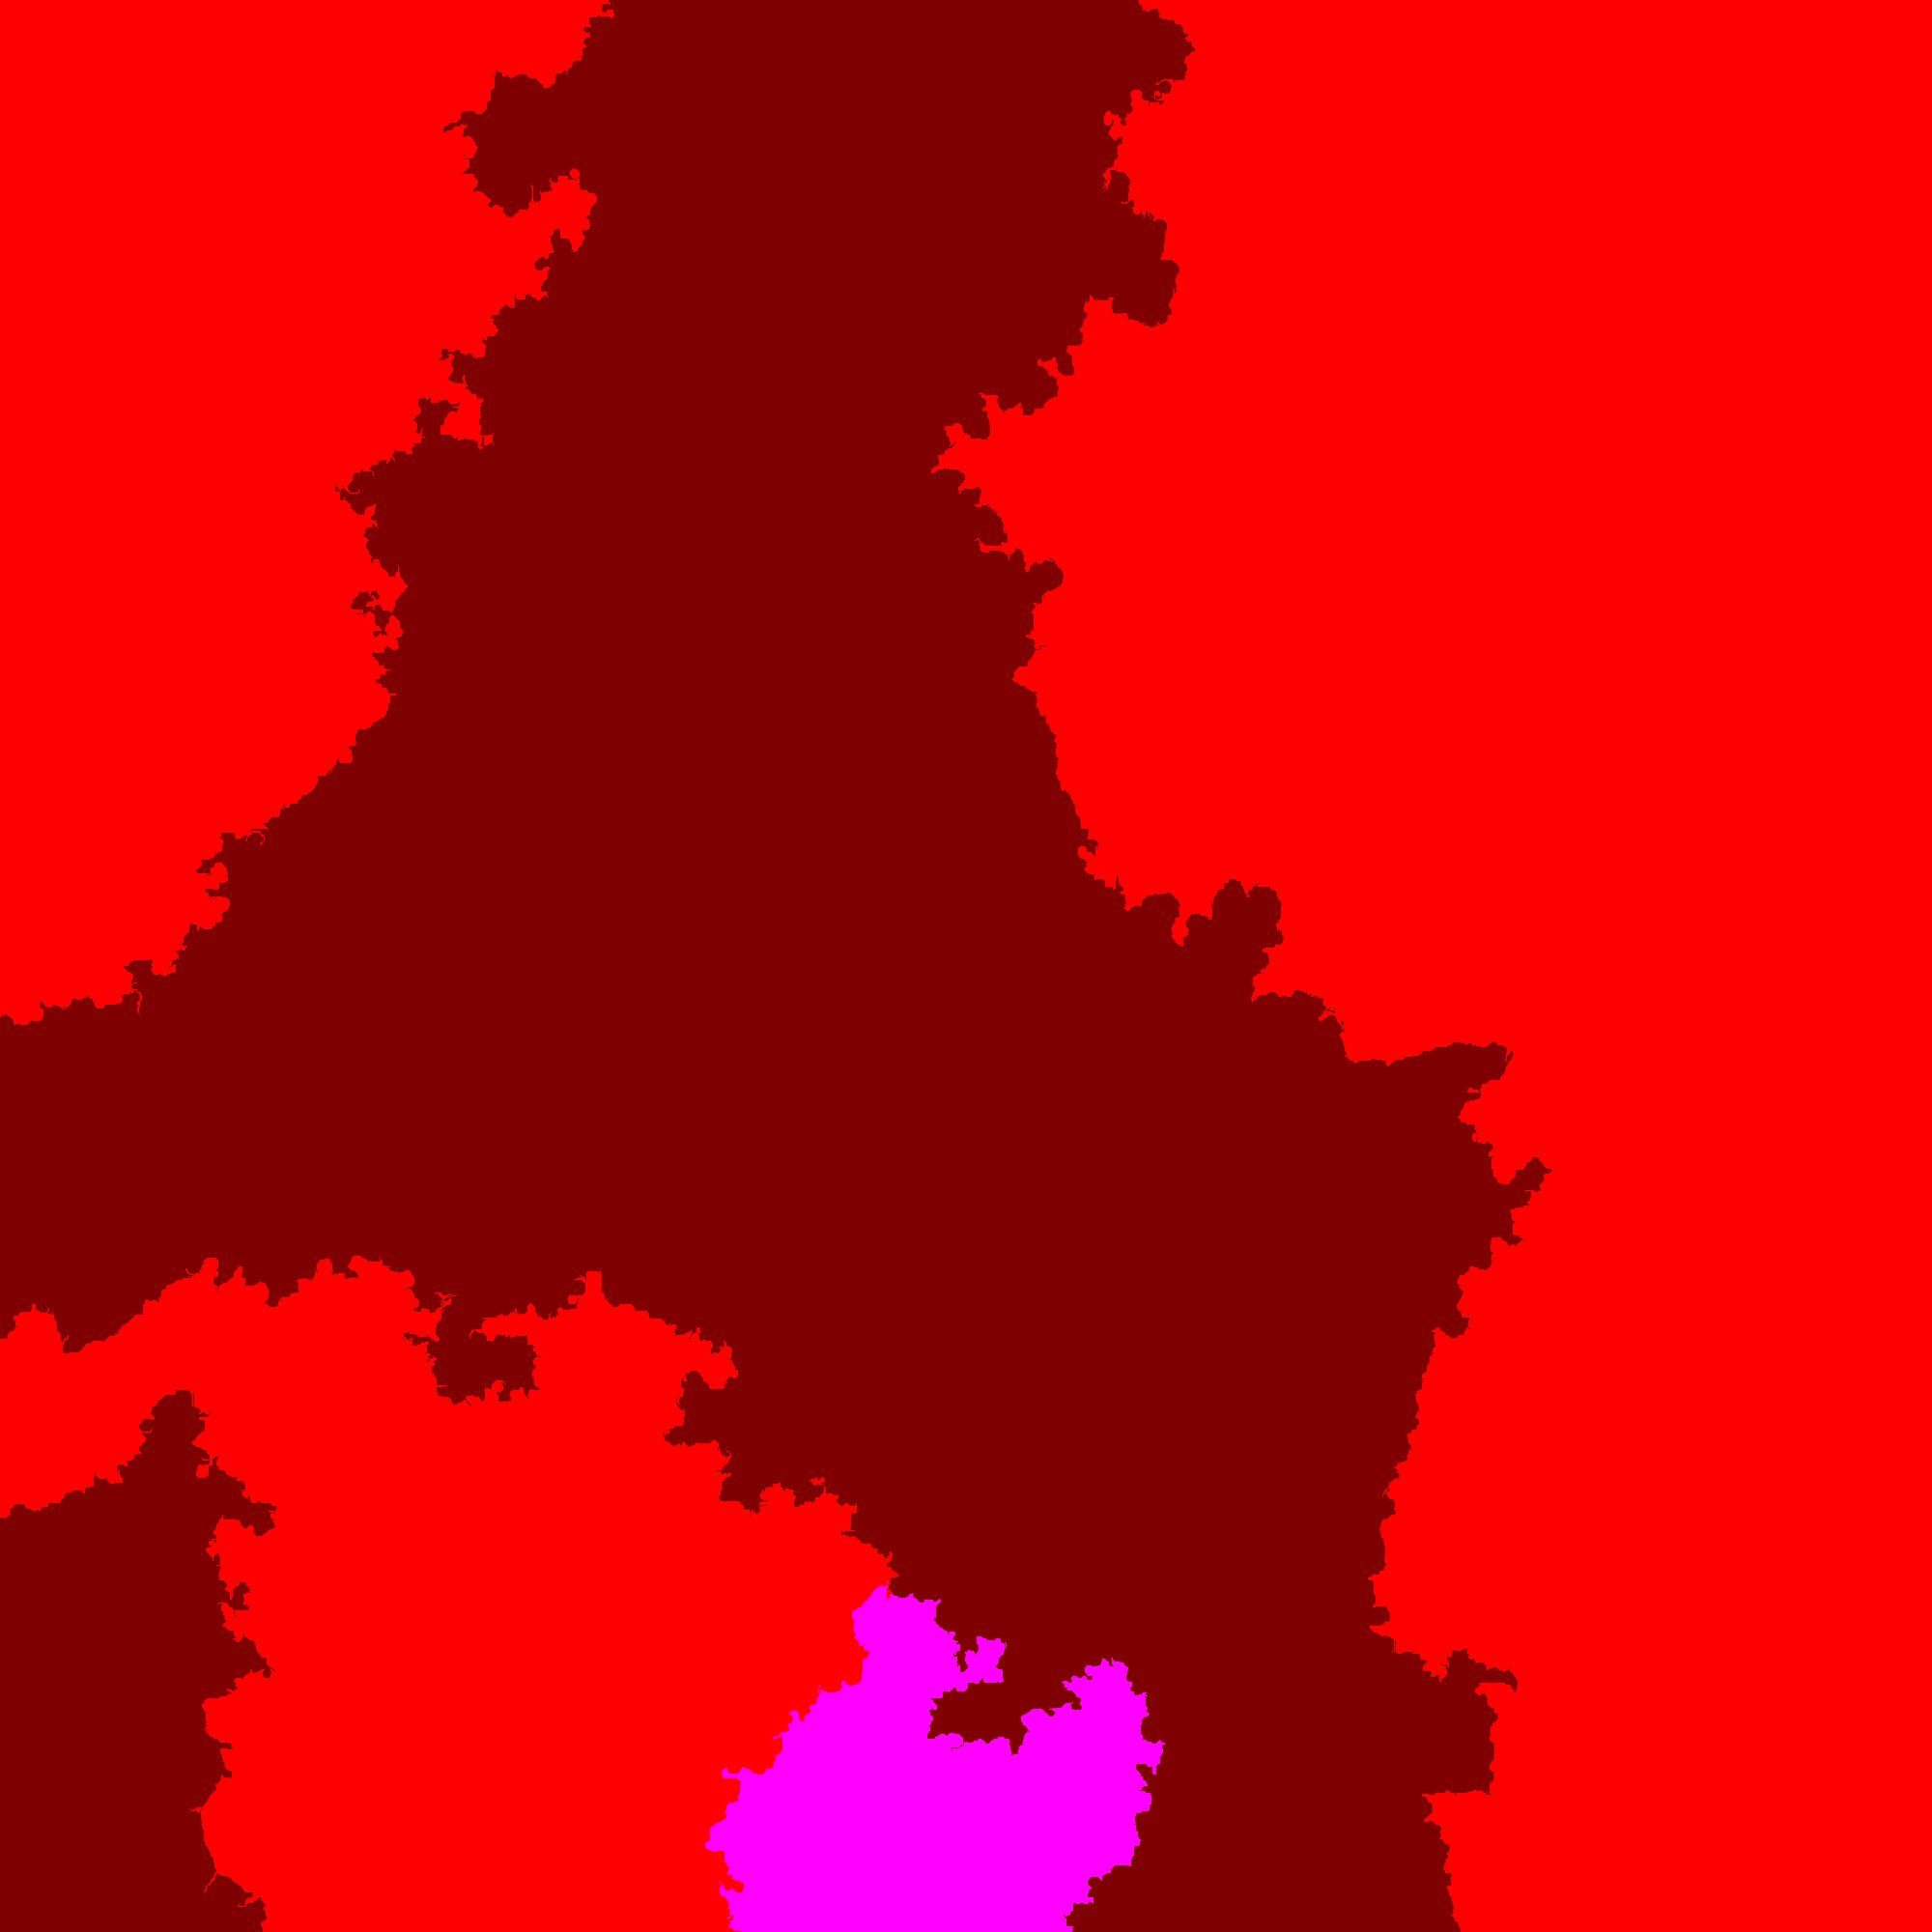
\includegraphics[width=0.3\textwidth]{Figures/C3/S2/seg_PFF_z_colored}
\label{subfig:seg_z_semc}
}
\endgroup
\caption{Results of the majority vote on the segmentation of the VHR optical images.}
\label{fig:seg_z_sem}
\end{center}
\end{figure}

The same results are observed, a majority vote applied to a segmentation equivalent to stands (in term of size) does not allow to retrieve a relevant mapping of forested areas. \\

From this section, two main conclusions can be drawn: firstly, the direct segmentation of the data does not allow to retrieve relevant forest stands in terms of species. Even with an addition of semantic information from a classification, the results are not sufficient for a mapping of the forest. Secondly, some metrics are not relevant in order to evaluate the results. Indeed, the overall accuracy or the $\kappa$ are not sufficient, other metrics are needed for the correct evaluation of the results.

\section{Results of the method}
The proposed method is composed of different steps (defined above). Each step will be evaluated at 2 levels; the direct output will be first considered and the impact on the final segmentation will also be investigated. In order to simplify the reading of captions, when no specific information is provided the method is employed using the following parameters:
\begin{itemize}
\item Feature selection:
\begin{itemize}
\item Selection of training samples,
\item Selection of 20 features,
\item Object-based features (lidar and spectral) obtained from the PFF over-segmentation,
\item Pixel-based features (lidar and spectral) for the regularization.
\end{itemize}
\item Classification performed with:
\begin{itemize}
\item Selection of training samples,
\item Object-based features (lidar and spectral) obtained from the feature selection.
\end{itemize}
\item Regularization using global method with:
\begin{itemize}
\item $\gamma=10$,
\item Linear data formulation,
\item \textit{Exponential-features model} with pixel-based features obtained from the feature selection.
\end{itemize}
\end{itemize}
\subsection{Over-segmentation}
\label{sec:C3_S3_ss1}
The results of the over-segmentation of proposed segmentation algorithms are presented in Figure~\ref{fig:C3_S3_ss1_seg}.

\begin{figure}[htbp]
\begin{center}
\begingroup
\captionsetup[subfigure]{width=0.325\textwidth}
\subfloat[RGB VHR optical image (250$\:$m$\times$250$\:$m).]{
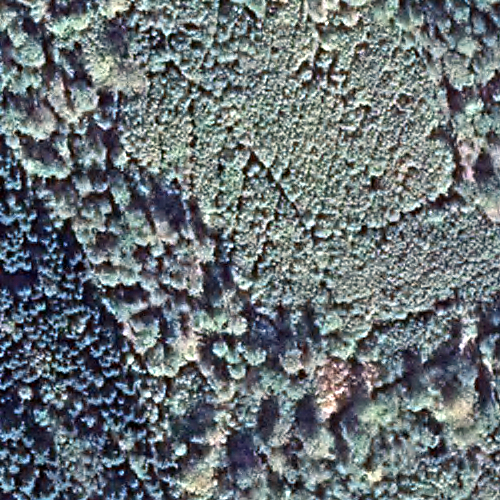
\includegraphics[width=0.465\textwidth]{Figures/C3/S3/ss1/RGB}
\label{subfig:C3_S3_ss1_sega}
}
\hspace*{0.025\textwidth}
\subfloat[nDSM.]{
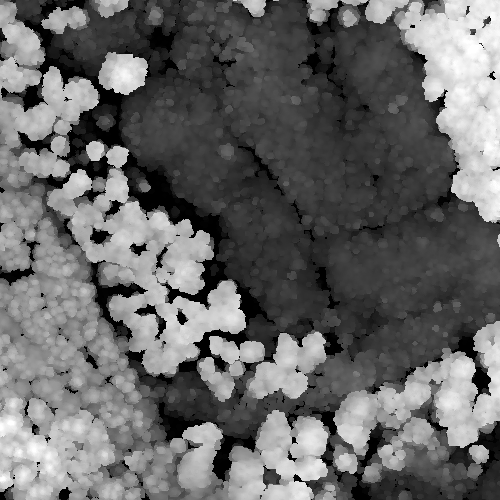
\includegraphics[width=0.465\textwidth]{Figures/C3/S3/ss1/nDSM}
\label{subfig:C3_S3_ss1_segb}
}
\endgroup
\\
\begingroup
\captionsetup[subfigure]{width=0.3\textwidth}
\subfloat[Tree extraction.]{
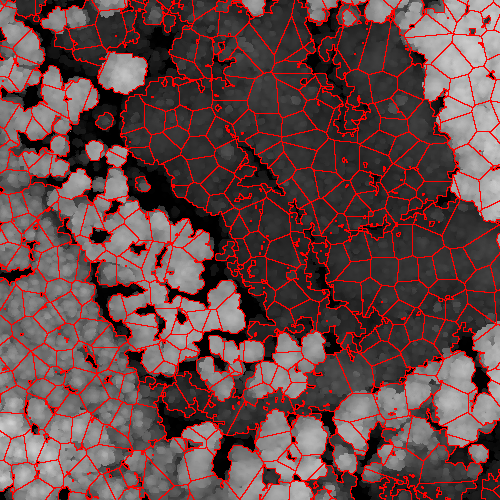
\includegraphics[width=0.3\textwidth]{Figures/C3/S3/ss1/nDSM_tree}
\label{subfig:C3_S3_ss1_segc}
}
\hspace*{0.025\textwidth}
\subfloat[Watershed.]{
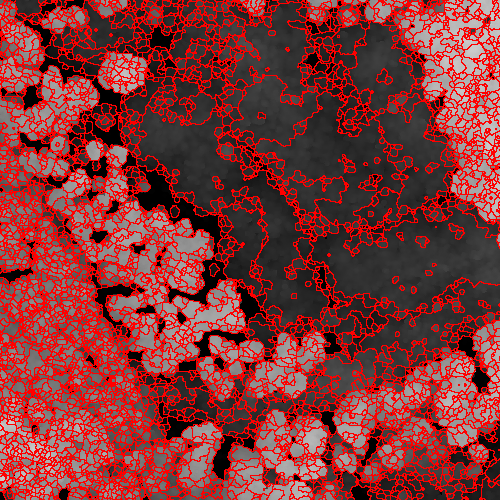
\includegraphics[width=0.3\textwidth]{Figures/C3/S3/ss1/nDSM_watershed}
\label{subfig:C3_S3_ss1_segd}
}
\hspace*{0.025\textwidth}
\subfloat[Hierarchical segmentation.]{
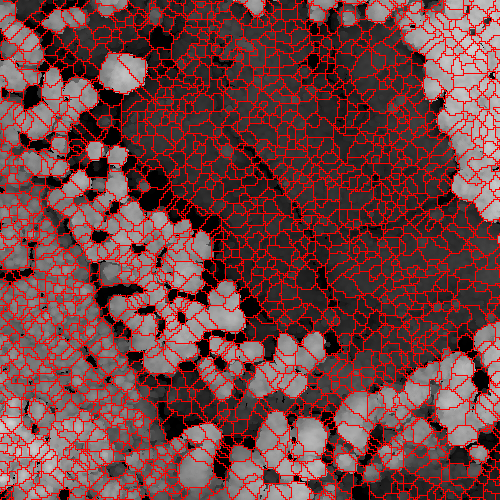
\includegraphics[width=0.3\textwidth]{Figures/C3/S3/ss1/nDSM_hierarchical}
\label{subfig:C3_S3_ss1_sege}
}
\\
\subfloat[PFF.]{
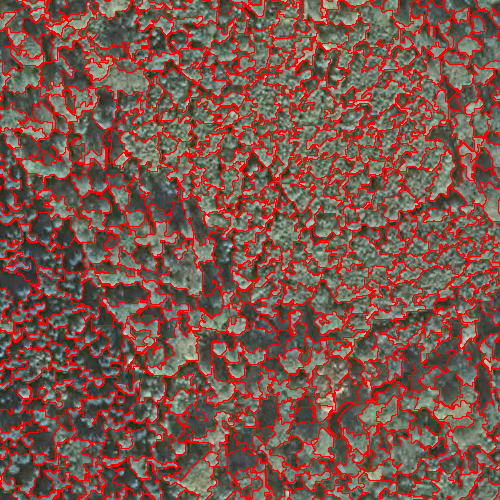
\includegraphics[width=0.3\textwidth]{Figures/C3/S3/ss1/PFF}
\label{subfig:C3_S3_ss1_segf}
}
\hspace*{0.025\textwidth}
\subfloat[Quickshift.]{
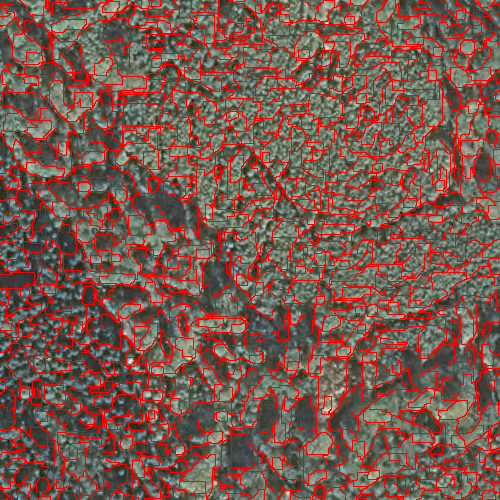
\includegraphics[width=0.3\textwidth]{Figures/C3/S3/ss1/quickshift}
\label{subfig:C3_S3_ss1_segg}
}
\hspace*{0.025\textwidth}
\subfloat[SLIC.]{
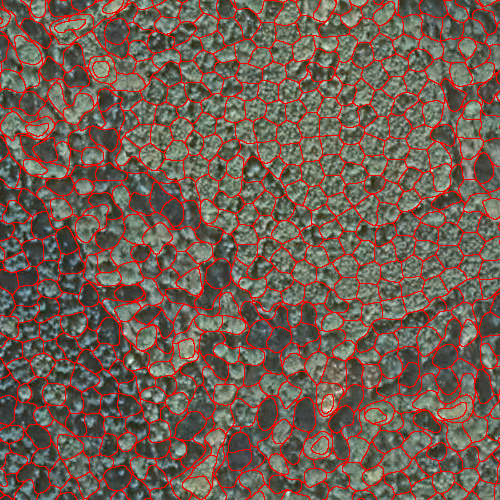
\includegraphics[width=0.3\textwidth]{Figures/C3/S3/ss1/SLIC}
\label{subfig:C3_S3_ss1_segh}
}

\endgroup
\caption{Over segmentation results, red corresponds to the borders found by the segmentation algorithm.}
\label{fig:C3_S3_ss1_seg}
\end{center}
\end{figure}

In all the proposed methods, the resulting segments are relevant since the all represent small homogeneous objects. The object are mostly not of the same size and shape, except for the SLIC superpixels (the aims of the methods is to obtain such uniform segments). The PFF algorithm produces objects with rough borders that are following precisely the borders observed on the images. From a visual point of view, it appears that there is no segmentation method that performs better than the others. Furthermore, it is impossible to evaluate the segmentation since no ground truth is available. Thus, the different segmentation methods are compared through the results they produce after the object-based classification (which indicates how the objects are relevant for classification) and after the regularization (how the objects impacts the final results). These results are presented in Figure~\ref{fig:C3_S3_ss1_results}\\

\begin{figure}[htbp]
\begin{center}
\begingroup
\captionsetup[subfigure]{width=0.21\textwidth}
\subfloat[IRC VHR \hbox{optical image}.]{
\includegraphics[width=0.3\textwidth]{Figures/C3/S3/ss1/classif_regul/IRC}
\label{subfig:C3_S3_ss1_resultsa}
}
\hspace*{0.025\textwidth}
\subfloat[nDSM.]{
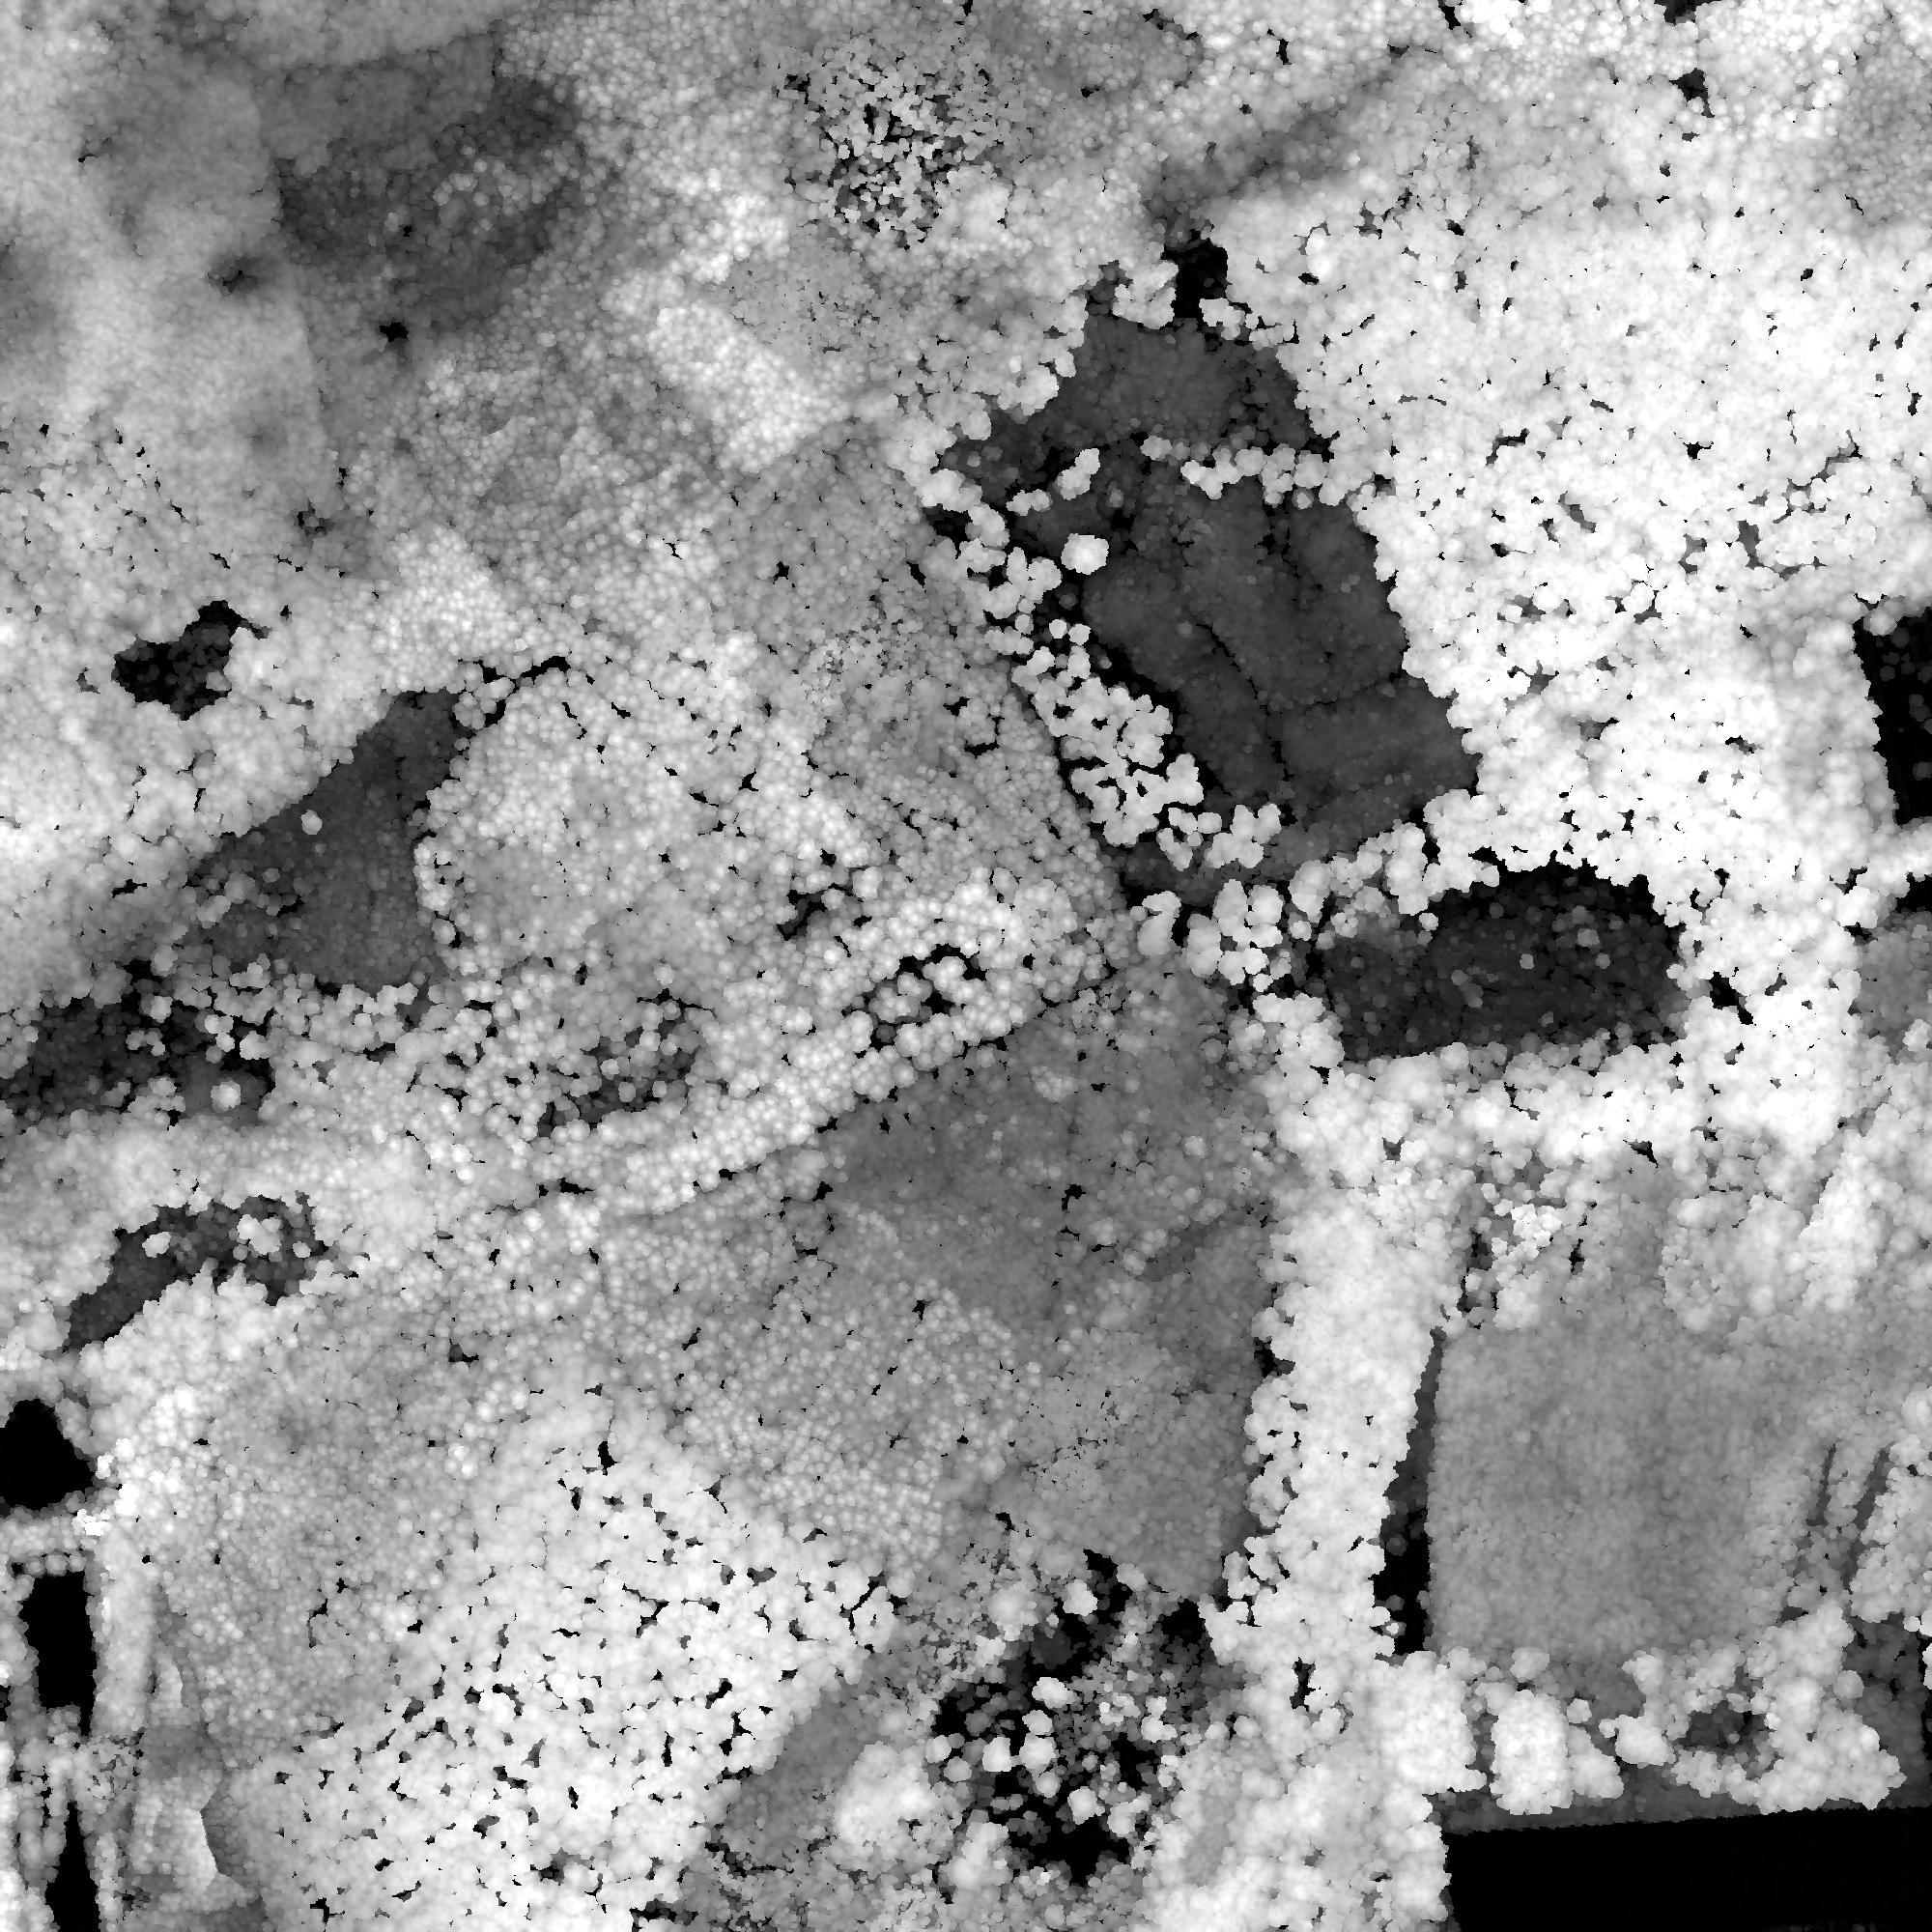
\includegraphics[width=0.3\textwidth]{Figures/C3/S3/ss1/classif_regul/nDSM}
\label{subfig:C3_S3_ss1_resultsb}
}
\hspace*{0.025\textwidth}
\subfloat[Forest LC.]{
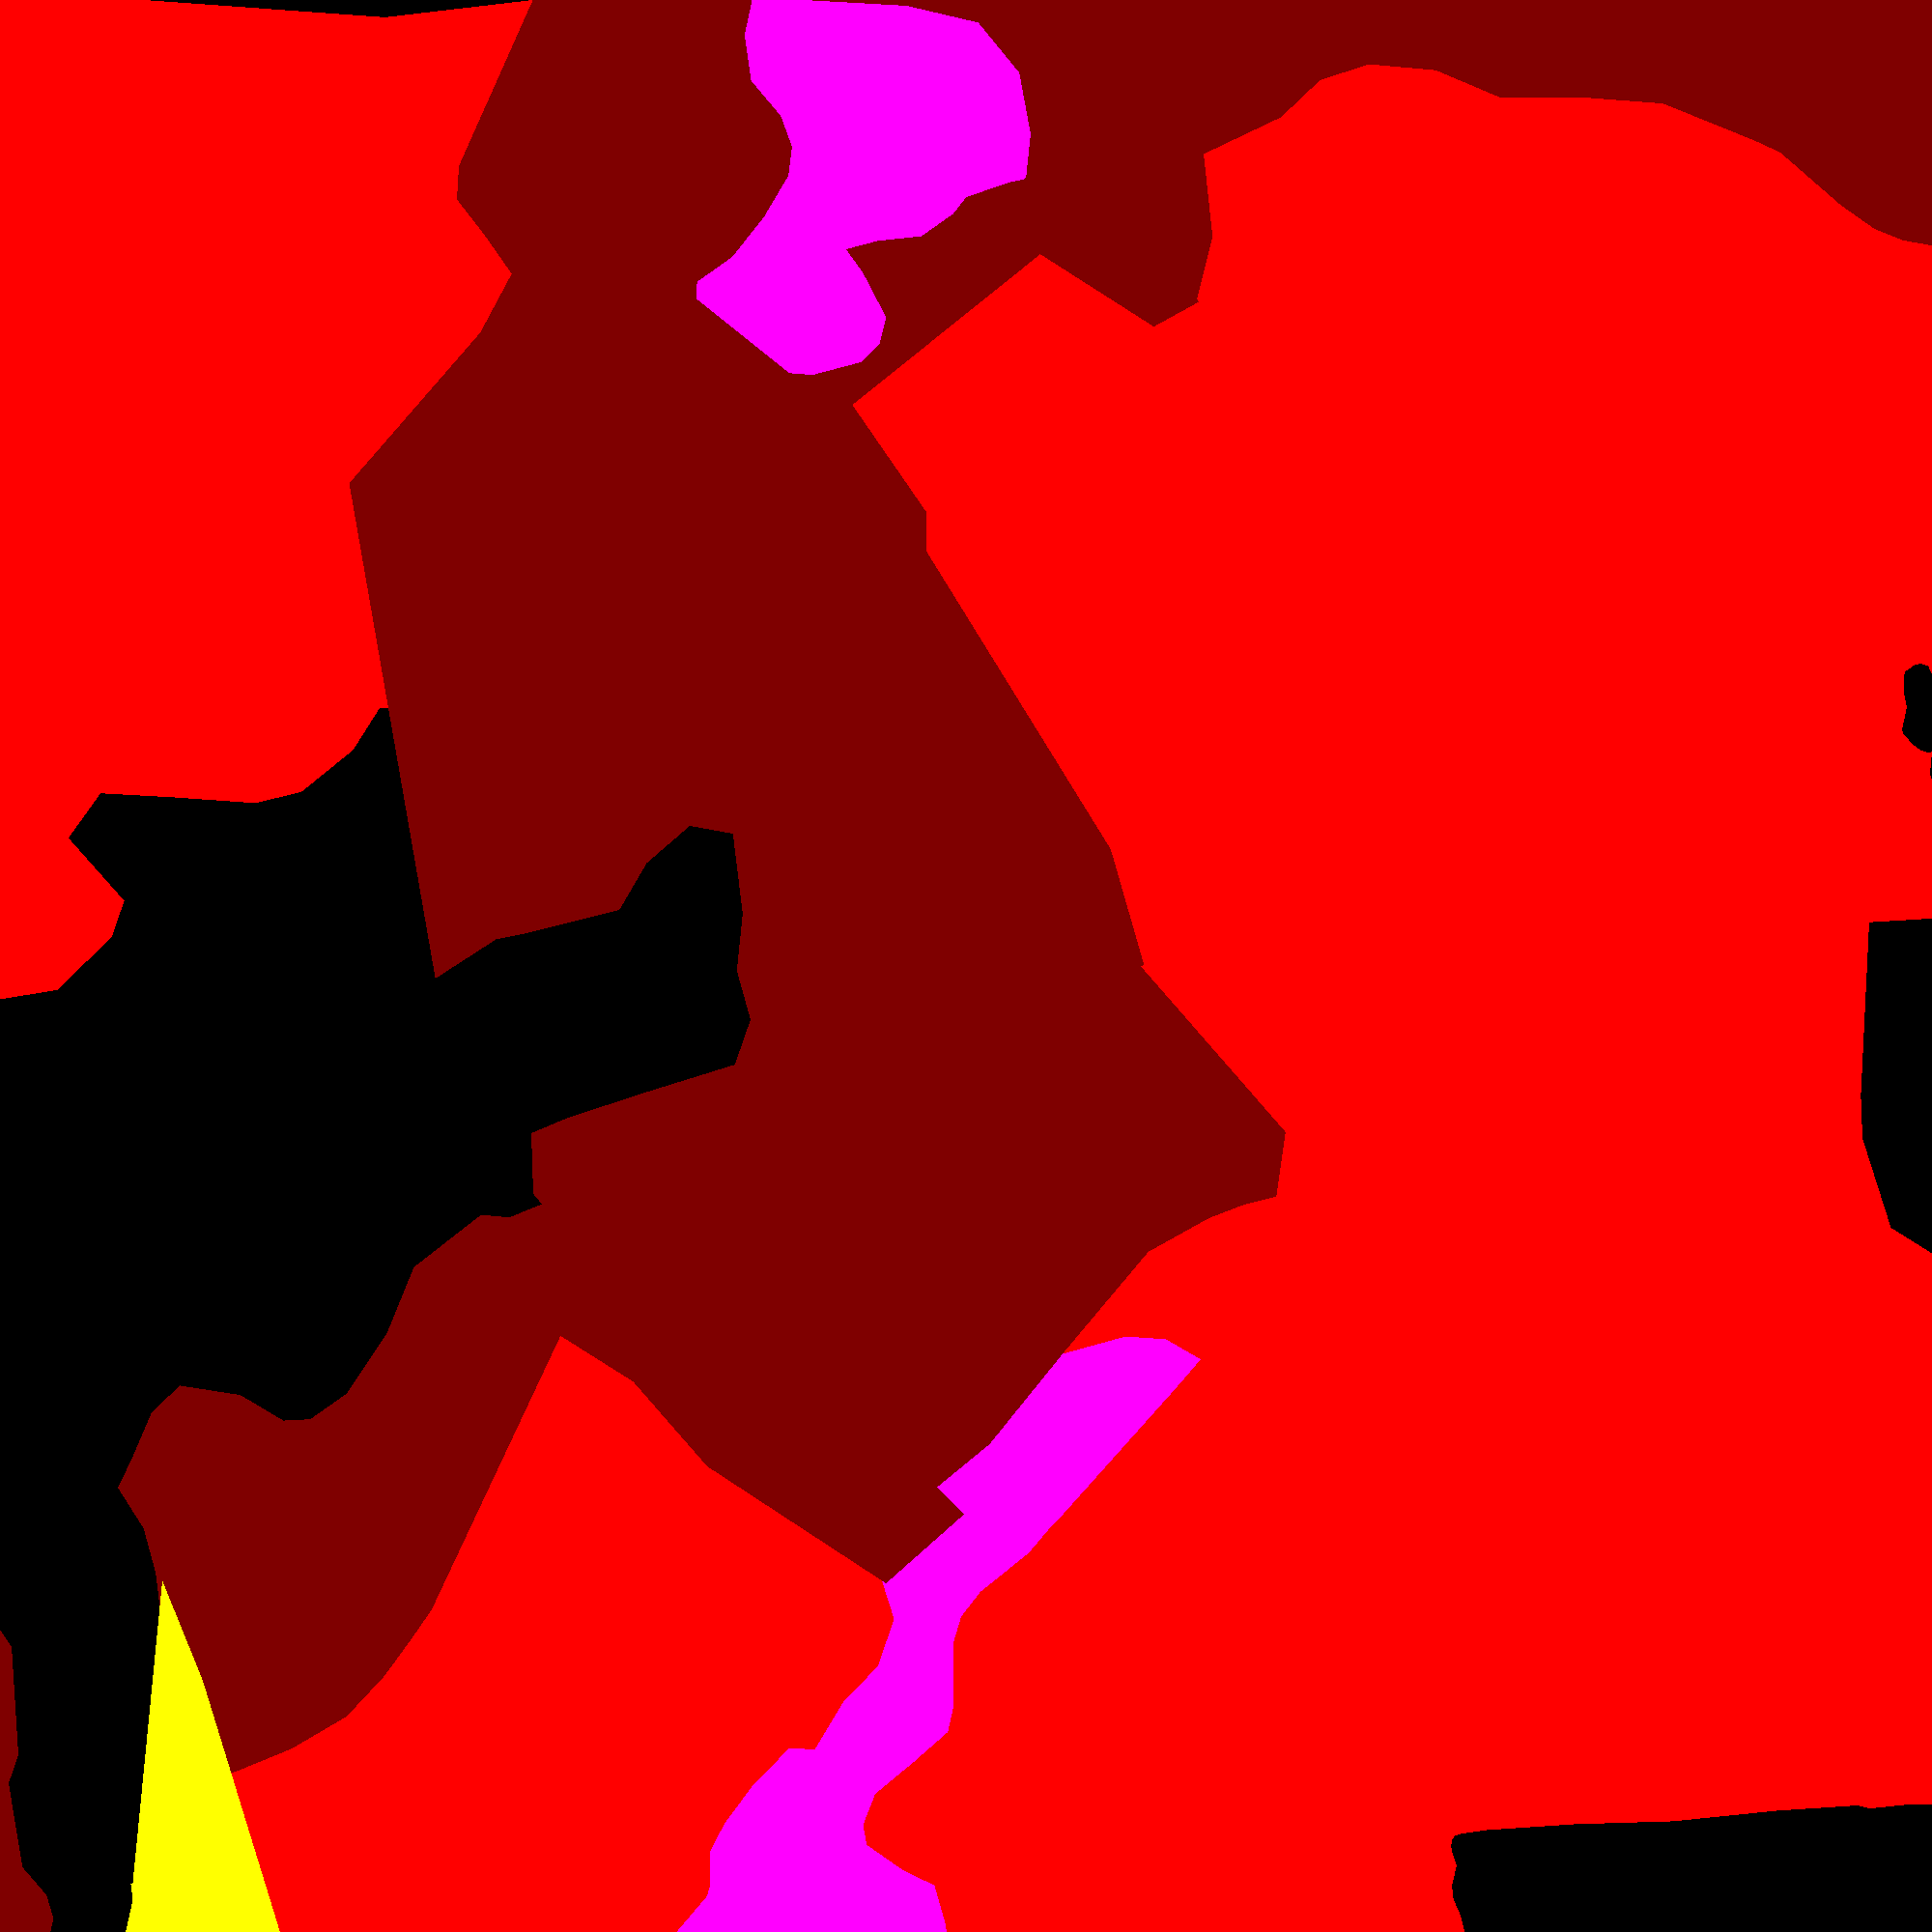
\includegraphics[width=0.3\textwidth]{Figures/C3/S3/ss1/classif_regul/BD}
\label{subfig:C3_S3_ss1_resultsc}
}
\\
\subfloat[Tree extraction.]{

\includegraphics[width=0.3\textwidth]{Figures/C3/S3/ss1/classif_regul/trees/regul}
\label{subfig:C3_S3_ss1_resultsd}
}
\hspace*{0.025\textwidth}
\subfloat[Watershed.]{

\includegraphics[width=0.3\textwidth]{Figures/C3/S3/ss1/classif_regul/watershed/regul}
\label{subfig:C3_S3_ss1_resultse}
}
\hspace*{0.025\textwidth}
\subfloat[Hierarchical \hbox{segmentation}.]{

\includegraphics[width=0.3\textwidth]{Figures/C3/S3/ss1/classif_regul/hierarchical/regul}
\label{subfig:C3_S3_ss1_resultsf}
}
\\
\subfloat[PFF.]{
\includegraphics[width=0.3\textwidth]{Figures/C3/S3/ss1/classif_regul/PFF/regul}
\label{subfig:C3_S3_ss1_resultsg}
}
\hspace*{0.025\textwidth}
\subfloat[Quickshift.]{
\includegraphics[width=0.3\textwidth]{Figures/C3/S3/ss1/classif_regul/quickshift/regul}
\label{subfig:C3_S3_ss1_resultsh}
}
\hspace*{0.025\textwidth}
\subfloat[SLIC.]{
\includegraphics[width=0.3\textwidth]{Figures/C3/S3/ss1/classif_regul/SLIC/regul}
\label{subfig:C3_S3_ss1_resultsi}
}

\endgroup
\caption{Over segmentation results.}
\label{fig:C3_S3_ss1_results}
\end{center}
\end{figure}


\subsection{Feature selection}

The feature selection have been carried out for 4 main reasons.
\begin{itemize}
\item It allows to determine how many feature are needed for an optimal classification.
\item It shows the complementarity of the data (optical images and lidar).
\item It permits to understand which feature are interesting for tree species classification.
\item It reduces the computational loads and times.
\end{itemize}

\paragraph{How many features for the classification? \\}
The idea here is to obtain the number feature for an optimal classification. The idea is to run the feature selection $N$ times using all the feature. Let $a_{n,k}$ be an accuracy metric for the classification of the $n^{\text{th}}$ iteration using the $k$ ($k \in [1,K]$) best features.
The optimal number of feature $k_{opt}$ is defined as follow:
\begin{equation}
\forall k \in [1,K], \quad \sum_{n=1}^{N}a_{n,k} \leq \sum_{n=1}^{N}a_{n,k_{opt}}
\end{equation}
Here, $K=95$ and $N=50$. This experiment have been carried out on different areas, and the optimal number of feature found is $k_{opt}=20$. Thus, in all the following experiments, the classification is performed using only 20 features.

\paragraph{Complementarity of the data. \\}
Once the optimal number of features was determined, the feature selection was performed 40 times over all the test areas in order to retrieve the most relevant features. The retained attributes are presented in Figures~\ref{fig:sel_lidar},\ref{fig:sel_spectral} and~\ref{fig:sel_indices}. On average, 61\% of the selected features are derived from the spectral information and 39\% from the lidar information for a single selection (i.e., in a random selection of 20 features, 12 are derived from VHR optical images and 8 from lidar). This shows the complementarity of both remote sensing data. 

\paragraph{Features for tree species classification. \\}
For the spectral information, the features derived from the original band set are more relevant than the vegetation indices: the near-infrared derived features represent 18\% of the spectral selected features, 16\% for the red and the green, 15\% for the blue and the DVI, only 11\% for the NDVI and 10\% for the RVI. 

The most relevant statistical feature for the spectral information is the minimum (17\% of the spectral selection). The maximum (12\%), the median (11\%), the mean (11\%) and the standard deviation (10\%) are also relevant. The other statistics are selected at less than 9\% each. For more details see Figure~\ref{fig:sel_spectral} and~\ref{fig:sel_indices}. \\

For the lidar information, the most relevant feature is surprisingly the intensity, selected in each of the 40 selections (12\% of the lidar selection, 5\% of the total selection). The standard deviation (8\% of the lidar selection), the maximum (7\%) and the densities (5\% and 6\%) are also relevant. The other lidar derived features count for less than 4\% each. For more details, see Figure~\ref{fig:sel_lidar}.

\paragraph{Reduce computational loads and times. \\}
It is obvious that processing a reduced number of features (20 instead of 95) reduces the computational loads and times. Furthermore, if an optimal subset of feature is found, only the concerned features need to be computed. Thus, the feature computation step would be reduced to a minimum step by computing only the relevant features.


\pgfplotstableread[col sep=comma,header=true]{
Sel, n
{z},11
{density1},16
{density2},20
{planarity},11
{scatter},6
{min},10
{max},23
{mean},7
{median},9
{standard deviation},24
{medADmed},14
{meanADmed},14
{skewness},4
{kurtosis},7
{10th percentile},8
{20th percentile},9
{30th percentile},10
{40th percentile},9
{50th percentile},7
{60th percentile},11
{70th percentile},12
{80th percentile},8
{90th percentile},11
{95th percentile},8
{intensity},40
}\datalidar

\begin{figure}[htbp]
\begin{center}
    \begin{tikzpicture}
    {
        \begin{axis}[    
            width=0.75\textwidth,
            xbar,                                 
            xtick={0,5,10,...,45},    
            xmin=0,
            xmax=45,       
            grid=major,
            nodes near coords, nodes near coords align={horizontal},
            symbolic y coords={intensity, 95th percentile, 90th percentile, 80th percentile, 70th percentile, 60th percentile, 50th percentile, 40th percentile, 30th percentile, 20th percentile, 10th percentile, kurtosis, skewness, meanADmed, medADmed, standard deviation, median, mean, max, min, scatter, planarity, density2, density1, z},
            ylabel={Features},
            ytick=data,
            xlabel={Number of selections},
            y label style={at={(-0.33,0.5)}},
            enlarge x limits={abs=0},
            y=0.025\textheight,
            reverse legend
        ]
        \addplot[color=black, fill=black!80!white] table [x=n, y=Sel] {\datalidar};
        \end{axis}
    }
    \end{tikzpicture}
\caption{Result of the feature selection for the lidar features over 40 trials of 20 optimal features.}
\label{fig:sel_lidar}
\end{center}
\end{figure}

%\pgfplotstableread[col sep=comma,header=true]{
%Sel, n
%{z},11
%{density1},16
%{density2},20
%{planarity},11
%{scatter},6
%{min},10
%{max},23
%{mean},7
%{median},9
%{standard deviation},24
%{medADmed},14
%{meanADmed},14
%{skewness},4
%{kurtosis},7
%{10$^{\text{th}}$percentile},8
%{20$^{\text{th}}$percentile},9
%{30$^{\text{th}}$percentile},10
%{40$^{\text{th}}$percentile},9
%{50$^{\text{th}}$percentile},7
%{60$^{\text{th}}$percentile},11
%{70$^{\text{th}}$percentile},12
%{80$^{\text{th}}$percentile},8
%{90$^{\text{th}}$percentile},11
%{95$^{\text{th}}$percentile},8
%{intensity},40
%}\datalidar
%
%\begin{figure}[htbp]
%\begin{center}
%    \begin{tikzpicture}
%    {
%        \begin{axis}[    
%            width=0.75\textwidth,
%            xbar,                                 
%            xtick={0,5,10,...,45},    
%            xmin=0,
%            xmax=45,       
%            grid=major,
%            nodes near coords, nodes near coords align={horizontal},
%            symbolic y coords={intensity, 95$^{\text{th}}$percentile, 90$^{\text{th}}$percentile, 80$^{\text{th}}$percentile, 70$^{\text{th}}$percentile, 60$^{\text{th}}$percentile, 50$^{\text{th}}$percentile, 40$^{\text{th}}$percentile, 30$^{\text{th}}$percentile, 20$^{\text{th}}$percentile, 10$^{\text{th}}$percentile, kurtosis, skewness, meanADmed, medADmed, standard deviation, median, mean, max, min, scatter, planarity, density2, density1, z},
%            ylabel={Features},
%            ytick=data,
%            xlabel={Number of selections},
%            y label style={at={(-0.33,0.5)}},
%            enlarge x limits={abs=0},
%            y=0.025\textheight,
%            reverse legend
%        ]
%        \addplot[color=black, fill=black!80!white] table [x=n, y=Sel] {\datalidar};
%        \end{axis}
%    }
%    \end{tikzpicture}
%\caption{Result of the feature selection for the lidar features over 40 trials of 20 optimal features.}
%\label{fig:sel_lidar}
%\end{center}
%\end{figure}
%
\pgfplotstableread[col sep=comma,header=true]{
Sel, R, G, B, NIR
Band,8,5,8,6
min,15,15,11,18
max,15,6,8,14
mean,8,11,13,13
median,7,9,7,9
standard deviation,5,6,9,6
meanADmed,6,7,7,3
meanADmean,4,3,5,9
medADmed,8,6,5,6
medADmean,4,6,4,4
}\dataspectral

\begin{figure} [htbp]%
\begin{center}
    \begin{tikzpicture}     
        \begin{axis}[    
            width=0.75\textwidth,
            xbar,                                 
            xtick={0,5,10,...,20},    
            xmin=0,
            xmax=20,       
            grid=major,
            nodes near coords, nodes near coords align={horizontal},
            symbolic y coords={medADmean,medADmed,meanADmean,meanADmed,standard deviation,median,mean,max,min,Band},
            ylabel={Features},
            ytick=data,
            xlabel={Number of selections},
            y label style={at={(-0.33,0.5)}},
            enlarge x limits={abs=0},
            y=0.09\textheight,
            reverse legend,
        ]
        \addplot[color=black, fill=gray!80!white] table [x=NIR, y=Sel] {\dataspectral};
        \addplot[color=black, fill=blue!80!white] table [x=B, y=Sel] {\dataspectral};  
        \addplot[color=black, fill=green!80!white] table [x=G, y=Sel] {\dataspectral};
        \addplot[color=black, fill=red!80!white] table [x=R, y=Sel] {\dataspectral};
        \legend{NIR band, Blue band, Green band, Red band}
        \end{axis}
    \end{tikzpicture}
\caption{Result of the feature selection for the spectral features over 40 trials of 20 optimal features.}
\label{fig:sel_spectral}
\end{center}
\end{figure}

\pgfplotstableread[col sep=comma,header=true]{
Sel, NDVI, DVI, RVI
Band,6,3,2
min,7,11,8
max,6,5,5
mean,2,3,3
median,6,11,6
standard deviation,8,11,5
meanADmed,9,4,6
meanADmean,5,3,4
medADmed,3,10,6
medADmean,3,7,5
}\dataindices

\begin{figure} [htbp]%
\begin{center}
    \begin{tikzpicture}     
        \begin{axis}[    
            width=0.75\textwidth,
            xbar,                                 
            xtick={0,5,10,...,15},    
            xmin=0,
            xmax=15,       
            grid=major,
            nodes near coords, nodes near coords align={horizontal},
            symbolic y coords={medADmean,medADmed,meanADmean,meanADmed,standard deviation,median,mean,max,min,Band},
            ylabel={Features},
            ytick=data,
            xlabel={Number of selections},
            y label style={at={(-0.33,0.5)}},
            enlarge x limits={abs=0},
            y=0.075\textheight,
            reverse legend,
        ]
        \addplot[color=black, fill=i2!80!white] table [x=RVI, y=Sel] {\dataindices};  
        \addplot[color=black, fill=i1!80!white] table [x=DVI, y=Sel] {\dataindices};
        \addplot[color=black, fill=i0!80!white] table [x=NDVI, y=Sel] {\dataindices};
        \legend{RVI, DVI, NDVI}
        \end{axis}
    \end{tikzpicture}
\end{center}
\caption{Result of the feature selection for the vegetation indices features over 40 trials of 20 optimal features.}
\label{fig:sel_indices}
\end{figure}


\subsection{Classification}
The classification is composed of two steps, the selection of training samples and the classification itself.
The classification is mainly performed using standard RF classifier \citep{opencv}. Tests have also been conducted using a SVM classifier with RBF kernel \citep{vapnik2013nature}. The classification can be impacted by two factors:
\begin{itemize}
\item The selection or non-selection of training pixels.
\item The object-based or pixel-based analysis.
\end{itemize}

\paragraph{Pixel-based classification versus object-based classification. \\}
The results of pixel-based and object-based classification is presented in Figure~\ref{fig:C3_S3_ss3_po}. The corresponding confusion matrices and accuracy metrics are presented in Tables~\ref{table:C3_S3_ss3_classif_pixel} and~\ref{table:C3_S3_ss3_classif_PFF}.

\begin{figure}[htbp]
\begin{center}
\begingroup
\captionsetup[subfigure]{width=0.425\textwidth}
\subfloat[IRC VHR optical image.]{
\includegraphics[width=0.45\textwidth]{Figures/C3/S3/ss3/IRC}
\label{subfig:C3_S3_ss3_poa}
}
\hspace*{0.025\textwidth}
\subfloat[Forest LC.]{
\includegraphics[width=0.45\textwidth]{Figures/C3/S3/ss3/BD}
\label{subfig:C3_S3_ss3_pob}
}
\\
\subfloat[Pixel-based classification (overall accuracy: 70.48\%, $\kappa$: 0.50).]{
\includegraphics[width=0.45\textwidth]{Figures/C3/S3/ss3/classif_pixel}
\label{subfig:C3_S3_ss3_poc}
}
\hspace*{0.025\textwidth}
\subfloat[Object-based classification (PFF) (overall accuracy: 93.14\%, $\kappa$: 0.86).]{
\includegraphics[width=0.45\textwidth]{Figures/C3/S3/ss3/classif_PFF}
\label{subfig:C3_S3_ss3_pod}
}
\endgroup
\caption{Classification results; pixel-based versus object-based.}
\label{fig:C3_S3_ss3_po}
\end{center}
\end{figure}

The pixel-based classification (Figure~\ref{subfig:C3_S3_ss3_poc}) appears more noisy than the object-based classification (Figure~\ref{subfig:C3_S3_ss3_pod}). However, the pixel-based classification already provide good discrimination results. Conversely, even if the object are roughly extracted (no specific attention is paid to the relevance of the extracted objects), the object-based classification produces more spatially consistent labels. Such results impacts the final output (see Figure~\ref{fig:C3_S3_ss3_rpo} and Tables~\ref{table:C3_S3_ss3_regul_pixel} and~\ref{table:C3_S3_ss3_regul_PFF}).

\begin{figure}[htbp]
\begin{center}
\begingroup
\captionsetup[subfigure]{width=0.425\textwidth}
\subfloat[Regularization using pixel-based classification (overall accuracy: 91.94\%, $\kappa$: 0.85).]{
\includegraphics[width=0.45\textwidth]{Figures/C3/S3/ss3/regul_pixel}
\label{subfig:C3_S3_ss3_rpoa}
}
\hspace*{0.025\textwidth}
\subfloat[Regularization using object-based classification (PFF) (overall accuracy: 97.44\%, $\kappa$: 0.95).]{
\includegraphics[width=0.45\textwidth]{Figures/C3/S3/ss3/regul_PFF}
\label{subfig:C3_S3_ss3_rpob}
}
\endgroup
\caption{Regularization results; pixel-based classification versus object-based classification.}
\label{fig:C3_S3_ss3_rpo}
\end{center}
\end{figure}

\paragraph{Training set design. \\}

The selection of the training pixels is an important step for the classification. It is a two sided problem:
\begin{itemize}
\item If the selected pixels are randomly taken from the polygons of the forest LC, some might not correspond to the target class, leading to confusion in the final classification.
\item If the pixels are selected using a too discriminative criteria, the variability of the target class will not be taken into account, also leading to confusion in the final classification.
\end{itemize}

The Figure~\ref{fig:C3_S3_ss3_sel} shows the pixels that have been selected by the k-mean algorithm for the training. Most of the pixel from the forest LC are retained. However, the pixels that are excluded from the training are visually relevant. Indeed, they mostly correspond to:
\begin{itemize}
\item Shadows from the optical images,
\item gaps in the canopy (retrieved from the lidar data),
\item pixels that are visually different from the other pixels of the considered class (i.e. other species).
\end{itemize}

The selection of training pixels is beneficial since it allows to remove the obviously irrelevant pixels from the training set while maintaining a certain variability within classes.

\begin{figure}[htbp]
\begin{center}
\begingroup
\captionsetup[subfigure]{width=0.45\textwidth}
\subfloat[RGB VHR optical image.]{
\includegraphics[width=0.45\textwidth]{Figures/C3/S3/ss3/RGB}
\label{subfig:C3_S3_ss_sela}
}
\hspace*{0.025\textwidth}
\subfloat[nDSM.]{
\includegraphics[width=0.45\textwidth]{Figures/C3/S3/ss3/nDSM}
\label{subfig:C3_S3_ss3_selb}
}
\\
\subfloat[Forest LC.]{
\includegraphics[width=0.45\textwidth]{Figures/C3/S3/ss3/BD}
\label{subfig:C3_S3_ss_selc}
}
\hspace*{0.025\textwidth}
\subfloat[Retained pixels for training.]{
\includegraphics[width=0.45\textwidth]{Figures/C3/S3/ss3/training_set}
\label{subfig:C3_S3_ss3_seld}
}
\endgroup
\caption{Selection of the training pixels.}
\label{fig:C3_S3_ss3_sel}
\end{center}
\end{figure}

The results of the classification and regularization using different training set is presented in Figure~\ref{fig:C3_S3_ss3_sel_results}. The confusion matrices and accuracy metrics when the training pixels are not selected are presented in Tables~\ref{table:C3_S3_ss3_classif_without_training} and~\ref{table:C3_S3_ss3_regul_without_training}.

\begin{figure}[htbp]
\begin{center}
\begingroup
\captionsetup[subfigure]{width=0.45\textwidth}
\subfloat[Classification with selection of training pixels  (overall accuracy: 93.14\%, $\kappa$: 0.86).]{
\includegraphics[width=0.45\textwidth]{Figures/C3/S3/ss3/classif_PFF}
\label{subfig:C3_S3_ss3_sel_resultsa}
}
\hspace*{0.025\textwidth}
\subfloat[Regularization  with selection of training pixels (overall accuracy: 97.44\%, $\kappa$: 0.95).]{
\includegraphics[width=0.45\textwidth]{Figures/C3/S3/ss3/regul_PFF}
\label{subfig:C3_S3_ss3_sel_resultsb}
}
\\
\subfloat[Classification without selection of training pixels (overall accuracy: 78.98\%, $\kappa$: 0.62).]{
\includegraphics[width=0.45\textwidth]{Figures/C3/S3/ss3/classif_without_training}
\label{subfig:C3_S3_ss3_sel_resultsc}
}
\hspace*{0.025\textwidth}
\subfloat[Regularization without selection of training pixels (overall accuracy: 94.67\%, $\kappa$: 0.89).]{
\includegraphics[width=0.45\textwidth]{Figures/C3/S3/ss3/regul_without_training}
\label{subfig:C3_S3_ss3_sel_resultsd}
}
\endgroup
\caption{Selection of the training pixels.}
\label{fig:C3_S3_ss3_sel_results}
\end{center}
\end{figure}

The selection of training pixels greatly increases the classification results. Indeed, without any selection, the classification is very noisy (even when working at the object level) and many confusion are reported. The regularization attenuates the errors, but the result remains worse than the one obtained with the selection of training pixels.

\subsection{Regularization}
The smoothing of the classification can be performed using local or global methods.

\subsubsection{Local methods}
Two methods have been investigated for the local smoothing of the classification. They are very easy to implement and have low computation times.
Firstly, the use of a majority filter have been employed. Since it does not take into account the probabilities, a probabilistic relaxation have then also been tested. For both method, the main problem is to defined a relevant neighborhood size. If if is too small, the results will remain noisy, and if it is too important, the results will be over generalized and the computational times will explode.

\paragraph{Majority filter. \\}
The results for the majority filter is presented in Figure~\ref{fig:C3_S3_ss4_maj}.  The filtering method performs the worse with a gain of less than 1\% compared to the classification, even with large filters. Furthermore,the larger the filter is,the longer are the computation times. 

\begin{figure}[htbp]
\begin{center}
\begingroup
\captionsetup[subfigure]{width=0.3\textwidth}
\subfloat[Forest LC database.]{
\includegraphics[width=0.3\textwidth]{Figures/C3/S3/ss4/BD}
\label{subfig:C3_S3_ss4_maja}
}
\hspace*{0.025\textwidth}
\subfloat[Majority filter ($r=5$).]{
\includegraphics[width=0.3\textwidth]{Figures/C3/S3/ss4/local/filter/5/filter}
\label{subfig:C3_S3_ss4_majb}
}
\hspace*{0.025\textwidth}
\subfloat[Majority filter ($r=25$).]{
\includegraphics[width=0.3\textwidth]{Figures/C3/S3/ss4/local/filter/25/filter}
\label{subfig:C3_S3_ss4_majc}
}
\endgroup
\caption{Results of the majority filters.}
\label{fig:C3_S3_ss4_maj}
\end{center}
\end{figure}

\paragraph{Probabilistic relaxation. \\}
The results for the probabilistic relaxation is presented in Figure~\ref{fig:C3_S3_ss4_prob}. The probabilistic relaxation has also poor results (+5\% than the classification) and has also important computation times, since the iterative process runs until the convergence has been reached.

\begin{figure}[htbp]
\begin{center}
\begingroup
\captionsetup[subfigure]{width=0.425\textwidth}
\subfloat[Forest LC database.]{
\includegraphics[width=0.45\textwidth]{Figures/C3/S3/ss4/BD}
\label{subfig:C3_S3_ss4_proba}
}
\hspace*{0.025\textwidth}
\subfloat[Probabilistic relaxation ($r=5$).]{
\includegraphics[width=0.45\textwidth]{Figures/C3/S3/ss4/local/relax/relax}
\label{subfig:C3_S3_ss4_probb}
}
\endgroup
\caption{Results of the probabilistic relaxation.}
\label{fig:C3_S3_ss4_prob}
\end{center}
\end{figure}

\subsubsection{Global methods}
The regularization is the final step that smooth the former classification. In the formulation of the energy, 3 aspect are taken into account. The two most important are the integration of the information from the classification (unary term) and how the feature are integrated into the smoothing process (prior). The last aspect is the integration of other constraints, allowed by the use of the QPBO algorithm.

The global methods produce significantly better results than the local methods.

The effect of the parameter $\gamma$ is presented in Figure~\ref{fig:C3_S3_ss4_gamma}. When $\gamma$ is low, the borders are rough and small regions might appear (Figure~\ref{subfig:C3_S3_ss4_gammac}). Increasing $\gamma$ smooth the borders, however, a too high value have a negative impact on the results, reducing the size of meaningful segments (Figure~\ref{subfig:C3_S3_ss4_gammae}) or even removing them (Figure~\ref{subfig:C3_S3_ss4_gammaf}). The tuning of the parameter $\gamma$ is an important issue, since different values of $\gamma$ might be acceptable depending on the level of detail expected for the segmentation. In forest inventory, having small regions of pure species is interesting for the understanding of the behavior of the forest. For generalization purposes (such as forest LC), the segments must have a decent size and may exhibit variability.

\begin{figure}[htbp]
\begin{center}
\begingroup
\captionsetup[subfigure]{width=0.45\textwidth}
\subfloat[IRC VHR optical image.]{
\includegraphics[width=0.45\textwidth]{Figures/C3/S3/ss4/IRC}
\label{subfig:C3_S3_ss4_gammaa}
}
\hspace*{0.025\textwidth}
\subfloat[Forest LC.]{
\includegraphics[width=0.45\textwidth]{Figures/C3/S3/ss4/BD}
\label{subfig:C3_S3_ss4_gammab}
}
\\
\subfloat[Regularization ($\gamma=5$).]{
\includegraphics[width=0.45\textwidth]{Figures/C3/S3/ss4/gamma/5/regul}
\label{subfig:C3_S3_ss4_gammac}
}
\hspace*{0.025\textwidth}
\subfloat[Regularization ($\gamma=10$).]{
\includegraphics[width=0.45\textwidth]{Figures/C3/S3/ss4/gamma/10/regul}
\label{subfig:C3_S3_ss4_gammad}
}
\\
\subfloat[Regularization ($\gamma=15$).]{
\includegraphics[width=0.45\textwidth]{Figures/C3/S3/ss4/gamma/15/regul}
\label{subfig:C3_S3_ss4_gammae}
}
\hspace*{0.025\textwidth}
\subfloat[Regularization ($\gamma=20$).]{
\includegraphics[width=0.45\textwidth]{Figures/C3/S3/ss4/gamma/20/regul}
\label{subfig:C3_S3_ss4_gammaf}
}
\endgroup
\caption{Regularization results, effect of the parameter $\gamma$.}
\label{fig:C3_S3_ss4_gamma}
\end{center}
\end{figure}

\paragraph{Unary term. \\}

The unary term have the major impact on the regularization results (see Figure~\ref{fig:C3_S3_ss4_unary}). Indeed, the log-inverse formulation highly penalize pixels with low probability, thus, small areas with high probabilities will be kept, even with an important $\gamma$. Contrarily, the linear formulation have a stronger smoothing effect.

\begin{figure}[htbp]
\begin{center}
\begingroup
\captionsetup[subfigure]{width=0.3\textwidth}
\subfloat[Forest LC database.]{
\includegraphics[width=0.3\textwidth]{Figures/C3/S3/ss4/BD}
\label{subfig:C3_S3_ss4_unarya}
}
\hspace*{0.025\textwidth}
\subfloat[Regularization results using the log-inverse data formulation.]{
\includegraphics[width=0.3\textwidth]{Figures/C3/S3/ss4/data/log/regul}
\label{subfig:C3_S3_ss4_unaryb}
}
\hspace*{0.025\textwidth}
\subfloat[Regularization results using the linear data formulation.]{
\includegraphics[width=0.3\textwidth]{Figures/C3/S3/ss4/data/linear/regul}
\label{subfig:C3_S3_ss4_unaryc}
}
\endgroup
\caption{Impact of the formulation of the unary term.}
\label{fig:C3_S3_ss4_unary}
\end{center}
\end{figure}

Both are interesting for the analysis of forest. The log-inverse allows to obtain small areas that keep an important class confidence. Such areas are useful for forest inventory since they give information about large forested areas with small islets of pure species. Conversely, the linear formulation produces smooth segments that are more relevant for a national mapping.

\paragraph{Prior. \\}

The prior have a weak impact on the regularization results (see Figure~\ref{fig:C3_S3_ss4_prior}).

\begin{figure}[htbp]
\begin{center}
\begingroup
\captionsetup[subfigure]{width=0.3\textwidth}
\subfloat[Forest LC database.]{
\includegraphics[width=0.3\textwidth]{Figures/C3/S3/ss4/BD}
\label{subfig:C3_S3_ss4_priora}
}
\hspace*{0.025\textwidth}
\subfloat[Regularization results using the \textit{Potts model}.]{
\includegraphics[width=0.3\textwidth]{Figures/C3/S3/ss4/binary/potts/regul}
\label{subfig:C3_S3_ss4_priorb}
}
\hspace*{0.025\textwidth}
\subfloat[Regularization results using the \textit{z-Potts model}.]{
\includegraphics[width=0.3\textwidth]{Figures/C3/S3/ss4/binary/cs/regul}
\label{subfig:C3_S3_ss4_priorc}
}
\\
\subfloat[Regularization results using the \textit{Exponential-features model}.]{
\includegraphics[width=0.3\textwidth]{Figures/C3/S3/ss4/binary/ef/regul}
\label{subfig:C3_S3_ss4_priord}
}
\hspace*{0.025\textwidth}
\subfloat[Regularization results using the \textit{Distance-features model}.]{
\includegraphics[width=0.3\textwidth]{Figures/C3/S3/ss4/binary/df/regul}
\label{subfig:C3_S3_ss4_priore}
}
\endgroup
\caption{Impact of the formulation of the data term.}
\label{fig:C3_S3_ss4_prior}
\end{center}
\end{figure}

The \textit{z-Potts model} tends to have slightly worse results than the other methods. The \textit{Potts model} and the \textit{Distance-features model} have very close results regardless of the unary term. The \textit{Exponential-features model} have the greatest results with the linear unary, but have poor results with the log-inverse unary.

\paragraph{Adding constraints. \\}
The addition of constraints could be easily carried out with the QPBO algorithm. We can add strong borders that we want to retrieve in the final segmentation. Unfortunately, such borders can not be easily extracted (see Section~\ref{sec:C3_S2_ss1}). It is then not relevant to add such constraints since they will not lead to accurate results. 

A second constraint can be employed in order to ensure a minimal size of the final segments. However, it leads to three issues
\begin{enumerate}
\item The minimal size of a segment should be defined. Even if such minimal size is defined by the definition of forest stands (0.5$\:$ha), a segment with a size of 0.5$\:$ha$+$1 pixels will not be considered as a small segment.
\item If such constraint wants to be employed, the QPBO algorithm have to run until all the segments have reached the minimum size. Such iteration might be long
\item The final result will be similar to a majority vote. For a small segment, selecting the label of the neighbor segment that have the most neighbor pixels with the small segment will nearly lead to the same results of the regularization using minimal size constraint.
\end{enumerate}

\subsection{Importance of fusion}
In this framework, the fusion is performed at multiple levels;
\begin{itemize}
\item Choice of data for the over-segmentation,
\item Features employed for the classification,
\item Features employed for the regularization.
\end{itemize}

The impact of the choice of the data for the over-segmentation have already been investigated in Section~\ref{sec:C3_S3_ss1}. When employing an over-segmentation from VHR optical images (e.g. PFF, Quickshift or SLIC) or from a lidar data (e.g. hierarchical segmentation on nDSM or tree extraction) produces similar results. 

Experiments have been conducted in order to determine how the choice of the data impact both the classification and regularization step. In order to evaluate the impact of the data choice on the classification and regularization, 5 scenarii have been investigated:
\begin{itemize}
\item A full lidar scenario:
\begin{itemize}
\item Hierarchical segmentation on the nDSm,
\item Object-based classification (with selection of training samples) using the 25 lidar features,
\item Regularization using the 25 lidar features.
\end{itemize}
\item A full spectral scenario:
\begin{itemize}
\item PFF segmentation of the VHR optical image,
\item Object-based classification (with selection of training samples) using a selection of 20 spectral features,
\item Regularization using a selection of 20 spectral features.
\end{itemize}
\item 3 scenarii:
\begin{itemize}
\item PFF segmentation of the VHR optical image,
\item Object-based classification (with selection of training samples) using a selection of 20 features (lidar and spectral),
\end{itemize}
\begin{enumerate}
\item Regularization using the 25 lidar features,
\item Regularization using a selection of 20 spectral features,
\item Regularization using a selection of 20 features (lidar and spectral).
\end{enumerate}
\end{itemize}

The overall accuracies for these 5 scenarii are presented in Table~\ref{table:fusion_results}.

\begin{table}[htbp]
\begin{center}
\begin{footnotesize}
\begin{tabular}{|l|c|c|c|}
\hline
\multirow{2}{*}{Scenario} & \multicolumn{3}{c|}{\textbf{Overall accuracy (\%)}} \\
\cline{2-4}
& Classification & Regularization & Gain \\
\hline
Full lidar & 74.8 & 92.2 & 17.4 \\
\hline
Full spectral & 79.1 & 95.2 & 16.1 \\
\hline
Regularization lidar & \multirow{3}{*}{87.6} & 96.0 & 8.4 \\
\cline{1-1} \cline{3-4}
Regularization spectral &  & 96.1 & 8.5 \\
\cline{1-1} \cline{3-4}
Regularization lidar + spectral &  & 96.2 & 8.6 \\
\hline
\end{tabular} \\
\end{footnotesize}
\end{center}
\vspace*{-5mm}
\caption{Classification and stand segmentation accuracies for the 5 scenarii investigated.}
\label{table:fusion_results}
\end{table}

The impact of the choice of the data on the classification is obvious; the classification using a single data source performs worse than when using both. Furthermore, the spectral information tends to be more relevant that the spectral information. Such results are coherent with the results of the feature selection since the spectral feature are selected for 61\% and for 39\% for the lidar.

The impact of the choice of the data on the regularization is less significant. We can first note that the use of a single modality can greatly improve the results from a poor classification (+17.4\% for lidar and +16.1\% for spectral). However, when the classification is already significant, the improvement is more or less the same. The spectral information is a bit more beneficial than the lidar information for the regularization step. Fusing the two data sources or using only the spectral information in the regularization step does not significantly change the final results.

\section{Co-products of the method}
The outputs of the method can be employed for further investigation in order to extract relevant information about forest. Firstly, the forest stands obtained can be employed for the semi-automatic update of the forest LC. Secondly, the information extracted from the original data can be employed for forest inventory.
\subsection{Semi-automatic update}
The semi-automatic update of the forest LC can be performed by the joint analysis of the final stand segmentation and the forest LC employed.

A change map can be derived and changes can be prioritized according to their size and shape.
Here 3 criteria are employed for an area of change :
\begin{itemize}
\item The number of pixels,
\item The size of the rectangular bounding box (see Figure~\ref{subfig:changesb}),
\item The size of the circular bounding box (see Figure~\ref{subfig:changesc}).
\end{itemize}

\begin{figure}[htbp]
\begin{center}
\begingroup
\captionsetup[subfigure]{width=0.3\textwidth}
\subfloat[Detected change]{
\includegraphics[width=0.3\textwidth]{Figures/C3/S4/ss1/area}
\label{subfig:changes}
}
\hfill
\subfloat[Rectangular bounding box of the change.]{
\includegraphics[width=0.3\textwidth]{Figures/C3/S4/ss1/area_rectangular}
\label{subfig:changesb}
}
\hfill
\subfloat[Circular bounding box of the change.]{
\includegraphics[width=0.3\textwidth]{Figures/C3/S4/ss1/area_circular}
\label{subfig:changesc}
}
\endgroup
\caption{Bounding boxes of the change detection.}
\label{fig:changes}
\end{center}
\end{figure}

The changes are classified using thresholds based on the size (in pixels) of the change $s$, the ratio between the size of the change and the size of the rectangular bounding box $r_{1}$ and  the ratio between the size of the change and the size of the circular bounding box $r_{2}$. An change is defined as major when the condition~(\ref{eq:c1}) or~(\ref{eq:c2}) is verified. 
\begin{eqnarray}
s \geq 100 \text{ and } r_{1} \geq 0.3, \label{eq:c1}\\
s \geq 100 \text{ and } r_{2} \geq 0.2. \label{eq:c2}
\end{eqnarray}

An "updated" forest LC can be then created, the area of major change are labeled as \textit{no data} (see Figure~\ref{fig:new_BD}). A difference map is also produced with two kinds of differences:
\begin{itemize}
\item The minor differences; they correspond to areas where the borders of the Forest LC does not exactly fit with the borders obtained in the method. This type of error is common since the border from the Forest LC are mostly strait lines while the methods tends to follow the natural borders of the forest because of the regularization.
\item The major differences; they correspond to large patches that differ from the Forest LC. Two cases can be differentiated:
\begin{itemize}
\item The method can have produced wrong results,
\item The forest has changed or has been exploited (cut or plantation).
\end{itemize}
\end{itemize}

\begin{figure}[htbp]
\begin{center}
\begingroup
\captionsetup[subfigure]{width=0.5\textwidth}
\subfloat[Forest LC.]{
\includegraphics[width=0.45\textwidth]{Figures/C3/S4/ss1/results/BD}
\label{subfig:new_BDa}
}
\hfill
\subfloat["Updated" Forest LC.]{
\includegraphics[width=0.45\textwidth]{Figures/C3/S4/ss1/results/BD_new}
\label{subfig:new_BDb}
}
\endgroup
\caption{Automatic update of the Forest LC.}
\label{fig:new_BD}
\end{center}
\end{figure}

In case of major change, the decision can be taken to keep the original forest LC or to employ the result of the method. An operator can also focus of the change and correct it manually (see Figure~\ref{fig:IRC_change})

\begin{figure}[htbp]
\begin{center}
\includegraphics[width=1.0\textwidth]{Figures/C3/S4/ss1/results/IRC_dif}
\caption{Detected changes of the Forest LC, green corresponds to major changes, blue corresponds to minor changes.}
\label{fig:IRC_change}
\end{center}
\end{figure}

\subsection{Inventory}
The features derived from lidar and the final stand segmentation

%----------------------------------------------------------------------------------------

% Define some commands to keep the formatting separated from the content 
%\newcommand{\keyword}[1]{\textbf{#1}}
%\newcommand{\tabhead}[1]{\textbf{#1}}
%\newcommand{\code}[1]{\texttt{#1}}
%\newcommand{\file}[1]{\texttt{\bfseries#1}}
%\newcommand{\option}[1]{\texttt{\itshape#1}}

%----------------------------------------------------------------------------------------


\stopcontents[chapters]
\openchapter
% Chapter 4

\chapter{Conclusion and perspectives} % Main chapter title
\label{Conclusion} % For referencing the chapter elsewhere, use \ref{Chapter1} 

\startcontents[chapters]
\Mprintcontents


%----------------------------------------------------------------------------------------

% Define some commands to keep the formatting separated from the content 
%\newcommand{\keyword}[1]{\textbf{#1}}
%\newcommand{\tabhead}[1]{\textbf{#1}}
%\newcommand{\code}[1]{\texttt{#1}}
%\newcommand{\file}[1]{\texttt{\bfseries#1}}
%\newcommand{\option}[1]{\texttt{\itshape#1}}

%----------------------------------------------------------------------------------------


\stopcontents[chapters]

%\includetex{Chapters/Chapter1}
%\includetex{Chapters/Chapter2} 
%\includetex{Chapters/Chapter3} 
%\includetex{Chapters/Conclusion}

%----------------------------------------------------------------------------------------
%	THESIS CONTENT - APPENDICES
%----------------------------------------------------------------------------------------

\appendix % Cue to tell LaTeX that the following "chapters" are Appendices

% Include the appendices of the thesis as separate files from the Appendices folder
% Uncomment the lines as you write the Appendices

\openchapter
% Appendix A

\chapter{Color code} % Main appendix title

\label{AppendixA} % For referencing this appendix elsewhere, use \ref{AppendixA}

\begin{table}
\begin{center}
\begin{tabular}{l l}
\p[l1] & {\textit{Chênes décidus}} \\
\p[l2] & {\textit{Chênes sempervirents}} \\
\p[l3] & {\textit{Hêtre}} \\
\p[l4] & {\textit{Châtaignier}} \\
\p[l5] & {\textit{Robinier}} \\
\p[l6] & {\textit{Autre feuillu pur}} \\
\p[l7] & {\textit{Pin maritime}} \\
\p[l8] & {\textit{Pin sylvestre}} \\
\p[l9] & {\textit{Pin laricio ou pin noir}} \\
\p[l10] & {\textit{Pin d'Alep}} \\
\p[l11] & {\textit{Pin à crochet ou pin cembro}} \\
\p[l12] & {\textit{Autre pin pur}} \\
\p[l13] & {\textit{Sapin ou épicéa}} \\
\p[l14] & {\textit{Mélèze}} \\
\p[l15] & {\textit{Douglas}} \\
\p[l16] & {\textit{Autre conifère pur autre que pin}} \\
\p[l17] & {\textit{Lande ligneuse}} \\
\p[l18] & {\textit{Formation herbacée}} \\
\p[l19] & {\textit{Peupleraie}} \\
\end{tabular}
\end{center}
\caption{Vegetation type color code}
\end{table}
\openchapter
% Appendix Template

\chapter{Publication} % Main appendix title

\label{Publication} % Change X to a consecutive letter; for referencing this appendix elsewhere, use \ref{AppendixX}

\startcontents[chapters]
\Mprintcontents


\section{Journal articles}

C. Dechesne, C. Mallet, A. Le Bris, V. Gouet-Brunet. \textit{Semantic segmentation of forest stands of pure species combining airborne lidar data and very high resolution multispectral imagery}. ISPRS Journal of Photogrammetry and Remote Sensing, 126 (2017), pp.129–145, 2017. \href{http://recherche.ign.fr/labos/matis/pdf/articles_revues/2017/semantic_segmentation.pdf}{\includegraphics[height=10pt]{Appendices/ic_pdf.jpg}} \\

M. Fauvel, C. Dechesne, A. Zullo, F. Ferraty. \textit{Fast forward feature selection of hyperspectral images for classification with gaussian mixture models}. IEEE Journal of Selected Topics in Applied Earth Observations and Remote Sensing, vol. 8(6), pp. 2824-2831, 2015. \href{https://arxiv.org/pdf/1501.00857v1.pdf}{\includegraphics[height=10pt]{Appendices/ic_pdf.jpg}} \\

\section{Peer-reviewed conference paper}

C. Dechesne, C. Mallet, A. Le Bris, V. Gouet-Brunet. \textit{How to combine LIDAR and very high resolution multispectral images for forest stand segmentation?} Proc. of the IEEE International Geoscience and Remote Sensing Symposium (IGARSS), Fort Worth, USA, July 2017. \href{http://recherche.ign.fr/labos/matis/pdf/articles_conf/2017/IGARSS_2017_Dechesne_Clement_final.pdf}{\includegraphics[height=10pt]{Appendices/ic_pdf.jpg}} \\

C. Dechesne, C. Mallet, A. Le Bris, V. Gouet-Brunet. \textit{Semantic segmentation of forest stands of pure specie as a global optimisation problem}. ISPRS Annals of the Photogrammetry, Remote Sensing and Spatial Information Sciences, 2017. \href{http://recherche.ign.fr/labos/matis/pdf/articles_conf/2017/workshop_hanover_2017_dechesne.pdf}{\includegraphics[height=10pt]{Appendices/ic_pdf.jpg}} \\

C. Dechesne, C. Mallet, A. Le Bris, V. Gouet-Brunet. \textit{Segmentation sémantique de données de télédétection multimodale : application aux peuplements forestiers}. ORASIS, Colleville-sur-Mer, France, Juin 2017. \href{http://recherche.ign.fr/labos/matis/pdf/articles_conf/2017/orasis2017_Dechesne.pdf}{\includegraphics[height=10pt]{Appendices/ic_pdf.jpg}} \\

C. Dechesne, C. Mallet, A. Le Bris, V. Gouet-Brunet, A. Hervieu. \textit{Forest stand segmentation using airborne Lidar data and very high resolution multispectral imagery}. International Archives of Photogrammetry, Remote Sensing and Spatial Information Sciences, vol. 41 (B3), pp 207-214 , ISPRS Congress, Prague, Juillet 2016. \href{http://recherche.ign.fr/labos/matis/pdf/articles_conf/2016/dechesne_isprs_2016.pdf}{\includegraphics[height=10pt]{Appendices/ic_pdf.jpg}} \\

\stopcontents[chapters]
\openchapter
% Appendix C

\chapter{Results - Confusion matrices and accuracy metrics} % Main appendix title

\label{AppendixC} % For referencing this appendix elsewhere, use 

\startcontents[chapters]
\Mprintcontents
\section{Accuracy metrics}
In this section, the different accuracy metrics presented in the following tables are detailed. Most are standard metrics for classification evaluation. 

They are based on the confusion matrix. In this section, the metrics are defined using the $r$-class confusion matrix presented in Table~\ref{table:confusion_ref}.

\begin{table}[htbp]
\begin{center}
\begin{tabular}{c|c c c c| c}

\multicolumn{6}{c}{Confusion matrix} \\

 Classes & 1 & 2 & $\hdots$ & $r$ & Total \\
\hline
1 & $n_{11}$ & $n_{12}$ & $\hdots$ & $n_{1r}$ & $n_{1.}$ \\
2  & $n_{21}$ & $n_{22}$ & $\hdots$ & $n_{2r}$ & $n_{2.}$ \\
$\vdots$  & $\vdots$ & $\vdots$ & $\ddots$ & $\vdots$ & $\vdots$\\
$r$ & $n_{r1}$ & $n_{r2}$ & $\hdots$ & $n_{rr}$ & $n_{r.}$\\
\hline
Total & $n_{.1}$ & $n_{.2}$ & $\hdots$ & $n_{.r}$ & $n$\\
\end{tabular}
\caption{Confusion Matrix.}
\label{table:confusion_ref}
\end{center}
\end{table}


\paragraph{Precision \\}
For the class $i \in [1,r]$, the precision (or producer's accuracy) $p_{i}$ is defined as follow:
\begin{equation}
p_{i}=\frac{n_{ii}}{n_{i.}}.
\end{equation}
It is the accuracy from the point of view of the map maker (the producer). This is how often are real features on the ground correctly shown on the classified map or the probability that a certain land cover of an area on the ground is classified as such. The Producer's Accuracy is complement of the Omission Error, Producer's Accuracy = 100\%-Omission Error. It is also the number of reference sites classified accurately divided by the total number of reference sites for that class

\paragraph{Recall \\}
For the class $i \in [1,r]$, the recall (or user's accuracy) $r_{i}$ is defined as follow:
\begin{equation}
r_{i}=\frac{n_{ii}}{n_{.i}}.
\end{equation}
It is the accuracy from the point of view of a map user, not the map maker. The User's accuracy essentially tells use how often the class on the map will actually be present on the ground. This is referred to as reliability. The User's Accuracy is complement of the Commission Error, User's Accuracy = 100\%-Commission Error. When a class is not represented in the classification map, the recall can not be computed.


\paragraph{Kappa coefficient \citep{cohen1960coefficient}\\} % kappa: http://kappa.chez-alice.fr/Kappa_2juges_Def.htm
The Kappa coefficient ($\kappa$) is generated from a statistical test to evaluate the accuracy of a classification. Kappa essentially evaluate how well the classification performed as compared to just randomly assigning values (i.e. did the classification do better than random.) The Kappa Coefficient can range from -1 to 1. A value of 0 indicated that the classification is no better than a random classification. A negative number indicates the classification is significantly worse than random. A value close to 1 indicates that the classification is significantly better than random.
The Kappa coefficient is computed as follow:
\begin{equation}
\kappa=\frac{P_{0}-P_{e}}{1-P_{e}},
\end{equation}
where $P_{0}$ is the relative observed agreement among raters, and $P_{e}$ is the hypothetical probability of chance agreement. They are defined as follow:
\begin{eqnarray}
P_{0} & = & \frac{1}{n}\sum_{i=1}^{r}n_{ii} \\
P_{e} & = & \frac{1}{n^{2}}\sum_{i=1}^{r}n_{i.}n_{.i}
\end{eqnarray}

\paragraph{F-score \\}
It considers both the precision p and the recall r of the test to compute the score. The F-score can be interpreted as a weighted average of the precision and recall, where an F-score reaches its best value at 1 and worst at 0. The F-score ($F_{1}$) of the class $i$ is defined as follow
\begin{equation}
F_{1,i}=2\frac{p_{i}r_{i}}{p_{i}+r_{i}}
\end{equation}

\paragraph{Intersection over Union \\}
The Intersection over Union (or Jaccard index) \citep{jaccard1912distribution} measures similarity between finite sample sets, and is defined as the size of the intersection divided by the size of the union of the sample sets. For a class $i$, the Intersection over Union ($IoU_{i}$) is defined as follow:
\begin{equation}
IoU_{i}=\frac{n_{ii}}{n_{i.}+n_{.i}-n_{ii}}
\end{equation}


\section{Segmentation methods}
\begin{table}[H]
\begin{center}
\footnotesize
\begin{tabular}{|l|c|c|c|c|r|}
\hline
\multicolumn{6}{|c|}{Confusion matrix} \\
\hline
 Classes & 1 (1) & 2 (4) & 3 (5) & 4 (13) & Precision \\
\hline
1 (1) & 1783941 & 13837 & 204918 & 219306 & 80.29 \\
\hline
2 (4) & 63 & 29545 & 62 & 285 & 98.63 \\
\hline
3 (5) & 6482 & 726 & 145449 & 9054 & 89.94 \\
\hline
4 (13) & 113114 & 19865 & 52105 & 907266 & 83.06 \\
\hline
Recall & 93.71 & 46.18 & 36.13 & 79.87 &  \\
\hline
\multicolumn{6}{c}{ } \\
\hline
\multicolumn{6}{|c|}{Accuracy metrics} \\
\hline
 Classes & 1 (1) & 2 (4) & 3 (5) & 4 (13) & Overall \\
\hline
IU & 76.18 & 45.89 & 34.73 & 68.68 & 56.37 \\
\hline
F-score & 86.48 & 62.91 & 51.56 & 81.43 & 70.59 \\
\hline
Accuracy & 84.09 & 99.01 & 92.2 & 88.2 & 81.75 \\
\hline
P0 & 0.84 & 0.99 & 0.92 & 0.88 & 0.82 \\
\hline
Pe & 0.51 & 0.97 & 0.85 & 0.57 & 0.45 \\
\hline
$\kappa$ & 0.6744 & 0.6247 & 0.4814 & 0.7279 & 0.6679 \\
\hline
\end{tabular}
\caption{Confusion Matrix and accuracy metrics of the classification (object-based hierarchical).}
\label{table:C3_S2_classif}
\end{center}
\end{table}
\begin{table}[H]
\begin{center}
\footnotesize
\begin{tabular}{|l|c|c|c|c|r|}
\hline
\multicolumn{6}{|c|}{Confusion matrix} \\
\hline
 Classes & 1 (1) & 2 (4) & 3 (5) & 4 (13) & Precision \\
\hline
1 (1) & 1869715 & 0 & 6022 & 346265 & 84.15 \\
\hline
2 (4) & 8142 & 0 & 0 & 21813 & 0 \\
\hline
3 (5) & 82695 & 0 & 44484 & 34532 & 27.51 \\
\hline
4 (13) & 108307 & 0 & 25382 & 958661 & 87.76 \\
\hline
Recall & 90.37 & - & 58.62 & 70.42 &  \\
\hline
\multicolumn{6}{c}{ } \\
\hline
\multicolumn{6}{|c|}{Accuracy metrics} \\
\hline
 Classes & 1 (1) & 2 (4) & 3 (5) & 4 (13) & Overall \\
\hline
IU & 77.22 & 0 & 23.03 & 64.13 & 41.1 \\
\hline
F-score & 87.15 & - & 37.44 & 78.14 & 50.68 \\
\hline
Accuracy & 84.27 & 99.15 & 95.76 & 84.7 & 81.94 \\
\hline
P0 & 0.84 & 0.99 & 0.96 & 0.85 & 0.82 \\
\hline
Pe & 0.52 & 0.99 & 0.93 & 0.54 & 0.5 \\
\hline
$\kappa$ & 0.6695 & 0 & 0.3555 & 0.6659 & 0.6417 \\
\hline
\end{tabular}
\caption{Confusion Matrix and accuracy metrics when adding semantic information to a direct PFF segmentation ($\sigma=0.8$, $k=500$ and $m=40000$).}
\label{table:C3_S2_seg_PFF}
\end{center}
\end{table}
\begin{table}[htbp]
\begin{center}
\begin{tabular}{|l|c|c|c|c|r|}
\hline
\multicolumn{6}{|c|}{Confusion matrix} \\
\hline
 Classes & 1 (1) & 2 (4) & 3 (5) & 4 (13) & Precision \\
\hline
1 (1) & 2021033 & 0 & 0 & 200969 & 90.96 \\
\hline
2 (4) & 0 & 0 & 0 & 29955 & 0 \\
\hline
3 (5) & 83682 & 0 & 0 & 78029 & 0 \\
\hline
4 (13) & 589638 & 0 & 0 & 502712 & 46.02 \\
\hline
Recall & 75.01 & 0 & 0 & 61.94 &  \\
\hline
\multicolumn{6}{c}{ } \\
\hline
\multicolumn{6}{|c|}{Accuracy metrics} \\
\hline
 Classes & 1 (1) & 2 (4) & 3 (5) & 4 (13) & Overall \\
\hline
IU & 69.8 & 0 & 0 & 35.87 & 26.42 \\
\hline
F-score & 82.22 & 0 & 0 & 52.81 & 33.76 \\
\hline
Accuracy & 75.06 & 0 & 0 & 74.37 & 71.98 \\
\hline
P0 & 75.06 & 0 & 0 & 74.37 & 71.98 \\
\hline
Pe & 57.18 & 0 & 0 & 60.12 & 55.92 \\
\hline
$\kappa$ & 0.4176 & 0 & 0 & 0.3573 & 0.3644 \\
\hline
\end{tabular}
\caption{Confusion Matrix and accuracy metrics when adding semantic information to a direct PFF segmentation ($\sigma=0.8$, $k=500$ and $m=40000$).}
\label{table:C3_S2_seg_PFF}
\end{center}
\end{table}
\begin{table}
\begin{center}
\begin{tabular}{|l|c|c|c|c|r|}
\hline
\multicolumn{6}{|c|}{Confusion matrix} \\
\hline
 Classes & 1 (1) & 2 (4) & 3 (5) & 4 (13) & Precision \\
\hline
1 (1) & 1788281 & 0 & 59707 & 374014 & 80.48 \\
\hline
2 (4) & 5687 & 0 & 0 & 24268 & 0 \\
\hline
3 (5) & 2510 & 0 & 44950 & 114251 & 27.8 \\
\hline
4 (13) & 244694 & 0 & 2 & 847654 & 77.6 \\
\hline
Recall & 87.61 & -nan & 42.95 & 62.32 &  \\
\hline
\multicolumn{6}{c}{ } \\
\hline
\multicolumn{6}{|c|}{Accuracy metrics} \\
\hline
 Classes & 1 (1) & 2 (4) & 3 (5) & 4 (13) & Overall \\
\hline
IU & 72.26 & 0 & 20.3 & 52.82 & 36.34 \\
\hline
F-score & 83.89 & -nan & 33.75 & 69.12 & -nan \\
\hline
Accuracy & 80.42 & 99.15 & 94.97 & 78.4 & 76.47 \\
\hline
P0 & 80.42 & 99.15 & 94.97 & 78.4 & 76.47 \\
\hline
Pe & 52.2 & 99.15 & 92.68 & 54.22 & 49.12 \\
\hline
$\kappa$ & 0.5903 & -6.976e-06 & 0.3126 & 0.5282 & 0.5374 \\
\hline
\end{tabular}
\caption{Confusion Matrix and accuracy metrics of the regularization.}
\end{center}
\end{table}
\begin{table}[H]
\begin{center}
\begin{tabular}{|l|c|c|c|c|r|}
\hline
\multicolumn{6}{|c|}{Confusion matrix} \\
\hline
 Classes & 1 (1) & 2 (4) & 3 (5) & 4 (13) & Precision \\
\hline
1 (1) & 1526001 & 0 & 0 & 696001 & 68.68 \\
\hline
2 (4) & 0 & 0 & 0 & 29955 & 0 \\
\hline
3 (5) & 109 & 0 & 0 & 161602 & 0 \\
\hline
4 (13) & 105832 & 0 & 0 & 986518 & 90.31 \\
\hline
Recall & 93.51 & 0 & 0 & 52.64 &  \\
\hline
\multicolumn{6}{c}{ } \\
\hline
\multicolumn{6}{|c|}{Accuracy metrics} \\
\hline
 Classes & 1 (1) & 2 (4) & 3 (5) & 4 (13) & Overall \\
\hline
IU & 65.55 & 0 & 0 & 49.83 & 28.84 \\
\hline
F-score & 79.19 & 0 & 0 & 66.51 & 36.43 \\
\hline
Accuracy & 77.13 & 0 & 0 & 71.67 & 71.66 \\
\hline
P0 & 77.13 & 0 & 0 & 71.67 & 71.66 \\
\hline
Pe & 49.08 & 0 & 0 & 48.7 & 46.15 \\
\hline
$\kappa$ & 0.5508 & 0 & 0 & 0.4477 & 0.4737 \\
\hline
\end{tabular}
\caption{Confusion Matrix and accuracy metrics when adding semantic information to a direct hierarchical segmentation ($\mu=15$).}
\label{table:C3_S2_seg_hierar_z}
\end{center}
\end{table}

\section{Results of the method}
\subsection{Classification}
\subsection{Regularization}

\stopcontents[chapters]

%\includetex{Appendices/AppendixA}
%\includetex{Appendices/AppendixB}

%----------------------------------------------------------------------------------------
%	BIBLIOGRAPHY
%----------------------------------------------------------------------------------------

\openchapter
\setlength\bibitemsep{1.5\itemsep}
\printbibliography[heading=bibintoc]

%\renewcommand{\clearpage}{\clearpageold}
%\renewcommand{\cleardoublepage}{\cleardoublepageold}

%----------------------------------------------------------------------------------------

\end{document}  
